% tm project ignores: !(/\.(?!htaccess)[^/]*|\.(tmproj|o|pyc|toc|aux|xyc|bbl|blg|lof|lot|out|synctex\.gz)|/Icon\r|/svn-commit(\.[2-9])?\.tmp)$

%   Modified   92-09-18      Add references to dissertation        D. Teale
%                            Add approval page to toc
%                            Add ref to Title Degree on approval page
%   Modified  2006-09-12     Added geometry package to set up UofC thesis margins
%                            Removed includeprompt option N. Mancell
%
% Modified  2012-04-15  T.Zhang
% 1, the ``fancy'' package is cancelled. The pagestyle is changed from ``myheadings''
%    and ``headings'' to ``plain'' to move the page number (footer) from top right to bottom centre.
% 2, The parameter  of using ``geometry'' package is changed from four different values
%     (top=1in, bottom=1.22in, left=1.40in, right=0.850in) to one single value:
%     1in (top=1in, bottom= 1in, left= 1in, right= 1in)
% 3, ``List of Figures'' is modified to ``List of Figures and Illustrations''
% 4, A new page ``List of Symbols, Abbreviations and Nomenclature'' is created.
%    Its page number is following ``List of Figures and Illustrations'' with Roman numerals.
%    A separate file ``symbols.tex'' is created for students to put content into the list.





\documentclass{ucalgthes1}
\usepackage[letterpaper,top=1in, bottom= 1in, left= 1in, right= 1in]{geometry}
%\usepackage{fancyhdr}
%\fancyhead{}
%\fancyfoot{}
%\renewcommand{\headrulewidth}{0pt}
%\fancyhead[RO,LE]{\thepage}
%Define other usepackages here

%!TEX root = /Users/gilesb/UofC/thesis/phd-thesis/phd-thesis.tex
\usepackage[T1]{fontenc}
\usepackage[utf8]{inputenc}
\usepackage{palatino,courier}
\usepackage[reqno]{amsmath}
\usepackage{amsthm}
\usepackage{amsfonts,amssymb}
\usepackage[mathscr]{euscript}
\usepackage[all]{xy}
\usepackage{stmaryrd}
\usepackage{graphicx}
\usepackage{array}
\usepackage{fancyvrb}
\usepackage{proof}
\usepackage{mchaskell}
\usepackage{float}
\usepackage{makeidx}
\usepackage{url}
\usepackage{varioref}
\usepackage{listings}

\usepackage{mylhs}
\usepackage{wrapfig}
\usepackage{subfig}
\usepackage{caption}
\usepackage{supertabular}

\usepackage{varioref}
\usepackage{xspace}
% \usepackage[colorlinks=true,citecolor=magenta]{hyperref} Causes issues!!!
\usepackage{hyperref}
%\usepackage{lqpl}
%\usepackage{prettyref}
%\usepackage{lucidabr}

\reversemarginpar

%\captionsetup{style=default,labelfont={bf}}
\def\figurename{Figure}
\def\tablename{Table}



\graphicspath{{./diagrams/}{.}}
%
%include lhs2TeX.fmt
%include lhs2TeX.sty
%format ^* = "\ltimes"
%format *^ = "\rtimes"
% captionskips do not seem to be defined in uc class
\makeatletter
%%\newlength\abovecaptionskip
%%\newlength\belowcaptionskip
\setlength\abovecaptionskip{10\p@}
\setlength\belowcaptionskip{0\p@}
\makeatother
%    Q-circuit version 2
%    Copyright (C) 2004  Steve Flammia & Bryan Eastin
%    Last modified on: 9/16/2011
%
%    This program is free software; you can redistribute it and/or modify
%    it under the terms of the GNU General Public License as published by
%    the Free Software Foundation; either version 2 of the License, or
%    (at your option) any later version.
%
%    This program is distributed in the hope that it will be useful,
%    but WITHOUT ANY WARRANTY; without even the implied warranty of
%    MERCHANTABILITY or FITNESS FOR A PARTICULAR PURPOSE.  See the
%    GNU General Public License for more details.
%
%    You should have received a copy of the GNU General Public License
%    along with this program; if not, write to the Free Software
%    Foundation, Inc., 59 Temple Place, Suite 330, Boston, MA  02111-1307  USA

% Thanks to the Xy-pic guys, Kristoffer H Rose, Ross Moore, and Daniel Müllner,
% for their help in making Qcircuit work with Xy-pic version 3.8.
% Thanks also to Dave Clader, Andrew Childs, Rafael Possignolo, Tyson Williams,
% Sergio Boixo, Cris Moore, Jonas Anderson, and Stephan Mertens for helping us test
% and/or develop the new version.

\usepackage{xy}
\xyoption{matrix}
\xyoption{frame}
\xyoption{arrow}
\xyoption{arc}

\usepackage{ifpdf}
\ifpdf
\else
\PackageWarningNoLine{Qcircuit}{Qcircuit is loading in Postscript mode.  The Xy-pic options ps and dvips will be loaded.  If you wish to use other Postscript drivers for Xy-pic, you must modify the code in Qcircuit.tex}
%    The following options load the drivers most commonly required to
%    get proper Postscript output from Xy-pic.  Should these fail to work,
%    try replacing the following two lines with some of the other options
%    given in the Xy-pic reference manual.
\xyoption{ps}
\xyoption{dvips}
\fi

% The following resets Xy-pic matrix alignment to the pre-3.8 default, as
% required by Qcircuit.
\entrymodifiers={!C\entrybox}

\newcommand{\bra}[1]{\ensuremath{\left\langle{#1}\right\vert}\xspace}
\newcommand{\ket}[1]{\ensuremath{\left\vert{#1}\right\rangle}\xspace}
    % Defines Dirac notation. %7/5/07 added extra braces so that the commands will work in subscripts.
\newcommand{\qw}[1][-1]{\ar @{-} [0,#1]}
    % Defines a wire that connects horizontally.  By default it connects to the object on the left of the current object.
    % WARNING: Wire commands must appear after the gate in any given entry.
\newcommand{\dqw}[1][-1]{\ar @{.} [0,#1]}
    % Defines a dotted wire that connects horizontally.  By default it connects to the object on the left of the current object.
    % WARNING: Wire commands must appear after the gate in any given entry.
\newcommand{\qwx}[1][-1]{\ar @{-} [#1,0]}
    % Defines a wire that connects vertically.  By default it connects to the object above the current object.
    % WARNING: Wire commands must appear after the gate in any given entry.
\newcommand{\cw}[1][-1]{\ar @{=} [0,#1]}
    % Defines a classical wire that connects horizontally.  By default it connects to the object on the left of the current object.
    % WARNING: Wire commands must appear after the gate in any given entry.
\newcommand{\cwx}[1][-1]{\ar @{=} [#1,0]}
    % Defines a classical wire that connects vertically.  By default it connects to the object above the current object.
    % WARNING: Wire commands must appear after the gate in any given entry.
\newcommand{\gate}[1]{*+<.6em>{#1} \POS ="i","i"+UR;"i"+UL **\dir{-};"i"+DL **\dir{-};"i"+DR **\dir{-};"i"+UR **\dir{-},"i" \qw}
    % Boxes the argument, making a gate.
\newcommand{\meter}{*=<1.8em,1.4em>{\xy ="j","j"-<.778em,.322em>;{"j"+<.778em,-.322em> \ellipse ur,_{}},"j"-<0em,.4em>;p+<.5em,.9em> **\dir{-},"j"+<2.2em,2.2em>*{},"j"-<2.2em,2.2em>*{} \endxy} \POS ="i","i"+UR;"i"+UL **\dir{-};"i"+DL **\dir{-};"i"+DR **\dir{-};"i"+UR **\dir{-},"i" \qw}
    % Inserts a measurement meter.
    % In case you're wondering, the constants .778em and .322em specify
    % one quarter of a circle with radius 1.1em.
    % The points added at + and - <2.2em,2.2em> are there to strech the
    % canvas, ensuring that the size is unaffected by erratic spacing issues
    % with the arc.
\newcommand{\measure}[1]{*+[F-:<.9em>]{#1} \qw}
    % Inserts a measurement bubble with user defined text.
\newcommand{\measuretab}[1]{*{\xy*+<.6em>{#1}="e";"e"+UL;"e"+UR **\dir{-};"e"+DR **\dir{-};"e"+DL **\dir{-};"e"+LC-<.5em,0em> **\dir{-};"e"+UL **\dir{-} \endxy} \qw}
    % Inserts a measurement tab with user defined text.
\newcommand{\measureD}[1]{*{\xy*+=<0em,.1em>{#1}="e";"e"+UR+<0em,.25em>;"e"+UL+<-.5em,.25em> **\dir{-};"e"+DL+<-.5em,-.25em> **\dir{-};"e"+DR+<0em,-.25em> **\dir{-};{"e"+UR+<0em,.25em>\ellipse^{}};"e"+C:,+(0,1)*{} \endxy} \qw}
    % Inserts a D-shaped measurement gate with user defined text.
\newcommand{\multimeasure}[2]{*+<1em,.9em>{\hphantom{#2}} \qw \POS[0,0].[#1,0];p !C *{#2},p \drop\frm<.9em>{-}}
    % Draws a multiple qubit measurement bubble starting at the current position and spanning #1 additional gates below.
    % #2 gives the label for the gate.
    % You must use an argument of the same width as #2 in \ghost for the wires to connect properly on the lower lines.
\newcommand{\multimeasureD}[2]{*+<1em,.9em>{\hphantom{#2}} \POS [0,0]="i",[0,0].[#1,0]="e",!C *{#2},"e"+UR-<.8em,0em>;"e"+UL **\dir{-};"e"+DL **\dir{-};"e"+DR+<-.8em,0em> **\dir{-};{"e"+DR+<0em,.8em>\ellipse^{}};"e"+UR+<0em,-.8em> **\dir{-};{"e"+UR-<.8em,0em>\ellipse^{}},"i" \qw}
    % Draws a multiple qubit D-shaped measurement gate starting at the current position and spanning #1 additional gates below.
    % #2 gives the label for the gate.
    % You must use an argument of the same width as #2 in \ghost for the wires to connect properly on the lower lines.
\newcommand{\control}{*!<0em,.025em>-=-<.2em>{\bullet}}
    % Inserts an unconnected control.
\newcommand{\controlo}{*+<.01em>{\xy -<.095em>*\xycircle<.19em>{} \endxy}}
    % Inserts a unconnected control-on-0.
\newcommand{\ctrl}[1]{\control \qwx[#1] \qw}
    % Inserts a control and connects it to the object #1 wires below.
\newcommand{\ctrlo}[1]{\controlo \qwx[#1] \qw}
    % Inserts a control-on-0 and connects it to the object #1 wires below.
\newcommand{\targ}{*+<.02em,.02em>{\xy ="i","i"-<.39em,0em>;"i"+<.39em,0em> **\dir{-}, "i"-<0em,.39em>;"i"+<0em,.39em> **\dir{-},"i"*\xycircle<.4em>{} \endxy} \qw}
    % Inserts a CNOT target.
\newcommand{\qswap}{*=<0em>{\times} \qw}
    % Inserts half a swap gate.
    % Must be connected to the other swap with \qwx.
\newcommand{\multigate}[2]{*+<1em,.9em>{\hphantom{#2}} \POS [0,0]="i",[0,0].[#1,0]="e",!C *{#2},"e"+UR;"e"+UL **\dir{-};"e"+DL **\dir{-};"e"+DR **\dir{-};"e"+UR **\dir{-},"i" \qw}
    % Draws a multiple qubit gate starting at the current position and spanning #1 additional gates below.
    % #2 gives the label for the gate.
    % You must use an argument of the same width as #2 in \ghost for the wires to connect properly on the lower lines.
\newcommand{\ghost}[1]{*+<1em,.9em>{\hphantom{#1}} \qw}
    % Leaves space for \multigate on wires other than the one on which \multigate appears.  Without this command wires will cross your gate.
    % #1 should match the second argument in the corresponding \multigate.
\newcommand{\push}[1]{*{#1}}
    % Inserts #1, overriding the default that causes entries to have zero size.  This command takes the place of a gate.
    % Like a gate, it must precede any wire commands.
    % \push is useful for forcing columns apart.
    % NOTE: It might be useful to know that a gate is about 1.3 times the height of its contents.  I.e. \gate{M} is 1.3em tall.
    % WARNING: \push must appear before any wire commands and may not appear in an entry with a gate or label.
\newcommand{\gategroup}[6]{\POS"#1,#2"."#3,#2"."#1,#4"."#3,#4"!C*+<#5>\frm{#6}}
    % Constructs a box or bracket enclosing the square block spanning rows #1-#3 and columns=#2-#4.
    % The block is given a margin #5/2, so #5 should be a valid length.
    % #6 can take the following arguments -- or . or _\} or ^\} or \{ or \} or _) or ^) or ( or ) where the first two options yield dashed and
    % dotted boxes respectively, and the last eight options yield bottom, top, left, and right braces of the curly or normal variety.  See the Xy-pic reference manual for more options.
    % \gategroup can appear at the end of any gate entry, but it's good form to pick either the last entry or one of the corner gates.
    % BUG: \gategroup uses the four corner gates to determine the size of the bounding box.  Other gates may stick out of that box.  See \prop.

\newcommand{\rstick}[1]{*!L!<-.5em,0em>=<0em>{#1}}
    % Centers the left side of #1 in the cell.  Intended for lining up wire labels.  Note that non-gates have default size zero.
\newcommand{\lstick}[1]{*!R!<.5em,0em>=<0em>{#1}}
    % Centers the right side of #1 in the cell.  Intended for lining up wire labels.  Note that non-gates have default size zero.
\newcommand{\ustick}[1]{*!D!<0em,-.5em>=<0em>{#1}}
    % Centers the bottom of #1 in the cell.  Intended for lining up wire labels.  Note that non-gates have default size zero.
\newcommand{\dstick}[1]{*!U!<0em,.5em>=<0em>{#1}}
    % Centers the top of #1 in the cell.  Intended for lining up wire labels.  Note that non-gates have default size zero.
\newcommand{\Qcircuit}{\xymatrix @*=<0em>}
\newcommand{\Qcircuitnocompile}{\xymatrixnocompile @*=<0em>}
    % Defines \Qcircuit as an \xymatrix with entries of default size 0em.
\newcommand{\link}[2]{\ar @{-} [#1,#2]}
    % Draws a wire or connecting line to the element #1 rows down and #2 columns forward.
\newcommand{\pureghost}[1]{*+<1em,.9em>{\hphantom{#1}}}
    % Same as \ghost except it omits the wire leading to the left.

%!TEX root = /Users/gilesb/UofC/thesis/phd-thesis/phd-thesis.tex
%----------------------------------------------------------------------
% a hack: \m is similar to \vcenter, but works better.
% \mp{0.2}{x}: raise the box x so that 20% of it is below the
% centerline. Unlike \vcenter, don't change the horizontal spacing
% Originator: Peter Selinger

\newlength{\localh}
\newlength{\locald}
\newbox\mybox
\def\mp#1#2{\setbox\mybox\hbox{#2}\localh\ht\mybox\locald\dp\mybox\addtolength{\localh}{-\locald}\raisebox{-#1\localh}{\box\mybox}}
\def\m#1{\scalebox{0.8}{\mp{0.5}{#1}}}

%----------------------------------------------------------------------
%  Boxes for flowcharts

\def\branchbox#1#2#3#4{ % draw diamond around current object and set "a0"
                        % "a1" and "au" positions
    \save
    []!U+/u#3/*{}="u"="#1u";
    []!R+/r#4/*{}="r";
    []!D+/d#3/*{}="d";
    []!L+/l#4/*{}="l";
    "d";"l"**{}?(#2)="#10";  % see note 3h for usage of ? and **
    "d";"r"**{}?(#2)="#11";
    \ar@{-}"u";"r"
    \ar@{-}"d";"r"
    \ar@{-}"u";"l"
    \ar@{-}"d";"l"
    \restore
}


\def\procbox#1#2{  % draw a box shaped like a procedure call around
                   % the object #1. #2=name of procedure
                   % usage:   \procbox{[ll].[].[ul]}{Proc1}
  \save#1="box";
  "box"!C*+<2ex,0ex>[F]\frm{}*{{\bf #2}};
  "box"!LU*[.]{}="lu";
  "box"!LD*[.]{}="ld";
  "box"!RU*[.]{}="ru";
  "box"!RD*[.]{}="rd";
  \ar@{-}"lu";"ld"
  \ar@{-}"ru";"rd"
  \restore
}

%----------------------------------------------------------------------
% Ad hoc quantum circuits using TikZ

\newenvironment{tikzqcircuit}{%
  \begingroup%
  \def\dot##1{\fill (##1) circle (.15);}%
  \def\triangle##1{\fill (##1)+(.3,0) --
    +(-.15,.25) -- +(-.15,-.25) -- cycle;}%
  \def\triangleadj##1{\fill (##1)+(-.3,0) --
    +(.15,.25) -- +(.15,-.25) -- cycle;}%
  \def\notgate##1{\filldraw[fill=white,thick] (##1) circle (.3);
                  \draw[thick] (##1)+(.3,0) -- +(-.3,0);
                  \draw[thick] (##1)+(0,.3) -- +(0,-.3);
                }%
  \def\controlled{\gencontrolled{\dot}}%
  \def\gencontrolled##1##2##3##4{\foreach\x in {##4} {
                    \draw[thick] (##3 |- 0,\x) -- (##3);
                  }
                  ##2{##3};
                  \foreach\x in {##4} {
                    ##1{##3 |- 0,\x};
                  }}%
  \def\tqgate##1##2{\biggate{##1}{##2}{##2}}%
  \def\biggate##1##2##3{\filldraw[fill=white,thick] (##2)+(-.45,-.4)
    rectangle ($(##3)+(.45,.4)$); \draw ($.5*(##2)+.5*(##3)$) node
    {\small ##1};}%
  \def\widebiggate##1##2##3##4{\filldraw[fill=white,thick] (##2)+(-1*##4,-.4)
    rectangle ($(##3)+(##4,.4)$); \draw ($.5*(##2)+.5*(##3)$) node
    {\small ##1};}%
  \def\widegate##1##2##3{\widebiggate{##1}{##3}{##3}{##2}}
  \def\gridx##1##2##3{\foreach\x in {##3} {
        \draw[thick] (##1,\x) -- (##2,\x);
      }}%
  \def\grid{\gridx{0}}%
  \def\cross##1{\draw (##1)+(-.3,-.3) -- +(.3,.3);
             \draw (##1)+(.3,-.3) -- +(-.3,.3);}%
  \def\bar##1{\fill (##1)+(-.05,-.4) rectangle ($(##1)+(.05,.4)$);}%
  \def\init##1##2{\bar{##2}; \leftlabel{##1}{##2};}
  \def\term##1##2{\bar{##2}; \rightlabel{##1}{##2};}
  \def\leftlabel##1##2{\draw (##2) node[left] {##1};}%
  \def\rightlabel##1##2{\draw (##2) node[right] {##1};}%
  \def\wirelabel##1##2{\draw (##2)+(0,-.15) node[above] {\footnotesize ##1};}%
  \def\multiwire##1{\draw (##1)+(-.1,-.3) -- +(.1,.3);}%
  \begin{tikzpicture}}
  {\end{tikzpicture}\endgroup}

%--------------------------------------------------------------------------------------
% General formatting macros
\newcommand{\prepprooflist}{\vspace{12pt} \hspace{-12pt}}

\newcommand{\itembf}[1]{\item{\textbf{#1}}}
\newcommand{\itemem}[1]{\item{\emph{#1}}}
\newcommand{\itemtt}[1]{\item{\texttt{#1}}}

\newcommand{\uts}{\hspace{0.1pt}}

\newcommand{\refitem}[2]{\ref{#1}[\ref{#2}]}

%------------------------------------------------------------------------------
% Term algebras

\newcommand{\unif}[2]{\ensuremath{\mathcal{U}({#1})\hspace{-0.3em}\downarrow\hspace{-0.3em}{#2}}\xspace}
\newcommand{\uniftus}{\unif{t,u}{\sigma}}
\newcommand{\ta}{\ensuremath{T_\Sigma}}
\newcommand{\tavar}{\ensuremath{\ta(X)}}

%------------------------------------------------------------------------------
% Combinatory algebras

\newcommand{\distinguished}[1]{\ensuremath{\text{\large #1}}\xspace}
\newcommand{\Kc}{\distinguished{K}}
\newcommand{\Sc}{\distinguished{S}}
\newcommand{\Ic}{\distinguished{I}}

\newcommand{\Bc}{\distinguished{B}}
\newcommand{\Cc}{\distinguished{C}}
\newcommand{\Wc}{\distinguished{W}}

\newcommand{\Dc}{\distinguished{D}}
\newcommand{\dc}{\ensuremath{\delta}\xspace}
\newcommand{\Fc}{\distinguished{F}}

%-----------------------------------------------------------------------------
% Axiom number and referencing
\newcommand{\axiom}[2]{\ensuremath{[\text{\bfseries {#1}.{#2}}]}\xspace}

\newcommand{\cataxiom}[1]{\axiom{C}{#1}}
\newcommand{\cataltaxiom}[1]{\axiom{C'}{#1}}

\newcommand{\rstaxiom}[1]{\axiom{R}{#1}}

\newcommand{\rgaxiom}[1]{\axiom{RR}{#1}}

\newcommand{\catone}{\cataxiom{1}}
\newcommand{\cattwo}{\cataxiom{2}}

\newcommand{\cataltone}{\cataltaxiom{1}}
\newcommand{\catalttwo}{\cataltaxiom{2}}
\newcommand{\cataltthree}{\cataltaxiom{3}}
\newcommand{\cataltfour}{\cataltaxiom{4}}
\newcommand{\cataltfive}{\cataltaxiom{5}}

\newcommand{\rone}{\rstaxiom{1}}
\newcommand{\rtwo}{\rstaxiom{2}}
\newcommand{\rthree}{\rstaxiom{3}}
\newcommand{\rfour}{\rstaxiom{4}}

\newcommand{\rrone}{\rgaxiom{1}}
\newcommand{\rrtwo}{\rgaxiom{2}}
\newcommand{\rrthree}{\rgaxiom{3}}
\newcommand{\rrfour}{\rgaxiom{4}}

%------------------------------------------------------------------------------
% General math notation macros
\newcommand{\nat}{\ensuremath{\mathbb{N}}\xspace}
\newcommand{\N}{\nat}
\newcommand{\complex}{\ensuremath{\mathbb{C}}\xspace}
\newcommand{\integers}{\ensuremath{\mathbb{Z}}\xspace}
\newcommand{\Z}{\integers}
                  % Complex
\newcommand{\D}{\ensuremath{\mathbb{D}}\xspace}                   % Dyadic
\newcommand{\Zs}{\ensuremath{\Z[\sqrt{2}]}\xspace}
\newcommand{\Zw}{\ensuremath{\Z[\omega]}\xspace}
\newcommand{\Ds}{\ensuremath{\D[\sqrt{2}]}\xspace}
\newcommand{\Dw}{\ensuremath{\D[\omega]}\xspace}
\newcommand{\Zb}{\ensuremath{\Z_2}\xspace}
\newcommand{\Zbw}{\ensuremath{\Zb[\omega]}\xspace}
\newcommand{\Zss}{\ensuremath{\Zb[\sqrt{2}]}\xspace}

\newcommand{\inv}[1]{\ensuremath{{#1}^{(-1)}}}

\newcommand{\mbf}{\ensuremath{\mathbf{f}}}
\newcommand{\mbg}{\ensuremath{\mathbf{g}}}
\newcommand{\mbh}{\ensuremath{\mathbf{h}}}

\newcommand{\nothing}{\phi}
\newcommand{\meetspl}{\ensuremath{\meet_{\text{K}}}\xspace}


\newcommand{\conjugate}[1]{{#1}^{*}}

\newcommand{\norm}[1]{\|#1\|}
\newcommand{\weight}[1]{\norm{#1}_{\rm weight}}
\newcommand{\snorm}[1]{\|#1\|}
\newcommand{\sweight}[1]{\snorm{#1}_{\rm weight}}

\newcommand{\definedas}{\doteq}


\DeclareMathOperator*{\dom}{dom}
\DeclareMathOperator*{\rng}{range}


%-----------------------------------------------------------------------------
% Regular expressions, MA algo


\newcommand{\cC}{{\mathcal C}}
\newcommand{\cL}{{\mathcal L}}
\newcommand{\cK}{{\mathcal K}}
\newcommand{\emptyseq}{\varepsilon}
\newcommand{\sem}[1]{[\![#1]\!]}
\newcommand{\tuple}[1]{(#1)}
\newcommand{\seqeq}{\equiv}

\newcommand{\sS}{\mathscr{S}}
\newcommand{\sW}{{\mathscr{S}^\omega}}
\newcommand{\sC}{\mathscr{C}}
\newcommand{\sCp}{\mathscr{C}\,'}
\newcommand{\sHp}{\mathscr{H}\,'}
\newcommand{\sH}{\mathscr{H}}
\newcommand{\sm}{\setminus}
\newcommand{\seq}{\subseteq}
\newcommand{\pp}{{++}}

%------------------------------------------------------------------------------
% Special math notation



\let\*\otimes
\let\+\oplus
\let\<\langle
\let\>\rangle
\let\.\cdot

\newcommand{\biproduct}{\boxplus}
\newcommand{\blank}{\ensuremath{\text{\textvisiblespace}}}
\newcommand{\vc}[1]{\ensuremath{\mathbf{#1}}}

%------------------------------------------------------------------------------
%  Matrices


\newcommand{\xmatrix}[4]{{\renewcommand{\arraystretch}{#1}\arraycolsep=#2ex\left(\begin{array}{#3}#4\end{array}\right)}}       % resizable matrix
\newcommand{\zmatrix}{\xmatrix{.8}{.8}}         % matrix


\newcommand{\matindex}[1]{{\scriptsize#1}}% Matrix index


\newcommand{\bigI}{\rule[-1.5ex]{0mm}{4ex}~I~}



\newcommand{\qsmatgen}[5]{\ensuremath{#5 \begin{array} ( {c|c} ) #5 #1 & #5 #2 \\ \hline #5 #3& #5 #4\end{array}}}

\newcommand{\qsmatss}[4]{\qsmatgen{#1}{#2}{#3}{#4}{\scriptstyle}}
\newcommand{\qsmat}[4]{\qsmatgen{#1}{#2}{#3}{#4}{}}
% ----------------------------------------------------------------------
% Various macros to assist with TikZ drawing

\newcommand\umatrix[4]{\ensuremath{\begin{bmatrix}#1&#2\\#3&#4\end{bmatrix}}}
\newcommand*\leftrightfrom[3]{edge [<-] node[left] {$\scriptstyle #1$} %
                          node[right] {$\scriptstyle #2$} %
                          (#3)}
\newcommand*\leftrightto[3]{edge [->] node[left] {$\scriptstyle #1$} %
                          node[right] {$\scriptstyle #2$} %
                          (#3)}
\newcommand\starportfrom[3]{edge [<-] node[xshift=.5mm, yshift=-.5mm, above left] %
                    {$\scriptstyle #1$} %
                    node[xshift=-.5mm, yshift=.5mm, below right] %
                    {$\scriptstyle #2$}%
                    (#3)}
%------------------------------------------------------------------------------
% Types notation


\newcommand{\Qs}{\ensuremath{Q_{()}}\xspace}
\newcommand{\Bs}{\ensuremath{B_{()}}\xspace}

\newcommand{\type}[1]{\ensuremath{\mathbf{{#1}}}\xspace}
\newcommand{\bit}{\type{bit}}
\newcommand{\qubit}{\type{qubit}}
\newcommand{\qubits}{\qubit{s}\xspace}
\newcommand{\bits}{\bit{s}\xspace}

\newcommand{\qbit}{\type{qubit}}
\newcommand{\qbits}{\type{qubits}}

\newcommand{\interp}[1]{[\![#1]\!]}
%------------------------------------------------------------------------------
% General computing notation

\newcommand{\BigO}[1]{\ensuremath{\mathscr{O}({#1})}}

%------------------------------------------------------------------------------
% Quantum computing notation
\newcommand{\Had}{\text{Hadamard}}
\newcommand{\nottr}{\text{Not}}
\newcommand{\cnot}{Controlled{-}\nottr}

\newcommand{\lqpl}{L-QPL}

%\newcommand{\ket}[1]{\ensuremath{|#1\rangle}}
\newcommand{\kz}{\ket{0}}
\newcommand{\ko}{\ket{1}}
% gates as matrices

\newcommand{\mgate}[4]{\ensuremath{\begin{pmatrix}#1 & #2 \\ #3 & #4\end{pmatrix}}}

\newcommand{\notgate}{\mgate{0}{1}{1}{0}}
\newcommand{\hadgate}{\ensuremath{\frac{1}{\sqrt{2}}\mgate{1}{1}{1}{-1}}}
\newcommand{\vgate}{\mgate{1}{0}{0}{i}}
\newcommand{\ygate}{\mgate{0}{-i}{i}{0}}
\newcommand{\zgate}{\mgate{1}{0}{0}{-1}}
% Additional gates for drawing

\newcommand{\nowiregate}[1]{*{\xy *+<.6em>{#1};p\save+LU;+RU **\dir{-}\restore\save+RU;+RD **\dir{-}\restore\save+RD;+LD **\dir{-}\restore\POS+LD;+LU **\dir{-}\endxy}}

%------------------------------------------------------------------------------------
% General notation for categories
\newcommand{\catdomain}{\partial_0}
\newcommand{\catcodomain}{\partial_1}

\newcommand{\categorysection}[1]{{#1}^\diamond}
\newcommand{\retraction}[1]{{#1}_\diamond}

\newcommand{\categoryns}[4]{%
\begin{description}%
\item{\textbf{Objects: }}{#1}%
\item{\textbf{Maps: }}{#2}%
\item{\textbf{Identity: }}{#3}%
\item{\textbf{Composition: }}{#4}%
\end{description}%
}
\newcommand{\category}[4]{\categoryns{{#1};}{{#2};}{{#3};}{{#4}.}}


\newcommand{\natto}{\Rightarrow}
\newcommand{\specialcat}[1]{\textsc{#1}\xspace}
\newcommand{\ltrcatbb}[1]{\ensuremath{\mathbb{#1}}\xspace}
\newcommand{\retract}{\ensuremath{\triangleleft}}

\newcommand{\A}{\ltrcatbb{A}}
\newcommand{\B}{\ltrcatbb{B}}
%\newcommand{\C}{\ltrcatbb{C}}
\newcommand{\R}{\ltrcatbb{R}}
\newcommand{\T}{\ltrcatbb{T}}
\newcommand{\X}{\ltrcatbb{X}}
\newcommand{\Y}{\ltrcatbb{Y}}

\newcommand{\cD}{\ltrcatbb{D}}
\newcommand{\cS}{\ltrcatbb{S}}

\newcommand{\Lat}{\ltrcatbb{L}}
\newcommand{\Mstab}{\ensuremath{\mathcal{M}}\xspace}
%\newcommand{\inj}{\specialcat{Inj}}
\newcommand{\pinj}{\specialcat{PInj}}

\newcommand{\sets}{\specialcat{Sets}}
\newcommand{\cat}{\specialcat{Cat}}
\newcommand{\Par}{\specialcat{Par}}

\newcommand{\topcat}{\specialcat{Top}}
\newcommand{\topcatp}{\ensuremath{\textsc{Top}_p}}

\newcommand{\rel}{\specialcat{Rel}}

\newcommand{\fdh}{\specialcat{FdHilb}}

\newcommand{\spl}[2]{\ensuremath{\text{K}_{#1}(#2)}}


\newcommand{\zeroob}{\ensuremath{\mathbf{0}}}


\newcommand{\cpm}[1]{\specialcat{CPM(#1)}}
\newcommand{\bcpm}[1]{\ensuremath{\cpm{#1}^{\+}}}

%------------------------------------------------------------------------------
% Restriction categories

\newcommand{\compatible}{\smile}

\newcommand{\rcategoryequiv}[5]{%
\begin{description}%
\item{\textbf{Objects: }}{#1};%
\item{\textbf{Equivalence Classes of Maps: }}{#2};%
\item{\textbf{Identity: }}{#3};%
\item{\textbf{Composition: }}{#4};%
\item{\textbf{Restriction: }}{#5}.%
\end{description}%
%
}


\newcommand{\rcategoryns}[5]{%
\begin{description}%
\item{\textbf{Objects: }}{#1}%
\item{\textbf{Maps: }}{#2}%
\item{\textbf{Identity: }}{#3}%
\item{\textbf{Composition: }}{#4}%
\item{\textbf{Restriction: }}{#5}%
\end{description}%
%
}


\newcommand{\rcategory}[5]{\rcategoryns{{#1};}{{#2};}{{#3};}{{#4};}{{#5}.}}

\newcommand{\restr}[1]{\overline{#1}}
\newcommand{\rst}[1]{\restr{#1}}

\newcommand{\rg}[1]{\hat{#1}}
\newcommand{\wrg}[1]{\widehat{#1}}

\newcommand{\tur}[2]{\ensuremath{\tau_{{#1},{#2}}}}
\newcommand{\txy}{\tur{X}{Y}}
\newcommand{\why}{\ensuremath{\mathbf{?}}}
%--------------------------------------------------------------------------------------
% Notation for inverse categories


\newcommand{\uleft}[1]{\ensuremath{u_{#1}^l}}
\newcommand{\uright}[1]{\ensuremath{u_{#1}^r}}
\newcommand{\usl}{\uleft{\*}}
\newcommand{\usr}{\uright{\*}}

\newcommand{\exchange}[1]{\ensuremath{e\!x_{#1}}}
\newcommand{\excs}{\exchange{\*}}

\newcommand{\idelta}{\ensuremath{\inv{\Delta}}}
\newcommand{\Invc}[1]{\ensuremath{Inv(#1)}\xspace}
\newcommand{\Invf}{\ensuremath{\mathbf{INV}}\xspace}
\newcommand{\Inv}[1]{\ensuremath{\mathbf{INV}({#1})}\xspace}

\newcommand{\Xt}{\ensuremath{\widetilde{\X}}\xspace}


\newcommand{\hypXt}{\texorpdfstring{\Xt}{Xt}}
\newcommand{\hypX}{\texorpdfstring{\X}{X}}

\newcommand{\xtdmn}[2]{\ensuremath{{#1}_{|{#2}}}}
\newcommand{\xequiv}[1]{\ensuremath{\overset{\scriptscriptstyle #1}{\simeq}}}


\newcommand{\wtc}{\ensuremath{\widetilde{(\_)}}\xspace}
\newcommand{\wtf}{\ensuremath{\mathbf{T}}\xspace}
\newcommand{\wt}[1]{\ensuremath{\mathbf{T}({#1})}\xspace}

%---------------------------------------------------------------------
% Notation for inverse sum categories

\newcommand{\imat}[1]{\ensuremath{iMat({#1})}\xspace}
\newcommand{\imatx}{\imat{\X}}


\newcommand{\cp}[1]{\amalg_{#1}}
\newcommand{\cpa}{\cp{1}}
\newcommand{\cpb}{\cp{2}}

\newcommand{\icp}[1]{\inv{\cp{#1}}}
\newcommand{\icpa}{\icp{1}}
\newcommand{\icpb}{\icp{2}}

\newcommand{\scp}[1]{\cp{#1}^{*}}
\newcommand{\scpa}{\scp{1}}
\newcommand{\scpb}{\scp{2}}


\newcommand{\perpvv}[2]{{}_{{}_{#1}}{\perp_{{}_{#2}}}}
\newcommand{\perpaa}{\perpvv{A}{A}}
\newcommand{\perpab}{\perpvv{A}{B}}
\newcommand{\perpba}{\perpvv{B}{A}}
\newcommand{\perpcb}{\perpvv{C}{B}}
\newcommand{\tperp}{\perpvv{}{\oplus}}

\newcommand{\compat}{\smile}
\newcommand{\join}{\vee}
\newcommand{\meet}{\cap}
\newcommand{\intersection}{\cap}
\newcommand{\union}{\cup}
\newcommand{\disjointunion}{\uplus}

\newcommand{\undef}{\uparrow}

\newcommand{\djoin}{\sqcup}
\newcommand{\djoinbig}{\bigsqcup}
\DeclareMathOperator{\diag}{\scriptstyle{diag}}
\newcommand{\altjoin}{\,\square\,}
%\newcommand{\djoin}{{\,{{\sqcup}\hspace{-0.474em}{\mid}}\,\,}}
\newcommand{\disjoint}{\perp}
\newcommand{\invdisjoint}{\disjoint^0}
\newcommand{\invjoin}{\join^0}
\newcommand{\tjoin}{\djoin_{{_{\oplus}}}}

\DeclareMathOperator{\tjdown}{\triangledown}
\DeclareMathOperator{\tjup}{\vartriangle}
\DeclareMathOperator{\gtjdown}{\overline{\triangledown}}
\DeclareMathOperator{\gtjup}{\underline{\vartriangle}}

\newcommand{\ocdperp}{\,\underline{\perp}\,}
\newcommand{\eocdperp}{\,\underline{\underline{\perp}}\,}
\newcommand{\ocdperpsub}[1]{\,\underline{\perp}_{{}_{#1}}\,}
\newcommand{\cdperp}{\perp}
\newcommand{\invsum}[2]{{{#1}+{#2}}} %\bowtie_{{}_{{#1},{#2}}}}
\newcommand{\invinvsum}[2]{{{#1}\hat{+}{#2}}}


\newcommand{\open}[1]{\ensuremath{\mathcal{O}({#1})}}

\newcommand{\upl}{\uleft{\+}}
\newcommand{\upr}{\uright{\+}}

\newcommand{\com}[1]{\ensuremath{c_{#1}}}
\newcommand{\comp}{\com{\+}}
\newcommand{\assoc}[1]{\ensuremath{a_{#1}}}
\newcommand{\assocp}{\assoc{\+}}


\newcommand{\ea}{e_1}
\newcommand{\eb}{e_2}
\newcommand{\xa}{x_1}
\newcommand{\xb}{x_2}

\DeclareMathOperator{\rstp}{\rst{+}}
\DeclareMathOperator{\rgp}{\rg{+}}

\DeclareMathOperator{\mat}{Mat}
\DeclareMathOperator{\ob}{Ob}

%-------------------------------------------------
% sub/super scripting and decorating

\newcommand{\dual}[1]{\ensuremath{{#1}^{*}}}

\newcommand{\dgr}[1]{\ensuremath{{#1}^{\dagger}}}

\newcommand{\jay}{\ensuremath{j}\xspace}
\newcommand{\kay}{\ensuremath{k}\xspace}

\newcommand{\parity}[1]{\overline{#1}\/}
\newcommand{\residue}[1]{\overline{#1}\/}

\newcommand{\level}[1]{_{[#1]}}


\newcommand{\s}[1]{\{#1\}}
\newcommand{\da}{^{\dagger}}

\newcommand{\inverse}{^{-1}}
%----------------------------------------------------------------------
% Alphabetic labels
{\makeatletter
\gdef\alphalabels{\def\theenumi{\@alph\c@enumi}\def\labelenumi{(\theenumi)}}}

% ----------------------------------------------------------------------
% Theorem like environments

\theoremstyle{plain}
\newtheorem{theorem}{Theorem}[section]
\newtheorem{lemma}[theorem]{Lemma}
\newtheorem{proposition}[theorem]{Proposition}
\newtheorem{conjecture}[theorem]{Conjecture}
\newtheorem{corollary}[theorem]{Corollary}

\theoremstyle{definition}
\newtheorem{definition}[theorem]{Definition}
\newtheorem{remark}[theorem]{Remark}
\newtheorem{convention}[theorem]{Convention}
\newtheorem{example}[theorem]{Example}
\newtheorem{notation}[theorem]{Notation}
\newtheorem{notethm}[theorem]{Note}

%\theoremstyle{definition}
\newtheorem*{sltheorem}{Theorem}
\newtheorem*{sldefinition}{Definition}
\newtheorem*{slproposition}{Proposition}
\newtheorem*{slnotation}{Notation}
\newtheorem*{slexample}{Example}
\newtheorem*{slexercise}{Exercise}
\newtheorem*{sllemma}{Lemma}


%-------------------------------------------------------------------------------
% Code environments for Verbatim package


%----------------------------------------------------------------------------------
% Code environments and definitions for listings

%-----------------------------------------------------------------------------------
% environments


%-----------------------------------------------------------------------------------
% Extra macros for describing the LQPL language



%-----------------------------------------------------------------------------------
% Macros for including code

%------------------------------------------------------------------------------------
% Formatting macros

%------------------------------------------------------------------------------------
%  Notation for describing syntax of language (lqpl primarily)

%%% Local Variables:
%%% mode: latex
%%% TeX-master: "phd-thesis"
%%% End:

\title{An investigation of the underpinnings of quantum and reversible computing \\
\bigskip subtitle }
%
%            Insert the correct information between the {}
%
\author{Brett Gordon Giles}
\thesisyear{2013}
\thesis{dissertation}    % the word dissertation can be inserted between {}
\newcommand{\thesistitle}{An investigation of the underpinnings of quantum and reversible computing}
\monthname{August}
\dept{COMPUTER SCIENCE}
\degree{DOCTOR OF PHILOSOPHY}
%
%                    End of supplied information
%
\begin{document}
\makethesistitle
\pagenumbering{roman}     % resets page counter to one
\setcounter{page}{1}
%\chapter*{UNIVERSITY OF CALGARY \\ FACULTY OF GRADUATE STUDIES}
%\thispagestyle{empty}
%The undersigned certify that they have read, and recommend
%to the Faculty of Graduate Studies for acceptance, a \Thesis\ entitled
%``\thesistitle'' submitted by \Author\
%in partial fulfillment of the requirements for the degree of
%\Degree.\\

%
%                 Substitute  List of Examiners
%
%\begin{signing}{Department of Academic Computing}
%\signline
%Chairman, Dr.~John D.~Doe \\
%Department of Academic Computing \\
%Services  \\
%\signline
%Chairman, Dr.~John D.~Doe \\
%Department of Academic Computing \\
%Services  \\
%\signline
%Chairman, Dr.~John D.~Doe \\
%Department of Academic Computing \\
%Services  \\
%\signline
%Chairman, Dr.~John D.~Doe \\
%Department of Academic Computing \\
%Services  \\
%\newsigncolumn         use this command to start a new column if necessary
%\newsigncolumn
%\signline
%Chairman, Dr.~John D.~Doe \\
%Department of Academic Computing \\
%Services  \\
%\signline
%Dr.~Jane Smith \\
%Department of Academic Computing  \\

%\signline
%Dr.~A.~B.~Brown \\
%Department of Academic Computing  \\
%\end{signing}
%
\newpage
\phantomsection
\altchapter{\bf{Abstract}}

\newpage
\phantomsection
\altchapter{\bf{Acknowledgements}}


\begin{singlespace}
\newpage
\phantomsection
\tableofcontents
\pagestyle{plain}
\newpage
\phantomsection
\listoftables
\pagestyle{plain}
\newpage
\phantomsection
\listoffigures
\pagestyle{plain}
\clearpage
\clearpage          % otherwise tables will be numbered wrong
\end{singlespace}
\newpage
\phantomsection
\chapter*{\bf{List of Symbols, Abbreviations and Nomenclature}\hfill} \addcontentsline{toc}{chapter}{List of Symbols}
\listofsymbols
%\pagestyle{plain}
%\clearpage


\pagenumbering{arabic}
%!TEX root = /Users/gilesb/UofC/thesis/phd-thesis/phd-thesis.tex
\chapter*{Overview of thesis chapters}

\section*{Introduction}

This chapter will give a brief introduction to and an explanation of both reversible and quantum
computing. How they are be related will be discussed, along with a brief introduction to their
categorical semantics. We will discuss the equivalence of reversible Turing machines and
standard Turing machines.



\section*{Abstract Computability}

This chapter will include a basic introduction to category theory. Specific areas introduced will
included definitions of categories, natural transformations and functors. It will introduce limits
and co-limits, focussing on products and co-products.

This chapter will start with an introduction to restriction categories and how Cartesian restriction
categories can be used to model standard computing. We will introduce Turing categories and show how
this can be used to create a Partial Combinatory Algebra.

\section*{Inverse categories and Reversible computing}

An inverse category is a specific type of restriction category, in which each map has a partial
inverse. An inverse category corresponds to a restriction category in the same way a groupoid
corresponds to a category.

Inverse categories will be explored, along with some basic results regarding products and idempotent
splitting. The inverse product will be introduced, along with the concept of a discrete inverse
category and the relationship between a discrete inverse category and a Cartesian restriction
category.

Next, we explore the inverse sum, disjointness and the disjoint join of maps in an inverse
category, allowing us to work with objects which behave like co-products in the inverse category.
The interaction of the inverse sum and inverse product will be explained.

The chapter will define inverse Turing Categories.

The foregoing is based on two papers which are in preparation (joint work with R. Cockett).

To conclude the chapter, we will provide a detailed proof of the equivalence of reversible Turing
machines and standard Turing machines and connect this to inverse categories.

\section*{Quantum Computation}
The initial part of this chapter will introduce quantum circuits, following which, we will explore
the semantics of quantum computing as described using $\dagger$-categories. This will include
examples of ``Toy'' quantum semantics, specifically that of matrices over $D[\omega]$ (where
$D = \integers[\frac{1}{2}]$).

\section*{Frobenius Algebras in $\dagger$-Categories}

In this chapter, we highlight the connection between the model of reversible computing (inverse
categories) introduced in this thesis, and that of quantum computing. Frobenius Algebras provide a
way of describing the basis used in quantum computation for a specific model of quantum semantics.


\section*{$D[\omega]$ based $\dagger$ categories and exact synthesis}

We will revisit the example of a toy quantum semantics, that of the Clifford Group +$T$ over
multiple qubits. As part of that, we will discuss the issue of gate synthesis, where an arbitrary
quantum transform is to be expressed in terms of a set of base gates. An overview of the history of
both approximate and exact synthesis will be given.

Then, the chapter will present an algorithm for exact synthesis of single-qubit transforms over the
Clifford group, together with a normal form and characterization of these. This is based on a paper
that is an extension of work done by Matsumoto and Amano (joint work with P. Selinger.)

Finally, we will present an algorithm for exact synthesis over the Clifford group of multi-qubit
transforms and characterize those transforms that may be exactly synthesized. This is based on a
paper published in the journal Physical Review A (joint work with P. Selinger).


%!TEX root = /Users/gilesb/UofC/thesis/phd-thesis/phd-thesis.tex

\chapter{Category theory}\label{chap:category_theory}
\section{Categories} % (fold)
\label{sec:categories}

A category as a mathematical object can be defined in a variety of equivalent ways. As much of our
work will involve the exploration of partial and reversible maps, their domains and ranges, we
choose a definition that highlights the algebraic nature of these. Note that ranges are normally
referred to as codomains in category theory and we will use the codomain terminology in this
section.

\begin{definition}\label{def:category}
  A \emph{category} $\A$ is a collection of maps together with two functions, $D$ and $C$, from
  $\A$ to $\A$ and a partial associative composition of maps (written by juxtaposing maps), such
  that:
  \begin{itemize}
    \item[\catone] $D(f) f$ is defined and equals $f$,
    \item[\cattwo] $f C(f)$ is defined and equals $f$,
    \item[\catthree] $f g$ is defined iff $C(f) = D(g)$ and $D(f g) = D(f)$ and $C(f g) = C(g)$,
    \item[\catfour] $(f g) h = f (g h)$ whenever either side is defined,
    \item[\catfive] $D(C(x)) = C(X)$, $C(D(x)) = D(x)$ and $C,D$ are both idempotent.
  \end{itemize}
\end{definition}

A more familiar defintion, often used in introducing categories, is given next.

\begin{definition}\label{def:category_alt}
  A \emph{category} $\A$ is a directed graph consisting of objects $A_o$ and maps $A_m$. Each $f\in
  A_m$ has two associated objects in $A_o$, called the domain and codomain. When $f$ has domain $X$
  and codomain $Y$ we will write $f:X \to Y$. For $f, g \in A_m$, if $f:X\to Y$ and $g:Y \to Z$,
  there is a map called the \emph{composite} of $f$ and $g$, written $fg$ such that $fg:X \to Z$.
  For any $W \in A_o$ there is an \emph{identity} map $1_W:W \to W$. Additionally, these two axioms
  must hold:
  \begin{itemize}
    \item[\axiom{C'}{1}] for $f:X \to Y$, $1_X f = f = f 1_Y$,
    \item[\axiom{C'}{2}] given $f:X \to Y,\ g:Y \to Z$ and $h: Z\to W$, then $f (g h) = (f g) h$.
  \end{itemize}
  
\end{definition}

\begin{lemma}\label{lem:category_is_category_alt}
  A category as defined in Definition~\ref{def:category} is equivalent to a category as defined
  in Definition~\ref{def:category_alt} and vice versa.  
\end{lemma}
\begin{proof}
  Assume $\A$ is as in Definition~\ref{def:category}. Then set $A_o$ to the collection of all
  $D(f)$ and $C(f)$. Set $A_m$ to all the maps in $\A$. The domain of any map $f \in A_m$ is $D(f)$
  and the codomain is $C(f)$. By \catthree, for $f:X\to Y$ and $g:Y \to Z$ the composite $fg$ is
  defined. The identity map of the object $D(f)$ is the map $D(f)$ and the identity map of the
  object $C(f)$ is $C(f)$. By \catfive, we see \axiom{C'}{1} is satisfied. By \catfour, we see
  \axiom{C'}{2} is satisfied. Therefore, $\A$ satisfies Definition~\ref{def:category_alt}.
  
  Conversely, assume $\Z$ is as in Definition~\ref{def:category_alt}. Then, we already have the
  collection of maps, $Z_m$. For each $f : A \to B \in Z_m$, set $D(f) = 1_A$ and $C(f) = 1_B$. By
  the definition of the identity maps and \axiom{C'}{1}, we see \catone, \cattwo and \catfive are
  all satisfied. From the compostion requirements on $\Z$ and \axiom{C'}{2}, it follows that
  \catfour is satisfied. For \catthree, assume $f g$ is defined. Then for some $A,B,C \in Z_o$,
  $f:A \to B$ and $g:B \to C$. This gives us $1_B = C(f) = D(g)$, $1_A = D(f g) = D_f$ and $1_B =
  C(f g) = C(g)$. Next, assume we have $C(f) = D(g)$, $D(f g) = D(f)$ and $C(f g) = C(g)$. This
  tells us the codomain of $f$ is some object $B$ which is also the domain of $g$, hence we may
  form the composition $f g$ which will have domain $A$, the domain of $f$ and codomain $C$, the
  codomain of $g.$
\end{proof}

\subsection{Enrichement of categories} % (fold)
\label{sub:enrichement_of_categories}
\begin{definition}\label{def:hom-collection}
  If $\X$ is a category, then $\X(A,B)$ is called a \emph{hom-collection} of $\X$ and consists
  of all arrows $f$ with $D(f) = A$ and $C(f) = B$. 
\end{definition}

In the case where the hom-objects of a category $\X$ are all sets, we call them hom-sets. Additionally,
we say $\X$ is \emph{enriched} in \sets. We may extend this to any mathematical structure, e.g., 
enriched in partial orders, enriched in groups, etc..


Specific types of enrichment may force a specific structure on a category. For example, if $\X$ is
enriched in sets of cardinality of 0 or 1, then $\X$ must be a preorder. 
\subsection{Examples of categories} % (fold)
\label{sub:examples_of_categories}
In this section, we will offer a few examples of categories. As Definition~\ref{def:category_alt} 
tends to be a more succinct way to present the data of a category, this section will given the
examples in terms of objects and maps rather than the ``object-free'' definition.

% subsubsection categories_based_on_sets (end)

\subsubsection{Categories based on \protect{\sets}} % (fold)
\label{ssub:categories_based_on_sets}
There are three primary categories of interest to us where the objects are the collection of sets.
The first is \sets, where the maps are given by all set functions. The second is \Par, where the maps
are all partial maps. In each case, the standard definition of functions suffices to ensure indenties,
compositions and associativity are all satisfied. Domain and codomain are given by the domain and range
respectively.  

A third example, often of interest in quantum programming language semantics is \rel:
\category{Sets}{Relations: $R:X \to Y$}{$1_X = \{(x,x) | x \in X\}$}{$RS = \{(x,z) | 
\exists y, (x,y) \in R$ and $(y,z)\in S\}$}

Note that \rel is enriched in posets, via set inclusion. \Par can be viewed as a subcategory of
\rel, with the same objects, but only allowing maps which are functions, i.e., if $(x,y), (x,y')
\in R$, then $y = y'$. \Par is also enriched in posets, via the same inclusion ordering as in \rel.

\subsubsection{Matrix categories} % (fold)
\label{ssub:matrix_categories}
Given a rig $R$ (i.e., a ring minus negatives, e.g., the positive rationals), one may form the category
\specialcat{Mat}($R$).
\category{\nat}{$[r_{ij}]: n \to m$ where $[r_{ij}]$ is an $n \times m$ matrix over $R$}{
$I_n$}{Matrix multiplication}
% subsubsection matrix_categories (end)

\subsubsection{Functors and natural transformations} % (fold)
\label{ssub:functors_and_natural_transformations}

\begin{definition}\label{def:functor}
  A map $F:\X \to \Y$ between categories is called a \emph{functor}, provided it satisfies the following:
  \begin{itemize}
    \item[\axiom{F}{1}] $F(D(f)) = D(F(f))$ and $F(C(f)) = C(F(f))$;
    \item[\axiom{F}{2}] $F(f g) = F(f)F(g)$;
  \end{itemize}
\end{definition}

\begin{lemma}\label{lem:cat_is_a_category}
  The collection of categories and functors form the category \cat.
\end{lemma}
\begin{proof}
  \category{Categories.}{Functors.}{The identity functor which takes a map to the same map.}{
  $FG(x) = F(G(x))$ which is clearly associative.}
\end{proof}

\begin{definition}\label{def:natural_transformation}
  Given functors $F,G:\X \to \Y$, a \emph{natural transformation} $\alpha:F \natto G$ is a collection
  of maps in $\Y$, $\alpha_X : F(X) \to G(X)$, indexed by the objects of $\X$ such that for all
  $f:X_1 \to X_2$ in $\X$ the following diagram in $\Y$ commutes:
  \[\xymatrix @R+10pt @C+10pt{
      F(X_1) \ar[r]^{F(f)} \ar[d]_{\alpha_{X_1}} & F(X_2) \ar[d]^{\alpha_{X_2}}\\
      G(X_1) \ar[r]_{G(f)} &  G(X_2)
    }
  \]
\end{definition}
% subsubsection functors_and_natural_transformations (end)

% subsection examples_of_categories (end)
% subsection enrichement_of_categories (end)

% section categories (end)
\section{Restriction categories} % (fold)
\label{sec:restriction_categories}


Restriction categories were introduced in
 \cite{cockett2002:restcategories1} as a convenient axiomatization of partial maps.
\begin{definition}
  A \emph{restriction category} is a category \X\ together with a \emph{restriction operator} on
  maps:
  \[
    \infer{\restr{f}:A\to A}{f:A \to B}
  \]
  where $f$ is an map of \X\ and $A,B$ are objects of \X, such that the
  following four \emph{restriction identities} hold, whenever the
  compositions\footnote{Note that composition is
  written in diagrammatic order throughout this paper.} are defined.
  \begin{align*}
    &\rone\ \restr{f} f = f & &
    \rtwo\ \restr{g}  \restr{f} = \restr{f}  \restr{g}\\
    &\rthree\ \restr{\restr{f}  g} = \restr{f}   \restr{g} & &
    \rfour\  f \restr{g} = \restr{f g} f
  \end{align*}
\end{definition}

\begin{definition}
  A \emph{restriction functor} is a functor which preserves the restriction. That is,
  given a functor $F: \X \to \Y$ with \X\  and \Y\ restriction categories,
  $F$ is a restriction functor if:
  \[ 
    F(\restr{f}) = \restr{F(f)}.
  \]
\end{definition}

Any map such that $r=\restr{r}$ is an idempotent, as $\rst{r}\rst{r} = \rst{\rst{r} r} = \rst{r}$,
and is called a \emph{restriction idempotent}. All maps $\restr{f}$ are restriction idempotents as
$\rst{f}=\rst{\rst{f}}$. Below, we record some basic facts for restriction categories
shown in \cite{cockett2002:restcategories1} pp 4-5:
\begin{lemma}\label{lem:identities_involving_restriction}
  In a restriction category \X,
  \begin{multicols}{2}
    \begin{enumerate}[{(}i{)}]
      \item{}$\rst{f}$ is idempotent;
      \item{} $\rst{f g} = \rst{f g} \, \rst{f}$;\label{lemsub:restriction_identities_two}
      \item{} $\rst{f g} = \rst{f \rst{g}}$ ;
      \item{} $\rst{\rst{f}} = \rst{f}$;
      \item{} $\rst{f}\,\rst{g} = \rst{\rst{f}\,\rst{g}}$;
      \item{} $f$ monic implies $\rst{f} = 1$;
      \item{} $f = \rst{g} f \implies \rst{g}\,\rst{f} = \rst{f}$.
      \\
    \end{enumerate}
  \end{multicols}
\end{lemma}

A map $f:A\to B$ in a restriction category is said to be \emph{total} when
$\rst{f} = 1_A$. The total maps in a restriction category form a subcategory
$Total(\X) \subseteq \X$.

An example of a restriction category is \Par, the category with objects sets and arrows the 
partial functions between sets. In \Par, the restriction of $f:A\to B$ is:
\[
  \rst{f}(x) =
  \begin{cases}
    x&\text{if $f(x)$ is defined,}\\
    \uparrow&\text{if }f(x)\text{ is }\uparrow.
  \end{cases}
\]
(The symbol $\uparrow$ means that the function is undefined at that element). In \Par, the
total maps correspond precisely to the functions that are defined on all elements of the domain.


\subsection{Enrichment and meets} % (fold)
\label{sub:enrichment_and_meets}


In any restriction category, there is a partialorder on each hom-set, given by $f \le g$ iff
$\restr{f} g = f$, where $f,g:A\to B$.

\begin{lemma}\label{lem:restriction_cats_are_partial_order_enriched}
  In a restriction category \X:
  \begin{enumerate}[{(}i{)}]
    \item  $\le$ as defined  above is a partial order on each hom-set;
    \item $f \le g \implies \restr{f} \le \restr{g}$;
    \item $f \le g \implies h f \le h g$;
    \item $f \le g \implies f h \le g h$;
    \item $f \le 1 \iff f = \restr{f}$.
  \end{enumerate}
\end{lemma}
\begin{proof}
  \prepprooflist
  \begin{enumerate}[{(}i{)}]
    \item With $f,g,h$ parallel maps in \X, each of the requirements for a partial order is 
      shown below:
      \begin{description}
        \itembf{Reflexivity:} $\restr{f} f = f$ and therefore, $ f \le f$.
        \itembf{Anti-Symmetry:} Given $\restr{f}g = f$ and $\restr{g}f = g$, it follows:
          \[
            f = \restr{f} f = \restr{\restr{f} g} f = \restr{f}\, \restr{g} f
            = \restr{g}\restr{f} f =  \restr{g} f = g.
          \]
        \itembf{Transitivity:} Given $f \le g$ and $g\le h$,
          \[
            \restr{f} h = \restr{\restr{f} g} h = \restr{f}\, \restr{g} h = \restr{f} g = f
          \]
          showing that $f \le h$.
      \end{description}
    \item The premise is that $\restr{f} g = f$. From this,
      $ \restr{f}\, \restr{g} = \restr{\restr{f} g} = \restr{f}$, showing
      $\restr{f} \le \restr{g}$.
    \item $\restr{h f} hg = h \restr{f} g = h f$ and therefore $h f \le hg$.
    \item $\restr{f} g = f$, this shows  $\restr{f h} g h = \restr{\restr{f} g h} g h
      = \restr{f}\, \restr{g h} g h = \restr{f} g h = f h$ and therefore $f h \le g h$.
    \item As $f \le 1$ means precisely $\restr{f}1 = f$.
  \end{enumerate}
\end{proof}

Lemma \vref{lem:restriction_cats_are_partial_order_enriched} shows that restriction 
categories are enriched in partial orders.

\begin{definition}
  A restriction category has \emph{meets} if there is an operation $\cap$ on parallel maps:
  \[
    \infer{A\xrightarrow{f\cap g} B}
      {A\overset{f}{\underset{g}{\rightrightarrows}}B}
  \]
  such that $f\cap g \le f, f\cap g \le g, f\cap f = f, h (f\cap g) = h f \cap hg$.
\end{definition}

Meets were introduced in \cite{cockett-guo-hofstra-2012:range2}.
The following are basic results on meets:

\begin{lemma}
  \label{lem:properties_of_meets_in_restriction_categories}
  In a restriction category \X with meets, where $f, g, h$ are maps in
  \X, the following are true:
  \begin{enumerate}[{(}i{)}]
    \item $f\le g \text{ and } f \le h \iff f \le g\cap h$; 
        \label{lemsub:properties_of_meets_one}
    \item $f\cap g = g \cap f$;\label{lemsub:properties_of_meets_two}
    \item $\restr{f\cap 1} = f \cap 1$;\label{lemsub:properties_of_meets_three}
    \item $(f \cap g) \cap h = f \cap (g \cap h)$;
    \item $r(f\cap g) = r f \cap g$ where $r=\rst{r}$ is a restriction idempotent;
    \item $(f\cap g)r = f r \cap g$ where $r=\rst{r}$ is a restriction idempotent;
    \item $\restr{f\cap g} \le \restr{f}$ (and therefore $\restr{f\cap g} \le \restr{g}$);
    \item $ (f \cap 1) f = f \cap 1$;
    \item $ e(e \cap 1) = e$ where $e$ is idempotent.
  %\item $ e \cap e' = e e'$
  \end{enumerate}
\end{lemma}
\begin{proof}
  \prepprooflist
  \begin{enumerate}[{(}i{)}]
    \item $f\le g \text{ and } f \le h$ means precisely $f = \restr{f} g$ and $f = \restr{f} h$.
      Therefore,
      \[
        \restr{f} (g\cap h) =  \restr{f} g \cap \restr{f} h =  f\cap f = f
      \]
      and so $f \le g \cap h$. Conversely, given $f \le g\cap h$, we have 
      $f = \restr{f} (g\cap h) = \restr{f} g \cap \restr{f} h \le \restr{f} g $. But 
      $f \le \restr{f} g$ means $f = \restr{f}\,\restr{f} g = \restr{f}g$ and therefore 
      $f \le g$. Similarly, $f \le h$.
    \item From \vref{lemsub:properties_of_meets_one}, as by definition, $f\cap g \le g$ and 
      $f \cap g \le f$.
    \item $f\cap 1 = \restr{f\cap 1} (f \cap 1)= (\restr{f \cap 1} f ) \cap (\restr{f \cap 1})
      \le \restr{f \cap 1}$ from which the result follows. %def of $\le$, \rthree and \rone
    \item By definition and transitivity, $(f\cap g)\cap h \le f, g, h$ therefore by 
      \vref{lemsub:properties_of_meets_one} $(f \cap g) \cap h \le f \cap (g \cap h)$. Similarly, 
      $f \cap (g \cap h) \le(f \cap g) \cap h$ giving the equality.
    \item Given  $r f \cap g \le r f$, calculate:
      \[
        r f\cap g
        = \restr{r f\cap g} r f
        = \restr{r (r f\cap g)} f
        = \restr{r r f\cap r g} f
        = \restr{r (f\cap g)} f
        = r \restr{f\cap g} f
        = r (f\cap g).
      \]
    \item Using the previous point with the restriction idempotent $\restr{f r}$,
      \begin{equation*}
        \begin{split}
          f r \cap g
          = f \restr{r} \cap g   %%r rest id
          = \restr{f r }f \cap g  %% R.4
          = \restr{f r}(f\cap g)   %Prev
          = \restr{f r}\, \restr{f\cap g} f \\ % meet <=
          = \restr{f\cap g}\, \restr{f r} f % R2
          = \restr{f\cap g} f \restr{r}  %R4
          = (f\cap g) r. % meet, r rest id
        \end{split}
      \end{equation*}
    \item For the first claim,
      \[
        \restr{f\cap g}\, \restr{f} =\restr{\restr{f}(f\cap g)}\\
        =\restr{(\restr{f}f)\cap g} =\restr{f\cap g}.
      \]
      The second claim then follows by \vref{lemsub:properties_of_meets_two}.
    \item Given $ f \cap 1 \leq f$:
      \[ 
        f \cap 1 \leq f \iff  \restr{f \cap 1} f = f \cap 1 \iff  (f \cap 1) f = f \cap 1
      \]
      where the last step is by item \vref{lemsub:properties_of_meets_three} of this lemma.
    \item As $e$ is idempotent, $e (e\cap 1) = (e e \cap e) = e$.
  \end{enumerate}
\end{proof}
% subsection enrichment_and_meets (end)
\subsection{Partial monics, sections and isomorphisms} % (fold)
\label{sub:restricted_monics_sections_and_partial_isomorphisms}

Partial isomorphisms play a central role in this paper and below we develop
some their basic properties.

\begin{definition} 
  A map $f$ in a restriction category \X is said:
  \begin{itemize}
    \item To be a \emph{partial isomorphism} when there is a \emph{partial inverse}, written 
      $\inv{f}$ with $f\inv{f} =\restr{f}$ and $\inv{f}f = \restr{\inv{f}}$;
    \item To be a \emph{partial monic} if $h f = k f \implies h \restr{f} = k \restr{f}$;
    \item To be a \emph{partial section} if there exists an  $h$ such that $f h = \restr{f}$;
    \item To be a \emph{restriction monic} if it is a section $s$ with a retraction
      $r$ such that $r s = \restr{r s}$.
  \end{itemize}
\end{definition}

\begin{lemma}
  \label{lem:rcs_partial_monic_section_inverse_properties}
  In a restriction category:
  \begin{enumerate}[{(}i{)}]
    \item $f,\ g$ partial monic implies $f g$ is partial monic;
    \item $f$ a partial section implies $f$ is partial monic;
    \item $f,\ g$ partial sections implies $f g$ is a partial section;
    \item The partial inverse of $f$, when it exists, is unique;
    \item If $f,\ g$ have partial inverses and $f\,g$ exists, then $f\,g$ has a partial inverse;
    \item A restriction monic $s$ is a partial isomorphism.
  \end{enumerate}
\end{lemma}
\begin{proof}
  \prepprooflist
  \begin{enumerate}[{(}i{)}]
    \item Suppose $h f g = k f g$. As $g$ is partial monic, $h f \restr{g} = k f \restr{g}$. 
      Therefore:
      \begin{align*}
        h \restr{f g} f &= k \restr{f g} f &\rfour\\
        h \restr{f g}\,\restr{f} &= k \restr{f g}\, \restr{f} & f\text{partial monic}\\
        h \restr{fg}&= k \restr{fg} & \text{Lemma \ref{lem:identities_involving_restriction}, 
          \ref{lemsub:restriction_identities_two}}
      \end{align*}
    \item Suppose $g f = k f$. Then, $g\restr{f} = g f h = k f h = k \restr{f}$.
    \item We have $f h = \restr{f}$ and $g h' = \restr{g}$. Therefore,
      \begin{align*}
        f g h' h &= f \restr{g} h & g \text{ partial section}\\
        &= \restr{f g} f h & \rfour\\
        &= \restr{f g}\, \restr{f} & f \text{ partial section}\\
        &= \restr{f}\, \restr{f g} & \rtwo\\
        &= \restr{\restr{f}f g} & \rthree\\
        &= \restr{f g} & \rone
      \end{align*}
    \item Suppose both $\inv{f}$ and $f^*$ are partial inverses of $f$. Then,
      \begin{multline*}
        \inv{f}
        = \restr{\inv{f}}\inv{f} %R.1
        =\inv{f}f\inv{f}  %Assumption, inverse is \inv{f}
        = \inv{f} \restr{f}   %Assumption, inverse is \inv{f}
        = \inv{f} f f^*   %Assumption, inverse is f^*
        = \inv{f} f \restr{f^*} f^*  \\ %R.1
        = \restr{\inv{f}}\restr{f^*} f^*   %Assumption, inverse is \inv{f}
        = \restr{f^*}\restr{\inv{f}} f^* %R.2
        = f^* f \restr{\inv{f}}  f^* %Assumption, inverse is f^*
        = f^* f \inv{f} f f^* %Assumption, inverse is \inv{f}
        = f^* f f^* %Assumption, inverse is \inv{f} and R.1
        = f^* %Assumption, inverse is f^*
      \end{multline*}
    \item For $f:A\to B,\ g:B\to C$ with partial inverses $\inv{f}$ and $\inv{g}$ respectively, 
      the partial inverse of $f g$ is $\inv{g} \inv{f}$. Calculating $f g \inv{g} \inv{f}$
      using all the restriction identities:
      \[
        f g \inv{g} \inv{f} = f \restr{g} \inv{f} = \restr{f g} f \inv{f} =
        \restr{f g}\, \restr{f} = \restr{f}\, \restr{f g} = \restr{\restr{f} f g} = \restr{f g}.
      \]
      The calculation of $\inv{g} \inv{f} f g = \restr{\inv{g} \inv{f}}$ is similar.
    \item The partial inverse of $s$ is $\restr{r s}\,r$. First, note
      that $\restr{\restr{r s}\,r}
      = \restr{r s}\,\restr{r}
      = \restr{r}\, \restr{r s}
      = \restr{\restr{r}\,r s}
      = \restr{r s}$.
      Then, it follows that $(\restr{r s}\,r) s
      = r s\,= \restr{r s}
      = \restr{\restr{r s}r} $ and
      $s (\restr{r s}\,r)
      = s r \restr{s} %sr = 1 as r is the retraction of the section s
      = \restr{s}$.
  \end{enumerate}
\end{proof}


A restriction category in which every map is a partial
isomorphism is called an \emph{inverse category}.

An interesting property of inverse categories:

\begin{lemma}
  \label{lem:inverse_idempotents_are_restriction_idempotents}
  In an inverse category, all idempotents are restriction idempotents.
\end{lemma}
\begin{proof}
  Given an idempotent $e$,
  \[
    \rst{e} = e\inv{e} = e e \inv{e} = e \rst{e} = \rst{e e} e = \rst{e} e = e.
  \]
\end{proof}
% subsection restricted_monics_sections_and_partial_isomorphisms (end)
\subsection{Split restriction categories} % (fold)
\label{sub:split_restriction_categories}

The split restriction category, $\spl{E}{\X}$  is defined as: 
\category{$(A,e)$, where $A$ is an object of \X, $e:A\to A$ and $e\in E$.}
  {$f:(A,d)\to(B,e)$ is given by $f:A\to B$ in \X, where $f = d\uts f e$.}
  {The map $e$ for $(A,e)$.}
  {inherited from \X.}
This is the standard idempotent splitting construction, also known as the Karoubi
envelope.

Note that for $f:(A,d)\to(B,e)$, by definition, in \X we have $f=d\uts f e$, giving
\[
  d\uts f = d(d\uts f e) = d\uts d\uts f e = d\uts f e =f\ 
  \text{ and }\  f e = (d\uts f e)e = d\uts f e\uts e = d\uts f e = f.
\]
When \X is a restriction category, there is an immediate candidate for a restriction in
$\spl{E}{\X}$. If $f\in\spl{E}{\X}$ is $e_1 f e_2$ in $\X$, then define $\restr{f}$ as 
given by $e_1 \restr{f}$ in \X. Note that for $f:(A,d)\to(B,e)$, in \X we have:
\[
  d\uts\restr{f} = \restr{d\uts f} d = \restr{f} d.
\]
\begin{proposition}\label{prop:spleisarestrictioncat}
  If \X is a restriction category and $E$ is a set of idempotents, then
  the restriction as defined above makes $\spl{E}{\X}$ a restriction category.
\end{proposition}
\begin{proof}
  The restriction takes $f:(A,e_1)\to (B,e_2)$ to an endomorphism of $(A,e_1)$. The restriction 
  is in $\spl{E}{\X}$ as
  \[
    e_1 (e_1\restr{f}) e_1 = e_1 \restr{f} e_1
    = \restr{e_1 f} e_1 e_1
    = \restr{e_1 f} e_1
    = e_1 \restr{ f}.
  \]

  Checking the 4 restriction axioms:
  \begin{align*}
    &[\text{{\bfseries R.1}}]\  \llbracket\restr{f}f\rrbracket = e_1 \restr{f} f
    = e_1 f = \llbracket f\rrbracket\\
    %
    & [\text{{\textbf{R.2}}}]\ \llbracket\restr{g}\restr{f}\rrbracket =
    e_1\restr{g}  e_1\restr{f}
    = e_1 e_1\restr{g}  \restr{f} = e_1 e_1\restr{f}  \restr{g}
    = e_1\restr{f}  e_1\restr{g}  = \llbracket\restr{f}\restr{g}\rrbracket\\
    %
    & [\text{{\textbf{R.3}}}]\ \llbracket\restr{\restr{f} g } \equiv
    e_1 \restr{e_1 \restr{f}  g}
    =  \restr{e_1 e_1 \restr{f} g} e_1
    =  \restr{e_1 \restr{f} g} e_1
    =  e_1 \restr{\restr{f} g}
    = e_1 \restr{f}\restr{g}
    = e_{1}e_{1}\restr{f}\restr{g}
    = e_1 \restr{f}e_1\restr{g}
    = \llbracket\restr{f}\, \restr{g}\rrbracket\\
    %
    &[\text{{\textbf{R.4}}}]\  \llbracket f \restr{g} \rrbracket =
     e_1f e_2 \restr{g}
    = \restr{e_1 f e_2 g} e_1 f e_2
    = \restr{e_1 e_1 f e_2 g} e_1 e_1 f e_2 \\
    & \qquad \qquad \qquad \qquad \qquad \qquad \qquad \qquad \qquad \quad
    = e_1 \restr{ e_1 f e_2 g} e_1 f e_2
    = e_1 \restr{f g} e_1 f e_2
    = \llbracket\restr{f g} f\rrbracket
  \end{align*}
\end{proof}

Given this, provided all identity maps are in $E$, $\spl{E}{\X}$ is a
restriction category with $\X$ as a full sub-restriction category, via
the embedding defined by taking an object $A$ in \X to  the object $(A,1)$ 
in $\spl{E}{\X}$.  Furthermore, the property of being an inverse category is 
preserved by splitting.

\begin{lemma}\label{lem:the_idempotent_splitting_of_an_inverse_category_is_an_inverse_category}
  When \X is an inverse category, $\spl{E}{X}$ is an inverse category.
\end{lemma}
\begin{proof}
  The inverse of $f:(A,e_1)\to(B,e_2)$   in \spl{E}{\X} is $e_2\inv{f}e_1$ as
  \[
    \llbracket f \inv{f} \rrbracket = e_1 f e_2 e_2 \inv{f} e_1
    = e_1 e_1 f e_2 \inv{f} e_1
    = e_1 f  \inv{f} e_1
    = e_1 e_1 \restr{f} e_1
    = e_1 \restr{f}
    = \llbracket\restr{f}\rrbracket
  \]
  and
  \begin{multline*}
    \llbracket \inv{f} f\rrbracket=
    e_2 \inv{f} e_1 e_1 f e_2
    = e_2 \inv{f} e_1 f e_2 e_2
    = e_2 \inv{f} f  e_2\\
    = e_2 e_2 \restr{\inv{f}}  e_2
    = e_2 \restr{\inv{f}}
    = \llbracket\restr{\inv{f}}\rrbracket
  \end{multline*}

\end{proof}

\begin{proposition}\label{pro:in_rc_x_with_meets_split_x_is_cong_to_split_r_x}
  In a restriction category \X, with meets, let $R$ be the set of restriction idempotents.
  Then, $\spl{}{\X} \cong \spl{R}{\X}$(where \spl{}{\X} is the split of \X over all idempotents). 
  Furthermore, $\spl{R}{\X}$ has meets.
\end{proposition}
\begin{proof}
  The proof below first shows the equivalence of the two categories, then addresses the claim 
  that $\spl{R}{\X}$ has meets.

  For equivalence, we require two functors,
  \[
    U:\spl{R}{\X}\to\spl{}{\X}\text{ and }V:\spl{}{\X}\to\spl{R}{\X},
  \]
  with:
  \begin{align}
    U V \cong I_{\spl{R}{\X}}\\
    V U \cong I_{\spl{}{\X}}.
  \end{align}


  $U$ is the standard inclusion functor. $V$ will take the object $(A,e)$ to
  $(A,e\cap 1)$ and the map $f:(A,e_1)\to (B,e_2)$ to $(e_1\cap 1)f $.

  $V$ is a functor as:
  \begin{description}
    \itembf{Well Defined:} If  $f:(A,e_1) \to (B,e_2)$, then
      $(e_1\cap 1) f $ is a map in \X from $A$ to $B$ and
      $ (e_1\cap 1)(e_1\cap 1) f  (e_2 \cap 1) =
      (e_1\cap 1) (f  e_2 \cap f ) = (e_1\cap 1) (f \cap f)= (e_1\cap 1) f$, therefore,
      $V(f):V((A,e_1)) \to V((B,e_2))$.
    \itembf{Identities:} $V(e) = (e\cap 1 ) e = e \cap 1$ by
      lemma \vref{lem:properties_of_meets_in_restriction_categories}.
    \itembf{Composition:} $V(f) V(g)
      = (e_1\cap 1 ) f (e_2 \cap 1) g
      = (e_1\cap 1 ) f e_2 (e_2 \cap 1) g
      = (e_1\cap 1 ) f  (e_2 \cap e_{2}) g
      = (e_1\cap 1 ) f e_2 g
      = (e_1\cap 1 ) f g
      = V(f g)$.
  \end{description}

  Recalling from Lemma \vref{lem:properties_of_meets_in_restriction_categories}, $(e\cap 1)$ 
  is a restriction idempotent. Using this fact, the commutativity of restriction idempotents
  and the general idempotent identities from  
  \vref{lem:properties_of_meets_in_restriction_categories}, the composite functor $U V$ is 
  the identity on $\spl{r}{\X}$ as when $e$ is a restriction idempotent,
  $e = e (e\cap 1) = (e\cap 1) e = (e\cap 1)$.

  For the other direction,  note that for a particular idempotent $e:A\to A$,  this gives the 
  maps $e:(A,e)\to(A,e\cap 1)$ and $e\cap 1 : (A,e\cap 1) \to (A,e)$, again by 
  \vref{lem:properties_of_meets_in_restriction_categories}. These maps give the natural 
  isomorphism between $I$ and $V U$ as
  \[
    \xymatrix{
      (A,e)\ar[r]^e \ar[dr]_{e} &(A,e\cap 1)\ar[d]^{e\cap 1}\\
      &(A,e) 
    }\qquad \text{ and  }\qquad
    \xymatrix{
      (A,e\cap 1)\ar[r]^{e\cap 1} \ar[dr]_{e\cap 1} &(A,e)\ar[d]^{e}\\
      &(A,e\cap 1) 
    }
  \]
  both commute. Therefore, $U V = I$ and $V U \cong I$, giving an equivalence of the categories.

  For the rest of this proof, the bolded functions, e.g., $\mbf$ are in $\spl{R}{\X}$.
  Italic functions, e.g., $f$ are in \X.

  To show that $\spl{R}{\X}$ has meets,  designate the meet in $\spl{R}{\X}$ as \capspl
  and define $\mbf \capspl \mbg$ as the map given by the \X map $f \cap g$, where
  $\mbf,\mbg:(A,d)\to(B,e)$ in $\spl{R}{\X}$ and $f,g:A\to B$ in \X . This is
  a map in $\spl{R}{\X}$ as
  $d(f \cap g)e = (d\uts f \cap d\uts g) e = (f \cap g) e = (f e \cap g) = f\cap g$
  where the penultimate equality is by 
  \vref{lem:properties_of_meets_in_restriction_categories}. 
  By definition $\restr{\mbf \capspl \mbg }$ is $d\restr{f\cap g}$.

  It is necessary to show \capspl satisfies the four meet properties.
  \begin{itemize}
    \item{$\mbf\capspl \mbg \le \mbf$: } We need to show
      $\rst{\mbf \capspl \mbg} \mbf =  \mbf \capspl \mbg$.  Calculating now in \X:
      \begin{align*}
        d \rst{f \cap g} f&= \rst{d(f\cap g)} d f\\
        & = \rst{df \cap dg} df \\
        & = \rst{f \cap g} f \\
        & = f \cap g
      \end{align*}
      which is the definition of $\mbf \capspl \mbg$.
    \item{$\mbf\capspl \mbg \le \mbg$: } Similarly and once again calculating in \X,
      \begin{align*}
        d \rst{f \cap g} g&= \rst{d(f\cap g)} d g\\
        & = \rst{df \cap dg} dg \\
        & = \rst{f \cap g} g \\
        & = f \cap g
      \end{align*}
      which is the definition of $\mbf \capspl \mbg$.
    \item{$\mbf\capspl \mbf = \mbf$: } From the definition, this is $f \cap f = f$ which
      is just $ \mbf$.
    \item{$\mbh(\mbf\capspl \mbg) = \mbh\mbf \capspl \mbh\mbg$: }
      From the definition, this is given in \X by $ h (f \cap g) =
      h f \cap h g$ which in $\spl{R}{\X}$ is $\mbh\mbf \capspl \mbh\mbg$.
  \end{itemize}
\end{proof}
% subsection split_restriction_categories (end)



\subsection{Partial Map Categories} % (fold)
\label{sub:partial_map_categories}

In \cite{cockett2002:restcategories1}, it is shown that split restriction categories are 
equivalent to \emph{partial map categories}. The main definitions and results related to 
partial map categories are given below.

\begin{definition}
  A collection $\Mstab$ of monics is \emph{a stable system of monics}
  when it includes all isomorphisms, is closed under composition and is
  pullback stable.
\end{definition}

\emph{Stable} in this definition means that if $m:A\to B$ is in \Mstab, then for arbitrary 
$b$ with codomain $B$, the pullback
\[
  \xymatrix{
    A'\ar[r]^a \ar[d]_{m'} &A\ar[d]^{m}\\
    B' \ar[r]_{b} & B
  }
\]
exists and $m' \in \Mstab$. A category that has a stable system of monics
is referred to as an \Mstab-category.

\begin{lemma}
  If $nm \in \Mstab$, a stable system of monics, and $m$ is monic, then $n \in \Mstab$.
\end{lemma}
\begin{proof}
  The commutative square
  \[
    \xymatrix{
      A\ar[d]_n \ar[r]^{1} &A\ar[d]^{nm}\\
      A' \ar[r]_{m} & B
    }
  \] 
  is a pullback.
\end{proof}

Given a category \C and a stable system of monics, the \emph{partial map category}, 
$\text{Par}(\C,\Mstab)$ is:
  \rcategoryequiv{$A\in\C$}
    {$(m,f):A\to B$  with $m:A' \to A$ is in \Mstab and $f:A' \to B$ is a map in \C. i.e.,
      $\xymatrix @R-15pt @C-15pt{&A'\ar[dl]_{m} \ar[dr]^{f}\\A&&B}$.}
    {$1_A,1_A:A \to A$}
    {via a pullback, $(m,f)(m',g) = (m'' m, f' g)$ where
      \[
        \xymatrix @C-15pt @R-15pt{
          &&A''\ar[dl]_{m''}\ar[dr]^{f'}\\
          &A'\ar[dl]_{m}\ar[dr]_{f}&\text{{\tiny (pb)}}&B'\ar[dl]^{m'}\ar[dr]^{g}\\
          A&&B&&C
        }
      \]
    }
    {$\restr{(m,f)} = (m,m)$}

For the maps, $(m,f) \sim (m',f')$ when there is an isomorphism $\gamma : A'' \to A'$ 
such that $\gamma m' = m$ and $\gamma f' = f$.

In \cite{cockettlack2003:restcategories2}, it is shown that:
\begin{theorem}[Cockett-Lack]
  Every restriction category is a full subcategory of a partial map category.
\end{theorem}
% subsection partial_map_categories (end)
\subsection{Restriction products and Cartesian restriction categories} % (fold)
\label{sub:restriction_products_and_cartesian_restriction_categories}


Restriction categories have analogues of products and terminal objects.

\begin{definition}
  In a restriction category \X\, a \emph{restriction product}  of two objects $X, Y$ is an 
  object $X\times Y$ equipped with \emph{total} projections 
  $\pi_0:X\times Y\to X, \pi_1:X\times Y\to Y $ where:
  \begin{quote}
    $\forall f:Z\to X, g: Z\to Y,\quad \exists$ a unique $\<f,g\>:Z \to X\times Y$ such that
    \begin{itemize}
      \item $\<f,g\> \pi_0 \le f$,
      \item $\<f,g\> \pi_1 \le g$ and
      \item $\restr{\<f,g\>} = \restr{f}\, \restr{g} ( = \restr{g}\, \restr{f})$.
    \end{itemize}
  \end{quote}
\end{definition}

\begin{definition}
  In a restriction category \X\, a \emph{restriction terminal object}
  is an object $\top$ such that $\forall X$, there is a
  unique total map $!_X : X \to \top$ and the diagram
  \[
    \xymatrix @C=40pt @R=25pt{
      X \ar[r]^{\restr{f}} \ar[d]^{f} & X \ar[r]^{!_X}  &\top  \\
      Y \ar[urr]_{!_Y}
    }
  \]
  commutes. That is,  $f\, !_Y = \restr{f}\, !_X$. Note this implies
  that a restriction terminal object is unique up to a unique isomorphism.
\end{definition}

\begin{definition}
  A restriction category \X\ is \emph{Cartesian} if it has all restriction products
  and a restriction terminal object.
\end{definition}

\begin{definition}
  An object $A$ in a Cartesian restriction category is \emph{discrete}
  when the diagonal map,
  \[
    \Delta:A \to A \times A
  \]
  is a partial isomorphism.

  A Cartesian restriction category is \emph{discrete} when every object is discrete.
\end{definition}

\begin{theorem}\label{thm:a_crc_is_discrete_iff_it_has_meets}
  A Cartesian restriction category \X is discrete if and only if it has meets.
\end{theorem}
\begin{proof}
  If \X has meets, then
  \[
    \Delta(\pi_0 \cap \pi_1) = \Delta\pi_0 \cap \Delta\pi_1 = 1\cap 1 = 1
  \]
  and as $\<\pi_0,\pi_1\>$ is identity,
  \begin{align*}
    \restr{\pi_0 \cap \pi_1} &= \restr{\pi_0 \cap \pi_1} \<\pi_0, \pi_1\> \\
    &=\<\rst{\pi_0 \cap \pi_1}\pi_0, \rst{\pi_0 \cap \pi_1}\pi_1\>\\
    &=\<\pi_0 \cap \pi_1,\pi_0 \cap \pi_1\>\\
    &=(\pi_0 \cap \pi_1 )\Delta
  \end{align*}
  and therefore, $\pi_0 \cap \pi_1$ is $\inv{\Delta}$.

  For the other direction, set $f\cap g = \<f,g\>\inv{\Delta}$.
  By the definition of the restriction product:
  \[
    f \cap g =  \<f,g\>\inv{\Delta} =\<f,g\>\inv{\Delta} \Delta \pi_0 =
      \<f,g\>\restr{\inv{\Delta}}\pi_0 \le \<f,g\>\pi_0 \le f
  \]
  Similarly, substituting $\pi_1$ for $\pi_0$ above, this gives $f \cap g \le g$.
  For the left distributive law,
  \[
    h(f \cap g) = h \<f,g\>\inv{\Delta} =  \<h f,h g\>\inv{\Delta} = h f \cap h g
  \]
  and finally an intersection of a map with itself is
  \[
    f\cap f = \<f,f\> \inv{\Delta} = (f \Delta) \inv{\Delta} = f \restr{\Delta} = f 
  \]
  as $\Delta$ is total. This shows that $\cap$ as defined above is a meet for the
  Cartesian restriction category \X.

\end{proof}

We shall refer to a Cartesian restriction category in which every object is
discrete as simply a discrete restriction category.
% subsection restriction_products_and_cartesian_restriction_categories (end)

\subsection{Graphic Categories} % (fold)
\label{sub:graphic_categories}


In a Cartesian restriction category, a map $A\xrightarrow{f}B$ is
called \emph{graphic} when the maps
\[
  A\xrightarrow{\<f,1\>}B\times A\qquad \text{and}\qquad
  A\xrightarrow{\<\rst{f},1\>}A\times A
\]
have partial inverses. A Cartesian restriction category is \emph{graphic} when all of its maps
are graphic.
\begin{lemma}\label{lem:graphic_maps_are_closed_in_a_cartesian_restriction_category}
  In a Cartesian restriction category:
  \begin{enumerate}[{(}i{)}]
    \item Graphic maps are closed under composition;
    \item Graphic maps are closed under the restriction;
    \item An object is discrete if and only if its identity map is graphic.
  \end{enumerate}
\end{lemma}
\begin{proof}
  \prepprooflist
  \begin{enumerate}[{(}i{)}]
    \item To show closure, it is necessary to show that $\<f g,1\>$ has a partial inverse.
      By Lemma \vref{lem:rcs_partial_monic_section_inverse_properties}, the uniqueness of the 
      partial inverse gives
      \[
        \inv{(\<f,1\> ; \<g,1\>\times 1)} = \inv{\<g,1\>} \times 1 ; \inv{\<f,1\>} .
      \]
      By the definition of the restriction product, $\rst{\<f g,1\>} = \rst{f g}$. Additionally,
      a straightforward calculation shows that 
        $\rst{\<f,1\>;\<g,1\> \times 1} = 
          \rst{\<f\<g,1\>, 1\>} = \rst{f ;\< g,1\>}
          = \rst{\<f;g, f\>} = \rst{f g}\,\rst{f} = \rst{f g}
        $ 
      where the last equality is by \rtwo, \rthree and finally \rone.

    Consider the diagram
    \[
      \xymatrix @C+35pt @R+20pt{
        A \ar[r]^{\<f,1\>} \ar[drr]_{\<f g,1\>} &
           B \times A  \ar[r]^{\<g,1\> \times 1}
           &  C \times B \times A \\
        &&C \times A \ar[u]_{1 \times \<f,1\>}
      }
    \]

    From this:
    \begin{align*}
      \<f g,1\>  (1\times \<f,1\>) ( \inv{\<g,1\>}\times 1) \inv{\<f,1\>}
      &=\<f,1\>(\<g,1\>\times 1 ) (\inv{\<g,1\>}\times 1) \inv{\<f,1\>}\\
      &=\<f,1\> (\rst{g\times 1}) \inv{\<f,1\>}\\
      &=\rst{\<f,1\> (g\times 1)}  \<f,1\> \inv{\<f,1\>}\\
      &=\rst{\<f,1\> (g\times 1)}  \rst{\<f,1\>}\\
      &= \rst{\<f,1\>} \rst{\<f,1\>(g\times 1)}\\
      &= \rst{\<f,1\> (g\times 1)}\\
      &= \rst{\<f g,1\>}(=\restr{f g})\\
    \end{align*}
    showing that $1\times \<f,1\>  (\inv{\<g,1\>}\times 1 ) \inv{\<f,1\>}$ is
    a right inverse for $\<f g,1\>$.

    For the other direction, note that in general $\inv{h k} = \inv{k}\inv{h}$ and that
    we have $\<f g,1\> = \<f,1\> (\<g,1\>\times 1)  (1 \times \inv{\<f,1\>})$, thus
    $(1\times \<f,1\>)  (\inv{\<g,1\>}\times 1) \inv{\<f,1\>}$ will also be a left inverse and
    $\<f g,1\>$ is a restriction isomorphism.

    \item This follows from the definition of graphic and that
       $\rst{\<f,1\>} = \rst{f} = \restr{\rst{f}}$.

    \item Given a discrete object $A$, the map $1_A$ is graphic as $\<1_A,1\> = \Delta$ 
      and therefore $\inv{\<1,1\>} = \inv{\Delta}$. Conversely, if $\<1_A,1\>$ has an inverse, 
      then $\Delta = \<1_A,1\>$ has that same inverse and therefore the object is discrete.
  \end{enumerate}
\end{proof}

\begin{lemma}\label{lem:a_discrete_crc_is_precisely_a_graphic_crc}
  A discrete restriction category is precisely a graphic Cartesian restriction category.
\end{lemma}
\begin{proof}
  The requirement is that $\<f,1\>$ (and $\<\rst{f},1\>$) each have partial inverses. For
  $\<f,1\>$, the inverse is $\rst{(1 \times f)\inv{\Delta}} \pi_1$.

  To show this, calculate  the two compositions. First,
  \[
    \<f,1\> \rst{1 \times f \inv{\Delta}} \pi_1 = 
      \rst{\<f,f\> \inv{\Delta}}\<f,1\>\pi_1 % use R.4
    = \rst{f \Delta \inv{\Delta}}\<f,1\>\pi_1 % product
    = \rst{f}\<f,1\>\pi_1 % Delta total
    = \rst{f}.% product
  \]
  The other direction is:
  \begin{align*}
    \rst{(1 \times f)\inv{\Delta}} \pi_1 \<f,1\>
      &= \< \rst{(1 \times f)\inv{\Delta}} \pi_1 f , 
      \rst{(1 \times f)\inv{\Delta}}\pi_1 \>\\ %pdt defn
    &= \< \rst{(1 \times f)\inv{\Delta}} (1 \times f) \pi_1, 
      \rst{(1 \times f)\inv{\Delta}}\pi_1 \>\\ %pi total, natural
    &= \< (1 \times f )\rst{\inv{\Delta}} \pi_1 ,
      \rst{(1 \times f)\inv{\Delta}}\pi_1 \>\\ %R.4
    &= \< (1 \times f) \rst{\inv{\Delta}} \pi_0 ,
      \rst{(1 \times f)\inv{\Delta}}\pi_1 \>\\ %below
    &= \< \rst{(1 \times f)\inv{\Delta}} (1 \times f) \pi_0, 
      \rst{(1 \times f)\inv{\Delta}}\pi_1 \>\\ %R.4
  %  &= \< \rst{(1 \times f)\inv{\Delta}}\, 
  %     \rst{(1 \times f)} \pi_0, \rst{(1 \times f)\inv{\Delta}}\pi_1 \>\\
    &= \< \rst{(1 \times f)\inv{\Delta}} \pi_0, 
      \rst{(1 \times f)\inv{\Delta}}\pi_1 \>\\ %(a x b);pi0 = a
    &= \rst{(1 \times f)\inv{\Delta}} \< \pi_0, \pi_1 \>\\ % products
    &= \rst{(1 \times f)\inv{\Delta}}
  \end{align*}
  The one tricky step is to realize
  \begin{align*}
    \rst{\inv{\Delta}} \pi_1
      &= \inv{\Delta} \Delta \pi_1\\
      &= \inv{\Delta}\\
      &= \inv{\Delta} \Delta \pi_0\\
      &= \rst{\inv{\Delta}} \pi_0
  \end{align*}

  For $\<\rst{f},1\>$, the inverse is $\rst{(1 \times \rst{f})\inv{\Delta}} \pi_1$. Similarly 
  to above,
  \[
    \<\rst{f},1\> \rst{1 \times \rst{f} \inv{\Delta}} \pi_1 = 
      \rst{\<\rst{f},\rst{f}\> \inv{\Delta}}\<\rst{f},1\>\pi_1 % use R.4
    = \rst{\rst{f} \Delta \inv{\Delta}}\<\rst{f},1\>\pi_1 % product
    = \rst{\rst{f}}\<\rst{f},1\>\pi_1 % Delta total
    = \rst{f}.% product
  \]
  The other direction follows the same pattern as for $\<f,1\>.$
\end{proof}
% subsection graphic_categories (end)

% section restriction_categories (end)

%!TEX root = /Users/gilesb/UofC/thesis/phd-thesis/phd-thesis.tex

\chapter{Reversible computation}\label{chap:reversible_computation}

Bennet, in \cite{bennett:1973reverse}, showed that it was possible to
emulate a standard Turing machine via a reversible Turing machine and
vice-versa. This showed the equivalence of  standard and reversible
Turing machines. We reproduce the essence of this proof below.

\section{Reversible Turing machines} % (fold)
\label{sec:reversible_turing_machines}

Turing machines consist of a tape, a read-write head positioned over
the tape, a machine state and a set of instructions. The set of instructions
may be given as a set of transitions determining the movement of the
read-write head, what it writes and the resulting state of the machine.

\begin{definition}\label{def:standard_tape}
  Given an alphabet $A$ which does not contain a space, a tape is in \emph{standard
  format} when:
  \begin{enumerate}
    \item The tape head is positioned directly over a blank space;
    \item The spaces to the left (the $+1$ direction) contain only
    elements of $A$.
    \item All other spaces of the tape are blank.
  \end{enumerate}
\end{definition}

\begin{definition}\label{def:turing_quintuple}
  A \emph{turing quintuple} is a quintuple $(s,\alpha,\alpha',\delta,s')$ where:
  \begin{enumerate}
    \item $s,s' \in S$, where $S$ is a predefined set of states;
    \item $\alpha, \alpha'\in A$ is predefined set of glyphs;
    \item $\delta \in \{-1,0,1\}$.
  \end{enumerate}
\end{definition}

\begin{definition}
  A \emph{standard turing quintuple set} $Q$ consists of a set of turing quintuples
  such that:
  \begin{enumerate}
    \item If $q_1 = (s_1,\alpha_1,\alpha'_1,\delta_1,s'_1)$ and
      $q_2 = (s_2,\alpha_2,\alpha'_2,\delta_2,s'_2)$ are in $Q$, then either
      $s_1 \ne s_2$ or $\alpha_1\ne \alpha_2$ or both are not equal.
    \item There are two special  quintuples contained in $Q$:
      \begin{enumerate}
        \item $(s_1,\blank,\blank,+1,s_2)$\footnote{Here, $\blank$ is used to signify a blank.},
          the \emph{start quintuple};
        \item $(s_{t-1}, \blank, \blank, 0, s_{t})$, the \emph{end quintuple} where
        $t$ is the number of states and is the final state of the machine.
      \end{enumerate}
  \end{enumerate}
\end{definition}

\begin{definition}\label{def:turing_machine}
  A \emph{standard Turing machine} is given by
  \begin{itemize}
    \item a standard turing quintuple set;
    \item a tape that starts in standard format;
    \item and the condition that   and if the machine halts, it will halt in state
      $s_t$, the final state of the end quintuple and the output will be in standard format.
  \end{itemize}
\end{definition}

The turing quintuples may also be regarded as giving the data for a partial
function in \sets: $\tau:S\times A \to A\times\{-1,0,1\}\times S$.
\begin{remark}
  A multi-tape Turing machine with $n$ tapes and read-write heads
  can be described by modifying
  definition \vref{def:turing_machine} such that $\alpha$ is an $n$-tuple
  of the set of glyphs for the Turing machine and $\delta$ is an
  $n$-tuple of movement directions.
\end{remark}

\begin{example}\label{exa:simple_turing_program}
  Suppose $S=\{start,run,reset,done\}$, $A=\{0,1,\blank\}$ and the Turing machine
  program is given by the quintuples
  \begin{align*}
    &(start,\blank,\blank,+1,run),\\
    &(run,0,1,+1,run), (run,1,0,+1,run),\\
    &(run,\blank,\blank,-1,reset),\\
    &(reset,0,0,-1,reset),(reset,1,1,-1,reset),\\
    &(reset,\blank,\blank,0,done).
  \end{align*}
  This program will perform a ``bit-flip'' of all $0$s and $1$s on the tape
  until it reads a space, reposition the read head to the standard format
  and then it will halt.
\end{example}

As we see in example \vref{exa:simple_turing_program}, it is \emph{possible}
that a Turing machine program is reversible. If we had chosen the second
quintuple to be $(run,0,0,+1,run)$ instead, the program would not have been
reversible.

The essential property that a Turing machine program needs to be reversible
is that the function $\tau$ defined from the quintuples is injective. In order
to simplify the discovery the function being injective, we reformulate the
turing quintuples as quadruples.

\begin{definition}\label{def:turing_quadruple}
  A \emph{turing quadruple} is given by a quadruple
  \[(s,[b_1,b_2,\ldots,b_n],[b'_1,b'_2,\ldots,b'_n],s')\]
  such that:
  \begin{itemize}
    \item $s,s'\in S$, some set of states;
    \item $b_\jay\in A  \cup \{\phi\}$ where $A$ is some alphabet;
    \item $b'_\jay\in A  + \{-1,0,1\}$ ;
    \item $b'_\jay \in \{-1,0,1\}$ if and only if $b_\jay = \phi$.
  \end{itemize}
  In this definition, $b_\jay = \phi$ means that the value of tape
  \jay is ignored.
\end{definition}

A turing quadruple explicitly splits the read/write action of the
Turing machine away from the movement. In a particular step for
tape $k$, the
turing machine will either read and write an item or it will not
read and then move.

\begin{remark}\label{rem:quintuple_to_quadruple}
  Any turing quintuple may be split into two
  turing quadruples by the addition of a new state $a''$ in $A$, where the
  first quadruple will consist of all the read-write operations and
  leave the Turing machine in state $a''$. The second quadruple will start
  in state $a''$ and all the $b_\jay$ will be $\phi$, with $b'_\jay$ being
  movements on each of the $n$ tapes.
\end{remark}

\begin{definition}\label{def:reversible_turing_quadruple}
  A set of turing quadruples $Q$ is called \emph{reversible set of turing
  quadruples} when given $q_1,q_2\in Q$, with $q_1=(a,[b_\jay], [b'_\jay], a')$ and
  $q_2=(c,[d_\jay], [d'_\jay], c')$:
\begin{itemize}
  \item  if $a=c$, then there is a \kay where $b_\kay, d_\kay \in A$ and
    $b_\kay \ne d_\kay$;
  \item if $a' = c'$, then there is a \jay with $b'_\jay, d'_\jay \in A$ and
    $b'_\jay \ne d'_\jay$.
\end{itemize}
\end{definition}

Similarly to turing quintuples, turing quadruples may be taken as the
data for a function in \sets:
\[\rho:S\times(A  \cup \{\phi\}) \to (A  + \{-1,0,1\}) \times S.\]
We can see by inspection that $\rho$ is a reversible partial function when
the set of turing quadruples that give $\rho$ is a reversible set of turing
quadruples.

\begin{definition}\label{def:reversible_turing_machine}
  A \emph{reversible Turing machine} is one that is described by a
  set of reversible turing quadruples.
\end{definition}

We will show that a reversible Turing machine with three tapes can emulate
a Turing machine.

\begin{theorem}[Bennet\cite{bennett:1973reverse}]\label{thm:reversible_turing_machine_emulates_standard}
  Given a standard Turing Machine $M$, it may be emulated by a three tape reversible
  Turing machine $R$. In this case, emulated means:
  \begin{itemize}
    \item $M$ halts on standard input $I$ if and only if $R$ halts on standard input $(I,\blank,\blank)$.
    \item $M$ halts on standard input $I$ producint standard output $O$,
      if and only if $R$ halts on input ($I,\blank,\blank$) producing standard output $(I,\blank,O)$.
  \end{itemize}
\end{theorem}
\begin{proof}
  (Sketch only).

  The crux of the proof is to convert the quintuples of $M$ to the quadruples of
  $R$ as noted in remark \vref{rem:quintuple_to_quadruple}. Explicitly for a single
  tape machine, we have
  \begin{align}
    (s,a,a,\delta,s') \mapsto \left((s,a,a',s''),
          (s'',\phi,\delta,s')\right).\label{eq:quint_to_quad}
  \end{align}
  
  In Equation~\eqref{eq:quint_to_quad}, $s''$ is a new state for the machine $M$, 
  not in the current set of states.

  Assign an order to the $n$ quintuples of $M$, where the start
  quintuple is the first in the order and the end quintuple comes last. Convert these to
  quadruples as in Equation~\eqref{eq:quint_to_quad}. 
  
  We then proceed to create three groups of quadruples for $R$.
  We call these \emph{emulation, copy,} and \emph{restore}.

  To create the emulation phase quadruples, we examine the pairs of quadruples of $M$
  in the sorted order and produce a pair of quadruples for $R$.
  \begin{align*}
    \text{Pair 1}\quad (s_1,\blank,\blank,s_1'') & \mapsto (s_1,[\blank,\phi,\blank],[\blank,+1,\blank],e_1)\\
    (s_1'',\phi,\delta,s_2) & \mapsto
          (e_1,[\phi,\blank,\phi],[\delta,1,0],s_2)\\
          & \vdots \\
    \text{Pair \jay}\quad  (s_\kay,a_\jay,a'_\jay,s''_\kay) & 
          \mapsto (s_\kay,[a_\jay,\phi,\blank],[a'_\jay,+1,\blank],e_\jay)\\
     (s_\kay'',\phi,\delta,s_i) & \mapsto
          (e_\jay,[\phi,\blank,\phi],[\delta_\jay,\jay,0],s_i)\\
          & \vdots \\
    \text{Pair }n \quad (s_\ell,\blank,\blank,s_\ell'') & \mapsto (s_\ell,[\blank,\phi,\blank],[\blank,+1,\blank],e_n)\\
     (s_\ell'',\phi,0,s_f) & \mapsto
          (e_n,[\phi,\blank,\phi],[0,n,0],s_f).
  \end{align*}
  By inspection, one can see that even if the quadruples of $M$ were not a reversible set, the
  set created for $R$ is a reversible set, due to the writing of the quadruple index on tape 2.
  Upon completion of the emulation phase, tape 1 will be the same as $M$ would have produced on
  its single tape, tape 2 will be $[1,2,\dots,n]$ and tape 3 will be blanks.
  
  For the copy phase, we create the following quadruples:
  \begin{align*}
    (s_f,[\blank,n,\blank],&[\blank,n,\blank],c_1 )\\
    (c_1,[\phi,\phi,\phi],&[+1,0,+1],c'_1 )\\
    (c'_1,[x,n,\blank],&[x,n,x],c_1 )\quad \text{when } x \ne \blank\\
    (c'_1,[\blank,n,\blank],&[\blank,n,x],c_2 )\\
    (c_2,[\phi,\phi,\phi],&[-1,0,-1],c'_2 )\\
    (c'_2,[x,n,x],&[x,n,x],c_2 )\quad \text{when }x \ne \blank\\
    (c'_2,[\blank,n,_],&[\blank,n,\blank],r_\ell).
  \end{align*}
  In these quadruples, the states $\{c_1,c'_1,c_2,c'_2\}$ should be chosen to be
  distinct from the states in the emulation phase. As an example, set them as follows:
  \[
    c_1 = (\{c\},s_1)\quad c'_1 = (\{c'\},s_1)\quad c_2 = (\{c\},s_f)\quad c'_1 = (\{c'\},s_f).
  \]
  At the completion of this phase, tapes 1 and 2 will be unchanged and tape 3 will be a copy
  of tape 1. 

  Finally we perform the restore phase where the history will be erased and tape 1 reset to
  the input. The quadruples that will accomplish this are:
  \begin{align*}
      \text{Pair }n \quad (r_n,[\phi,n,\phi],&[0,\blank,0],r'_n)\\
      (r'_n,[\blank,\phi,\blank],&[\blank,-1,\blank],r_{n-1})\\
      &\vdots\\
      \text{Pair }\jay \quad (r_\kay,[\phi,\jay,\phi],&[-\delta_\jay,\blank,0],r'_\jay)\\
      (r'_\jay,[a'_\jay,\phi,\blank],&[a_\jay,-1,\blank],r_i)\\
      &\vdots\\
      \text{Pair 1} \quad (r_2,[\phi,1,\phi],&[-1,\blank,0],r'_1)\\
      (r'_1,[\blank,\phi,\blank],&[\blank,-1,\blank],r_1).
  \end{align*}
  The $r$ states are derived from the $s$ states of the emulation phase.
  \[
    r_\jay = (\{r\},s_\jay) \qquad    r'_\jay = (\{r'\}, s_\jay).
  \]
  In this restore phase, the indexes of the states $r$ match up to the indexes of states $s$. The
  quadruples reverse the actions of the emulate phase on tape 1, erase the history on tape 2 and
  make no change to tape 3.

\end{proof}


% section reversible_turing_machines (end)

\section{Reversible automota and linear combinatory algebras} % (fold)
\label{sec:reversible_automota_and_linear_combinatory_algebras}
While reversible Turing machines, as described in Section~\ref{sec:reversible_turing_machines},
show that reversible computing is as powerful as standard computing, they do not 
give us a sense of what may be considered to be happening at a higher level. 

To accomplish that task we examine the results of the paper 
``A Structural Approach to Reversible Computation''\cite{abramsky05:reversible}. In this paper,
Abramsky gives a description of a reversible automaton together with a linear combinatory 
algebra. We will begin by revisiting some definitions and constructions necessary for 
discussing automota. The next subsection will introduce combinatory algebras, after which we will
describe the reversible automata of \cite{abramsky05:reversible} and add a short proof that 
it can emulate a reversible turing machine.

\subsection{Automota} % (fold)
\label{sub:automota}
We will describe the automota as a term-rewriting system. This requires, of course, giving a 
few basic definitions. See, e.g., \cite{termrewriting2003}.
\begin{definition}\label{def:arity}
  An \emph{arity} is a function from a function to the natural numbers. The arity of
  $F$ is the number of inputs (arguments) required by $F$.
\end{definition} 
\begin{definition}\label{def:signature}
  A \emph{signature} $\Sigma$ is a set of \emph{function symbols} $F,G,\ldots$, each of which
  has an arity.  
\end{definition}

\begin{remark}
  We refer to functions with low arity in the following ways:
  \begin{itemize}
    \item $Arity = 0$.  These are known as \emph{nullary} functions or constants.
    \item $Arity = 1$.  These are known as \emph{unary} functions.
    \item $Arity = 2$.  These are known as \emph{binary} functions.
  \end{itemize}
\end{remark}

\begin{definition}\label{def:term_alphabet}
  A \emph{term alphabet} is a set $A$ containing a signature $\Sigma$ and a countably infinite 
  set $X$, the variables. Furthermore, $\Sigma \cap X = \phi$.
\end{definition}

\begin{definition}\label{def:term_algebra}
  A \emph{term algebra} of the term alphabet  $\Sigma \cup X$ is denoted by $T_\Sigma(X)$ and 
  defined as follows:
  \begin{itemize}
    \item $x\in V \implies x \in T_\Sigma$ and
    \item For any $F\in\Sigma$, with $arity(F) = n$, and $\{t_1,\ldots,t_n\} \subseteq T_\Sigma$,
    then $F(t_1,\ldots,t_n)\in T_\Sigma$. In the case where $arity(F) = 0$, we write 
    $F \in T_\Sigma$.
  \end{itemize}
\end{definition}

\begin{definition}\label{def:ground_terms}
  The \emph{ground terms} of a term algebra are those terms that do not contain any variable.
  The set of these terms is designated as $T_\Sigma.$
\end{definition}

\begin{remark}
  Note the ground terms consist of the constants and recursively applying the function
  symbols of $\Sigma$ to them.
\end{remark}

As we are considering rewrite systems, we will need to consider aspects of substitution and 
unification.

\begin{definition}\label{def:substitution}
  A \emph{substitution} is a map $\sigma:\tavar \to \tavar$ which is natural for all function
  symbols in $\Sigma$. In particular if $arity(c) = 0$ then $\sigma(c) = c$.
\end{definition}

Note that given the above definition a substitution $\sigma$ is completely determined by its action
on variables. If $\sigma:X\to X$ and is injective, we call $\sigma$ a renaming. Moreover, if 
$\sigma$ restricted to the variables in a term $t$ is an injective map of $X$ on those variables,
we call $sigma$ a renaming of $t$.

Substitution allows us to define a partial order on $\tavar$, as follows:
\begin{definition}\label{def:subsumption_order}
  In $\tavar$, let $\sigma(t) = s$. Then we say $s$ is an \emph{instance} of $t$, written 
  $s\preceq t$. Moreover, if $\sigma$ is not just a renaming for $t$, then we write $s\prec t$. If
  $\sigma$ is a renaming of $t$, we write $s\simeq t$.
\end{definition}

\begin{lemma}\label{lem:subsumption_is_a_partial_order}
  Subsumption, as defined in \vref{def:subsumption_order} is a partial order, i.e., it is
  transitive and reflexive.
\end{lemma}
\begin{proof}
  % TODO - Prove that subsumption (term algebra substitution is partial order)
\end{proof}

\begin{lemma}\label{lem:most_general_instance}
  Given terms $r,t$ such that there is at least one $s$ with $s\preceq r$ and $s\preceq t$, 
  then there exists a $g$ such that $g\preceq r$ and $g\preceq t$ and for any 
  $s'$ with $s'\preceq r$ and $s'\preceq t$ we will have $s' \preceq g$.
\end{lemma}
\begin{proof}
  % TODO Prove most general instance of terms with common instance
  \begin{enumerate}
    \item Algorithm to compute supremum of $p,q$ terms.
    \item Strict $\prec$ has no infinite ascending chains.
    \item Shows main part - there exists.
    \item Can now show it is unique up to renaming.
  \end{enumerate}
\end{proof}

The subsumption ordering can be used to derive a similar ordering on substitutions:
\begin{definition}\label{def:substituion_ordering}
  $\sigma \preceq \tau$ if and only if there is a $\rho$ with $\sigma = \tau \rho$, where
  $\tau \rho$ is the diagrammatic order composition of the two substitutions.
\end{definition}

\begin{definition}\label{def:unifier}
  For terms $s,t$, if $\sigma(t) = \sigma(s)$, then the substitution $\sigma$ is called a 
  \emph{unifier} for the terms $s,t$.
\end{definition}

\begin{lemma}\label{lem:most_general_unifier}
  If $s,t$ are terms with a unifier $\sigma$, there exists a substitution $\tau$ that 
  unifies $s,t$ such that $\tau \preceq \rho$ whenever $\rho$ unifies $s,t$. $\rho$ is called 
  the \emph{most general unifier} of $s$ and $t$.
\end{lemma}
\begin{proof}
  % TODO Prove most general unifier exists
  Follows from \vref{lem:most_general_instance}.
\end{proof}

\begin{notation}
  Following \cite{abramsky05:reversible}, we write \uniftus if $\sigma$ is the 
  most general unifier of terms $t,u$. 
\end{notation}
% subsection automota (end)

\subsection{Combinatory Algebra} % (fold)
\label{sub:combinatory_algebra}

\begin{definition}\label{def:combinatory_algebra}
  A \emph{combinatory algebra} is an algebra with one binary operation, $\cdot$ written in infix
  notation. The operation is not assumed to be associative. Multi-element expressions such as 
  $a \. b \. c$ are to be taken as associating to the left, that is,
  \[
    a \. b \. c = (a \.b)\.c.
  \]
  The combinatory algebra may possess distinguished elements that are subject to 
  specific rewrite rules.
\end{definition}

\begin{definition}\label{def:combinatory_logic}
  \emph{Combinatory logic} is the combinatory algebra with two distinguished elements, \Kc and \Sc,
  such that the following hold:
  \begin{singlespace}
    \begin{align*}
      &\Kc \cdot x \cdot y &&= x\\
      &\Sc \cdot x \cdot y \cdot z &&= x \cdot z \cdot (y \cdot z).
    \end{align*}
  \end{singlespace}
\end{definition}

Note that combinatory logic does not require a specific set that must be used for the algebra,
simply that it has the two distinguished elements. 

Combinatory logic was shown to be equivalent to the $\lambda$ calculus by 
% TODO Get reference for who showed CL = lambda, and who did it.

For example, we may define the identity combinator \Ic as $\Ic = \Sc \. \Kc \. \Kc$. 
Further combinators may be defined, such as the \Bc combinator, defined by
$\Bc \. a \. b \. c = a \. (b\. c)$. The \Sc and \Kc combinators are complete, in that other
combinators such as \Bc may be defined from them. E.g., $\Bc = \Sc\.(\Kc\.\Sc)\.\Kc$. 
In fact, we may define an alternate combinatory algebra that is equivalent to Combinatory Logic.

\begin{definition}\label{def:bckw_algebra}
  A \emph{BCKW-Combinatory algebra} is a Combinatory Algebra with four distinguish elements, 
  \Bc, \Cc, \Kc, and \Wc subject to the following equations:
  \begin{singlespace}
    \begin{align*}
      &\Bc \. a\.b\.c   &&=a\.(b\.c)&\qquad\qquad\qquad\qquad\qquad\qquad\\
      &\Cc \. a\.b\.c   &&=a\.c\.b\\
      &\Kc \. a\.b      &&=a\\
      &\Wc\. a\.b       && = a\.b\.b
    \end{align*}
  \end{singlespace}
\end{definition}

In fact, a BCKW-Combinatory algebra is equivalent to a Combinatory logic.

\begin{lemma}\label{lem:bckw_combinatory_is_sk_combinatory}
  The distinguished elements of a BCKW-Combinatory algebra may be represented by \Sc and \Kc. 
  Conversly, the \Sc and \Kc of a Combinatory logic may be created from \Bc,\Cc,\Kc and \Wc.
\end{lemma}
\begin{proof}
  For the first statement, we have:
  \begin{singlespace}
    \begin{align*}
      &\Bc &&= \Sc\. (\Kc\.\Sc)\.\Kc\qquad\qquad\qquad\qquad\qquad\qquad\qquad\qquad\\
      &\Cc &&= \Sc\.(\Sc\.(\Kc\.(\Sc\.(\Kc\.\Sc)\.\Kc))\.\Sc)\.(\Kc\.\Kc)\\
      &\Kc &&= \Kc\\
      &\Wc &&= \Sc\.\Sc\.(\Sc\.\Kc).\\
      \\
      \text{Going the other direction, we have:}\\
      &\Ic &&= \Wc\.\Kc\\
      &\Kc &&= \Kc\\
      &\Sc &&= \Bc\.(\Bc\.(\Bc\.\Wc)\.\Cc)\.(\Bc\.\Bc) \text{ and}\\
      &    &&= \Bc\.(\Bc\.\Wc)\.(\Bc\.\Bc\.\Cc).
    \end{align*}
  \end{singlespace}
  
  We show the computations of \Bc and \Sc in detail.
  \begin{singlespace}
    \begin{align*}
      \Bc\.a\.b\.c &=\Sc\. (\Kc\.\Sc)\.\Kc \.a\.b\.c \\
       &= (\Kc\.\Sc)\.a\.(\Kc\.a)\.b\.c\\
       &= \Sc\.(\Kc\.a)\.b\.c\\
       &= \Kc\.a\.c\.(b\.c)\\
       &= a\.(b\.c)\\
       \\
      \Sc\.a\.b\.c&=\Bc\.(\Bc\.\Wc)\.(\Bc\.\Bc\.\Cc)\.a\.b\.c\\
      &=(\Bc\.\Wc)\.((\Bc\.\Bc\.\Cc)\.a)\.b\.c\\
      &=\Bc\.\Wc\.((\Bc\.\Bc\.\Cc)\.a)\.b\.c\\
      &=\Wc\.(((\Bc\.\Bc\.\Cc)\.a)\.b)\.c\\
      &=(((\Bc\.\Bc\.\Cc)\.a)\.b)\.c\.c\\
      &=\Bc\.\Bc\.\Cc\.a\.b\.c\.c\\
      &=\Bc\.(\Cc\.a)\.b\.c\.c\\
      &=(\Cc\.a)\.(b\.c)\.c\\
      &=\Cc\.a\.(b\.c)\.c\\
      &=a\.c\.(b\.c)
    \end{align*}
  \end{singlespace}
\end{proof}

If we use the notation $a^n \. b$ to mean $a\.a\.\cdots\.a\.b$ where $a$ is repeated $n$ times,
then we can terms which correspond to the Church numbers of lambda calculus:
\[
  \bar{n}\equiv (\Sc\.\Bc)^n\.(\Kc\.\Ic)
\]
% TODO find or create definition of B combinator from S and K

\begin{definition}\label{def:functions_representable_in_combinatory_logic}
  A partial function $f:\nat \to \nat$ is \emph{representable} in combinatory logic if there is a
  term $M_f$ such that $M_f\.\bar{n} = \bar{m}$ whenever $f(n) = m$ and $M_f\.\bar{n} $ does
  not have a normal form if $f(n)\uparrow$.
\end{definition}

When we say that combinatory logic with \Sc and \Kc is complete, we mean the following theorem:
\begin{theorem}\label{thm:combinatory_logic_is_complete}
  The partial functions that are representable in combinatory logic are exactly the partial 
  recursive functions.  
\end{theorem}

% subsection combinatory_algebra (end)

\subsection{Linear Combinatory Algebra} % (fold)
\label{sub:linear_combinatory_algebra}

\begin{definition}\label{def:linear_combinatory_algebra}
  A \emph{Linear Combinatory Algebra} $(A,\.,!)$ is an algebra $A$ with an applicative binary 
  operation $\.$, an unary operator $!:A\to A$ and eight distinquished elements: \Bc, \Cc, \Ic,
  \Kc, \Dc, \dc, \Fc and \Wc in $A$ which satisfy the following rules:
  \begin{singlespace}
    \begin{align*}
      &1.\ \Bc\. a\.b\.c     &&=a\.(b\.c)&\qquad\qquad\qquad\qquad\qquad\qquad\\
      &2.\ \Cc \. a\.b\.c    &&=a\.c\.b\\
      &3.\ \Ic \. a          &&=a\\
      &4.\ \Kc \. a\.{!}b    &&=a\\
      &5.\ \Dc\.{!}a         &&=a\\
      &6.\ \dc\.{!}a         &&={!!}a\\
      &7.\ \Fc\.{!}a\.{!}b   &&={!}(a\.b)\\
      &8.\ \Wc\. a\.{!}b     && = a\.{!}b\.{!}b
    \end{align*}
  \end{singlespace}
\end{definition}

Note that a Linear Combinatory Algebra always contains a BCKW-Combinatory algebra.

Define $\Dc' = \Cc\.(\Bc\.\Bc\.\Ic)\.(\Bc\.\Dc\.\Ic)$ and the binary operator $\bullet$ on $A$ such
that $a\bullet b \equiv a\.{!}b$. Then, define the following:
\begin{align*}
  &\Bc_s  &&=\Cc\.(\Bc\.(\Bc\.\Bc\.\Bc)\.(\Dc'\.\Ic))\.(\Cc\.((\Bc\.\Bc)\.\Fc)\.\dc)\\
  &\Cc_s  &&=\Dc'\.\Cc\\
  &\Kc_s  &&=\Dc'\.\Kc\\
  &\Wc_s  &&=\Dc'\.\Wc.
\end{align*}

\begin{lemma}\label{lem:linear_combinatory_algebra_has_a_bckw_algebra}
  Given and Linear Combinatory Algebra $(A,\.,{!})$, then $(A,\bullet)$ is a BCKW-Combinatory
  algebra with $\Bc,\Cc,\Kc,\Wc$ set to $\Bc_s,\Cc_s,\Kc_s,\Wc_s$ from above.
\end{lemma}
\begin{proof}
  We show the calculation for $\Kc_s$, the others are similar.
  \begin{singlespace}
    \begin{align*}
      \Kc\bullet a\bullet b &\equiv\Dc'\. \Kc \. {!}a \. {!}b\\
       &= \Cc\.(\Bc\.\Bc\.\Ic)\.(\Bc\.\Dc\.\Ic)\. \Kc \. {!}a \. {!}b\\
       &= (\Bc\.\Bc\.\Ic\. \Kc)\.(\Bc\.\Dc\.\Ic) \. {!}a \. {!}b\\
       &= \Bc\.(\Ic\. \Kc)\.(\Bc\.\Dc\.\Ic) \. {!}a \. {!}b\\
       &= (\Ic\. \Kc)\.((\Bc\.\Dc\.\Ic) \. {!}a) \. {!}b\\
       &= \Kc\.((\Bc\.\Dc\.\Ic) \. {!}a) \. {!}b\\
       &= (\Bc\.\Dc\.\Ic) \. {!}a\\
       &= \Dc\.(\Ic \. {!}a)\\
       &= \Dc\. {!}a\\
       &= a\\
    \end{align*}
  \end{singlespace}
  
\end{proof}

% subsection linear_combinatory_algebra (end)

% section reversible_automota_and_linear_combinatory_algebras (end)



























%!TEX root = /Users/gilesb/UofC/thesis/phd-thesis/phd-thesis.tex
\chapter{Inverse categories} % (fold)
\label{cha:inverse_categories}

This chapter will focus on adding ``products'' to an inverse category.

We will show below an inverse category which has a
restriction product is a restriction pre-order. Given this, by ``product'', we mean a construction
that behaves in a product-like manner in an inverse category. We call these \emph{inverse products}, which
will be defined below in Sub-Section~\ref{sub:inverse_product_tensor}.
Inverse products are given by a tensor product which supports a diagonal but lacks projections. The
diagonal map is required to give a natural Frobenius structure to each object.

\section{Inverse categories with restriction products} % (fold)
\label{sec:inverse_categories_with_restriction_products}
We start by showing that an inverse category with restriction products is a restriction pre-order.

\begin{definition}\label{def:compatible_maps}
  Two parallel maps $f,g:A \to B$ in a restriction category are \emph{compatible}, written as $f
  \smile g$, when $\rst{f} g = \rst{g} f$.
\end{definition}
\begin{definition}\label{def:restrictionpreorder}
  A restriction category \X is a \emph{restriction pre-order} when all parallel pairs of maps are
  compatible.
\end{definition}
\begin{proposition}\label{prop:an_inverse_category_with_products_is_a_restriction_preorder}
  Given an inverse category \X, if it has restriction products, it is a restriction pre-order. That
  is,
  \[
    \xymatrix {
      A  \ar@<1ex>[r]^{f} \ar@<-1ex>[r]_{g} &B
    }
    \implies f \smile g.
  \]
\end{proposition}
\begin{proof}
  Notice,
  \begin{align*}
    \inv{\pi_1} & = \Delta \pi_1 \inv{\pi_1}\\
    &=\Delta \restr{\pi_1}\\
    &=\Delta.
  \end{align*}
  This gives $\restr{\inv{\pi_1}} = 1$ and therefore $\pi_1$ (and similarly, $\pi_0$) is an
  isomorphism.

  Starting with the product map $\<f,g\>$,
  \[
    \infer={\restr{f}g = \restr{g}f}
    {\infer={\restr{f}g\Delta = \restr{g}f\Delta}
    {\infer={\restr{f}g\inv{\pi_1} = \restr{g}f\inv{\pi_0}}
    {\infer={\<f,g\>\pi_1 \inv{\pi_1} = \<f,g\>\pi_0 \inv{\pi_0}}
    {\<f,g\> = \<f,g\>}}}}
  \]
  which shows that $f$ and $g$ are compatible.
\end{proof}

\begin{corollary}
  \X\ is a Cartesian inverse category if and only if Total($\spl{r}{\X}$) is a meet pre-order.
\end{corollary}

\begin{proof}
  Total(\X), the subcategory of total maps on \X, has products and therefore every pair of parallel
  maps is compatible. As total compatible maps are equal, there is at most
  one map between any two objects. Hence, Total(\X) is a pre-order with the meet being the product.

  Similarly, from \cite{cockett2002:restcategories1} and \cite{cockettlack2004:restcategories3},
  Total($\spl{r}{\X}$) is an inverse category and has products and is therefore also a meet
  pre-order. This shows the ``only if'' side of the corollary.

  For the other direction, if Total($\spl{r}{\X}$) is a meet pre-order, define the product as the
  meet of the maps and the terminal object as the supremum of all maps.
\end{proof}

\begin{corollary}
  Every Cartesian inverse category is a full subcategory of a partial map category of a meet
  semi-lattice.
\end{corollary}


% section inverse_categories_with_restriction_products (end)
\section{Inverse products} % (fold)
\label{sec:inverse_products}

\subsection{Inverse product tensor} % (fold)
\label{sub:inverse_product_tensor}

\begin{definition}\label{def:inverse_product_tensor}
  Given a restriction category \X, a tensor $\*$ is called an \emph{inverse product tensor}
  when:
\begin{itemize}
  \item $\*$ is a restriction functor, $\_ \* \_ : \X \times \X \to \X$.
  \item $\*$ is a symmetric monoidal tensor satisfying the standard symmetric monoidal equations and
    coherence diagrams hold (see, e.g., \cite{maclan97:categorieswrkmath}) and has the following
    natural isomorphisms:
    \begin{align*}
      1 &: \boldsymbol{1}\to \X \\
      \usl &: 1 \* A \xrightarrow{\cong} A
      &\usr &: A \* 1 \xrightarrow{\cong} A\\
      a_{\*} &: (A \* B) \* C \xrightarrow{\cong} A \* (B \* C)
      &c_{\*} &: A \* B \xrightarrow{\cong} B \* A.
    \end{align*}
  \end{itemize}
  Note that since all the coherence maps are isomorphisms, they are total.
\end{definition}

\begin{definition}\label{def:inverse_product}
  An \emph{inverse product} on an inverse category \X is given by an inverse product tensor $\*$
  together with a  natural ``Frobenius'' diagonal map, $\Delta$. Additionally, we define the
  map $\excs: (A\*B)\*(C\*D) \to (A\*C) \* (B\*D)$:
  \[
    \excs =  a_{\*}(1\*\inv{a_{\*}})(1\*(c_{\*}\*1))(1\* a_{\*})\inv{a_{\*}}).
  \]

  The diagonal map $\Delta_A:A \to A\*A$ must be total and satisfy the following:
  \[
    \xymatrix @!0 @C=90pt @R=35pt{
      A \ar[dr]_{\Delta} \ar[r]^{\Delta} &
      A \* A \ar[d]^{c_{\*}}\\
      & A \* A\\
      &*!<3pc,-15pt>{\text{\textbf{Co-commutative}}}
    }
  \]
  \[
    \xymatrix @C=30pt @R=30pt{
      A \ar[rr]^{\Delta} \ar[d]_{\Delta} & &
      A \* A \ar[d]^{1\*\Delta}\\
      A\*A \ar[dr]_{\Delta \* 1}& & A \* ( A \* A) \\
      &   (A \* A) \* A \ar[ur]_{a_{\*}}\\
      &*!<0pc,-35pt>{\text{\textbf{Co-associative}}}
    }
  \]
  \[
    \xymatrix @C=40pt @R=35pt{
      A \* B \ar[d]_{\Delta}
      \ar[rr]^{\Delta \* \Delta} & &
      (A \* A) \* (B \* B) \ar[d]^{\excs}\\
      (A \* B) \* (A \* B) \ar@{=}[rr] & &
      (A \* B) \* (A \* B)\\
      &*!<0pc,-25pt>{\text{\textbf{Exchange}}}
    }
  \]

  \[
    \xymatrix @C=40pt @R=25pt{
      A \* A \ar[dd]_{(1\*\Delta) \inv{a_{\*}}} \ar[dr]^{\inv{\Delta}}
      \ar[rr]^{(\Delta \* 1) a_{\*}} & &
      A \* (A \* A) \ar[dd]^{1 \* \inv{\Delta}}\\
      & A \ar[dr]^{\Delta} & \\
      (A \* A) \* A \ar[rr]_{\inv{\Delta} \* 1} & &
      A \* A\\
      &*!<0pc,-25pt>{\text{\textbf{Frobenius}}}
    }
  \]
  Thus, $\Delta$ is a co-commutative, co-associative map which together with $\inv{\Delta}$ forms a
  Frobenius algebra.
\end{definition}

\begin{remark}
  Note also, co-commutativity implies that $c_{\*}\inv{\Delta} = \inv{\Delta}$.
  One can see this as:
  \begin{align*}
    \Delta(c_{\*}\inv{\Delta})
      &= (\Delta c_{\*})\inv{\Delta} = \Delta\inv{\Delta} = \rst{\Delta} \text{ and}\\
    (c_{\*}\inv{\Delta})\Delta
      & = (c_{\*}\inv{\Delta})(\Delta c_{\*}) = \rst{c_{\*}\inv{\Delta}}.
  \end{align*}
  This means that both $\inv{\Delta}$ and $c_{\*}\inv{\Delta}$ are partial inverses for $\Delta$
  and are therefore equal.

  Similarly, one can show that $(\inv{\Delta}\* 1)\inv{\Delta} =
  a_{\*}(\inv{\Delta}\* 1)\inv{\Delta}$.
\end{remark}


Inverse products are extra structure on an inverse category, rather than a property. A concrete
category showing this is given in the following example.

\begin{example}[Showing that inverse product is additional structure]
  \label{example:invprodisstructure}
\end{example}
Any discrete category (i.e., a category with only the identity arrows) is a trivial inverse
category. To create an inverse product on a discrete category, add a commutative, associative,
idempotent multiplication, with a unit.

Let $\D$ be the discrete category of four objects and label them as $a,b,c$ and $d$. Then, define
two different inverse product tensors, $\*$ and $\odot$ by:
\begin{quote}
  \qquad\qquad
  \begin{tabular}{|l||c|c|c|c|}
    \hline
    $\*$&a&b&c&d\\ \hline \hline
    a&a&a&a&a\\ \hline
    b&a&b&\textbf{b}&b\\ \hline
    c&a&\textbf{b}&c&c \\ \hline
    d&a&b&c&d \\ \hline
  \end{tabular}
  \hfil
  \begin{tabular}{|l||c|c|c|c|}
    \hline
    $\odot$&a&b&c&d\\ \hline \hline
    a&a&a&a&a\\ \hline
    b&a&b&\textbf{a}&b\\ \hline
    c&a&\textbf{a}&c&c \\ \hline
    d&a&b&c&d \\ \hline
  \end{tabular}
  \qquad \qquad
\end{quote}

As $\D$ is discrete, $\Delta$ is forced to be the identity. By inspection, we can see each of
the conditions for $\Delta$ are satisfied by $\*$ and by $\odot$.

% subsection inverse_products (end)
\subsection{Diagrammatic Language} % (fold)
\label{sub:diagrammatic_language}

While it is certainly possible to prove results about inverse products using direct algebraic
manipulation, it is much more succinct to proceed with string diagrams. See
\cite{selinger11:graphical} for a comparison of various graphical languages for monoidal categories.
As shown in
\cite{street-ross-1991-GTC-I}, diagrammatic reasoning is equivalent to reasoning algebraically for
symmetric monoidal categories.

In the diagrams, we will use the following representations:
\begin{itemize}
  \item $\Delta$ will be represented by an upward pointing triangle: \begin{tikzpicture}
      \path node [delta] at (0,0) {}; \end{tikzpicture}.
  \item $\inv{\Delta}$ by a downward triangle: \begin{tikzpicture}
      \path node [nabla] at (0,0) {}; \end{tikzpicture}.
  \item maps by a rectangle with the map inside: \begin{tikzpicture}
      \path node [map] at (0,0) {$\scriptstyle f$}; \end{tikzpicture}.
  \item unit introduction (often referred to as an $\eta$ map): \begin{tikzpicture}
      \path node [eta] at (0,0) {}; \end{tikzpicture}.
  \item unit removal (often referred to as an $\epsilon$ map): \begin{tikzpicture}
      \path node [epsilon] at (0,0) {}; \end{tikzpicture}.
\end{itemize}

The axioms of Definition~\ref{def:inverse_product} then become:\\
\begin{tikzpicture}
  \begin{pgfonlayer}{nodelayer}
    \node [style=nothing] (0) at (-3.75, 5.5) {};
    \node [style=delta] (1) at (-3.75, 5) {};
    \node [style=nothing] (2) at (-4, 4.25) {};
    \node [style=nothing] (3) at (-3.5, 4.25) {};
    \node [style=nothing] (4) at (-3, 5) {$=$};
    \node [style=nothing] (5) at (-2.25, 5.5) {};
    \node [style=delta] (6) at (-2.25, 5) {};
    \node [style=nothing] (7) at (-2.5, 4.25) {};
    \node [style=nothing] (8) at (-2, 4.25) {};
    \node [style=nothing] (9) at (-3, 4) {Co-commutativity};
    \end{pgfonlayer}
    \begin{pgfonlayer}{edgelayer}
      \draw [] (0) to (1);
      \draw [] (1) to[out=305,in=90] (2);
      \draw [] (1) to[out=235,in=90] (3);
      \draw [] (5) to (6);
      \draw [] (6) to[out=235,in=90] (7);
      \draw [] (6) to[out=305,in=90] (8);
      \end{pgfonlayer}
\end{tikzpicture}
\hspace{15pt}
\begin{tikzpicture}
  \begin{pgfonlayer}{nodelayer}
    \node [style=nothing] (0) at (-3.75, 5.5) {};
    \node [style=delta] (1) at (-3.75, 5) {};
    \node [style=delta] (2) at (-4, 4.5) {};
    \node [style=nothing] (3a) at (-4.25, 4) {};
    \node [style=nothing] (3b) at (-3.75, 4) {};
    \node [style=nothing] (3c) at (-3.5, 4) {};
    \node [style=nothing] (4) at (-3, 5) {$=$};
    \node [style=nothing] (5) at (-2.25, 5.5) {};
    \node [style=delta] (6) at (-2.25, 5) {};
    \node [style=delta] (8) at (-2, 4.5) {};
    \node [style=nothing] (7a) at (-2.5, 4) {};
    \node [style=nothing] (7b) at (-2.25, 4) {};
    \node [style=nothing] (7c) at (-1.75, 4) {};
    \node [style=nothing] (9) at (-3, 3.5) {Co-associativity};
    \end{pgfonlayer}
    \begin{pgfonlayer}{edgelayer}
      \draw [] (0) to (1);
      \draw [] (1) to[out=305,in=90] (3c);
      \draw [] (1) to[out=235,in=90] (2);
      \draw [] (2) to[out=305,in=90] (3b);
      \draw [] (2) to[out=235,in=90] (3a);
      \draw [] (5) to (6);
      \draw [] (6) to[out=235,in=90] (7a);
      \draw [] (6) to[out=305,in=90] (8);
      \draw [] (8) to[out=305,in=90] (7c);
      \draw [] (8) to[out=235,in=90] (7b);
      \end{pgfonlayer}
\end{tikzpicture}
\hspace{15pt}
\begin{tikzpicture}
  \begin{pgfonlayer}{nodelayer}
    \node [style=nothing] (0) at (-2.55, 3.75) {};
    \node [style=nothing] (1) at (-2.45, 3.75) {};
    \node [style=delta] (2) at (-2.5, 3.25) {};
    \node [style=nothing] (3) at (-3, 2.5) {};
    \node [style=nothing] (4) at (-2.75, 2.5) {};
    \node [style=nothing] (5) at (-2.25, 2.5) {};
    \node [style=nothing] (6) at (-2, 2.5) {};
    \node [style=nothing] (7) at (-1.75, 3.25) {$=$};
    \node [style=nothing] (8) at (-.675, 3.75) {};
    \node [style=nothing] (9) at (-0.575, 3.75) {};
    \node [style=delta] (10) at (-1, 3.25) {};
    \node [style=delta] (11) at (-0.25, 3.25) {};
    \node [style=nothing] (12) at (-1.25, 2.5) {};
    \node [style=nothing] (13) at (-1, 2.5) {};
    \node [style=nothing] (14) at (-0.25, 2.5) {};
    \node [style=nothing] (15) at (0, 2.5) {};
    \node [style=nothing] (16) at (-1.5, 2) {Exchange};
    \end{pgfonlayer}
    \begin{pgfonlayer}{edgelayer}
      \draw [] (0) to (2);
      \draw [] (1) to (2);
      \draw [] (2) to (3);
      \draw [] (2) to (4);
      \draw [] (2) to (5);
      \draw [] (2) to (6);
      \draw [] (8) to[out=270,in=90] (10);
      \draw [] (9) to[out=270,in=90] (11);
      \draw [] (10) to (12);
      \draw [] (10) to (14);
      \draw [] (11) to (13);
      \draw [] (11) to (15);
      \end{pgfonlayer}
\end{tikzpicture}
\hspace{15pt}
\begin{tikzpicture}
  \begin{pgfonlayer}{nodelayer}
    \node [style=nothing] (0) at (-2.75, 3.75) {};
    \node [style=nothing] (1) at (-2.25, 3.75) {};
    \node [style=delta] (2) at (-2.75, 3.25) {};
    \node [style=nothing] (3) at (-2.75, 2) {};
    \node [style=nothing] (4) at (-2.25, 2) {};
    \node [style=nothing] (5) at (-0.5, 3) {$=$};
    \node [style=nothing] (6) at (0, 3.75) {};
    \node [style=nothing] (7) at (0.5, 3.75) {};
    \node [style=delta] (8) at (-1, 2.5) {};
    \node [style=delta] (9) at (0.5, 3.25) {};
    \node [style=nothing] (10) at (0, 2) {};
    \node [style=nothing] (11) at (0.5, 2) {};
    \node [style=nabla] (12) at (-2.25, 2.5) {};
    \node [style=nabla] (13) at (-1, 3.25) {};
    \node [style=nabla] (14) at (0, 2.5) {};
    \node [style=nothing] (15) at (-1.75, 3) {$=$};
    \node [style=nothing] (16) at (-1.25, 3.75) {};
    \node [style=nothing] (17) at (-0.75, 3.75) {};
    \node [style=nothing] (18) at (-1.25, 2) {};
    \node [style=nothing] (19) at (-0.75, 2) {};
    \node [style=nothing] (20) at (-1, 1.75) {Frobenius};
    \end{pgfonlayer}
    \begin{pgfonlayer}{edgelayer}
      \draw [] (0) to (2);
      \draw [] (2) to (3);
      \draw [] (7) to (9);
      \draw [] (9) to (11);
      \draw (1) to (12);
      \draw (2) to (12);
      \draw (12) to (4);
      \draw (13) to (8);
      \draw (16) to (13);
      \draw (17) to (13);
      \draw (8) to (18);
      \draw (8) to (19);
      \draw (14) to (10);
      \draw (9) to (14);
      \draw (6) to (14);
      \end{pgfonlayer}
\end{tikzpicture}
% end sub:diagrammatic_language


\subsection{Discrete inverse categories} % (fold)
\label{sub:discrete_inverse_categories}

\begin{definition}\label{def:discrete_inverse_category}
  If an inverse category has inverse products as in Definition~\ref{def:inverse_product}, we call it
  a \emph{discrete inverse category}.
\end{definition}

In this Sub-Section we will present some properties of discrete inverse categories. This  will
form the basis for our eventual goal, that of connecting discrete inverse categories to Cartesian
restriction categories. The connection between them will be given as a functor that lifts a discrete
inverse category to a discrete Cartesian restriction category.

\begin{lemma}\label{lem:properties_of_delta_and_tensor_in_a_discrete_inverse_category}
  In a discrete inverse category \X with the inverse product $\*$ and $\Delta$, where
  $e=\rst{e}$ is a restriction idempotent and $f,g,h$ are arrows in \X, the following are true:
  \begin{enumerate}[{(}i{)}]
    \item{}$e=\Delta (e\* 1) \inv{\Delta}$.\label{le:eisde1}
    \item{}$e\Delta (f \* g) = \Delta (e f \* g) $ (and $= \Delta (f \* e g) $ and
      $ = \Delta (e f \* e g)$.)\label{le:deltaefg}
    \item{}$ (f \* g e) \inv{\Delta} =(f \* g) \inv{\Delta} e $ (and $= (f e\* g) \inv{\Delta}$ and
      $ = (f e\* g e)\inv{\Delta}$.)\label{le:efginvdelta}
    \item{}$\restr{\Delta (f \* g) \inv{\Delta}} =
       \Delta(1\* g \inv{f})\inv{\Delta}$. \label{le:restfg}
    \item{} If $\Delta (h \* g) \inv{\Delta} = \restr{\Delta (h \* g) \inv{\Delta}}$ then
      $(\Delta (h \* g) \inv{\Delta}) h = \Delta (h \* g) \inv{\Delta}$.\label{le:hge}
    \item{}$\Delta (f\*1) = \Delta (g\*1) \implies f = g$.\label{le:dfgisfg}
    \item{}$(f\*1) = (g\*1) \implies f = g$.\label{le:fgisfg}
  \end{enumerate}
\end{lemma}
\begin{proof}
  \prepprooflist
  \begin{enumerate}[{(}i{)}]
    \item[\ref{le:eisde1}]
      \[
      \raisebox{30pt}{
      \begin{tikzpicture}
        \node at (0,1) (start) {};
        \node at (0,.5) [map] (e) {$\scriptstyle e$};
        \node at (0,0) (end) {};
        \draw (start) to (e);
        \draw (e) to (end);
      \end{tikzpicture}
      }
      \ \raisebox{45pt}{$=$}\
      \begin{tikzpicture}
        \node at (0,3) (start) {};
        \node at (0,2.5) [delta] (d1) {};
        \node at (0,2) [nabla] (n1) {};
        \node at (0,1.5) [delta] (d2) {};
        \node at (0,1) [nabla] (n2) {};
        \node at (0,.5) [map] (e) {$\scriptstyle e$};
        \node at (0,0) (end) {};
        \draw [] (start) to (d1);
        \draw [] (d1) to[out=235,in=125] (n1);
        \draw [] (d1) to[out=305,in=55] (n1);
        \draw [] (n1) to (d2);
        \draw [] (d2) to[out=235,in=125] (n2);
        \draw [] (d2) to[out=305,in=55] (n2);
        \draw [] (n2) to (e);
        \draw (e) to (end);
      \end{tikzpicture}
      \ \raisebox{45pt}{$=$}\
      \begin{tikzpicture}
        \node at (0,3) (start) {};
        \node at (0,2.5) [delta] (d1) {};
        \node at (-.25,2) [delta] (d2) {};
        \node at (.25,1.5) [nabla] (n1) {};
        \node at (0,1) [nabla] (n2) {};
        \node at (0,.5) [map] (e) {$\scriptstyle e$};
        \node at (0,0) (end) {};
        \draw [] (start) to (d1);
        \draw [] (d1) to[out=235,in=90] (d2);
        \draw [] (d1) to[out=305,in=55] (n1);
        \draw [] (d2) to[out=305,in=125] (n1);
        \draw [] (d2) to[out=235,in=125] (n2);
        \draw [] (n1) to[out=270,in=55] (n2);
        \draw [] (n2) to (e);
        \draw (e) to (end);
      \end{tikzpicture}
      \ \raisebox{45pt}{$=$}\
      \begin{tikzpicture}
        \node at (0,3) (start) {};
        \node at (0,2.5) [delta] (d1) {};
        \node at (-.25,2) [delta] (d2) {};
        \node at (-.5,1.5) [map] (e1) {$\scriptstyle e$};
        \node at (0,1.5) [map] (e2) {$\scriptstyle e$};
        \node at (.5,1.5) [map] (e3) {$\scriptstyle e$};
        \node at (.25,1) [nabla] (n1) {};
        \node at (0,.5) [nabla] (n2) {};
        \node at (0,0) (end) {};
        \draw [] (start) to (d1);
        \draw [] (d1) to[out=235,in=90] (d2);
        \draw [] (d1) to[out=305,in=90] (e3);
        \draw [] (d2) to[out=305,in=90] (e2);
        \draw [] (d2) to[out=235,in=90] (e1);
        \draw (e1) to[out=270,in=125] (n2);
        \draw (e2) to[out=270,in=125] (n1);
        \draw (e3) to[out=270,in=55] (n1);
        \draw [] (n1) to[out=270,in=55] (n2);
        \draw [] (n2) to (end);
      \end{tikzpicture}
      \ \raisebox{45pt}{$=$}\
      \begin{tikzpicture}
        \node at (0,3) (start) {};
        \node at (0,2.5) [delta] (d1) {};
        \node at (-.25,2) [map] (e1) {$\scriptstyle e$};
        \node at (-.25,1.5) [delta] (d2) {};
        \node at (.25,1) [nabla] (n1) {};
        \node at (.25,.5) [map] (e2) {$\scriptstyle e$};
        \node at (0,0) [nabla] (n2) {};
        \node at (0,-.5) (end) {};
        \draw [] (start) to (d1);
        \draw [] (d1) to[out=235,in=90] (e1);
        \draw (e1) to (d2);
        \draw [] (d1) to[out=305,in=55] (n1);
        \draw [] (d2) to[out=305,in=125] (n1);
        \draw [] (d2) to[out=235,in=125] (n2);
        \draw (n1) to (e2);
        \draw [] (e2) to[out=270,in=55] (n2);
        \draw [] (n2) to (end);
      \end{tikzpicture}
      \ \raisebox{45pt}{$=$}\
      \begin{tikzpicture}
        \node at (0,3) (start) {};
        \node at (0,2.5) [delta] (d1) {};
        \node at (-.25,2) [map] (e1) {$\scriptstyle e$};
        \node at (0,1.5) [nabla] (n1) {};
        \node at (0,1) [delta] (d2) {};
        \node at (.25,.5) [map] (e2) {$\scriptstyle e$};
        \node at (0,0) [nabla] (n2) {};
        \node at (0,-.5) (end) {};
        \draw [] (start) to (d1);
        \draw [] (d1) to[out=235,in=90] (e1);
        \draw [] (d1) to[out=305,in=55] (n1);
        \draw (e1) to[out=270,in=125] (n1);
        \draw [] (n1) to (d2);
        \draw [] (d2) to[out=305,in=90] (e2);
        \draw [] (d2) to[out=235,in=125] (n2);
        \draw (e2) to[out=270,in=55] (n2);
        \draw [] (n2) to (end);
      \end{tikzpicture}
      \ \raisebox{45pt}{$=$}\
      \begin{tikzpicture}
        \node at (0,3) (start) {};
        \node at (0,2.5) [delta] (d1) {};
        \node at (-.25,2) [map] (e1) {$\scriptstyle e$};
        \node at (0,1.5) [nabla] (n1) {};
        \node at (0,1) [delta] (d2) {};
        \node at (-.25,.5) [map] (e2) {$\scriptstyle e$};
        \node at (0,0) [nabla] (n2) {};
        \node at (0,-.5) (end) {};
        \draw [] (start) to (d1);
        \draw [] (d1) to[out=235,in=90] (e1);
        \draw [] (d1) to[out=305,in=55] (n1);
        \draw (e1) to[out=270,in=125] (n1);
        \draw [] (n1) to (d2);
        \draw [] (d2) to[out=235,in=90] (e2);
        \draw [] (d2) to[out=305,in=55] (n2);
        \draw (e2) to[out=270,in=125] (n2);
        \draw [] (n2) to (end);
      \end{tikzpicture}
      \ \raisebox{45pt}{$=$}\
      \]
\[
      \begin{tikzpicture}
        \node at (0,3) (start) {};
        \node at (0,2.5) [delta] (d1) {};
        \node at (-.25,2) [map] (e1) {$\scriptstyle e$};
        \node at (-.25,1.5) [delta] (d2) {};
        \node at (.25,1) [nabla] (n1) {};
        \node at (-.25,.5) [map] (e2) {$\scriptstyle e$};
        \node at (0,0) [nabla] (n2) {};
        \node at (0,-.5) (end) {};
        \draw [] (start) to (d1);
        \draw [] (d1) to[out=235,in=90] (e1);
        \draw (e1) to (d2);
        \draw [] (d1) to[out=305,in=55] (n1);
        \draw [] (d2) to[out=305,in=125] (n1);
        \draw [] (d2) to[out=235,in=90] (e2);
        \draw (n1) to[out=270,in=55] (n2);
        \draw [] (e2) to[out=270,in=125] (n2);
        \draw [] (n2) to (end);
      \end{tikzpicture}
      \ \raisebox{45pt}{$=$}\
      \begin{tikzpicture}
        \node at (0,2.5) (start) {};
        \node at (0,2) [delta] (d1) {};
        \node at (-.25,1.5) [delta] (d2) {};
        \node at (-.5,1) [map] (e2) {$\scriptstyle e$};
        \node at (0,1) [map] (e1) {$\scriptstyle e$};
        \node at (.25,.5) [nabla] (n1) {};
        \node at (-.25,0) [map] (e3) {$\scriptstyle e$};
        \node at (0,-0.5) [nabla] (n2) {};
        \node at (0,-1) (end) {};
        \draw [] (start) to (d1);
        \draw [] (d1) to[out=235,in=90] (d2);
        \draw [] (d1) to[out=305,in=55] (n1);
        \draw [] (d2) to[out=305,in=90] (e1);
        \draw [] (d2) to[out=235,in=90] (e2);
        \draw (e1) to[out=270,in=125] (n1);
        \draw (e2) to (e3);
        \draw (n1) to[out=270,in=55] (n2);
        \draw [] (e3) to[out=270,in=125] (n2);
        \draw [] (n2) to (end);
      \end{tikzpicture}
      \ \raisebox{45pt}{$=$}
      \begin{tikzpicture}
        \node at (0,3) (start) {};
        \node at (0,2.5) [delta] (d1) {};
        \node at (-.25,2) [map] (e1) {$\scriptstyle e$};
        \node at (-.25,1.5) [delta] (d2) {};
        \node at (.25,1) [nabla] (n1) {};
        \node at (0,.5) [nabla] (n2) {};
        \node at (0,0) (end) {};
        \draw [] (start) to (d1);
        \draw [] (d1) to[out=235,in=90] (e1);
        \draw [] (d1) to[out=305,in=55] (n1);
        \draw (e1) to[out=270,in=90] (d2);
        \draw [] (d2) to[out=235,in=125] (n2);
        \draw [] (d2) to[out=305,in=125] (n1);
        \draw (n1) to[out=270,in=55] (n2);
        \draw [] (n2) to (end);
      \end{tikzpicture}
      \ \raisebox{45pt}{$=$}
      \begin{tikzpicture}
        \node at (0,3) (start) {};
        \node at (0,2.5) [delta] (d1) {};
        \node at (-.25,2) [map] (e1) {$\scriptstyle e$};
        \node at (0,1.5) [nabla] (n1) {};
        \node at (0,1) [delta] (d2) {};
        \node at (0,.5) [nabla] (n2) {};
        \node at (0,0) (end) {};
        \draw [] (start) to (d1);
        \draw [] (d1) to[out=235,in=90] (e1);
        \draw [] (d1) to[out=305,in=55] (n1);
        \draw (e1) to[out=270,in=125] (n1);
        \draw [] (n1) to (d2);
        \draw [] (d2) to[out=235,in=125] (n2);
        \draw [] (d2) to[out=305,in=55] (n2);
        \draw [] (n2) to (end);
      \end{tikzpicture}
      \ \raisebox{45pt}{$=$}\
      \raisebox{15pt}{
        \begin{tikzpicture}
        \node at (0,3) (start) {};
        \node at (0,2.5) [delta] (d1) {};
        \node at (-.25,2) [map] (e1) {$\scriptstyle e$};
        \node at (0,1.5) [nabla] (n1) {};
        \node at (0,1) (end) {};
        \draw [] (start) to (d1);
        \draw [] (d1) to[out=235,in=90] (e1);
        \draw [] (d1) to[out=305,in=55] (n1);
        \draw (e1) to[out=270,in=125] (n1);
        \draw [] (n1) to (end);
      \end{tikzpicture}
      }
      \,\raisebox{45pt}{.}
\]
    \item[\ref{le:deltaefg}]This equality uses the previous equality, the commutativity
      of restriction idempotents (\rtwo) and the identity $\Delta\rst{\inv{\Delta}} = \Delta$.
      \[
      \raisebox{10pt}{
      \begin{tikzpicture}
        \node at (0,2) (start) {};
        \node at (0,1.5) [map] (e) {$\scriptstyle e$};
        \node at (0,1) [delta] (d2) {};
        \node at (-.25,.5) [map] (f) {$\scriptstyle f$};
        \node at (.25,.5) [map] (g) {$\scriptstyle g$};
        \node at (-.25,0) (end1) {};
        \node at (.25,0) (end2) {};
        \draw (start) to (e);
        \draw (e) to (d2);
        \draw (d2) to[out=235,in=90] (f);
        \draw (d2) to[out=305,in=90] (g);
        \draw (f) to (end1);
        \draw (g) to (end2);
      \end{tikzpicture}
      }
      \ \raisebox{45pt}{$=$}\
        \begin{tikzpicture}
        \node at (0,3) (start) {};
        \node at (0,2.5) [delta] (d1) {};
        \node at (-.25,2) [map] (e1) {$\scriptstyle e$};
        \node at (0,1.5) [nabla] (n1) {};
        \node at (0,1) [delta] (d2) {};
        \node at (-.25,.5) [map] (f) {$\scriptstyle f$};
        \node at (.25,.5) [map] (g) {$\scriptstyle g$};
        \node at (-.25,0) (end1) {};
        \node at (.25,0) (end2) {};
        \draw [] (start) to (d1);
        \draw [] (d1) to[out=235,in=90] (e1);
        \draw [] (d1) to[out=305,in=55] (n1);
        \draw (e1) to[out=270,in=125] (n1);
        \draw [] (n1) to (d2);
        \draw (d2) to[out=235,in=90] (f);
        \draw (d2) to[out=305,in=90] (g);
        \draw (f) to (end1);
        \draw (g) to (end2);
      \end{tikzpicture}
      \ \raisebox{45pt}{$=$}\
        \begin{tikzpicture}
        \node at (0,3) (start) {};
        \node at (0,2.5) [delta] (d1) {};
        \node at (-.25,2) [map] (e1) {$\scriptstyle e$};
        \node at (0,1.25) [map] (inverse-delta-r) {$\scriptstyle \rst{\inv{\Delta}}$};
        \node at (-.25,.5) [map] (f) {$\scriptstyle f$};
        \node at (.25,.5) [map] (g) {$\scriptstyle g$};
        \node at (-.25,0) (end1) {};
        \node at (.25,0) (end2) {};
        \draw [] (start) to (d1);
        \draw [] (d1) to[out=235,in=90] (e1);
        \draw [] (d1) to[out=305,in=55] (inverse-delta-r);
        \draw (e1) to[out=270,in=125] (inverse-delta-r);
        \draw (inverse-delta-r) to[out=235,in=90] (f);
        \draw (inverse-delta-r) to[out=305,in=90] (g);
        \draw (f) to (end1);
        \draw (g) to (end2);
      \end{tikzpicture}
      \ \raisebox{45pt}{$=$}\
        \begin{tikzpicture}
        \node at (0,3) (start) {};
        \node at (0,2.5) [delta] (d1) {};
        \node at (0,2) [map] (inverse-delta-r) {$\scriptstyle \rst{\inv{\Delta}}$};
        \node at (-.25,1.25) [map] (e1) {$\scriptstyle e$};
        \node at (-.25,.5) [map] (f) {$\scriptstyle f$};
        \node at (.25,.5) [map] (g) {$\scriptstyle g$};
        \node at (-.25,0) (end1) {};
        \node at (.25,0) (end2) {};
        \draw [] (start) to (d1);
        \draw [] (d1) to[out=235,in=125] (inverse-delta-r);
        \draw [] (d1) to[out=305,in=55] (inverse-delta-r);
        \draw (inverse-delta-r) to[out=235,in=90] (e1);
        \draw (e1) to (f);
        \draw (inverse-delta-r) to[out=305,in=90] (g);
        \draw (f) to (end1);
        \draw (g) to (end2);
      \end{tikzpicture}
      \ \raisebox{45pt}{$=$}\
      \raisebox{20pt}{
        \begin{tikzpicture}
        \node at (0,1.5) (start) {};
        \node at (0,1) [delta] (d1) {};
        \node at (-.25,.5) [map] (f_e) {$\scriptstyle f e$};
        \node at (.25,.5) [map] (g) {$\scriptstyle g$};
        \node at (-.25,0) (end1) {};
        \node at (.25,0) (end2) {};
        \draw [] (start) to (d1);
        \draw [] (d1) to[out=235,in=90] (f_e);
        \draw [] (d1) to[out=305,in=90] (g);
        \draw (f_e) to (end1);
        \draw (g) to (end2);
      \end{tikzpicture}
      }
      \,\raisebox{45pt}{.}
      \]
      The second equality ($e\Delta(f\*g) = \Delta(f\*e g)$) follows by co-commutativity. The third
      equality,  ($e\Delta(f\*g) = \Delta(e f\*e g)$) follows by naturality of $\Delta$.

    \item[\ref{le:efginvdelta}] As in \ref{le:deltaefg}, details are only given for the
      first equality. This proof is arrived at by reversing the diagrams of \ref{le:deltaefg}.
      \[
      \raisebox{10pt}{
      \begin{tikzpicture}
        \node at (0,0) (start) {};
        \node at (0,.5) [map] (e) {$\scriptstyle e$};
        \node at (0,1) [nabla] (d2) {};
        \node at (-.25,1.5) [map] (f) {$\scriptstyle f$};
        \node at (.25,1.5) [map] (g) {$\scriptstyle g$};
        \node at (-.25,2) (end1) {};
        \node at (.25,2) (end2) {};
        \draw (start) to (e);
        \draw (e) to (d2);
        \draw (d2) to[out=125,in=270] (f);
        \draw (d2) to[out=55,in=270] (g);
        \draw (f) to (end1);
        \draw (g) to (end2);
      \end{tikzpicture}
      }
      \ \raisebox{45pt}{$=$}\
        \begin{tikzpicture}
        \node at (0,0) (start) {};
        \node at (0,.5) [nabla] (d1) {};
        \node at (-.25,1) [map] (e1) {$\scriptstyle e$};
        \node at (0,1.5) [delta] (n1) {};
        \node at (0,2) [nabla] (d2) {};
        \node at (-.25,2.5) [map] (f) {$\scriptstyle f$};
        \node at (.25,2.5) [map] (g) {$\scriptstyle g$};
        \node at (-.25,3) (end1) {};
        \node at (.25,3) (end2) {};
        \draw [] (start) to (d1);
        \draw [] (d1) to[out=125,in=270] (e1);
        \draw [] (d1) to[out=55,in=305] (n1);
        \draw (e1) to[out=90,in=235] (n1);
        \draw [] (n1) to (d2);
        \draw (d2) to[out=125,in=270] (f);
        \draw (d2) to[out=55,in=270] (g);
        \draw (f) to (end1);
        \draw (g) to (end2);
      \end{tikzpicture}
      \ \raisebox{45pt}{$=$}\
        \begin{tikzpicture}
        \node at (0,0) (start) {};
        \node at (0,.5) [nabla] (d1) {};
        \node at (-.25,1) [map] (e1) {$\scriptstyle e$};
        \node at (0,1.75) [map] (inverse-delta-r) {$\scriptstyle \rst{\inv{\Delta}}$};
        \node at (-.25,2.5) [map] (f) {$\scriptstyle f$};
        \node at (.25,2.5) [map] (g) {$\scriptstyle g$};
        \node at (-.25,3) (end1) {};
        \node at (.25,3) (end2) {};
        \draw [] (start) to (d1);
        \draw [] (d1) to[out=125,in=270] (e1);
        \draw [] (d1) to[out=55,in=305] (inverse-delta-r);
        \draw (e1) to[out=90,in=235] (inverse-delta-r);
        \draw (inverse-delta-r) to[out=125,in=270] (f);
        \draw (inverse-delta-r) to[out=55,in=270] (g);
        \draw (f) to (end1);
        \draw (g) to (end2);
      \end{tikzpicture}
      \ \raisebox{45pt}{$=$}\
      \raisebox{20pt}{
        \begin{tikzpicture}
        \node at (0,0) (start) {};
        \node at (0,.5) [nabla] (d1) {};
        \node at (-.25,1) [map] (f e) {$\scriptstyle f e$};
        \node at (.25,1) [map] (g) {$\scriptstyle g$};
        \node at (-.25,1.5) (end1) {};
        \node at (.25,1.5) (end2) {};
        \draw [] (start) to (d1);
        \draw [] (d1) to[out=125,in=270] (f e);
        \draw [] (d1) to[out=55,in=270] (g);
        \draw (f e) to (end1);
        \draw (g) to (end2);
      \end{tikzpicture}
      }
      \,\raisebox{45pt}{.}
      \]
      The other equalities follow for the same reasons as in \ref{le:deltaefg}.

    \item[\ref{le:restfg}]Here, we start by using the fact all maps have a partial inverse,
      therefore we have:
      \[
        \restr{\Delta (f \* g) \inv{\Delta} } =\Delta (f \* g) \inv{\Delta} \Delta (\inv{f} \*
        \inv{g}) \inv{\Delta}.
     \]
     Now, we proceed with showing the rest of the equality via diagrams.

     \[
        \begin{tikzpicture}
        \node at (0,3.5) (start) {};
        \node at (0,3) [delta] (d1) {};
        \node at (-.25,2.5) [map] (f) {$\scriptstyle f$};
        \node at (.25,2.5) [map] (g) {$\scriptstyle g$};
        \node at (0, 2) [nabla] (n1) {};
        \node at (0,1.5) [delta] (d2) {};
        \node at (-.5,1) [map] (f-inverse) {$\scriptstyle \inv{f}$};
        \node at (.5,1) [map] (g-inverse) {$\scriptstyle \inv{g}$};
        \node at (0, .5) [nabla] (n2) {};
        \node at (0,0) (end) {};
        \draw [] (start) to (d1);
        \draw [] (d1) to[out=235,in=90] (f);
        \draw [] (d1) to[out=305,in=90] (g);
        \draw (f) to[out=270,in=125] (n1);
        \draw (g) to[out=270,in=55] (n1);
        \draw (n1) to (d2);
        \draw [] (d2) to[out=235,in=90] (f-inverse);
        \draw [] (d2) to[out=305,in=90] (g-inverse);
        \draw (f-inverse) to[out=270,in=125] (n2);
        \draw (g-inverse) to[out=270,in=55] (n2);
        \draw (n2) to (end);
      \end{tikzpicture}
      \ \raisebox{45pt}{$=$}\
      \begin{tikzpicture}
        \node at (0,3.5) (start) {};
        \node at (0,3) [delta] (d1) {};
        \node at (.25,2.5) [map] (f) {$\scriptstyle f$};
        \node at (-.25,2.5) [map] (g) {$\scriptstyle g$};
        \node at (0, 2) [nabla] (n1) {};
        \node at (0,1.5) [delta] (d2) {};
        \node at (.5,1) [map] (f-inverse) {$\scriptstyle \inv{f}$};
        \node at (-.5,1) [map] (g-inverse) {$\scriptstyle \inv{g}$};
        \node at (0, .5) [nabla] (n2) {};
        \node at (0,0) (end) {};
        \draw [] (start) to (d1);
        \draw [] (d1) to[out=235,in=90] (g);
        \draw [] (d1) to[out=305,in=90] (f);
        \draw (g) to[out=270,in=125] (n1);
        \draw (f) to[out=270,in=55] (n1);
        \draw (n1) to (d2);
        \draw [] (d2) to[out=235,in=90] (g-inverse);
        \draw [] (d2) to[out=305,in=90] (f-inverse);
        \draw (g-inverse) to[out=270,in=125] (n2);
        \draw (f-inverse) to[out=270,in=55] (n2);
        \draw (n2) to (end);
      \end{tikzpicture}
      \ \raisebox{45pt}{$=$}\
      \begin{tikzpicture}
        \node at (0,3.5) (start) {};
        \node at (0,3) [delta] (d1) {};
        \node at (.25,2.5) [map] (f) {$\scriptstyle f$};
        \node at (-.25,2.5) [map] (g) {$\scriptstyle g$};
        \node at (-.25,2) [delta] (d2) {};
        \node at (.25, 1.5) [nabla] (n1) {};
        \node at (.5,1) [map] (f-inverse) {$\scriptstyle \inv{f}$};
        \node at (-.5,1) [map] (g-inverse) {$\scriptstyle \inv{g}$};
        \node at (0, .5) [nabla] (n2) {};
        \node at (0,0) (end) {};
        \draw [] (start) to (d1);
        \draw [] (d1) to[out=235,in=90] (g);
        \draw [] (d1) to[out=305,in=90] (f);
        \draw (g) to (d2);
        \draw (d2) to[out=305,in=125] (n1);
        \draw (f) to[out=270,in=55] (n1);
        \draw (n1) to (f-inverse);
        \draw [] (d2) to[out=235,in=90] (g-inverse);
        \draw (g-inverse) to[out=270,in=125] (n2);
        \draw (f-inverse) to[out=270,in=55] (n2);
        \draw (n2) to (end);
      \end{tikzpicture}
      \ \raisebox{45pt}{$=$}\
      \begin{tikzpicture}
        \node at (0,3.5) (start) {};
        \node at (0,3) [delta] (d1) {};
        \node at (-.25,2.5) [delta] (d2) {};
        \node at (-.5,2) [map] (rest-g) {$\scriptstyle \rst{g}$};
        \node at (0,2) [map] (g) {$\scriptstyle g$};
        \node at (.75,1.5) [map] (rest-f) {$\scriptstyle \rst{f}$};
        \node at (0.1,1.5) [map] (f-inverse) {$\scriptstyle \inv{f}$};
        \node at (.25, 1) [nabla] (n1) {};
        \node at (0, .5) [nabla] (n2) {};
        \node at (0,0) (end) {};
        \draw [] (start) to (d1);
        \draw [] (d1) to[out=235,in=90] (d2);
        \draw [] (d1) to[out=305,in=90] (rest-f);
        \draw (d2) to[out=235,in=90] (rest-g);
        \draw (d2) to[out=305,in=90] (g);
        \draw (rest-g) to[out=270,in=125] (n2);
v        \draw (g) to (f-inverse);
        \draw (f-inverse) to[out=270,in=125] (n1);
        \draw (rest-f) to[out=270,in=55] (n1);
        \draw (n1) to[out=270,in=55] (n2);
        \draw (n2) to (end);
      \end{tikzpicture}
      \ \raisebox{45pt}{$=$}\
     \]
     \[
      \begin{tikzpicture}
        \node at (0,3.5) (start) {};
        \node at (0,3) [delta] (d1) {};
        \node at (-.35,2.5) [delta] (d2) {};
        \node at (0,1.75) [map] (g-f-inverse) {$\scriptstyle g \inv{f}$};
        \node at (.35, 1) [nabla] (n1) {};
        \node at (0, .5) [nabla] (n2) {};
        \node at (0,0) (end) {};
        \draw [] (start) to (d1);
        \draw [] (d1) to[out=235,in=90] (d2);
        \draw [] (d1) to[out=305,in=55] (n1);
        \draw (d2) to[out=235,in=125] (n2);
        \draw (d2) to[out=305,in=90] (g-f-inverse);
        \draw (g-f-inverse) to[out=270,in=125] (n1);
        \draw (n1) to[out=270,in=55] (n2);
        \draw (n2) to (end);
      \end{tikzpicture}
      \ \raisebox{45pt}{$=$}\
      \begin{tikzpicture}
        \node at (0,3.5) (start) {};
        \node at (0,3) [delta] (d1) {};
        \node at (-.35,2.5) [delta] (d2) {};
        \node at (.35, 2) [nabla] (n1) {};
        \node at (-.35,1.25) [map] (g-f-inverse) {$\scriptstyle g \inv{f}$};
        \node at (0, .5) [nabla] (n2) {};
        \node at (0,0) (end) {};
        \draw [] (start) to (d1);
        \draw [] (d1) to[out=235,in=90] (d2);
        \draw [] (d1) to[out=305,in=55] (n1);
        \draw (d2) to[out=305,in=125] (n1);
        \draw (d2) to[out=235,in=90] (g-f-inverse);
        \draw (g-f-inverse) to[out=270,in=125] (n2);
        \draw (n1) to[out=270,in=55] (n2);
        \draw (n2) to (end);
      \end{tikzpicture}
      \ \raisebox{45pt}{$=$}\
        \begin{tikzpicture}
        \node at (0,3) (start) {};
        \node at (0,2.5) [delta] (d1) {};
        \node at (0, 2) [nabla] (n1) {};
        \node at (0,1.5) [delta] (d2) {};
        \node at (-.5,1) [map] (g-f-inverse) {$\scriptstyle g\inv{f}$};
        \node at (0, .5) [nabla] (n2) {};
        \node at (0,0) (end) {};
        \draw [] (start) to (d1);
        \draw [] (d1) to[out=235,in=125] (n1);
        \draw [] (d1) to[out=305,in=55] (n1);
        \draw (n1) to (d2);
        \draw [] (d2) to[out=235,in=90] (g-f-inverse);
        \draw [] (d2) to[out=305,in=55] (n2);
        \draw (g-f-inverse) to[out=270,in=125] (n2);
        \draw (n2) to (end);
      \end{tikzpicture}
      \ \raisebox{45pt}{$=$}\
      \raisebox{15pt}{
       \begin{tikzpicture}
        \node at (0,2) (start) {};
        \node at (0,1.5) [delta] (d2) {};
        \node at (.5,1) [map] (g-f-inverse) {$\scriptstyle g\inv{f}$};
        \node at (0, .5) [nabla] (n2) {};
        \node at (0,0) (end) {};
        \draw [] (start) to (d2);
        \draw [] (d2) to[out=305,in=90] (g-f-inverse);
        \draw [] (d2) to[out=235,in=125] (n2);
        \draw (g-f-inverse) to[out=270,in=55] (n2);
        \draw (n2) to (end);
      \end{tikzpicture}
      }
      \,\raisebox{45pt}{.}
     \]
    \item[\ref{le:hge}]Beginning with the assumption that $\Delta (h \* g)\inv{\Delta}$ equals its
      restriction and by item \ref{le:restfg}, we have:
      \[
        \begin{tikzpicture}
        \node at (0,3.5) (start) {};
        \node at (0,3) [delta] (d1) {};
        \node at (-.25,2.5) [map] (h1) {$\scriptstyle h$};
        \node at (.25,2.5) [map] (g) {$\scriptstyle g$};
        \node at (0, 2) [nabla] (n1) {};
        \node at (0,1.5) [map] (h) {$\scriptstyle h$};
        \node at (0,1) (end) {};
        \draw [] (start) to (d1);
        \draw [] (d1) to[out=235,in=90] (h1);
        \draw [] (d1) to[out=305,in=90] (g);
        \draw (h1) to[out=270,in=125] (n1);
        \draw (g) to[out=270,in=55] (n1);
        \draw (n1) to (h);
        \draw (h) to (end);
      \end{tikzpicture}
      \ \raisebox{45pt}{$=$}\
        \begin{tikzpicture}
        \node at (0,3.5) (start) {};
        \node at (0,3) [delta] (d1) {};
        \node at (.5,2.5) [map] (g-h-inverse) {$\scriptstyle g\inv{h}$};
        \node at (0, 2) [nabla] (n1) {};
        \node at (0,1.5) [map] (h) {$\scriptstyle h$};
        \node at (0,1) (end) {};
        \draw [] (start) to (d1);
        \draw [] (d1) to[out=235,in=125] (n1);
        \draw [] (d1) to[out=305,in=90] (g-h-inverse);
        \draw (g-h-inverse) to[out=270,in=55] (n1);
        \draw (n1) to (h);
        \draw (h) to (end);
      \end{tikzpicture}
      \ \raisebox{45pt}{$=$}\
        \begin{tikzpicture}
        \node at (0,3.5) (start) {};
        \node at (0,3) [delta] (d1) {};
        \node at (.5,2.25) [map] (g-h-inverse) {$\scriptstyle g\inv{h}$};
        \node at (-.25,1.5) [map] (h1) {$\scriptstyle h$};
        \node at (.25,1.5) [map] (h2) {$\scriptstyle h$};
        \node at (0, 1) [nabla] (n1) {};
        \node at (0,.5) (end) {};
        \draw [] (start) to (d1);
        \draw [] (d1) to[out=235,in=90] (h1);
        \draw [] (d1) to[out=305,in=90] (g-h-inverse);
        \draw (g-h-inverse) to[out=270,in=90] (h2);
        \draw (h1) to[out=270,in=125] (n1);
        \draw (h2) to[out=270,in=55] (n1);
        \draw (n1) to (end);
      \end{tikzpicture}
      \ \raisebox{45pt}{$=$}\
        \begin{tikzpicture}
        \node at (0,3.5) (start) {};
        \node at (0,3) [delta] (d1) {};
        \node at (.5,2.25) [map] (g-h-inverse) {$\scriptstyle g\rst{\inv{h}}$};
        \node at (-.25,1.5) [map] (h1) {$\scriptstyle h$};
        \node at (0, 1) [nabla] (n1) {};
        \node at (0,.5) (end) {};
        \draw [] (start) to (d1);
        \draw [] (d1) to[out=235,in=90] (h1);
        \draw [] (d1) to[out=305,in=90] (g-h-inverse);
        \draw (h1) to[out=270,in=125] (n1);
        \draw (g-h-inverse) to[out=270,in=55] (n1);
        \draw (n1) to (end);
      \end{tikzpicture}
      \ \raisebox{45pt}{$=$}\
        \begin{tikzpicture}
        \node at (0,3.5) (start) {};
        \node at (0,3) [delta] (d1) {};
        \node at (.25,2.25) [map] (g) {$\scriptstyle g$};
        \node at (-.5,1.5) [map] (h1) {$\scriptstyle h\rst{\inv{h}}$};
        \node at (0, 1) [nabla] (n1) {};
        \node at (0,.5) (end) {};
        \draw [] (start) to (d1);
        \draw [] (d1) to[out=235,in=90] (h1);
        \draw [] (d1) to[out=305,in=90] (g);
        \draw (h1) to[out=270,in=125] (n1);
        \draw (g) to[out=270,in=55] (n1);
        \draw (n1) to (end);
      \end{tikzpicture}
      \ \raisebox{45pt}{$=$}\
      \raisebox{15pt}{
        \begin{tikzpicture}
        \node at (0,3.5) (start) {};
        \node at (0,3) [delta] (d1) {};
        \node at (.25,2.5) [map] (g) {$\scriptstyle g$};
        \node at (-.25,2.5) [map] (h1) {$\scriptstyle h$};
        \node at (0, 2) [nabla] (n1) {};
        \node at (0,1.5) (end) {};
        \draw [] (start) to (d1);
        \draw [] (d1) to[out=235,in=90] (h1);
        \draw [] (d1) to[out=305,in=90] (g);
        \draw (h1) to[out=270,in=125] (n1);
        \draw (g) to[out=270,in=55] (n1);
        \draw (n1) to (end);
      \end{tikzpicture}
      }
      \ \raisebox{45pt}{$=$}\
      \raisebox{15pt}{
        \begin{tikzpicture}
        \node at (0,3.5) (start) {};
        \node at (0,3) [delta] (d1) {};
        \node at (-.25,2.5) [map] (g) {$\scriptstyle g$};
        \node at (.25,2.5) [map] (h1) {$\scriptstyle h$};
        \node at (0, 2) [nabla] (n1) {};
        \node at (0,1.5) (end) {};
        \draw [] (start) to (d1);
        \draw [] (d1) to[out=305,in=90] (h1);
        \draw [] (d1) to[out=235,in=90] (g);
        \draw (h1) to[out=270,in=55] (n1);
        \draw (g) to[out=270,in=125] (n1);
        \draw (n1) to (end);
      \end{tikzpicture}
      }
      \,\raisebox{45pt}{.}
      \]

    \item[\ref{le:dfgisfg}] Our assumption is that:
      \[
        \begin{tikzpicture}
        \node at (0,1.5) (start) {};
        \node at (0,1) [delta] (d1) {};
        \node at (-.25,.5) [map] (g) {$\scriptstyle g$};
        \node at (-.25, 0) (end1) {};
        \node at (.25,0) (end2) {};
        \draw [] (start) to (d1);
        \draw [] (d1) to[out=305,in=90] (end2);
        \draw [] (d1) to[out=235,in=90] (g);
        \draw (g) to (end1);
      \end{tikzpicture}
      \ \raisebox{20pt}{$=$}\
        \begin{tikzpicture}
        \node at (0,1.5) (start) {};
        \node at (0,1) [delta] (d1) {};
        \node at (-.25,.5) [map] (f) {$\scriptstyle f$};
        \node at (-.25, 0) (end1) {};
        \node at (.25,0) (end2) {};
        \draw [] (start) to (d1);
        \draw [] (d1) to[out=305,in=90] (end2);
        \draw [] (d1) to[out=235,in=90] (f);
        \draw (f) to (end1);
      \end{tikzpicture}
      \raisebox{20pt}{ and by co-commutativity, }
        \begin{tikzpicture}
        \node at (0,1.5) (start) {};
        \node at (0,1) [delta] (d1) {};
        \node at (.25,.5) [map] (g) {$\scriptstyle g$};
        \node at (.25, 0) (end1) {};
        \node at (-.25,0) (end2) {};
        \draw [] (start) to (d1);
        \draw [] (d1) to[out=235,in=90] (end2);
        \draw [] (d1) to[out=305,in=90] (g);
        \draw (g) to (end1);
      \end{tikzpicture}
      \ \raisebox{20pt}{$=$}\
        \begin{tikzpicture}
        \node at (0,1.5) (start) {};
        \node at (0,1) [delta] (d1) {};
        \node at (.25,.5) [map] (f) {$\scriptstyle f$};
        \node at (.25, 0) (end1) {};
        \node at (-.25,0) (end2) {};
        \draw [] (start) to (d1);
        \draw [] (d1) to[out=235,in=90] (end2);
        \draw [] (d1) to[out=305,in=90] (f);
        \draw (f) to (end1);
      \end{tikzpicture}
      \,\raisebox{20pt}{.}
      \]
      Hence,
      \[
      \ \raisebox{45pt}{$f=$}\
      \raisebox{15pt}{
        \begin{tikzpicture}
        \node at (0,3.5) (start) {};
        \node at (0,3) [delta] (d1) {};
        \node at (-.25,2.5) [map] (f1) {$\scriptstyle f$};
        \node at (.25,2.5) [map] (f2) {$\scriptstyle f$};
        \node at (0, 2) [nabla] (n1) {};
        \node at (0,1.5) (end) {};
        \draw [] (start) to (d1);
        \draw [] (d1) to[out=305,in=90] (f2);
        \draw [] (d1) to[out=235,in=90] (f1);
        \draw (f2) to[out=270,in=55] (n1);
        \draw (f1) to[out=270,in=125] (n1);
        \draw (n1) to (end);
      \end{tikzpicture}
      }
      \ \raisebox{45pt}{$=$}\
        \begin{tikzpicture}
        \node at (0,3.5) (start) {};
        \node at (0,3) [delta] (d1) {};
        \node at (-.25,2.5) [map] (f1) {$\scriptstyle f$};
        \node at (.25,2) [map] (f2) {$\scriptstyle f$};
        \node at (0, 1.5) [nabla] (n1) {};
        \node at (0,1) (end) {};
        \draw [] (start) to (d1);
        \draw [] (d1) to[out=305,in=90] (f2);
        \draw [] (d1) to[out=235,in=90] (f1);
        \draw (f2) to[out=270,in=55] (n1);
        \draw (f1) to[out=270,in=125] (n1);
        \draw (n1) to (end);
      \end{tikzpicture}
      \ \raisebox{45pt}{$=$}\
        \begin{tikzpicture}
        \node at (0,3.5) (start) {};
        \node at (0,3) [delta] (d1) {};
        \node at (-.25,2.5) [map] (g1) {$\scriptstyle g$};
        \node at (.25,2) [map] (f2) {$\scriptstyle f$};
        \node at (0, 1.5) [nabla] (n1) {};
        \node at (0,1) (end) {};
        \draw [] (start) to (d1);
        \draw [] (d1) to[out=305,in=90] (f2);
        \draw [] (d1) to[out=235,in=90] (g1);
        \draw (f2) to[out=270,in=55] (n1);
        \draw (g1) to[out=270,in=125] (n1);
        \draw (n1) to (end);
      \end{tikzpicture}
      \ \raisebox{45pt}{$=$}\
        \begin{tikzpicture}
        \node at (0,3.5) (start) {};
        \node at (0,3) [delta] (d1) {};
        \node at (-.25,2) [map] (g1) {$\scriptstyle g$};
        \node at (.25,2.5) [map] (f2) {$\scriptstyle f$};
        \node at (0, 1.5) [nabla] (n1) {};
        \node at (0,1) (end) {};
        \draw [] (start) to (d1);
        \draw [] (d1) to[out=305,in=90] (f2);
        \draw [] (d1) to[out=235,in=90] (g1);
        \draw (f2) to[out=270,in=55] (n1);
        \draw (g1) to[out=270,in=125] (n1);
        \draw (n1) to (end);
      \end{tikzpicture}
      \ \raisebox{45pt}{$=$}\
        \begin{tikzpicture}
        \node at (0,3.5) (start) {};
        \node at (0,3) [delta] (d1) {};
        \node at (-.25,2) [map] (g1) {$\scriptstyle g$};
        \node at (.25,2.5) [map] (g2) {$\scriptstyle g$};
        \node at (0, 1.5) [nabla] (n1) {};
        \node at (0,1) (end) {};
        \draw [] (start) to (d1);
        \draw [] (d1) to[out=305,in=90] (g2);
        \draw [] (d1) to[out=235,in=90] (g1);
        \draw (g2) to[out=270,in=55] (n1);
        \draw (g1) to[out=270,in=125] (n1);
        \draw (n1) to (end);
      \end{tikzpicture}
      \ \raisebox{45pt}{$= g.$}\
      \]
    \item[\ref{le:fgisfg}] Use the same diagrammatic argument as in item \ref{le:dfgisfg}.
  \end{enumerate}
\end{proof}

\begin{proposition}\label{prop:discrete_inverse_category_has_meets}
  A discrete inverse category has meets, where $f\cap g =\Delta (f\* g) \inv{\Delta}$.
\end{proposition}
\begin{proof}
  $f\cap g \le f$:
  \[
  \raisebox{45pt}{$f\cap g =$}
      \raisebox{15pt}{
        \begin{tikzpicture}
        \node at (0,3.5) (start) {};
        \node at (0,3) [delta] (d1) {};
        \node at (-.25,2.5) [map] (f) {$\scriptstyle f$};
        \node at (.25,2.5) [map] (g) {$\scriptstyle g$};
        \node at (0, 2) [nabla] (n1) {};
        \node at (0,1.5) (end) {};
        \draw [] (start) to (d1);
        \draw [] (d1) to[out=305,in=90] (g);
        \draw [] (d1) to[out=235,in=90] (f);
        \draw (g) to[out=270,in=55] (n1);
        \draw (f) to[out=270,in=125] (n1);
        \draw (n1) to (end);
      \end{tikzpicture}
      }
      \raisebox{45pt}{$=$}
      \raisebox{15pt}{
        \begin{tikzpicture}
        \node at (0,3.5) (start) {};
        \node at (0,3) [delta] (d1) {};
        \node at (-.5,2.5) [map] (f) {$\scriptstyle f\rst{\inv{f}}$};
        \node at (.25,2.5) [map] (g) {$\scriptstyle g$};
        \node at (0, 2) [nabla] (n1) {};
        \node at (0,1.5) (end) {};
        \draw [] (start) to (d1);
        \draw [] (d1) to[out=305,in=90] (g);
        \draw [] (d1) to[out=235,in=90] (f);
        \draw (g) to[out=270,in=55] (n1);
        \draw (f) to[out=270,in=125] (n1);
        \draw (n1) to (end);
      \end{tikzpicture}
      }
      \raisebox{45pt}{$=$}
      \raisebox{15pt}{
        \begin{tikzpicture}
        \node at (0,3.5) (start) {};
        \node at (0,3) [delta] (d1) {};
        \node at (-.25,2.5) [map] (f) {$\scriptstyle f$};
        \node at (.5,2.5) [map] (g) {$\scriptstyle g\rst{\inv{f}}$};
        \node at (0, 2) [nabla] (n1) {};
        \node at (0,1.5) (end) {};
        \draw [] (start) to (d1);
        \draw [] (d1) to[out=305,in=90] (g);
        \draw [] (d1) to[out=235,in=90] (f);
        \draw (g) to[out=270,in=55] (n1);
        \draw (f) to[out=270,in=125] (n1);
        \draw (n1) to (end);
      \end{tikzpicture}
      }
      \raisebox{45pt}{$=$}
        \begin{tikzpicture}
        \node at (0,3.5) (start) {};
        \node at (0,3) [delta] (d1) {};
        \node at (-.25,2) [map] (f) {$\scriptstyle f$};
        \node at (.5,2.5) [map] (g) {$\scriptstyle g\inv{f}$};
        \node at (.25,2) [map] (f2) {$\scriptstyle f$};
        \node at (0, 1.5) [nabla] (n1) {};
        \node at (0,1) (end) {};
        \draw [] (start) to (d1);
        \draw [] (d1) to[out=305,in=90] (g);
        \draw [] (d1) to[out=235,in=90] (f);
        \draw (g) to (f2);
        \draw (f2) to[out=270,in=55] (n1);
        \draw (f) to[out=270,in=125] (n1);
        \draw (n1) to (end);
      \end{tikzpicture}
      \ \raisebox{45pt}{$=$}
        \begin{tikzpicture}
        \node at (0,3.5) (start) {};
        \node at (0,3) [delta] (d1) {};
        \node at (.5,2.5) [map] (g) {$\scriptstyle g\inv{f}$};
        \node at (0, 2) [nabla] (n1) {};
        \node at (0,1.5) [map] (f) {$\scriptstyle f$};
        \node at (0,1) (end) {};
        \draw [] (start) to (d1);
        \draw [] (d1) to[out=305,in=90] (g);
        \draw [] (d1) to[out=235,in=125] (n1);
        \draw (g) to[out=270,in=55] (n1);
        \draw (n1) to (f);
        \draw (f) to (end);
      \end{tikzpicture}
      \ \raisebox{45pt}{$= \rst{f\cap g}f.$}
  \]

  $f\cap f = f$:
  \begin{equation*}
    f\cap f = \Delta(f\* f) \inv{\Delta} =f \Delta \inv{\Delta} = f\Delta.
  \end{equation*}

  $h(f\cap g) = h f \cap h g$:
  \begin{align*}
    h(f\cap g) &= h \Delta(f\* g) \inv{\Delta}& \text{Definition of }\cap\\
    &= \Delta(h \* h) (f \* g) \inv{\Delta} &\Delta\text{ natural}\\
    &= \Delta(h f\* h g) \inv{\Delta} &\text{compose maps}\\
    &= h f \cap h g&\text{Definition of }\cap.
  \end{align*}
\end{proof}
% subsection discrete_inverse_categories (end)


\subsection{The inverse subcategory of a discrete restriction category } % (fold)
\label{sub:the_inverse_subcategory_of_a_discrete_restriction_category}

Given a discrete restriction category, one can pick out the maps which are partial isomorphisms.
Using results from Sub-Section~\ref{sub:discrete_inverse_categories} and from
Sub-Section~\ref{sub:discrete_restriction_categories},
this section will show that these maps form a restriction subcategory and in fact form a discrete
inverse category.

\begin{proposition}\label{lem:inv_x_is_a_discrete_inverse_category}
  Given \X is a discrete restriction category, the invertible maps of \X, together with the objects
  of \X form a sub-restriction category which is a discrete inverse category. For the restriction
  category $\X$, we denote this sub-category by \Invc{\X}.
\end{proposition}
\begin{proof}
  As shown in Lemma~\ref{lem:rcs_partial_monic_section_inverse_properties}, partial isomorphisms
  are closed under composition. The identity maps are in \Invc{\X} and restrictions of
  partial isomorphisms are also partial isomorphisms.

  The product on the discrete restriction category \X becomes the tensor product of the restriction
  category \Invc{\X}. Table~\ref{tab:structural_maps_for_the_tensor_in_invx} shows how each of the
  elements of the tensor are defined. Note that the last definition makes explicit use of the fact
  we are in a discrete restriction category and hence the $\Delta$ of \X possesses a partial
  inverse.

  \begin{table}[h!]
    \begin{center}
      \begin{tabular}{|ccc|}
        \hline
        \X & \Invc{\X} & Inverse map\\
        \hline\hline
        $\scriptstyle A\times B$ & $\scriptstyle A\* B$ &\\
        \hline
        $\scriptstyle \top$ & $\scriptstyle 1$ &\\
        \hline
        $\scriptstyle \pi_1:\top\times A \to A$ & $\scriptstyle \usl:1\* A \to A$ & $\scriptstyle \<!,1\>$\\
        \hline
        $\scriptstyle \pi_0:A\times\top \to A$ & $\scriptstyle \usr:A\*1 \to A$& $\scriptstyle \<1,!\>$\\
        \hline
        ${\scriptstyle \<\pi_0 \pi_0,\<\pi_0 \pi_1,\pi_1\>\>:(A\times B)\times C \to A\times(B\times C)}$
          & $\scriptstyle a_{\*}:(A\*B)\*C \to A\*(B\*C)$
          & $\scriptstyle \<\<\pi_0, \pi_1 \pi_0\>,\pi_1 \pi_1\>$\\
        \hline
        $\scriptstyle \< \pi_1,\pi_0\>:A\times B \to B\times A$ & $\scriptstyle c_{\*}:A\*B \to B \* A$ & $\scriptstyle \< \pi_1,\pi_0\>$\\
        \hline
        $\scriptstyle \Delta_{\X}:A\to A\times A$ & $\scriptstyle \Delta:A \to A\* A$ & $\scriptstyle  \inv{\Delta_{\X}} $\\
        \hline
      \end{tabular}

    \end{center}
    \caption{Structural maps for the tensor in \Invc{\X}}
    \label{tab:structural_maps_for_the_tensor_in_invx}
  \end{table}

  The monoid coherence diagrams follow directly from the characteristics of the product in
  \X. Similarly, $\Delta$ is total as it is total in $\X$. It remains to show co-commutativity,
  co-associativity and the Frobenius condition.

  Co-commutativity requires $\Delta c_{\*} = c_{\*}$. This means we need
  \[\Delta_{\X} \< \pi_1,\pi_0\> = \Delta_{\X}.\] Once again, this follows immediately from the
  definition of the restriction product.

  Co-associativity requires $\Delta (1 \* \Delta) = \Delta (\Delta \* 1) a_{\*}$. Expressing this
  in \X, we require
  \[
    \Delta_{\X} (1 \times \Delta_{\X}) =
      \Delta_{\X}(\Delta_{\X} \times 1) (\<\pi_0 \pi_0,\<\pi_0 \pi_1,\pi_1\>\>).
  \]
  Again each is equal based on the properties of the restriction product.

  The Frobenius requirement is two-fold:
  \begin{align}
    \inv{\Delta} \Delta &= (\Delta \*1) a_{\*}(1\*\inv{\Delta}) \label{eq:frobenius_righths_need_in_invx}\\
    \inv{\Delta} \Delta &= (1 \* \Delta) \inv{a_{\*}}(\inv{\Delta}\* 1), \label{eq:frobenius_lefths_need_in_invx}.
  \end{align}
  In \X, this becomes:
  \begin{align}
    \inv{\Delta_{\X}} \Delta_{\X}
      &= (\Delta_{\X} \times 1) \<\pi_0 \pi_0,\<\pi_0 \pi_1,\pi_1\>\>(1\times\inv{\Delta_{\X}})
      \label{eq:frobenius_righths_expressed_in_x}\\
    \inv{\Delta_{\X}}\Delta_{\X}
      &= (1 \times \Delta_{\X}) \<\<\pi_0, \pi_1 \pi_0\>,\pi_1 \pi_1\>(\inv{\Delta_{\X}}\times 1).
      \label{eq:frobenius_lefths_expressed_in_x}
  \end{align}
  We will detail the proof of Equation~\ref{eq:frobenius_righths_expressed_in_x}.
  Equation~\ref{eq:frobenius_lefths_expressed_in_x} may be proven similarly.

  Note first that $\Delta(1 \times !)$ (and $\Delta(!\times 1)$) is the identity. Second, we see
  that maps to a product of objects may be split into a product map --- i.e.  if
  $f:A \to B \times B$, then $f = \<f(1\times !), f(!\times 1)\>$.

  Using this we see that the left hand side of Equation~\eqref{eq:frobenius_righths_expressed_in_x}
  computes as follows:
  \begin{align*}
    \inv{\Delta_{\X}} \Delta_{\X}
      & = \<\inv{\Delta_{\X}} \Delta_{\X}(1\times !), \inv{\Delta_{\X}} \Delta_{\X} (! \times 1)\>\\
    &= \<\inv{\Delta_{\X}}, \inv{\Delta_{\X}} \>
  \end{align*}
  Similarly, removing the associativity maps, the right hand side of the same equation becomes:
  \begin{align*}
    (\Delta_{\X} \times 1) (1\times\inv{\Delta_{\X}}) &
      = \<(\Delta_{\X} \times 1) (1\times\inv{\Delta_{\X}}) (1\times !),
      (\Delta_{\X} \times 1) (1\times\inv{\Delta_{\X}}) (! \times 1 )\> \\
    &= \<(\Delta_{\X} \times 1) (1\times\inv{\Delta_{\X}}) (1\times ! ), \inv{\Delta_{\X}}\> \\
    &= \<(\Delta_{\X} \times 1) (1\times\inv{\Delta_{\X}}) (1 \times \Delta_{\X})(1\times !\times !), \inv{\Delta_{\X}}\> \\
    &= \<(\Delta_{\X} \times 1) (1\times\rst{\inv{\Delta_{\X}}}) (1\times !\times !), \inv{\Delta_{\X}}\> \\
    &= \<(\Delta_{\X} \times 1) \rst{1\times\inv{\Delta_{\X}}} (1\times !\times !), \inv{\Delta_{\X}}\> \\
    &= \<\rst{(\Delta_{\X} \times 1) (1\times\inv{\Delta_{\X}})}
      (\Delta_{\X} \times 1)(1\times !\times !), \inv{\Delta_{\X}}\> \\ %rfour
    &= \<\rst{(\Delta_{\X} \times 1) (1\times\inv{\Delta_{\X}})} (1\times !), \inv{\Delta_{\X}}\> \\
      &= \<\rst{(\Delta_{\X} \times 1) (1\times\inv{\Delta_{\X}})(! \times 1)} (1\times !),
      \inv{\Delta_{\X}}\> \\ % add total to right of rst
    &= \<\rst{\inv{\Delta_{\X}}} (1\times !), \inv{\Delta_{\X}}\> \\
    &= \<\inv{\Delta_{\X}}\Delta_{\X}(1\times !), \inv{\Delta_{\X}}\> \\
    &= \<\inv{\Delta_{\X}}, \inv{\Delta_{\X}}\>
  \end{align*}
  and therefore we see that the first equation for the Frobenius condition is satisfied. Thus,
  $Inv(\X)$ is a discrete inverse category.
\end{proof}
% subsection the_inverse_subcategory_of_a_graphic_cartesian_restriction_category (end)

% section inverse_products (end)


\section{The category of Commutative Frobenius Algebras} % (fold)
\label{sec:the_category_of_commutative_frobenius_algebras}
Dagger categories generalize the category of Hilbert spaces which is often used to model quantum
computation. These were introduced in \cite{abramsky04:catsemquantprot} as \emph{strongly compact
closed categories}, an additional structure on compact closed categories.

Before introducing dagger categories, we define compact closed
categories.



\begin{definition}\label{def:compactclosedcat}
A \emph{compact closed category} \cD{} is a symmetric monoidal category with tensor $\*$ where each
object $A$ has a dual $A^{*}$. Additionally, there must exist families of maps $\eta_{A}: I \to
A^{*} \* A$ (the \emph{unit}) and $\epsilon_{A}: A\*A^{*}\to I$ (the \emph{counit}) such that
\[
  \xymatrix@C+15pt{
    A \ar[r]^{u_{A}} \ar@{=}[d]  & A\*I \ar[r]^(.4){1\*\eta_{A}}
        & A\* (A^{*}\*A) \ar[d]^{a_{A,A^{*},A}} \\
    A & I\* A \ar[l]^{u_{A}^{-1}} & (A\* A^{*})\*A \ar[l]^(.6){\epsilon_{A}\*1}
    }\text{ and }
  \xymatrix@C+15pt{
    A^{*} \ar[r]^{u_{A^*}} \ar@{=}[d]  & I\*A^* \ar[r]^(.4){\eta_{A}\*1}
        & (A^{*}\* A)\*A^{*} \ar[d]^{a_{A^{*},A,A^{*}}^{-1}} \\
    A^* & A^*\*I \ar[l]^{u_{A^*}^{-1}} & A^{*}\*(A\*A^{*}) \ar[l]^(.6){1\*\epsilon_{A}}
    }
  \]
commute.
\end{definition}

Given a map $f:A\to B$ in a compact closed category,  define the map $f^{*}:B^{*} \to A^{*}$ as
\[
  \xymatrix@C+10pt{
    B^{*}\ar[r]^{u_{B^{*}}} \ar[d]_{f^{*}}& I\*B^{*} \ar[r]^{\eta_{A}\*1}
      & A^{*}\*A\*B^{*}\ar[d]^{1\*f\*1}\\
    A^{*}&    A^{*}\*I\ar[l]^{u_{A^{*}}^{-1}}  &   A^{*}\*B\*B^{*}\ar[l]^{1\*\epsilon_{B}}.
  }
\]


%!TEX root = /Users/gilesb/UofC/thesis/phd-thesis/phd-thesis.tex
\subsection{Dagger categories}\label{ssec:daggercategories}

Although dagger categories were introduced in the context of compact closed categories, the concept
of a dagger is definable independently. This was first done in \cite{selinger05:dagger}.

\begin{definition}\label{def:daggercat}
  A \emph{dagger} on a category $D$ is a functor $\dagger:\dual{\cD}\to \cD$, which is  involutive,
  that is, $\dgr{\dgr{f}} = f$ and which is the identity on objects. A \emph{dagger category} is a
  category that has a dagger.
\end{definition}

Typically, the dagger is written as a superscript on the morphism. So, if $f:A\to B$ is a map in
\cD, then $\dgr{f}:B\to A$ is a map in \cD{} and is called the \emph{adjoint} of $f$. A map where
$f^{-1} = \dgr{f}$ is called \emph{unitary}. A map $f:A\to A$ with $f=\dgr{f}$ is called
\emph{self-adjoint} or \emph{Hermitian}.

\begin{definition}\label{def:daggersmc}
  A \emph{dagger symmetric monoidal category} is a symmetric monoidal category \cD{} with a dagger
  operator such that:
  \begin{enumerate}[{(}i{)}]
    \item For all maps $f:A\to B$ and $g:C\to D$, $\dgr{(f\*g)} = \dgr{f}\*\dgr{g}:B\*D \to A\* C$;\label{defitem:dagger_smc_one}
    \item The monoid structure isomorphisms $a_{A,B,C}:(A\*B)\* C\to A\*(B\*C)$, $u^l_{A}:I\*A\to
      A$, $u^r_{A}:A\*I \to A$ and  $c_{A,B}:A\*B \to B\*A$ are unitary.\label{defitem:dagger_smc_two}
  \end{enumerate}
\end{definition}


\begin{definition}\label{def:daggercompact}
  A \emph{dagger compact closed category} \cD{} is a dagger symmetric monoidal category
  that is compact closed where the diagram
  \[
    \xymatrix @C+20pt @R+10pt{
      I \ar[r]^{\epsilon^{\dagger}_{A}} \ar[dr]_{\eta_{A}} &A\*A^{*}\ar[d]^{c_{A,A^{*}}}\\
      &A^{*}\* A
    }
  \]
  commutes for all  objects $A$ in \cD.
\end{definition}

\begin{lemma}\label{lemma:daggerbiproducts}
If \cD{} is a dagger category with biproducts, with injections $in_{1},in_{2}$ and projections
$p_{1},p_{2}$, then the following are equivalent:
\begin{enumerate}[{(}i{)}]
  \item $\dgr{p_{i}} = in_{i}, i=1,2$, \label{ldpdgrpisq}
  \item $\dgr{(f\biproduct g)} = \dgr{f}\biproduct \dgr{g}$ and $\dgr{\Delta} = \nabla$,\label{ldpddeltisnab}
  \item $\dgr{\<f,g\>} = [\dgr{f},\dgr{g}]$,\label{ldpdcopisprod}
  \item The map $[\dgr{p_{1}},\dgr{p_{2}}]: \dgr{A} \biproduct \dgr{B} \to \dgr{(A\biproduct B)}$ is
    the identity map.\label{ldpcommute}
%the below diagram commutes:
%  \[
%    \xymatrix @C+20pt @R+10pt{
%      \dgr{A} \biproduct \dgr{B} \ar[d]_{id} \ar[dr]^{[\dgr{p_{1}},\dgr{p_{2}}]}\\
%      A\biproduct B\ar[r]_{id}&\dgr{(A\biproduct B)}.
%    }
%  \]
\end{enumerate}
\end{lemma}
\begin{proof}
  \begin{description}
    \item[\ref{ldpdgrpisq}$\implies$\ref{ldpddeltisnab}] To show $\dgr{\Delta} = \nabla$,
    draw the product cone for $\Delta$,
    \[
      \xymatrix {
        &A \ar[d]^{\Delta} \ar[dr]^{id} \ar[dl]_{id}\\
        A
         & A\biproduct A \ar[l]^{p_{1}}  \ar[r]_{p_{2}}
         & A
      }
    \]
    and apply the dagger functor to it. As $\dgr{p_{i}} = in_{i}$, and $\dagger$ is identity on
    objects, this is now a coproduct diagram and therefore $\dgr{\Delta} = \nabla$.

    For $\dgr{(f\biproduct g)} = \dgr{f}\biproduct\dgr{g}$, start with the diagram defining
    $f\biproduct g$ as a product of the arrows:
    \[
      \xymatrix{
        A\ar[d]_{f}  & A\biproduct B \ar[l]_{p_{1}} \ar[r]^{p_{2}} \ar[d]^{f\biproduct g}&A \ar[d]^{g}\\
        C & C\biproduct D \ar[l]^{p_{1}} \ar[r]_{p_{2}}  & D.
      }
    \]
    Then, apply the dagger functor to this diagram. This is now the diagram defining the
    coproduct of maps and therefore $\dgr{(f\biproduct g)} = \dgr{f}\biproduct\dgr{g}$.
    \item[\ref{ldpddeltisnab}$\implies$\ref{ldpdcopisprod}] The calculation showing this is
      \begin{eqnarray*}
        &[\dgr{f},\dgr{g}] & = \nabla; (\dgr{f}\biproduct \dgr{g})\\
        & &=\dgr{\Delta}; (\dgr{f}\biproduct \dgr{g})\\
        & &=\dgr{\Delta}; \dgr{(f\biproduct g)}\\
        & & = \dgr{((f\biproduct g);\Delta)}\\
        & & = \dgr{\<f,g\>}.
      \end{eqnarray*}
    \item[\ref{ldpdcopisprod}$\implies$\ref{ldpcommute}]
      Under the assumption,
      \[
        [\dgr{p_{1}},\dgr{p_{2}}] = \dgr{\<p_{1},p_{2}\>}=\dgr{id}=id.
      \]
    \item[\ref{ldpcommute}$\implies$\ref{ldpdgrpisq}] As $[in_{1},in_{2}]:\dgr{A} \biproduct \dgr{B}
      \to \dgr{A} \biproduct \dgr{B} = id = [\dgr{p_{1}},\dgr{p_{2}}]$, we immediately have
      $\dgr{p_{1}} = in_{1}$ and $\dgr{p_{2}} = in_{2}$.
%
%Using the injections and under
%    the assumption, the following diagram commutes:
%      \[
%        \xymatrix @C+20pt @R+10pt{
%          \dgr{A} \biproduct \dgr{B} \ar[d]_{id} \ar[dr]^{[\dgr{p_{1}},\dgr{p_{2}}]}\ar[r]^{[in_{1},in_{2}]}
%            & \dgr{A} \biproduct \dgr{B} \ar[d]^{id}\\
%          A\biproduct B\ar[r]_{id}&\dgr{(A\biproduct B)}
%        }
%      \]
%      and therefore,
  \end{description}
\end{proof}

\begin{definition} \label{def:biproductdaggerccc}
  A \emph{biproduct dagger compact closed category} is a dagger compact closed category with
  biproducts where the conditions of lemma \ref{lemma:daggerbiproducts} hold.
\end{definition}
\subsection{Examples of dagger categories}

\begin{example}[\fdh]\label{ex:fdhilbert_is_dagger_category}
The category of finite dimensional Hilbert spaces is the motivating example for
the creation of the dagger and is, in fact, a biproduct dagger compact closed category. The
biproduct is the direct sum of Hilbert spaces and the tensor for compact closure is the standard
tensor of Hilbert spaces. The dual $H^{*}$ of a space $H$ is the space of all continuous linear
functions from $H$ to the base field. The dagger is defined via the adjoint as being the unique map
$\dgr{f}:B\to A$ such that $\<f a|b\> = \<a | \dgr{f} b\>$ for all $a\in A, b\in B$.
\end{example}

\begin{example}[\rel]\label{ex:rel_is_dagger_category}
The category \rel of sets and relations has the tensor $S\*T \definedas S\times T$ and the biproduct
$S\biproduct T \definedas S\disjointunion T$. This is compact closed under $A^{*} \definedas A$ and
the dagger is the relational converse. That is, if the relation
$R=\{(s,t)|s\in S, t\in T\}:S\to T$, then $\dgr{R}=R^*=\{(t,s)|(s,t)\in R\}$.
\end{example}

\begin{example}[Inverse categories]\label{ex:inverse_category_is_dagger_category}
An inverse category \X is also a dagger category when the dagger is defined as the partial inverse.
The unitary maps are the total maps. When the inverse category \X is also a
symmetric monoidal category where the monoid $\*$ is actually a restriction bi-functor, then \X is
a dagger symmetric monoidal category.

Requirement \ref{defitem:dagger_smc_one} of Definition~\ref{def:daggersmc}  is fulfilled, as
\[
  (f\*g) \inv{(f\*g)} = \rst{f\*g}=\rst{f} \*\rst{g} =
   f\inv{f} \* g \inv{g} = (f\*g) (\inv{f} \* \inv{g})
\]
and since the partial inverse of $f\*g$ is unique, $\inv{(f\*g)} = \inv{f} \* \inv{g}$.
Requirement \ref{defitem:dagger_smc_two} is that the structure isomorphisms are unitary. This is, of
course, true as each of them are isomorphisms, hence total and therefore unitary.
\end{example}
%%% Local Variables:
%%% mode: latex
%%% TeX-master: "../../phd-thesis"
%%% End:

\section{Frobenius Algebras} % (fold)
\label{sec:frobenius_algebras}
In their most general setting, Frobenius algebras are defined as a finite dimensional algebra
over a field together with a non-degenerate pairing operation. We will continue with the definitions
that make this precise.

\subsection{Frobenius algebra definitions} % (fold)
\label{sub:frobenius_algebra_definitions}


\begin{definition}\label{def:frobeniusalgebra}
  Given a symmetric monoidal category \cD, a \emph{Frobenius algebra} is an object $X$ of \cD and
  four maps, $\nabla :X\*X \to X$, $e: I \to X$, $\Delta: X\to X\* X$ and $\epsilon:X\to I$, with
  the conditions that $(X,\nabla,e)$ forms a commutative monoid, $(X,\Delta, \epsilon)$ forms a
  commutative comonoid and the diagram
  \[
    \xymatrix{
      X\*X \ar[rr]^{X\*\Delta} \ar[dd]_{\Delta \* X} \ar[dr]^{\nabla}
        && X\*X\*X \ar[dd]^{\nabla\*X}\\
      & X\ar[dr]^{\Delta}\\
      X\*X\*X\ar[rr]_{X\*\nabla}  && X\*X
    }
  \]
  commutes. The Frobenius algebra is \emph{special} when $\Delta \nabla = 1_{X}$ and
  \emph{commutative} when $\Delta c_{X,X} = \Delta$.
\end{definition}
\begin{definition}\label{def:daggerfrob}
  A Frobenius algebra in a dagger symmetric monoidal category where $\Delta = \dgr{\nabla}$ and
  $\epsilon=\dgr{u}$ is a $\dagger$\emph{-Frobenius algebra}.
\end{definition}
For an example of a $\dagger$-Frobenius algebra, consider a finite dimensional Hilbert space $H$
with an orthonormal basis $\{\ket{\phi_{i}}\}$ and define $\Delta:H\to H\*H: \ket{\phi_{i}}\mapsto
\ket{\phi_{i}} \* \ket{\phi_{i}}$ and $\epsilon : H\to \complex : \ket{\phi_{i}} \mapsto 1$. Then $(H,
\nabla=\dgr{\Delta}, u=\dgr{\epsilon}, \Delta, \epsilon)$ forms a commutative special
$\dagger$-Frobenius algebra.

% subsection frobenius_algebra_definitions (end)

\subsection{Bases and Frobenius Algebras} % (fold)
\label{sub:bases_and_frobenius_algebras}
In \cite{coeckeetal08:ortho}, Coecke et. al. provide an algebraic description of orthogonal bases in
finite dimensional Hilbert spaces. Additionally,  an orthonormal basis for such a space is
a special commutative $\dagger$-Frobenius algebra. To show the other direction, given a commutative
$\dagger$-Frobenius algebra, $(H,\nabla,u)$ and for each element $\alpha\in H$, define the right
action of $\alpha$ as $R_{\alpha}:=(id\*\alpha)\, \nabla:H\to H$. Note the use of the fact that
elements $\alpha\in H$ can be considered as linear maps $\alpha:\complex \to H:1\mapsto \ket{\alpha}$.
The dagger of a right action is also a right action, $\dgr{R_{\alpha}} = R_{\alpha'}$ where
$\alpha'= u\, \nabla\, (id\* \dgr{\alpha})$, which is a consequence of the Frobenius identities.

The $(\_)'$ construction is actually an involution:
\begin{eqnarray*}
  &(\alpha')' &= u \nabla (id \* \dgr{\alpha'}) \\
  && = u \nabla (id \* \dgr{(u \nabla (id \* \dgr{\alpha}))}\\
  && = u \nabla (id \* ( (id \* \alpha) \Delta \epsilon))\\
  && = (u \* \alpha) (\nabla \* id) (id \* \Delta) (id \*  \epsilon)\\
  && = (u \* \alpha) (id \* \Delta) (\nabla \* id) (id \*  \epsilon)\\
  && = (u \* \alpha)  (id \*  \epsilon)\\
  && = \alpha
\end{eqnarray*}

\begin{lemma}\label{lemma:cstaralgebra}
  Any $\dagger$-Frobenius algebra in \fdh is a $C^{*}$-algebra.
\end{lemma}
\begin{proof}
  The endomorphism monoid of \fdh(H,H) is a $C^{*}$-algebra. From the proceeding, we have
  \[
    H \cong \fdh(\complex,H) \cong R_{[\fdh(\complex,H)]}\subseteq\fdh(H,H).
  \]
  This inherits the algebra structure from \fdh(H,H). Furthermore, since any finite dimensional
  involution-closed sub-algebra of a $C^{*}$-algebra is also a $C^{*}$-algebra, this shows the
  $\dagger$-Frobenius algebra is a $C^{*}$-algebra.
\end{proof}

Using the fact that the involution preserving homomorphisms from a finite dimensional commutative
$C^{*}$-algebra to $\complex$ form a basis for the dual of the underlying vector space, write these
homomorphisms as $\dgr{\phi_{i}}:H \to \complex$. Then their adjoints, $\phi_{i}:\complex\to H$ will form a
basis for the space $H$. These are the copyable elements in $H$.

This, together with continued applications of the Frobenius rules and linear algebra allow the
authors to prove the following Theorem.
\begin{theorem}
  Every commutative $\dagger$-Frobenius algebra in \fdh determines an orthogonal basis consisting
  of its copyable elements. Conversely, every orthogonal basis $\{\ket{\phi_{i}}\}_{i}$ determines
  a commutative $\dagger$-Frobenius algebra via \[\Delta:H\to H\*H: \ket{\phi_{i}}\mapsto
  \ket{\phi_{i}} \* \ket{\phi_{i}}\qquad\epsilon : H\to \complex : \ket{\phi_{i}} \mapsto 1\] and these
  constructions are inverse to each other.
\end{theorem}

% subsection bases_and_frobenius_algebras (end)

\subsection{Quantum and classical data}\label{sec:quantumclassical}
In \cite{coecke08structures}, Coecke et.al. build on the results of \cite{coeckeetal08:ortho}
to start from a $\dagger$-symmetric monoidal category and construct the minimal machinery needed to
model quantum and classical computations. For the rest of this section, $\cD$ will be assumed to be
such a category, with $\*$ the monoid tensor and $I$ the unit of the monoid.

\begin{definition}\label{def:compact_structure}
  A compact structure on an object $A$ in the category $\cD$ is given by the object $A$, an object
  $A^{*}$ called its \emph{dual} and the maps $\eta:I \to A^{*}\* A$, $\epsilon: A\* A^{*} \to I$
  such that the diagrams
  \[
    \xymatrix@C+20pt{
      A^{*} \ar[dr]^{id} \ar[d]_{\eta\*A^{*}} \\
      A^{*} \*A\*A^{*}  \ar[r]_(.6){A^{*} \*\epsilon} & A^{*}
    }
    \text{ and }
    \xymatrix@C+20pt{
      A \ar[r]^(.4){A\*\eta} \ar[dr]_{id} & A\* A^{*}\* A \ar[d]^{\epsilon\*A}\\
      & A
    }
  \]
  commute.
\end{definition}

\begin{definition}\label{def:quantumstructure}
  A \emph{quantum structure} is an object $A$ and map $\eta:I\to A\*A$ such that
  $(A,A,\eta,\dgr{\eta})$ form a compact structure.
\end{definition}
Note that $A$ is self-dual in definition \ref{def:quantumstructure}.

This allows the creation of the category $\cD_{q}$ which has as objects quantum structures and maps
are the maps in $\cD$ between the objects in the quantum structures.

In the category $\cD_{q}$, it is now possible to define the upper and lower $*$ operations on maps,
such that $(f_{*})^{*}= (f^{*})_{*} = \dgr{f}$:
\begin{eqnarray*}
&f^{*} &:= (\eta_{A}\*1) (1 \* f\*1) (1\*\dgr{\eta}_{B}),\\
&f_{*} &:= (\eta_{B}\*1) (1 \* \dgr{f}\*1) (1\*\dgr{\eta}_{A}).
\end{eqnarray*}

Next, define a classical structure on \cD.
\begin{definition}\label{def:classicalstructure}
  A \emph{classical structure} in \cD{} is an object $X$ together with two maps, $\Delta :X \to X\* X$,
  $\epsilon:X\to I$ such that $(X,\dgr{\Delta},\dgr{\epsilon},\Delta,\epsilon)$ forms a special
  Frobenius algebra.
\end{definition}

As above, this allows us to define $\cD_{c}$, the category whose objects are the classical
structures of $\cD$. The maps in $\cD_{c}$ are given by the maps in $\cD$ between the
objects of the classical structure.

Note that a classical structure will induce a quantum structure, setting $\eta_{X}$ to be
$\dgr{\epsilon_{X}}\, \Delta_{X}$.


Later on, in \ref{sec:the_category_of_commutative_frobenius_algebras}, we will show that commutative
special Frobenius algebras possess a specialized inverse category structure.
% subsection quantum_and_classical_data (end)


% section frobenius_algebras (end)

%%% Local Variables:
%%% mode: latex
%%% TeX-master: "../../phd-thesis"
%%% End:


\subsection{\CFrob is an inverse category}\label{ssec:cfrob_x_is_an_inverse_category}
\begin{example}[Commutative separable Frobenius algebras\cite{kock04}]\label{example:commfrob}
  Let \X be a symmetric monoidal category and form \CFrob as follows: \paragraph{\textbf{Objects:}}
  Commutative separable Frobenius algebras, a quintuple $(A,\nabla,\eta,\Delta,\epsilon)$ where
  $A$ is an object of \X with the following maps:
  $\nabla :A\*A \to A$, $\eta:I\to A$, $\Delta : A \to A\*A$, $\epsilon : A \to I$ which are natural
  maps in \X, with $(A,\nabla,\eta)$ a monoid and $(A,\Delta,\epsilon)$ a comonoid. Additionally,
  these satisfy
  \[
    \xymatrix @C=10pt @R=20pt{
      A \* A \ar[dd]_{1\*\Delta} \ar[dr]^{\nabla}
        \ar[rr]^{\Delta \* 1} & &
        A \* (A \* A) \ar[dd]^{1 \* \nabla}\\
      & A \ar[dr]^{\Delta} & \\
      (A \* A) \* A \ar[rr]_{\nabla \* 1} & &
        A \* A\\
      &*!<0pt,-25pt>{\text{\textbf{Frobenius}}}
    }
  \]
  together with the additional property that $\Delta \nabla = 1$ (separable).

  \paragraph{\textbf{Maps:}} The maps of \X between the objects of \X which preserve multiplication ($\nabla$)
  and comultiplication ($\Delta$) but do not necessarily preserve the units.
  This means a map $f$ must satisfy the following commuting diagrams:
  \[
    \xymatrix@C+25pt{
      A \ar[d]_{\Delta} \ar[r]^{f} & B \ar[d]^{\Delta}\\
      A\*A \ar[r]_{f\*f} & B\* B
    }
    \text{ and }
    \xymatrix@C+25pt{
      A\*A \ar[d]_{\nabla} \ar[r]^{f\*f}& B\*B \ar[d]^{\nabla}\\
      A \ar[r]_{f} & B.
    }
  \]
\end{example}

\begin{lemma}\label{lem:cfrobx_is_an_inverse_category}
  When \X is a symmetric monoidal category, \CFrob is an inverse category.
\end{lemma}
\begin{proof}
  We need to show that \CFrob has restrictions and that each map has a partial inverse. We do
  this by exhibiting the partial inverse of a map.
  For $f:X \to Y$, define $\inv{f}$ as
  \[
    Y \xrightarrow{1\*\eta} Y\*X \xrightarrow{1\*\Delta}
      Y\*X\*X \xrightarrow{1\*f\*1} Y\*Y\*X \xrightarrow{\nabla\*1}
      Y\*X \xrightarrow{\epsilon\*1}X.
  \]
  As a string diagram, this looks like:
  \[
  \begin{tikzpicture}
    \path node at (-.5,3) (start) {}
    node at (0,2.5) [eta] (eta1) {}
    node at (0,2) [delta] (d) {}
    node at (-.25,1.5) [map] (f) {$\scriptstyle f$}
    node at (-.5,1) [nabla] (n1) {}
    node at (-.5,.5) [epsilon] (e1) {}
    node at (0,0) (end) {};
    \draw [] (start) to[out=270,in=125] (n1);
    \draw [] (eta1) to (d);
    \draw [] (d) to[out=305,in=90] (end);
    \draw [] (d) to[out=235,in=90] (f);
    \draw [] (f) to[out=270,in=55] (n1);
    \draw [-] (n1) to (e1);
  \end{tikzpicture}
  \ \raisebox{25pt}{\text{.}}
  \]

  In the following proofs, we also use the following two identities from \cite{kock04}:
  \begin{align}
    (1\*\eta)\nabla &= 1,\\
    \Delta(1\*\epsilon) &= 1.
  \end{align}
  Diagrammatically, this is:
  \[
    \begin{tikzpicture}
    \path   node at (.5,1) (start) {}
    node at (0,1) [eta] (eta1) {}
    node at (.25,.5) [nabla] (n1) {}
    node at (.25,0) (end) {};
    \draw [] (eta1) to[out=270,in=125] (n1);
    \draw [] (start) to[out=270,in=55] (n1);
    \draw [] (n1)   to (end);
  \end{tikzpicture}
  \ \raisebox{15pt}{\text{= }}
  \begin{tikzpicture}
    \path node at (0,1) (start) {}
    node at (0,0) (end) {};
    \draw [-] (start) to (end);
  \end{tikzpicture}
  \ \raisebox{15pt}{\text{=}}
  \begin{tikzpicture}
    \path node at (0,1) (start) {}
    node at (0,.5) [delta] (d1) {}
    node at (-.25,0) (end) {}
    node at (.25,0) [epsilon] (e1) {};
    \draw [] (start) to (d1);
    \draw [] (d1) to[out=305,in=90] (e1);
    \draw [] (d1) to[out=235,in=90] (end);
  \end{tikzpicture}
  \ \raisebox{15pt}{.}
  \]
  Note that when combined with the Frobenius identities, this allows transforms of the following
  types:
  \[
  \begin{tikzpicture}
    \path node at (0,1.5) (s1) {}
    node at (.75,1.5) (s2) {}
    node at (0,1) [delta] (d1) {}
    node at (.5,.5) [nabla] (n1) {}
    node at (0,0) (end) {}
    node at (.5,0) [epsilon] (e1) {};
    \draw [] (s1) to (d1);
    \draw [] (s2) to[out=270,in=55] (n1);
    \draw [] (d1) to[out=235,in=90] (end);
    \draw [] (d1) to[out=305,in=125] (n1);
    \draw [] (n1) to (e1);
  \end{tikzpicture}
  \raisebox{15pt}{$=$}
  \begin{tikzpicture}
    \path node at (0,1.5) (s1) {}
    node at (.5,1.5) (s2) {}
    node at (.25,1) [nabla] (n1) {}
    node at (.25,.5) [delta] (d1) {}
    node at (0,0) (end) {}
    node at (.5,0) [epsilon] (e1) {};
    \draw [] (s1) to[out=270,in=125] (n1);
    \draw [] (s2) to[out=270,in=55] (n1);
    \draw [] (d1) to[out=235,in=90] (end);
    \draw [] (d1) to[out=305,in=90] (e1);
    \draw [] (n1) to (d1);
  \end{tikzpicture}
  \raisebox{15pt}{$=$}
  \begin{tikzpicture}
    \path node at (0,1.5) (s1) {}
    node at (.5,1.5)  (s2) {}
    node at (.25,1) [nabla] (n1) {}
    node at (.25,0.5) (end) {};
    \draw [] (s1) to[out=270,in=125] (n1);
    \draw [] (s2) to[out=270,in=55] (n1);
    \draw [] (n1) to (end);
  \end{tikzpicture}
  \raisebox{15pt}{ and }
  \begin{tikzpicture}
    \path node at (0,1.5)  [eta](s1) {}
    node at (.75,1.5) (s2) {}
    node at (0,1) [delta] (d1) {}
    node at (.5,.5) [nabla] (n1) {}
    node at (0,0) (end) {}
    node at (.5,0) (e1) {};
    \draw [] (s1) to (d1);
    \draw [] (s2) to[out=270,in=55] (n1);
    \draw [] (d1) to[out=235,in=90] (end);
    \draw [] (d1) to[out=305,in=125] (n1);
    \draw [] (n1) to (e1);
  \end{tikzpicture}
  \raisebox{15pt}{$=$}
  \begin{tikzpicture}
    \path node at (0,1.5)  [eta] (s1) {}
    node at (.5,1.5) (s2) {}
    node at (.25,1) [nabla] (n1) {}
    node at (.25,.5) [delta] (d1) {}
    node at (0,0) (end) {}
    node at (.5,0)  (e1) {};
    \draw [] (s1) to[out=270,in=125] (n1);
    \draw [] (s2) to[out=270,in=55] (n1);
    \draw [] (d1) to[out=235,in=90] (end);
    \draw [] (d1) to[out=305,in=90] (e1);
    \draw [] (n1) to (d1);
  \end{tikzpicture}
  \raisebox{15pt}{$=$}
  \begin{tikzpicture}
    \path node at (.25,1.5) (s1) {}
    node at (.25,1) [delta] (d1) {}
    node at (0,0.5) (end) {}
    node at (.5,0.5) (end1) {};
    \draw [] (s1) to (d1);
    \draw [] (d1) to[out=255,in=90] (end);
    \draw [] (d1) to[out=305,in=90] (end1);
  \end{tikzpicture}
  \raisebox{15pt}{.}
  \]

  First, we must show that $\inv{f}$ is a map in the category, i.e., that $\Delta (\inv{f} \*
  \inv{f}) = \inv{f} \Delta$ and $(\inv{f} \* \inv{f})\nabla = \nabla \inv{f}$. We show this for
  $\Delta$ using string diagrams, starting from $\Delta(\inv{f} \*
  \inv{f})$. The proof for the preservation of $\nabla$ proceeds in a similar manner.
  \[
  \begin{tikzpicture}
    \path node at (0,3) (start) {}
    node at (-.75,2.5) [eta] (eta1) {}
    node at (0,2.5) [delta] (d0) {}
    node at (.75,2.5) [eta] (eta2) {}
    node at (-.75,2) [delta] (d) {}
    node at (.75,2) [delta] (d2) {}
    node at (-.5,1.5) [map] (f) {$\scriptstyle f$}
    node at (.5,1.5) [map] (f2) {$\scriptstyle f$}
    node at (-.25,1) [nabla] (n1) {}
    node at (.25,1) [nabla] (n2) {}
    node at (-.25,.5) [epsilon] (e1) {}
    node at (.25,.5) [epsilon] (e2) {}
    node at (-.75,0) (end) {}
    node at (.75,0) (end2) {};
    \draw [] (start) to (d0);
    \draw [] (eta1) to (d);
    \draw [] (eta2) to (d2);
    \draw (d0) to[out=235,in=55] (n1);
    \draw (d0) to[out=305,in=125] (n2);
    \draw [] (d) to[out=235,in=90] (end);
    \draw [] (d) to[out=305,in=90] (f);
    \draw [] (f) to[out=270,in=125] (n1);
    \draw [-] (n1) to (e1);
    \draw [] (d2) to[out=305,in=90] (end2);
    \draw [] (d2) to[out=235,in=90] (f2);
    \draw [] (f2) to[out=270,in=55] (n2);
    \draw [-] (n2) to (e2);
  \end{tikzpicture}
  \raisebox{45pt}{$=$}
  \begin{tikzpicture}
    \path node at (0,3.5) (start) {}
    node at (-.75,2.5) [eta] (eta1) {}
    node at (.75,3) [eta] (eta2) {}
    node at (-.75,2) [delta] (d) {}
    node at (.75,2.5) [delta] (d2) {}
    node at (-.5,1.5) [map] (f) {$\scriptstyle f$}
    node at (.5,2) [map] (f2) {$\scriptstyle f$}
    node at (-.25,1) [nabla] (n1) {}
    node at (.25,1.5) [nabla] (n2) {}
    node at (-.25,.5) [epsilon] (e1) {}
    node at (-.75,0) (end) {}
    node at (.75,0) (end2) {};
    \draw [] (start) to[out=270,in=125] (n2);
    \draw [] (eta1) to (d);
    \draw [] (eta2) to (d2);
    \draw [] (d) to[out=235,in=90] (end);
    \draw [] (d) to[out=305,in=90] (f);
    \draw [] (f) to[out=270,in=125] (n1);
    \draw [-] (n1) to (e1);
    \draw [] (d2) to[out=305,in=90] (end2);
    \draw [] (d2) to[out=235,in=90] (f2);
    \draw [] (f2) to[out=270,in=55] (n2);
    \draw [-] (n2) to[out=270,in=55] (n1);
  \end{tikzpicture}
  \raisebox{45pt}{$=$}
  \begin{tikzpicture}
    \path node at (-0.25,3.5) (start) {}
    node at (-.75,3) [eta] (eta1) {}
    node at (.75,3) [eta] (eta2) {}
    node at (-.75,2.5) [delta] (d) {}
    node at (.75,2.5) [delta] (d2) {}
    node at (-.5,2) [map] (f) {$\scriptstyle f$}
    node at (.5,2) [map] (f2) {$\scriptstyle f$}
    node at (0,1.5) [nabla] (n1) {}
    node at (0.1,1) [nabla] (n2) {}
    node at (0.1,.5) [epsilon] (e1) {}
    node at (-.75,0) (end) {}
    node at (.5,0) (end2) {};
    \draw [] (start) to[out=270,in=55] (n2);
    \draw [] (eta1) to (d);
    \draw [] (eta2) to (d2);
    \draw [] (d) to[out=235,in=90] (end);
    \draw [] (d) to[out=305,in=90] (f);
    \draw [] (f) to[out=270,in=125] (n1);
    \draw [-] (n1) to[out=270,in=125] (n2);
    \draw [] (d2) to[out=305,in=90] (end2);
    \draw [] (d2) to[out=235,in=90] (f2);
    \draw [] (f2) to[out=270,in=55] (n1);
    \draw [-] (n2) to (e1);
  \end{tikzpicture}
  \raisebox{45pt}{$=$}
  \begin{tikzpicture}
    \path node at (.75,3.5) (start) {}
    node at (-.25,3) [eta] (eta1) {}
    node at (.25,3) [eta] (eta2) {}
    node at (-.25,2.5) [delta] (d) {}
    node at (.25,2.5) [delta] (d2) {}
    node at (0,2) [nabla] (n1) {}
    node at (0,1.5) [map] (f) {$\scriptstyle f$}
    node at (0.25,1) [nabla] (n2) {}
    node at (0.25,.5) [epsilon] (e1) {}
    node at (-.5,0) (end) {}
    node at (.75,0) (end2) {};
    \draw [] (start) to[out=270,in=55] (n2);
    \draw [] (eta1) to (d);
    \draw [] (eta2) to (d2);
    \draw [] (d) to[out=235,in=90] (end);
    \draw [] (d) to[out=305,in=125] (n1);
    \draw [] (d2) to[out=305,in=90] (end2);
    \draw [] (d2) to[out=235,in=55] (n1);
    \draw [-] (n1) to[out=270,in=90] (f);
    \draw [] (f) to[out=270,in=125] (n2);
    \draw [-] (n2) to (e1);
  \end{tikzpicture}
  \raisebox{45pt}{$=$}
  \begin{tikzpicture}
    \path node at (.75,3.5) (start) {}
    node at (.25,3) [eta] (eta2) {}
    node at (.25,2.5) [delta] (d2) {}
    node at (-0.25,2) [delta] (d) {}
    node at (0,1.5) [map] (f) {$\scriptstyle f$}
    node at (0.25,1) [nabla] (n2) {}
    node at (0.25,.5) [epsilon] (e1) {}
    node at (-.5,0) (end) {}
    node at (.5,0) (end2) {};
    \draw [] (start) to[out=270,in=55] (n2);
    \draw [] (eta2) to (d2);
    \draw [] (d2) to[out=305,in=90] (end2);
    \draw [] (d2) to[out=235,in=90] (d);
    \draw [] (d) to[out=235,in=90] (end);
    \draw [] (d) to[out=305,in=90] (f);
    \draw [] (f) to[out=270,in=125] (n2);
    \draw [-] (n2) to (e1);
  \end{tikzpicture}
  \ \raisebox{45pt}{$=$}
  \begin{tikzpicture}
    \path node at (.75,3) (start) {}
    node at (0,2.5) [eta] (eta2) {}
    node at (0,2) [delta] (d2) {}
    node at (-0.25,1.5) [delta] (d) {}
    node at (.25,1.5) [map] (f) {$\scriptstyle f$}
    node at (0.5,1) [nabla] (n2) {}
    node at (0.5,.5) [epsilon] (e1) {}
    node at (-.5,0) (end) {}
    node at (0,0) (exit) {};
    \draw [] (start) to[out=270,in=55] (n2);
    \draw [] (eta2) to (d2);
    \draw [] (d2) to[out=235,in=90] (d);
    \draw [] (d2) to[out=305,in=90] (f);
    \draw [] (d) to[out=235,in=90] (end);
    \draw [] (d) to[out=305,in=90] (exit);
    \draw [] (f) to[out=270,in=125] (n2);
    \draw [-] (n2) to (e1);
  \end{tikzpicture}
  \raisebox{45pt}{$=\inv{f}\Delta$.}
  \]
  Thus, $\inv{f}$ is a map in the category whenever $f$ is.

  If $\inv{f}$ is truly a partial inverse, we may then define $\rst{f} = f \inv{f}$.
  Using Theorem 2.20 from \cite{cockett2002:restcategories1}, we need only show:
  \begin{align}
    \inv{(\inv{f})} &= f\label{eq:finvinv_is_f}\\
    f\inv{f}f &= f\label{eq:ffinvf_is_f}\\
    f\inv{f}g\inv{g} &=g\inv{g} f\inv{f}.\label{eq:ffinv_commutes_gginv}
  \end{align}
  Proof of Equation~\ref{eq:finvinv_is_f}: $\inv{(\inv{f})} =$
  \[
  \begin{tikzpicture}
    \path node at (-.75,4) (start) {}
    node at (0,3.5) [eta] (eta2) {}
    node at (0,3) [delta] (d2) {}
    node at (0,2.5) [eta] (eta1) {}
    node at (0,2) [delta] (d1) {}
    node at (-.25,1.5) [map] (f) {$\scriptstyle f$}
    node at (-.5,1) [nabla] (n1) {}
    node at (-.5,.5) [epsilon] (e1) {}
    node at (-.5,0) [nabla] (n2) {}
    node at (-.5,-.5) [epsilon] (e2) {}
    node at (.25,-1) (end) {};
    \draw [] (start) to[out=270,in=125] (n2);
    \draw [] (eta2) to (d2);
    \draw [] (d2) to[out=235,in=125] (n1);
    \draw [] (d2) to[out=305,in=90] (end);
    \draw [] (eta1) to (d1);
    \draw [] (d1) to[out=305,in=55] (n2);
    \draw [] (d1) to[out=235,in=90] (f);
    \draw [] (f) to[out=270,in=55] (n1);
    \draw [-] (n1) to (e1);
    \draw [-] (n2) to (e2);
  \end{tikzpicture}
  \ \raisebox{70pt}{\text{=}}
  \begin{tikzpicture}
    \path node at (.25,4) (start) {}
    node at (-.5,3.5) [eta] (eta2) {}
    node at (-.5,3) [delta] (d2) {}
    node at (0,2.5) [eta] (eta1) {}
    node at (0,2) [delta] (d1) {}
    node at (-.25,1.5) [map] (f) {$\scriptstyle f$}
    node at (-.5,1) [nabla] (n1) {}
    node at (-.5,.5) [epsilon] (e1) {}
    node at (0,0) [nabla] (n2) {}
    node at (0,-.5) [epsilon] (e2) {}
    node at (-.5,-1) (end) {};
    \draw [] (start) to[out=270,in=55] (n2);
    \draw [] (eta2) to (d2);
    \draw [] (d2) to[out=305,in=125] (n1);
    \draw [] (d2) to[out=235,in=90] (end);
    \draw [] (eta1) to (d1);
    \draw [] (d1) to[out=305,in=125] (n2);
    \draw [] (d1) to[out=235,in=90] (f);
    \draw [] (f) to[out=270,in=55] (n1);
    \draw [-] (n1) to (e1);
    \draw [-] (n2) to (e2);
  \end{tikzpicture}
  \ \raisebox{70pt}{\text{= }}
  \begin{tikzpicture}
    \path node at (.25,4) (start) {}
    node at (-.5,1) [eta] (eta2) {}
    node at (-.5,.5) [delta] (d2) {}
    node at (0,3.5) [eta] (eta1) {}
    node at (0,3) [delta] (d1) {}
    node at (-.25,1.5) [map] (f) {$\scriptstyle f$}
    node at (-.25,0) [nabla] (n1) {}
    node at (-.25,-.5) [epsilon] (e1) {}
    node at (.25,2.5) [nabla] (n2) {}
    node at (.25,2) [epsilon] (e2) {}
    node at (-.5,-1) (end) {};
    \draw [] (start) to[out=270,in=55] (n2);
    \draw [] (eta2) to (d2);
    \draw [] (d2) to[out=305,in=125] (n1);
    \draw [] (d2) to[out=235,in=90] (end);
    \draw [] (eta1) to (d1);
    \draw [] (d1) to[out=305,in=125] (n2);
    \draw [] (d1) to[out=235,in=90] (f);
    \draw [] (f) to[out=270,in=55] (n1);
    \draw [-] (n1) to (e1);
    \draw [-] (n2) to (e2);
  \end{tikzpicture}
  \ \raisebox{70pt}{\text{= }}
  \begin{tikzpicture}
    \path node at (.5,4) (start) {}
    node at (0,3.5) [eta] (eta1) {}
    node at (.25,3) [nabla] (n1) {}
    node at (.25,2.5) [delta] (d1) {}
    node at (.5,2) [epsilon] (e1) {}
    node at (0,1.5) [map] (f) {$\scriptstyle f$}
    node at (-.5,1) [eta] (eta2) {}
    node at (-.25,.5) [nabla] (n2) {}
    node at (-.25,0) [delta] (d2) {}
    node at (0,-.5) [epsilon] (e2) {}
    node at (-.5,-1) (end) {};
    \draw [] (start) to[out=270,in=55] (n1);
    \draw [] (eta1) to[out=270,in=125] (n1);
    \draw [] (n1) to (d1);
    \draw [] (d1) to[out=305,in=90] (e1);
    \draw [] (d1) to[out=235,in=90] (f);
    \draw [] (f) to[out=270,in=55] (n2);
    \draw [] (eta2) to[out=270,in=125] (n2);
    \draw [-] (n2) to (d2);
    \draw [] (d2) to[out=305,in=125] (e2);
    \draw [] (d2) to[out=235,in=90] (end);
  \end{tikzpicture}
  \ \raisebox{70pt}{\text{=}}
  \begin{tikzpicture}
    \path node at (.5,4) (start) {}
    node at (0,1.5) [map] (f) {$\scriptstyle f$}
    node at (-.5,-1) (end) {};
    \draw [] (start) to[out=270,in=90] (f);
    \draw [] (f) to[out=270,in=90] (end);
  \end{tikzpicture}
  \ \raisebox{70pt}{\text{= }$f$.}
  \]
  Proof of Equation~\ref{eq:ffinvf_is_f}: $f \inv{f} f =$
  \[
  \begin{tikzpicture}
    \path node at (-.5,3) (start) {}
    node at (0,2.5) [eta] (eta1) {}
    node at (0,2) [delta] (d) {}
    node at (-.75,1.5) [map] (f1) {$\scriptstyle f$}
    node at (-.25,1.5) [map] (f2) {$\scriptstyle f$}
    node at (.25,1.5) [map] (f3) {$\scriptstyle f$}
    node at (-.5,1) [nabla] (n1) {}
    node at (-.5,.5) [epsilon] (e1) {}
    node at (0,0) (end) {};
    \draw [] (start) to[out=270,in=90] (f1);
    \draw [] (f1) to [out=270,in=125] (n1);
    \draw [] (eta1) to (d);
    \draw [] (d) to[out=305,in=90] (f3);
    \draw [] (f3) to[out=270,in=90] (end);
    \draw [] (d) to[out=235,in=90] (f2);
    \draw [] (f2) to[out=270,in=55] (n1);
    \draw [-] (n1) to (e1);
  \end{tikzpicture}
  \ \raisebox{40pt}{$=$ }
  \begin{tikzpicture}
    \path node at (-.5,3) (start) {}
    node at (0,2.5) [eta] (eta1) {}
    node at (0,2) [delta] (d) {}
    node at (-.5,1.5) [nabla] (n1) {}
    node at (-.5,1) [map] (f2) {$\scriptstyle f$}
    node at (.25,1) [map] (f3) {$\scriptstyle f$}
    node at (-.5,.5) [epsilon] (e1) {}
    node at (0,0) (end) {};
    \draw [] (start) to [out=270,in=125] (n1);
    \draw (n1) to (f2);
    \draw (f2) to (e1);
    \draw [] (eta1) to (d);
    \draw [] (d) to[out=305,in=90] (f3);
    \draw [] (f3) to[out=270,in=90] (end);
    \draw [] (d) to[out=235,in=55] (n1);
  \end{tikzpicture}
  \ \raisebox{40pt}{$=$ }
  \begin{tikzpicture}
    \path node at (-.5,3) (start) {}
    node at (0,2.5) [eta] (eta1) {}
    node at (-.25,2) [nabla] (n1) {}
    node at (-.25,1.5) [delta] (d) {}
    node at (-.5,1) [map] (f2) {$\scriptstyle f$}
    node at (0,1) [map] (f3) {$\scriptstyle f$}
    node at (-.5,.5) [epsilon] (e1) {}
    node at (0,0) (end) {};
    \draw [] (start) to[out=270,in=125] (n1);
    \draw [] (eta1) to[out=270,in=55] (n1);
    \draw [] (n1) to (d);
    \draw [] (d) to[out=305,in=90] (f3);
    \draw [] (d) to[out=235,in=90] (f2);
    \draw (f2) to (e1);
    \draw [] (f3) to[out=270,in=90] (end);
  \end{tikzpicture}
  \ \raisebox{40pt}{\text{= }}
  \begin{tikzpicture}
    \path node at (-.5,3) (start) {}
    node at (-.25,1.5) [map] (f3) {$\scriptstyle f$}
    node at (-.25,1) [delta] (d) {}
    node at (-.5,.5) [epsilon] (e1) {}
    node at (0,0) (end) {};
    \draw [] (start) to[out=270,in=90] (f3);
    \draw [] (f3) to (d);
    \draw [] (d) to[out=305,in=90] (end);
    \draw [] (d) to[out=235,in=90] (e1);
  \end{tikzpicture}
  \ \raisebox{40pt}{\text{= }}
  \begin{tikzpicture}
    \path node at (-.5,3) (start) {}
    node at (-.25,1.5) [map] (f3) {$\scriptstyle f$}
    node at (0,0) (end) {};
    \draw [] (start) to[out=270,in=90] (f3);
    \draw [] (f3) to[out=270,in=90] (end);
  \end{tikzpicture}
  \ \raisebox{40pt}{$= f$.}
  \]
  Proof of Equation~\ref{eq:ffinv_commutes_gginv}:  $f\inv{f}g\inv{g} =$

  \[
  \begin{tikzpicture}
    \path node at (-.5,3) (start) {}
    node at (0,2.5) [eta] (eta1) {}
    node at (0,2) [delta] (d1) {}
    node at (1,2.5) [eta] (eta2) {}
    node at (1,2) [delta] (d2) {}
    node at (-.75,1.5) [map] (f1) {$\scriptstyle f$}
    node at (-.25,1.5) [map] (f2) {$\scriptstyle f$}
    node at (.25,1.5) [map] (g1) {$\scriptstyle g$}
    node at (.75,1.5) [map] (g2) {$\scriptstyle g$}
    node at (-.5,1) [nabla] (n1) {}
    node at (-.5,.5) [epsilon] (e1) {}
    node at (.5,1) [nabla] (n2) {}
    node at (.5,.5) [epsilon] (e2) {}
    node at (.75,0) (end) {};
    \draw [] (start) to[out=270,in=90] (f1);
    \draw [] (eta1) to (d1);
    \draw [] (eta2) to (d2);
    \draw [] (d1) to[out=235,in=90] (f2);
    \draw [] (d1) to[out=305,in=90] (g1);
    \draw [] (d2) to[out=235,in=90] (g2);
    \draw [] (d2) to[out=305,in=90] (end);
    \draw [] (f1) to [out=270,in=125] (n1);
    \draw [] (f2) to[out=270,in=55] (n1);
    \draw [] (g1) to[out=270,in=125] (n2);
    \draw [] (g2) to[out=270,in=55] (n2);
    \draw [-] (n1) to (e1);
    \draw [-] (n2) to (e2);
  \end{tikzpicture}
  \ \raisebox{40pt}{$=$ }
  \begin{tikzpicture}
    \path node at (-.5,3) (start) {}
    node at (0,2.5) [eta] (eta1) {}
    node at (0,2) [delta] (d1) {}
    node at (1,2.5) [eta] (eta2) {}
    node at (1,2) [delta] (d2) {}
    node at (-.5,1.5) [nabla] (n1) {}
    node at (.5,1.5) [nabla] (n2) {}
    node at (-.5,1) [map] (f1) {$\scriptstyle f$}
    node at (.5,1) [map] (g1) {$\scriptstyle g$}
    node at (-.5,.5) [epsilon] (e1) {}
    node at (.5,.5) [epsilon] (e2) {}
    node at (.75,0) (end) {};
    \draw [] (start) to[out=270,in=125] (n1);
    \draw [] (eta1) to (d1);
    \draw [] (eta2) to (d2);
    \draw [] (d1) to[out=235,in=55] (n1);
    \draw [] (d1) to[out=305,in=125] (n2);
    \draw [] (d2) to[out=235,in=55] (n2);
    \draw [] (d2) to[out=305,in=90] (end);
    \draw [-] (n1) to (f1);
    \draw [-] (n2) to (g1);
    \draw [] (f1) to (e1);
    \draw [] (g1) to (e2);
  \end{tikzpicture}
  \ \raisebox{40pt}{$=$ }
  \begin{tikzpicture}
    \path node at (-.25,3) (start) {}
    node at (0,2.5) [eta] (eta1) {}
    node at (-.25,2) [nabla] (n1) {}
    node at (-.25,1.5) [delta] (d1) {}
    node at (.5,1.5) [eta] (eta2) {}
    node at (-.5,1) [map] (f1) {$\scriptstyle f$}
    node at (.25,1) [nabla] (n2) {}
    node at (-.5,.5) [epsilon] (e1) {}
    node at (.25,.5) [delta] (d2) {}
    node at (0,0) [map] (g1) {$\scriptstyle g$}
    node at (0,-.5) [epsilon] (e2) {}
    node at (.25,-1) (end) {};
    \draw [] (start) to[out=270,in=125] (n1);
    \draw [] (eta1) to[out=270,in=55] (n1);
    \draw [] (n1) to (d1);
    \draw [] (eta2) to[out=270,in=55] (n2);
    \draw [] (d1) to[out=235,in=90] (f1);
    \draw [] (d1) to[out=305,in=125] (n2);
    \draw [] (f1) to (e1);
    \draw [] (n2) to (d2);
    \draw [] (d2) to[out=235,in=90] (g1);
    \draw [] (d2) to[out=305,in=90] (end);
    \draw [] (g1) to (e2);
  \end{tikzpicture}
  \ \raisebox{40pt}{$=$ }
  \begin{tikzpicture}
    \path node at (-.25,2.5) (start) {}
    node at (-.25,1.5) [delta] (d1) {}
    node at (-.5,.5) [map] (f1) {$\scriptstyle f$}
    node at (-.5,0) [epsilon] (e1) {}
    node at (.25,1) [delta] (d2) {}
    node at (0,.5) [map] (g1) {$\scriptstyle g$}
    node at (0,0) [epsilon] (e2) {}
    node at (.25,-.5) (end) {};
    \draw [] (start) to (d1);
    \draw [] (d1) to[out=235,in=90] (f1);
    \draw [] (d1) to[out=305,in=90] (d2);
    \draw [] (f1) to (e1);
    \draw [] (d2) to[out=235,in=90] (g1);
    \draw [] (d2) to[out=305,in=90] (end);
    \draw [] (g1) to (e2);
  \end{tikzpicture}
  \ \raisebox{40pt}{$=$ }
  \begin{tikzpicture}
    \path node at (-.25,2.5) (start) {}
    node at (.25,2) [delta] (d2) {}
    node at (-.25,1.5) [delta] (d1) {}
    node at (-.5,.5) [map] (f1) {$\scriptstyle f$}
    node at (-.5,0) [epsilon] (e1) {}
    node at (0,.5) [map] (g1) {$\scriptstyle g$}
    node at (0,0) [epsilon] (e2) {}
    node at (.25,-.5) (end) {};
    \draw [] (start) to[out=270,in=90] (d2);
    \draw [] (d2) to[out=235,in=90] (d1);
    \draw [] (d2) to[out=305,in=90] (end);
    \draw [] (d1) to[out=235,in=90] (f1);
    \draw [] (d1) to[out=305,in=90] (g1);
    \draw [] (f1) to (e1);
    \draw [] (g1) to (e2);
  \end{tikzpicture}
  \ \raisebox{40pt}{$=$ }
  \begin{tikzpicture}
    \path node at (-.25,2.5) (start) {}
    node at (.25,2) [delta] (d2) {}
    node at (-.25,1.5) [delta] (d1) {}
    node at (-.5,1) [map] (g1) {$\scriptstyle g$}
    node at (-.5,.5) [epsilon] (e2) {}
    node at (0,1) [map] (f1) {$\scriptstyle f$}
    node at (0,.5) [epsilon] (e1) {}
    node at (.25,0) (end) {};
    \draw [] (start) to[out=270,in=90] (d2);
    \draw [] (d2) to[out=235,in=90] (d1);
    \draw [] (d2) to[out=305,in=90] (end);
    \draw [] (d1) to[out=235,in=90] (g1);
    \draw [] (d1) to[out=305,in=90] (f1);
    \draw [] (f1) to (e1);
    \draw [] (g1) to (e2);
  \end{tikzpicture}
  \ \raisebox{40pt}{$= g\inv{g}f\inv{f}$ }
\]
where the last step is accomplished by reversing all the previous diagrammatic steps.
Hence, \CFrob is an inverse category.
\end{proof}

\begin{theorem}\label{thm:cfrob_is_a_discrete_inverse_category}
  When \X is a symmetric monoidal category, \CFrob is a discrete inverse category.
\end{theorem}
\begin{proof}
  Lemma~\ref{lem:cfrobx_is_an_inverse_category} shows \CFrob is an inverse category. We
  need to show the conditions of Definition~\ref{def:inverse_product} are met.

  First, we see that the tensor of $\X$ is a tensor in \CFrob. $A\*B$ is an object in \CFrob
  with $\Delta_{A\*B} = (\Delta_A\*\Delta_B)(1\*c_{\*}\*1)$,
  $\nabla_{A\*B} =  (1\*c_{\*}\*1)(\nabla_A\*\nabla_B)$,
  $\eta_{A\*B} = \Delta_I(\eta_A \* \eta_B)$, and
  $\epsilon_{A\*B} =  (\epsilon_A\*\epsilon_B)\nabla_I$.

  The map $\Delta : A \to A\*A$ is a map in \CFrob. To show it preserves $\Delta$, we need to
  show $\Delta_A \Delta_{A\*A} = \Delta_A (\Delta_A \* \Delta_A)$:
  \[
  \raisebox{20pt}{$\Delta_A \Delta_{A\*A} =$}
  \begin{tikzpicture}
    \path node at (0,1.5) (start) {}
    node at (0,1) [delta] (d0) {}
    node at (-.25,.5) [delta] (d1) {}
    node at (.25,.5) [delta] (d2) {}
    node at (-.35,0) (e1) {}
    node at (-.15,0) (e2) {}
    node at (.15,0) (e3) {}
    node at (.35,0) (e4) {};
    \draw [] (start) to[out=270,in=90] (d0);
    \draw [] (d0) to[out=235,in=90] (d1);
    \draw [] (d0) to[out=305,in=90] (d2);
    \draw [] (d1) to[out=235,in=90] (e1);
    \draw [] (d1) to[out=305,in=90] (e3);
    \draw [] (d2) to[out=235,in=90] (e2);
    \draw [] (d2) to[out=305,in=90] (e4);
  \end{tikzpicture}
  \raisebox{20pt}{$=$}
  \begin{tikzpicture}
    \path node at (0,2) (start) {}
    node at (-.25,1.5) [delta] (d0) {}
    node at (0,1) [delta] (d1) {}
    node at (.25,.5) [delta] (d2) {}
    node at (-.35,0) (e1) {}
    node at (-.15,0) (e2) {}
    node at (.15,0) (e3) {}
    node at (.35,0) (e4) {};
    \draw [] (start) to[out=270,in=90] (d0);
    \draw [] (d0) to[out=235,in=90] (e1);
    \draw [] (d0) to[out=305,in=90] (d1);
    \draw [] (d1) to[out=235,in=90] (e3);
    \draw [] (d1) to[out=305,in=90] (d2);
    \draw [] (d2) to[out=235,in=90] (e2);
    \draw [] (d2) to[out=305,in=90] (e4);
  \end{tikzpicture}
  \raisebox{20pt}{$=$}
  \begin{tikzpicture}
    \path node at (0,2) (start) {}
    node at (-.25,1.5) [delta] (d0) {}
    node at (.25,1) [delta] (d1) {}
    node at (0,.5) [delta] (d2) {}
    node at (-.35,0) (e1) {}
    node at (-.15,0) (e2) {}
    node at (.15,0) (e3) {}
    node at (.35,0) (e4) {};
    \draw [] (start) to[out=270,in=90] (d0);
    \draw [] (d0) to[out=235,in=90] (e1);
    \draw [] (d0) to[out=305,in=90] (d1);
    \draw [] (d1) to[out=235,in=90] (d2);
    \draw [] (d1) to[out=305,in=90] (e4);
    \draw [] (d2) to[out=235,in=90] (e3);
    \draw [] (d2) to[out=305,in=90] (e2);
  \end{tikzpicture}
  \raisebox{20pt}{$=$}
  \begin{tikzpicture}
    \path node at (0,2) (start) {}
    node at (-.25,1.5) [delta] (d0) {}
    node at (.25,1) [delta] (d1) {}
    node at (0,.5) [delta] (d2) {}
    node at (-.35,0) (e1) {}
    node at (-.15,0) (e2) {}
    node at (.15,0) (e3) {}
    node at (.35,0) (e4) {};
    \draw [] (start) to[out=270,in=90] (d0);
    \draw [] (d0) to[out=235,in=90] (e1);
    \draw [] (d0) to[out=305,in=90] (d1);
    \draw [] (d1) to[out=235,in=90] (d2);
    \draw [] (d1) to[out=305,in=90] (e4);
    \draw [] (d2) to[out=235,in=90] (e2);
    \draw [] (d2) to[out=305,in=90] (e3);
  \end{tikzpicture}
  \raisebox{20pt}{$=\Delta_A (\Delta_A \* \Delta_A).$}
  \]
  Note that in the last step, we simply reverse the various associativity steps used previously.

  To show that $\Delta$ preserves the $\nabla$, we must show that
  $(\Delta_A\*\Delta_A)\nabla_{A\*A} = \nabla_A \Delta_A$. Starting with $(\Delta_A\*\Delta_A)\nabla_{A\*A} =$
  \[
  \begin{tikzpicture}
    \path node at (0,1.5) (s1) {}
    node at (.5,1.5) (s2) {}
    node at (0,1) [delta] (d0) {}
    node at (.5,1) [delta] (d1) {}
    node at (0,.5) [nabla] (n0) {}
    node at (.5,.5) [nabla] (n1) {}
    node at (0,0) (e0) {}
    node at (.5,0) (e1) {};
    \draw [] (s1) to[out=270,in=90] (d0);
    \draw [] (s2) to[out=270,in=90] (d1);
    \draw [] (d0) to[out=235,in=125] (n0);
    \draw [] (d0) to[out=305,in=125] (n1);
    \draw [] (d1) to[out=235,in=55] (n0);
    \draw [] (d1) to[out=305,in=55] (n1);
    \draw [] (n0) to[out=270,in=90] (e0);
    \draw [] (n1) to[out=270,in=90] (e1);
  \end{tikzpicture}
  \raisebox{20pt}{$=$}
  \begin{tikzpicture}
    \path node at (0,2.5) (s1) {}
    node at (.5,2.5) (s2) {}
    node at (.5,2) [delta] (d1) {}
    node at (0,1.5) [nabla] (n0) {}
    node at (0,1) [delta] (d0) {}
    node at (0,.5) [nabla] (n1) {}
    node at (0,0) (e0) {}
    node at (.5,0) (e1) {};
    \draw [] (s1) to[out=270,in=125] (n0);
    \draw [] (s2) to[out=270,in=90] (d1);
    \draw [] (d1) to[out=235,in=55] (n0);
    \draw [] (d1) to[out=305,in=55] (n1);
    \draw [] (n0) to[out=270,in=90] (d0);
    \draw [] (d0) to[out=235,in=125] (n1);
    \draw [] (d0) to[out=305,in=90] (e1);
    \draw [] (n1) to[out=270,in=90] (e0);
  \end{tikzpicture}
  \raisebox{20pt}{$=$}
  \begin{tikzpicture}
    \path node at (0,2.5) (s1) {}
    node at (.25,2.5) (s2) {}
    node at (.25,2) [nabla] (n0) {}
    node at (.25,1.5) [delta] (d1) {}
    node at (0,1) [delta] (d0) {}
    node at (0,.5) [nabla] (n1) {}
    node at (0,0) (e0) {}
    node at (.5,0) (e1) {};
    \draw [] (s1) to[out=270,in=125] (n0);
    \draw [] (s2) to[out=270,in=55] (n0);
    \draw [] (n0) to[out=270,in=90] (d1);
    \draw [] (d1) to[out=235,in=90] (d0);
    \draw [] (d1) to[out=305,in=55] (n1);
    \draw [] (d0) to[out=235,in=125] (n1);
    \draw [] (d0) to[out=305,in=90] (e1);
    \draw [] (n1) to[out=270,in=90] (e0);
  \end{tikzpicture}
  \raisebox{20pt}{$=$}
  \begin{tikzpicture}
    \path node at (0,2.5) (s1) {}
    node at (.25,2.5) (s2) {}
    node at (.25,2) [nabla] (n0) {}
    node at (.25,1.5) [delta] (d1) {}
    node at (0,1) [delta] (d0) {}
    node at (0,.5) [nabla] (n1) {}
    node at (0,0) (e0) {}
    node at (.5,0) (e1) {};
    \draw [] (s1) to[out=270,in=125] (n0);
    \draw [] (s2) to[out=270,in=55] (n0);
    \draw [] (n0) to[out=270,in=90] (d1);
    \draw [] (d1) to[out=235,in=90] (d0);
    \draw [] (d1) to[out=305,in=90] (e1);
    \draw [] (d0) to[out=235,in=125] (n1);
    \draw [] (d0) to[out=305,in=55] (n1);
    \draw [] (n1) to[out=270,in=90] (e0);
  \end{tikzpicture}
  \raisebox{20pt}{$=$}
  \begin{tikzpicture}
    \path node at (0,2.5) (s1) {}
    node at (.5,2.5) (s2) {}
    node at (.25,2) [nabla] (n0) {}
    node at (.25,1.5) [delta] (d1) {}
    node at (0,1) (e0) {}
    node at (.5,1) (e1) {};
    \draw [] (s1) to[out=270,in=125] (n0);
    \draw [] (s2) to[out=270,in=55] (n0);
    \draw [] (n0) to[out=270,in=90] (d1);
    \draw [] (d1) to[out=235,in=90] (e0);
    \draw [] (d1) to[out=305,in=90] (e1);
  \end{tikzpicture}
  \raisebox{20pt}{$= \nabla_A \Delta_A$.}
  \]
  Note that the proof uses the ``special'' property in a non-trivial way.

  Thus, we have a $\Delta$ in \CFrob. As $\nabla = \inv{\Delta}$, the Frobenius requirement for
  the inverse product is immediately fulfilled. Commutativity, cocommutativity, associativity,
  coassociativity and the exchange rule all follow from the properties of the commutative Frobenius
  algebras and therefore \CFrob is a discrete inverse category.
\end{proof}

% section the_category_of_commutative_frobenius_algebras (end)

%%% Local Variables:
%%% mode: latex
%%% TeX-master: "../../phd-thesis"
%%% End:



\section{Completing a discrete inverse category} % (fold)
\label{sec:completing_a_discrete_inverse_category}

The purpose of this section is to prove that the category of discrete inverse categories is
equivalent to the the category of discrete restriction categories. In order to prove this, we show
how to construct a discrete restriction category, \Xt, from a discrete inverse category, \X.

\subsection{Equivalence classes of maps in \hypX} % (fold)
\label{sub:equivalence_classes_of_maps_in_hypx}


\begin{definition}\label{defn:xequivalence}
  In a discrete inverse category \X as defined above, the map $f$ is equivalent to $f'$ in \X when
  $\restr{f} = \restr{f'}$ in \X and the below diagram commutes for some map $h$:
  \[
    \xymatrix @C=40pt @R=15pt{
      & & B \* C \ar@{.>}[dr]^{(\Delta\* 1) \, a_{\*}}\\
      && & B \* (B\* C) \ar@{.>}[dd]^{1\* h} \\
      A \ar[uurr]^f \ar[ddrr]_{f'}&&&\\
      && & B \* (B \* C'). \ar@{.>}[dl]^(.4){\ \inv{a_{\*}}\,(\inv{\Delta}\* 1)}\\
      && B\* C'
    }
  \]
\end{definition}

\begin{notation}
  When $f$ is equivalent to $g$ via the mediating map $h$, this is written as:
  \[
    f\xequiv{h}g.
  \]
\end{notation}

\begin{lemma}\label{lem:mediating_map_equivalence_is_symmetric_reflexive_and_transitive}
  Definition~\ref{defn:xequivalence} gives a symmetric, reflexive equivalence class of maps in \X.
\end{lemma}
\begin{proof}
  \prepprooflist
  \begin{description}
    \itembf{Reflexivity: } Choose $h$ as the identity map.
    \itembf{Symmetry: } Suppose $f\xequiv{h}g$. Then, $\restr{f} = \restr{g}$ and $f k = g$ where
      \[
        k = (\Delta\* 1) \, a_{\*}\, (1\*h)\, \inv{a_{\*}}\,(\inv{\Delta}\* 1).
      \] Applying $\inv{k}$,
      which is
      \[
        (\Delta\* 1) \, a_{\*}\, (1\*\inv{h})\, \inv{a_{\*}}\,(\inv{\Delta}\* 1),
      \]
      we have
      \[
        g \inv{k} = f k \inv{k} = f \restr{k} = \restr{f k} f
        = \restr{g} f = \restr{f} f = f.
      \]

      Thus, $g\xequiv{\inv{h}} f$.

    \itembf{Transitivity: } Suppose $f\xequiv{h} f'$ and $f' \xequiv{k} f''$. Consider the
      compositions of the mediating portions of the equivalences:
      \[
        \ell = ((\Delta \* 1)  a_{\*}  (1 \* h ) \inv{a_{\*}} (\inv{\Delta}\* 1))
          ( (\Delta \* 1) a_{\*}  (1 \* k) \inv{a_{\*}} (\inv{\Delta}\* 1)).
      \]
      By pasting the diagrams which give the above equivalences, we see that $f \ell = f''$.
      However, $\ell$ is not in the form of a mediating map as presented.

      The claim is that $\ell$ is the actual mediating map for $f$ and $f''$. That is, that we have
      $f(\Delta \* 1)a_{\*}(1 \* \ell)\inv{a_{\*}}(\inv{\Delta}\*1) = f''$. In the interest of some
      brevity, this is shown below with the associativity maps elided from the equations.

      We need to show that $(\Delta \* 1)(1 \* \ell)(\inv{\Delta}\*1) = \ell$:
      \begin{align*}
        (\Delta &\* 1)(1 \* \ell)(\inv{\Delta}\*1) \\
        &=
          (\Delta \* 1)(1\*\Delta \* 1)  (1\*1 \* h ) (1\*\inv{\Delta}\* 1))\\
          &\qquad
            (1\*\Delta \* 1) (1\* 1 \* k) (1\*\inv{\Delta}\* 1)(\inv{\Delta}\* 1)\\
        &=
          (\Delta \* 1)(\Delta \* 1\*1)  (1\*1 \* h ) (1\*\inv{\Delta}\* 1))\\
          & \qquad
            (1\*\Delta \* 1) (1\* 1 \* k) (\inv{\Delta}\*1\* 1)(\inv{\Delta}\* 1)
              &\text{co-associativity}\\
        &=
          (\Delta \* 1)  (1 \* h ) (\Delta \* 1\*1)(1\*\inv{\Delta}\* 1)) \\
          &\qquad
            (1\*\Delta \* 1)  (\inv{\Delta}\*1\* 1)(1 \* k)(\inv{\Delta}\* 1)&\text{Naturality}\\
        &=
          (\Delta \* 1)  (1 \* h ) (\inv{\Delta} \*1)(\Delta\* 1)) \\
          &\qquad
            (\inv{\Delta} \* 1)  (\Delta \* 1)(1 \* k)(\inv{\Delta}\* 1)&\text{Frobenius}\\
        &=
          (\Delta \* 1)  (1 \* h ) (\inv{\Delta} \*1)
          (\Delta \* 1)(1 \* k)(\inv{\Delta}\* 1)&\Delta\text{ Total}\\
        &= \ell
      \end{align*}
  \end{description}
  and therefore $f\xequiv{\ell}f''$.
\end{proof}

\begin{corollary}\label{cor:equivalence_simplified_diagram}
  If $\restr{f} = \restr{g}$ in \X, a discrete inverse category, and the diagram
  \[
    \xymatrix @C=40pt @R=15pt{
      & & B \* C \ar@{.>}[dd]^{1\*h}\\
      A \ar[urr]^f \ar[drr]_{g}\\
      && B\* C'
    }
  \]
  commutes for some $h$, then there is a $h'$ such that $f\xequiv{h'}g$.
\end{corollary}
\begin{proof}
  Consider
  \begin{align*}
    (\Delta \*1)\,a_{\*}\,(1\*(1\*h))\,&\inv{a_{\*}}(\inv{\Delta}\*1)\\
    & = (\Delta \*1)\,((1\*1)\*h)\,a_{\*}\inv{a_{\*}}(\inv{\Delta}\*1) & \text{Naturality}\\
    &=(\Delta \*1)\,((1\*1)\*h)\,(\inv{\Delta}\*1) & \text{Isomorphism Inverse}\\
    &=(\Delta (1\*1) \inv{\Delta})\* h & \text{Naturality of }\*\\
    &=(1\* h) & \Delta  \inv{\Delta}=1\\
  \end{align*}
  and therefore we can set $h' = 1 \* h$.
\end{proof}
% end_fold sub:equivalence_classes_of_maps_in_hypx

\subsection{The restriction category \hypXt} % (fold)
\label{sub:the_restriction_category_hypxt}

\begin{definition}\label{def:xt}
  When \X is an inverse category, define \Xt\ as:
  \category{objects as in \X}
  {
    equivalence classes of maps as in Definition~\ref{defn:xequivalence} with the following
    structure in \X: %
    \[
      \infer{A\xrightarrow{f} B\*C \text{ in }\X}{A \xrightarrow{\ (f,C)\ } B \text{ in } \Xt}
      \]
  }
  {% identity
    by
    \[
      \infer{A\xrightarrow{\inv{u_{\*}^r}}A\* 1}
            {A \xrightarrow{(\inv{u_{\*}^r}, 1)} A}
    \]
  }
  {% composition
    given by
    \[
      \infer{
        \infer{A\xrightarrow{(f (g\*1) a_{\*},C' \* B')} C}
              {A\xrightarrow{f (g\*1) a_{\*}} C \* (C' \* B')}
            }
            {A \xrightarrow{\ (f,B')\ } B \xrightarrow{\ (g,C')\ } C}
    \]
  }

\end{definition}

When considering an \Xt\ map $(f,C):A\to B$ in \X, we occasionally use the notation $f:A\to
\xtdmn{B}{C}$ ($\equiv f:A\to B\* C$).

\begin{lemma}\label{lem:xt_is_a_category}
  \Xt\ as defined above is a category.
\end{lemma}
\begin{proof}
  The maps are well defined, as shown in
  Lemma~\ref{lem:mediating_map_equivalence_is_symmetric_reflexive_and_transitive}. The existence of
  the identity map is due to the tensor $\*$ being defined on \X, an inverse category, hence
  $\inv{\usr}$ is defined.

  It remains to show the composition is associative and that $(\inv{\usr}, 1)$ acts as an identity
  in \Xt.

  \textbf{Associativity:}
  Consider
  \[
    A\xrightarrow{(f,B')}B\xrightarrow{(g,C')} C \xrightarrow{(h,D')}D.
  \]

  To show the associativity of this in \Xt, we need to show in \X that
  \[
    \restr{(f(g\*1)a_{\*}) (h\*1)a_{\*}} = \restr{f (((g(h\*1)a_{\*})\*1) a_{\*})}
  \]
  and that there exists a mediating map between the two of them.

  To see that the restrictions are equal, first note that by the functorality of $\*$, for any two
  maps $u$ and $v$, we have $u v \* 1 = (u\*1) (v\*1)$. Second, the naturality of $a_{\*}$ gives us
  that $a_{\*} (h \* 1) = ((h\*1)\*1) a_{\*}$. Thus,
  \begin{align*}
    \restr{f(g\*1)a_{\*} (h\*1)a_{\*}}
      & = \restr{f(g\*1)a_{\*} (h\*1)\restr{a_{\*}}}
    & \text{Lemma \ref{lem:restrictionvarious}} \\
    & = \restr{f(g\*1)a_{\*} (h\*1)} & \restr{a_{\*}}=1 \\
    & = \restr{f(g\*1) ((h\*1)\*1) a_{\*} } & a_{\*}\text{ natural} \\
    & = \restr{f(g\*1) ((h\*1)\*1) }
      &  \text{Lemma \ref{lem:restrictionvarious}}\\
    & = \restr{f(g\*1) ((h\*1)\*1) (a_{\*}\*1)}
      & \text{Lemma \ref{lem:restrictionvarious}}\\
    & = \restr{f((g (h\*1)a )\*1)} & \text{ see above}\\
    & = \restr{f((g (h\*1)a )\*1)a_{\*}} & a_{\*}.
  \end{align*}

  For the mediating map, see the diagram below, where the calculation is in \X. The path starting at
  the top left at $A$ and going right to \xtdmn{D}{D' \* (C' \* B')} is grouping parentheses to the
  left. Starting at $A$ and then going down to $\xtdmn{(\xtdmn{D}{D' \* C'})}{B'}$ followed by
  right to $ \xtdmn{D}{(D' \* C') \* B'}$ is grouping parentheses to the right. The
  commutativity of the diagram is shown by the commutativity of the internal portions, which all
  follow from the standard coherence diagrams for the tensor and naturality of association.

  \[
    \xymatrix @C=35pt @R=35pt{
      A \ar[d]_f \ar[r]^(.4){f (g\*1) a_{\*}} \ar[dr]^(.4){f(g\*1)} &
        \xtdmn{C}{C' \* B'} \ar[r]^{h\*1}
        & \xtdmn{(\xtdmn{D}{D'})}{C' \* B'} \ar[r]^{a_{\*}}
        & \xtdmn{D}{D' \* (C' \* B')}
        \ar@{.>}[dd]^{1\*\inv{a_{\*}}}\\
      \xtdmn{B}{B'} \ar[d]_{(g (h\*1) a_{\*})\*1} \ar[r]^{g\*1}
        &\xtdmn{(\xtdmn{C}{C'})}{B'} \ar[u]_{a_{\*}} \ar[r]^(.4){(h\*1)\*1}
        & \xtdmn{(\xtdmn{(\xtdmn{D}{D'})}{C'})}{B'}
        \ar[u]_{a_\*} \ar[dll]_{a_{\*}\*1}
      \\
      \xtdmn{(\xtdmn{D}{D' \* C'})}{B'}  \ar[rrr]_{a_{\*}}
        &&& \xtdmn{D}{(D' \* C') \* B'}. %\ar @/^14pt/ [uu]^{1\*a_{\*}}
    }
  \]
  From this, we can conclude
  \[
    (f(g\*1)a_{\*}) (h\*1)a_{\*} \xequiv{1\*\inv{a_{\*}}} f (((g(h\*1)a_{\*})\*1) a_{\*})
  \]
  which gives us that composition in \Xt is associative.

  \textbf{Identity:} This requires:
  \[
    (f,C) (\inv{\usr}, 1) = (f,C) = (\inv{\usr}, 1) (f,C)
  \]
  for all maps $A\xrightarrow{(f,C)}B$ in \Xt.
  By Lemma~\ref{lem:restrictionvarious} we have
  $\restr{f (\inv{\usr}\*1) a_{\*}} = \restr{f}$. Then, calculating in \X, we have a mediating map
  of $1 \* \usl$ as shown below.
  \[
    \xymatrix @C=50pt @R=45pt{
      A \ar[r]^f \ar[ddrrr]_f&
        B \* C \ar[r]^(.4){\inv{\usr}\*1}
        \ar@/_20pt/[rr]_{1 \* \inv{\usl}}
        \ar@{=}[ddrr]
        & (B \* 1) \* C \ar[r]^{a_{\*}}
        & B \* (1 \* C) \ar@{.>}[dd]^{1 \* \usl} \\
      \\
      &&& B \* C.
    }
  \]
  $\restr{\inv{\usr} (f \*1)  a_{\*}} = \restr{f}$ by the naturality of $\inv{\usr}$ and
  Lemma~\ref{lem:restrictionvarious}. The diagram
  \[
    \xymatrix @C=50pt @R=45pt{
      A \ar@{=}[dd] \ar[r]^{\inv{\usr}} \ar[dr]_{f}
        &      A \* 1 \ar[r]^{f \* 1}
        & (B \* C) \* 1 \ar[r]^{a_{\*}}
        & B \* (C \* 1)\ar@{.>}[dd]^{1 \* \usr} \\
      &B\*C \ar[ur]^{\inv{\usr}} \ar[urr]_{1\*\inv{\usr}} \ar@{=}[drr]\\
      A \ar[rrr]^f &&& B \* C
    }
  \]
  shows our mediating map is $1 \* \usr$.
\end{proof}


Define the restriction in \Xt\ as follows:
\[
  \infer{A\xrightarrow{\restr{f}  \inv{u_{\*}^r}} A\*1 \text{ in }\X.}
        {\infer{A\xrightarrow{\restr{(f,C)}}A}
               {A\xrightarrow{(f,C)}B}
        }
\]

\begin{lemma}\label{lem:xt_is_a_restriction_category}
  The category \Xt with restriction defined as above is a restriction category.
\end{lemma}
\begin{proof}
  Given the above definition the four restriction axioms must now be checked. For the remainder of
  this proof, all diagrams will be in $\X$.

  \rone ($\restr{f} f = f$). Calculating the restriction of the left hand side in
      \X, we have:
      \begin{align*}
        \restr{\rst{f}\inv{\usr} (f\*1) a_{\*}} & = \restr{\rst{f}\inv{\usr} (f\*1)}
          & \text{Lemma \ref{lem:restrictionvarious}}\\
        & = \restr{\rst{f}f \inv{\usr}}  & \inv{\usr} \text{ natural}\\
        & = \restr{f \inv{\usr}}  & \text{ \rone in }\X\\
        & = \restr{f } & \text{Lemma \ref{lem:restrictionvarious}}.
      \end{align*}

      Then, the following diagram
      \[
        \xymatrix @C=40pt @R=25pt{
          A \ar[r]^{\restr{f} \inv{\usr}}
          \ar @/_25pt/[ddrrr]_f  \ar[drr]^{\restr{f}f}
          &A \* 1 \ar[r]^{f\* 1}
          &(A \* B) \* 1 \ar[r]^{a_{\*}} \ar[ddr]^{\usr}
          &A \* (B \* 1) \ar@{.>}[dd]^{1 \* {\usr}}\\
          &&A\*B \ar[u]^{\inv{\usr}} \ar@{=} [dr]\\
          && &A \* B
        }
      \]
      shows $\rst{f}\inv{\usr} (f\*1) a_{\*} \xequiv{1 \* {\usr}} f$ in \X and therefore $\rst{f}f
      = f$ in \Xt.

     \rtwo ($\restr{g} \restr{f} = \restr{f} \restr{g}$). We must show
      \begin{equation}
        \rst{f}\inv{\usr} ((\restr{g}\inv\usr)\*1)) a_{\*} \xequiv{}
        \rst{g}\inv{\usr}((\restr{f}\inv\usr)\*1) a_{\*}.
        \label{eq:rtwo_in_xt}
      \end{equation}
      The restriction of the left hand
      side equals the restriction of the right hand side as seen below:
      \begin{align*}
        \restr{\rst{f}\inv{\usr} ((\restr{g}\inv\usr)\*1)) a_{\*}}
        & = \restr{\rst{f}(\restr{g}\inv\usr)\inv{\usr} a_{\*}} & \inv{\usr}   \text{ natural}\\
        & = \restr{\rst{g}\restr{f}\inv\usr\inv{\usr} a_{\*}} &  \text{\rtwo in }\X\\
        & = \restr{\rst{g}\inv{\usr}((\restr{f}\inv\usr)\*1) a_{\*}} & \inv{\usr}   \text{natural}.
      \end{align*}

      %\note{!!!!! Above calc works without being under restr, therefore have we not just shown
      %that $\restr{g}  \restr{f} = \restr{f}  \restr{g}$ ????
      %Note that the mediating map is $id$!!!!!!!!!}

      The below diagram commutes by the naturality of $\usr$ and the tensor coherence,
      \[
        \xymatrix @C=48pt @R=55pt{
          A \ar[r]^{\restr{g} \inv{\usr}}
            \ar[dr]_{\restr{f}\restr{g}}^{\restr{g}\restr{f}}
            \ar[d]_{\restr{f}\inv{\usr}}
            &A\*1 \ar[r]^(.4){(\rst{f}\inv{\usr})\*1}
            & (A \*1) \* 1
            \ar[r]^{a_{\*}}  \ar[dl]_{\usr \usr}
            & A \* (1\*1) \ar@{.>}[dd]_{1\*id}\\ %\ar @/^25pt/ @{=}[dd]
          A\*1 \ar[d]_{(\rst{g}\inv{\usr})\*1}
            &A \ar@/_25pt/[ur]_{\inv{\usr}\inv{\usr}} \\
             %\ar@/^25pt/[dl]^(.3){\inv{\usr}\inv{\usr}}\\
          (A\*1)\*1 \ar[rrr]_{a_\*} \ar[ur]^{\usr \usr}
            &&& A \* (1\*1)
        }
      \]
      which allows us to conclude $\rst{f} \rst{g} = \rst{g} \rst{f}$ in \Xt.

    \rthree ($\restr{\restr{f} g} = \restr{f} \restr{g}$ ). We must show
      \begin{equation}
        \restr{(\restr{f} \inv{\usr}) (g\* 1) a_{\*}} \inv{\usr} \xequiv{}
        (\restr{f} \inv{\usr})(\rst{g} \inv{\usr}\* 1) a_{\*}.
        \label{eq:rthree_in_xt}
      \end{equation}
      As above, the first step is
      to show that the restrictions of each side of Equation~\ref{eq:rthree_in_xt} are the same.
      Computing the restriction of the left
      hand side in \X:
      \begin{align*}
        \rst{\restr{(\restr{f} \inv{\usr}) (g\* 1) a_{\*}} \inv{\usr}}
        & = \rst{\restr{(\restr{f} \inv{\usr}) (g\* 1) a_{\*}}} & \text{Lemma \ref{lem:restrictionvarious}}\\
        & = \restr{(\restr{f} \inv{\usr}) (g\* 1) a_{\*}} &
          \text{Lemma \ref{lem:restrictionvarious}}\\
        & = \restr{\restr{f} g \inv{\usr} a_{\*}} & \inv{\usr} \text{ natural}\\
        & = \restr{\restr{f} g } & \text{Lemma \ref{lem:restrictionvarious}}\\
        & = \restr{f} \rst{g} & \text{\rthree in }\X.
      \end{align*}
      The restriction of the right hand side computes in \X as:
      \begin{align*}
        &\rst{(\restr{f} \inv{\usr})(\rst{g} \inv{\usr}\* 1) a_{\*}}\\
        & = \rst{(\restr{f} \inv{\usr}) (\rst{g} \inv{\usr}\* 1) } &  \text{Lemma \ref{lem:restrictionvarious}}\\
        & = \rst{\restr{f}  \rst{g} \inv{\usr}\inv{\usr} } &  \inv{\usr} \text{ natural}\\
        & = \rst{\restr{f}  \rst{g} } &\text{Lemma \ref{lem:restrictionvarious}}\\
        & = \restr{f} \rst{g} & \text{Lemma \ref{lem:restrictionvarious}}.
      \end{align*}

      Additionally, we see $\rst{\rst{f} g}$ in \Xt is expressed in \X as:
      \begin{align*}
        &\restr{(\restr{f} \inv{\usr})(g\* 1) a_{\*}} \inv{\usr} \\
        & = \rst{f} \inv{\usr} \rst{g\* 1} & \text{\rthree, \rfour} \\
        & = \rst{f} \rst{g} \inv{\usr} & \*
          \text{a restriction bi-functor, }\inv{\usr}\text{ natural.}
      \end{align*}

      The following diagram in \X follows the right hand side of Equation~\ref{eq:rthree_in_xt}
      with the top curved arrow and the left hand side of Equation~\ref{eq:rthree_in_xt} with the
      bottom curved arrow. Note that we are using that
      $\restr{(\restr{f} \inv{\usr}) (g\* 1) a_{\*}} = \restr{f}\rst{g}$ as shown above.
      \[
        \xymatrix @C=33pt @R=20pt{
          A \ar@/^45pt/[rrrrr]^{\restr{f} \inv{\usr}(\restr{g} \inv{\usr} \* 1)a_{\*}}
            \ar@/_65pt/[dddddrrrrr]_{\restr{f}\, \restr{g}\inv{\usr}}
            \ar[r]^(.7){\restr{f}}
            \ar[dr]_(.7){\restr{f}}
            &A \ar[r]^{\inv{\usr}}
            \ar@{=}[d]
            &A \* 1 \ar[r]^{\restr{g}\*1}
            \ar[dd]_{\usr}
            &A \* 1 \ar[r]^(.41){\inv{\usr}\* 1}
            \ar[ddd]_{\usr}
            &(A \* 1) \* 1 \ar[r]^{a_{\*}}
            \ar[dddd]_{\usr}
            & A \* (1\*1) \ar@{.>}[ddddd]^{1\*\usr}\\
          &A\ar@{=}[dr]\\
          &&A \ar[dr]_{\restr{g}}\\
          &&&A \ar[dr]_{\inv\usr}\\
          &&&&A\*1 \ar@{=}[dr]\\
          &&&&&A\*1.
        }
      \]
      Hence, in \X, $\restr{(\restr{f} \inv{\usr}) (g\* 1) a_{\*}} \inv{\usr} \xequiv{1\*\usr}
      (\restr{f} \inv{\usr}) (\rst{g} \inv{\usr}\* 1) a_{\*}$ and therefore $\restr{\restr{f} g} =
      \restr{f} \restr{g}$ in \Xt.

      \rfour ($f \restr{g} = \restr{f g} f$). We must show
      \begin{equation}
        f (\restr{g} \inv{\usr}\* 1) a_{\*} \xequiv{}
        \rst{f (g \* 1)} \inv{\usr} (f\* 1) a_{\*}.
        \label{eq:rfour_in_xt}
      \end{equation}
      The restriction of the left hand side of Equation~\ref{eq:rfour_in_xt} is:
      \begin{align*}
        \rst{f (\restr{g} \inv{\usr}\* 1) a_{\*}}
          & = \rst{f (\restr{g} \inv{\usr}\* 1)} & \text{Lemma \ref{lem:restrictionvarious}} \\
        & = \rst{f \rst{g} \inv{\usr}} \* \rst{f} & \* \text{ restriction functor}\\
        & = \rst{f \rst{g}} \* \rst{f} & \text{Lemma \ref{lem:restrictionvarious}} \\
        & = \rst{f (\rst{g} \* 1)}
      \end{align*}
      and the restriction of the right hand side of Equation~\ref{eq:rfour_in_xt}  is:
      \begin{align*}
        \rst{\rst{f (g \* 1)} \inv{\usr} (f\* 1) a_{\*}}
          & = \rst{\rst{f (g \* 1)} \inv{\usr} (f\* 1) } &  \text{Lemma \ref{lem:restrictionvarious}}\\
        & = \rst{\rst{f (g \* 1)} f \inv{\usr}  } & \inv{\usr} \text{ natural}\\
        & = \rst{f \rst{(g \* 1)}  \inv{\usr}  } & \text{ \rfour for }\X\\
        & = \rst{f (\rst{g} \* 1)  \inv{\usr}  } & \* \text{ a restriction functor}\\
        & = \rst{f (\rst{g} \* 1)    } & \text{Lemma \ref{lem:restrictionvarious}.}
      \end{align*}
      Computing the right hand side of Equation~\ref{eq:rfour_in_xt} in \X,
      \begin{align*}
        \rst{f(g\* 1)a_{\*}} \inv{\usr} (f\* 1) a_{\*}
          & = \rst{f(g\* 1)} f \inv{\usr} a_{\*} & \inv{\usr}\text{ natural,}\\
        & = f (\rst{g} \* 1) \inv{\usr} a_{\*} & \rfour.
      \end{align*}

      Thus,
      \[
        \xymatrix @C=40pt @R=35pt{
          A \ar[r]^f \ar[dr]_{f}
            & B\* C \ar[rr]^{\restr{g} \inv{\usr}\* 1}
            &
            & (B\* 1) \* C \ar[r]^{a_{\*}}
            & B \* (1 \* C)\ar@{.>}[d]^{1\*c_{\*}}\\
          & B\*C \ar[r]_{\rst{g}\*1}
            & B \* C \ar[r]_{\inv{\usr}}
            & (B \* C) \* 1 \ar[r]_{a_{\*}}
            & B \* (C\*1)
        }
      \]
  and hence, \Xt\ is a restriction category.
\end{proof}
% subsection the_restriction_category_hypxt (end)
\subsection{The category \hypXt is a discrete restriction category} % (fold)
\label{sub:the_category_hypxt_is_cartesian}



\begin{lemma}\label{lem:tensor_unit_of_x_is_terminal_object_of_xt}
  The unit of the inverse product in \X is the terminal object in \Xt.
\end{lemma}
\begin{proof}
  The unique map to the terminal object for any object $A$ in \Xt is the equivalence class of maps
  represented by $(\inv{\usl},A)$. For this to be a terminal object, the diagram
  \[
    \xymatrix @C=40pt @R=25pt{
      X \ar[r]^{\restr{(f,C)}} \ar[d]^{(f,C)} & X \ar[r]^{!_X}  &\top  \\
      Y \ar[urr]_{!_Y}
    }
  \]
  must commute for all choices of $f$. Translating this to \X, this is the same as requiring
  \[
    \xymatrix @C=40pt @R=25pt{
      X \ar[r]^{\restr{f}} \ar[d]^{f} & X \ar[r]^{\inv{\usr} }
      & X\*1 \ar[r]^{\inv{\usl}}  &1\*X\*1 \ar@{.>}[dl]_{1\*(\usr f)}  \\
      Y \*C\ar[rr]_{\inv{\usl}} & & 1 \*Y \* C
    }
  \]
  to commute, which is true by \rone and from the coherence diagrams for the inverse product tensor.
\end{proof}

Next,we show that the category \Xt\ has restriction products, given by the action of \wtc on
the $\*$ tensor in \X.

First, define total maps $\pi_0$, $\pi_1$ in \Xt by:
\begin{align}
  \pi_0:\qquad & A \* B \xrightarrow{(1,B)} A, \label{eq:defn:pia}\\
  \pi_1:\qquad & A \* B \xrightarrow{(c_{\*},A)} B. \label{eq:defn:pib}
\end{align}

\begin{definition}\label{def:product_map_in_xt}
  Given a discrete inverse category $\X$, suppose we are given the maps $ Z \xrightarrow{(f,C)} A$
  and $Z \xrightarrow{(g,C')} B$ in $\Xt$. Then define $\<(f,C),(g,C')\>$as
  \begin{equation}
    Z\xrightarrow{(\Delta  ( f \* g )  (1\* c_{\*} \* 1), C\* C')} A \* B\label{eq:defn:fg}
  \end{equation}
  where associativity is assumed as needed. Note that with the associativity maps, this is actually:
  \begin{equation}
    Z\xrightarrow{(\Delta  ( f \* g )  a_{\*} (1\*\inv{a_{\*}})
      (1\* (c_{\*} \* 1)) (1\*a_{\*}) \inv{a_{\*}}, C\* C')} A \* B.\label{eq:defn:fg2}
  \end{equation}
\end{definition}

\begin{lemma}\label{lem:tensor_on_x_is_the_restriction_product_on_xt}
  On \Xt, $\*$ is a restriction product with projections $\pi_0, \pi_1$ and the product of maps
  $f, g$ being $\<f,g\>$.
\end{lemma}
\begin{proof}
  From the definition above, as $1$ and $c_{\*}$ are isomorphisms, the maps $\pi_0, \pi_1$ are
  total.

  In order to show that $\rst{\<f,g\>} = \rst{f}\,\rst{g}$, first reduce the left hand side:
  \begin{align*}
    \rst{\<f,g\>}
      &=\rst{\Delta(f\*g)(1\*c_{\*}\*1)}\inv{\usr}&\text{in }\X, \text{ definition of restriction}\\
    &=\rst{\Delta(f\*g)}\inv{\usr} &\\
    &=\rst{\Delta\rst{(f\*g)}}\inv{\usr} &\text{from Lemma \ref{lem:restrictionvarious}}\\
    &=\rst{\Delta(\rst{f}\*\rst{g})}\inv{\usr} &\*\text{ is a restriction functor}\\
    &=\rst{\rst{f}\,\rst{g}\,\Delta(1\*1)}\inv{\usr}
      &\text{Lemma  \ref{lem:properties_of_delta_and_tensor_in_a_discrete_inverse_category}(\ref{le:deltaefg}) twice}\\
    &=\rst{\rst{f}\,\rst{g}}\inv{\usr} &\text{Lemma  \ref{lem:restrictionvarious}}\\
    &=\rst{f}\,\rst{g}\inv{\usr}  &\text{Lemma  \ref{lem:restrictionvarious}.}\\
  \end{align*}

  Then, the right hand side reduces as:
  \begin{align*}
    \rst{f} \rst{g}
    &= \rst{f}\inv{\usr}(\rst{g}\inv{\usr} \* 1) a_{\*} & \text{in \X by definitions}\\
    &= \rst{f} \rst{g}\inv{\usr}\inv{\usr} a_{\*} &  \inv{\usr}\text{ natural.}
  \end{align*}
  The restriction of the left hand side and the right hand side, in \X, is $\rst{\rst{f} \rst{g}}$.
  This is done by applying Lemma~\ref{lem:restrictionvarious} once on the left and
  thrice on the right.

  Thus, this shows $\rst{\<f,g\>}=\rst{f} \rst{g}$ in \Xt where the mediating map in \X is
  $1\*\usr$.

  Next, to show $\<f,g\> \pi_0 \le f$ (and $\<f,g\> \pi_1 \le g$), it is required to show
  $\rst{\<f,g\>\pi_{0}} f = \<f,g\> \pi_{0}$. Calculating the left side, we see:
  \begin{align*}
    \rst{\<f,g\>\pi_{0}} f &=\rst{\<f,g\>\rst{\pi_{0}}} f &\text{Lemma \ref{lem:restrictionvarious}}\\
    &=\rst{\<f,g\>} f &\pi_{0}\text{ is total}\\
    &=\rst{f}\,\rst{g}\, f&\text{ by above}\\
    &=\rst{g} \rst{f} f & \rtwo\\
    &=\rst{g} f& \rone.
  \end{align*}
  Now, turning to the right hand side:
  \begin{align*}
    \<f,g\>\pi_{0} &= \Delta(f\*g)(1\*c_{\*}\*1) 1 &\text{in \X, by definition.}
  \end{align*}
  To show these are equal in \Xt, we need to first show the restrictions are the same in \X and
  then show there is a mediating map between the images in \X. The restriction of $\rst{g} f$ is
  $\rst{f} \rst{g}$ immediately by \rthree and \rtwo. For the right hand side, calculate in \X:
  \begin{align*}
    \rst{\Delta(f\*g)(1\*c_{\*}\*1)}
      & = \rst{\Delta(f\*g)} & \text{Lemma  \ref{lem:restrictionvarious}}\\
    & = \Delta(f\*g)(\inv{f} \* \inv{g})\inv{\Delta} & \X \text{ is an inverse category}\\
    & = \Delta(\rst{f} \* \rst{g})\inv{\Delta} & \\
    & = \rst{f} \rst{g} \Delta\inv{\Delta}
      & \text{Lemma \ref{lem:properties_of_delta_and_tensor_in_a_discrete_inverse_category}(\ref{le:deltaefg}) twice}\\
    & = \rst{f} \rst{g}.
  \end{align*}

  The diagram below shows the required mediating map.
  \[
    \xymatrix @C=27pt @R=25pt{
      & & & A \* C \ar[dr]^{\Delta\*1}\\
      & & & & A \* A \* C \ar@{.>}[d]^{1\*\Delta}\\
      &Z\ar[uurr]^{f}& & & A \* A\* C \* A \* C\ar@{.>}[d]^{1\*1\*\inv{f}}\\
      Z\ar[ur]^{\rst{g}}\ar[dr]_{\Delta}&& & &  A \* A \*C \* Z \ar@{.>}[d]^{1 \* 1 \* 1 \* g}\\
      &Z\*Z\ar[dr]_{f\* g}& & & A\*A\*C\*B\*C'\ar@{.>}[d]^{1\*1\*c_{\*}\*1}\\
      &&A\*C\*B\* C'\ar[dr]_{1\*c_{\*}\*1}&&A\*A\*B\*C\*C'\ar[dl]^{\inv{\Delta}\*1\*1\*1}\\
      & & & A\*B\*C\*C'.
    }
  \]
\end{proof}

% subsection the_category_hypxt_is_cartesian (end)

At this point, we have shown that \Xt is a restriction category with restriction products. This
leads us to the following theorem:

\begin{theorem}\label{thm:xt_is_a_discrete_crc_when_x_is_an_inverse_category}
  For any inverse category \X, the category \Xt is a discrete restriction category.
\end{theorem}
\begin{proof}
  The fact that \Xt is a Cartesian restriction category is immediate from
  Lemmas~\ref{lem:xt_is_a_category}, \ref{lem:xt_is_a_restriction_category},
  \ref{lem:tensor_unit_of_x_is_terminal_object_of_xt} and
  \ref{lem:tensor_on_x_is_the_restriction_product_on_xt}.

  To show that it is discrete, we need only show that the map $(\Delta \inv{\usr},1)$ is in the
  same equivalence class as $\Xt$'s $\Delta(= \<1,1\> = \<(\inv{\usr},1),(\inv{\usr},1))$. As both
  $\Delta$ and $\inv{\usr}$ are total, the restriction of each side is the same, namely $1$. The
  diagram below uses Corollary \ref{cor:equivalence_simplified_diagram} and shows that the two maps
  are in the same equivalence class.
  \[
    \xymatrix @C=190pt @R=40pt{
      & A \* A \* 1 \ar@{.>}[d]^{\inv{\usr}}\\
      A \ar[ur]^{\Delta\inv{\usr}}
        \ar[r]_{\Delta(\inv{\usr}\*\inv{\usr})(1\*c_{\*}\*1)}& A\*A\*1\*1
    }
  \]
\end{proof}
\subsection{Equivalence of categories} % (fold)
\label{sub:equivalence_of_categories}

This section will show that the category of discrete inverse categories (maps being restriction
functors that preserve the inverse tensor) is equivalent to the category of discrete restriction
categories (maps being the restriction functors which preserve the product). In the following, $\X$
will always be a discrete inverse category, $\D$ and $\C$ will be discrete restriction categories.

We approach the equivalence proof by exhibiting the universal property for discrete inverse
categories for the functor $\Invf$ from discrete restriction categories to discrete inverse
categories. The functor $\Invf$ maps a discrete restriction category to its inverse subcategory and
maps functors between discrete restriction categories to a functor having the same action on the
partial inverses. That is, given $G:\C \to \D$, then:
\begin{align*}
  &\Inv{G}: \Inv{\C} \to \Inv{\D}\\
  &\Inv{G}(A) = G{A}&\text{(all objects of $\D$ are in $Inv(\D)$)}\\
  &\Inv{G}(f) = G(f)&\text{(restriction functors preserve partial inverse)}.
\end{align*}
We continue by showing the $\eta$ and $\varepsilon$ of the universal property are isomorphisms.
First, let $\eta:\X \to \Inv{\Xt}$ be an identity on objects functor. For maps $f$ in \X, $\eta(f)
= (f\inv{\usr},1)$.

Next, consider a functor $F:\X \to \Inv{\D}$ defined as follows:
\begin{description}
  \item{Objects:} $F^{\#}:A \mapsto F(A)$
  \item{Arrows:} $F^{\#}:(f,C) \mapsto F(f)\pi_0$
\end{description}

This allows us to write the diagram:
\begin{equation}
  \xymatrix @C=65pt @R=40pt{
    \X \ar[r]^{\eta} \ar[rd]_{F}& \Inv{\Xt} \ar[d]^{\Inv{F^{\#}}}\\
    &\Inv{\D}.
  }
  \label{dia:universal_property_of_inverse_categories}
\end{equation}
In order to show this is a universal diagram, we proceed with a series of lemmas building to the
result.

\begin{lemma}\label{lem:all_invertible_maps_in_xt_are_of_the_form_f_inv_usr}
  For any discrete inverse category $\X$, all invertible maps $(g,C):A\to B$ in $\Xt$ are in the
  equivalence class of $(f \inv{\usr},1)$ for some $f:A\to B$.
\end{lemma}
\begin{proof}
  As $(g,C)$ is invertible in \Xt, the map $\inv{(g,C)}: B \to A$ exists. The map $\inv{(g,C)}$ must be in
  the equivalence class of some map $k:B \to A \* D$. By construction, the map  $\rst{(g,C)}$ is
  in the equivalence class of the map $\rst{g}\inv{\usr}:A \to A\*1$ in \X. This means,
  diagramming in \X, there is an $n$ such that
  \[
    \xymatrix @C=45pt @R=25pt{
      B \ar[r]^{k} \ar[rrddd]_{\rst{k}\inv{\usr}}
        & A \*D \ar[r]^{f\*1}&B\*C\*D \ar[d]^{\Delta\*1}\\
      & &  B\*B\*C\*D \ar@{.>}[d]^{1\* n} \\
      & &  B\*B\*1 \ar[d]^{\inv{\Delta}\* 1}\\
      && B\* 1
    }
  \]
  commutes.

  Starting with $g:A\to B\*C$, construct the map $f$ in \X with the following diagram:
  \[
    \xymatrix @C=225pt @R=20pt{
      A \ar[r]^{g} \ar@{.>}[rdddddddd]_{f}& B \*C \ar[d]^{\Delta\*1}\\
      &B\*B\*C \ar[d]^{1\*\Delta\*1}\\
      &B\*B\*B\*C \ar[d]^{1\*1\*k\*1}\\
      &B\*B\*A\*D\*C \ar[d]^{1\*1\*g\*1\*1}\\
      &B\*B\*B\*C\*D\*C \ar[d]^{1\*\inv{\Delta}\*1\*c_{\*}}\\
      &B\*B\*C\*C\*D \ar[d]^{1\*1\*\inv{\Delta}\*1}\\
      &B\*B\*C\*D \ar[d]^{1\*n}\\
      &B\*B\*1 \ar[d]^{(\inv{\Delta}\* 1) \usl }\\
      &B.
    }
  \]
  By its construction, $f:A\to B$ in \X and $(f\inv{\usr},1)$ are in the same equivalence class as
  $(g,C)$.

\end{proof}

\begin{lemma}\label{lem:universal_diagram_is_a_commutative_diagram}
  Diagram~\ref{dia:universal_property_of_inverse_categories} above is a commutative diagram.

\end{lemma}
\begin{proof}
  Chasing maps around the diagram, we have:
  \[
    \xymatrix @C=35pt @R=40pt{
      f \ar@{|->}[rr]^{\eta} \ar@{|->}[rd]_{F}&& (f\inv{\usr},1) \ar@{|->}[d]^{\Inv{F^{\#}}}\\
      &F(f) \ar@{=}[r] & F(f\inv{\usr})\pi_0.
    }
  \]
  As $\eta$ is identity on the objects, Diagram~\ref{dia:universal_property_of_inverse_categories}
  commutes.
\end{proof}

\begin{lemma}\label{lem:inv_is_full_and_faithful}
  The functor $\Invf$ from the category of discrete restriction categories to the category of
  discrete inverse categories is full and faithful.
\end{lemma}
\begin{proof}
  To show fullness, we must show $\Invf$ is surjective on hom-sets. Given a functor between two
  categories in the image of $\Invf$, i.e., $G:\Inv{\C}\to \Inv{\D}$, construct a functor
  $H:\C\to\D$ as follows:
  \begin{description}
    \item{Action on objects:} $H(A) = G(A),$
    \item{Objects on maps:} $H(f) = G(\<f,1\>)\pi_0.$
  \end{description}
  $H$ is well defined as we know $\<f,1\>$ is an invertible map and therefore in the domain of $G$.
  To see $H$ is a functor:
  \begin{align*}
    H(1) &= G(\<1,1\>)\pi_0 = \Delta_{\D}\pi_0 = 1,\\
    H(f g) &= G(\<f g,1\>)\pi_0 = G(\<f,1\>)\pi_0G(\<g,1\>)\pi_0 = H(f)H(g).
  \end{align*}
  But on any invertible map, $H(f) = G(\<f,1\>)\pi_0 = \<G(f),1\>\pi_0 = G(f)$ and therefore
  $\Inv{H} = G$, so $\Invf$ is full.

  Next, assume we have $F,G:\C\to\D$ with $\Inv{F} = \Inv{G}$. Considering $F(f)$ and $F(g)$, we
  know $F(\<f,1\>) = G(\<f,1\>) $ as $\<f,1\>$ is invertible. Thus, as the functors preserve the
  product structure, we have
  \[
    F(f) = F(\<f,1\>)F(\pi_0)= G(\<f,1\>)G(\pi_0)= G(f).
  \]
  Thus, $\Invf$ is faithful.
\end{proof}

\begin{corollary}\label{cor:f_sharp_is_unique}
  The functor $F^{\#}$ in Diagram~\ref{dia:universal_property_of_inverse_categories} is unique.
\end{corollary}
\begin{proof}
  This follows immediately from Lemma~\ref{lem:inv_is_full_and_faithful}, $\Invf$ is faithful.
\end{proof}
\begin{corollary}\label{cor:eta_and_xt_are_universal_for_inv}
  The category \Xt and functor $\eta:\X\to \Inv{\Xt}$ is a universal pair for the functor $\Invf$.
\end{corollary}
\begin{proof}
  Immediate from Corollary~\ref{cor:f_sharp_is_unique} and Lemma~\ref{lem:universal_diagram_is_a_commutative_diagram}.
\end{proof}

\begin{lemma}\label{lem:the_functor_eta_is_an_isomorphism}
  The functor $\eta:\X \to \Inv{\Xt}$ is an isomorphism.
\end{lemma}
\begin{proof}
  As $\eta$ is an identity on objects functor, we need only show that it is full and faithful.
  Referring to Lemma~\ref{lem:all_invertible_maps_in_xt_are_of_the_form_f_inv_usr} above, we
  immediately see that $\eta$ is full. For faithful, if we assume $(f\inv{\usr},1)$ is equal in \Xt
  to $(g\inv{\usr},1)$. This means in \X, that $\rst{f} = \rst{g}$ and there is a $h$ such that
  \[
    \xymatrix @C=40pt @R=15pt{
      & & B \* 1 \ar@{.>}[dr]^{(\Delta\* 1) \, a_{\*}}\\
      && & B \* (B\* 1) \ar@{.>}[dd]^{1\* h} \\
      A \ar[uurr]^{f\inv{\usr}} \ar[ddrr]_{g\inv{\usr}}&&&\\
      && & B \* (B \* 1). \ar@{.>}[dl]^(.4){\ \inv{a_{\*}}\,(\inv{\Delta}\* 1)}\\
      && B\* 1
    }
  \]
  This simplifies out to $g = f \Delta (1\* h) \inv{\Delta}$. But by
  Lemma~\ref{lem:properties_of_delta_and_tensor_in_a_discrete_inverse_category}, part \ref{le:restfg},
  $\Delta (1\* h) \inv{\Delta} = \rst{\Delta (1\* h) \inv{\Delta}}$. Setting $\Delta (1\* h)
  \inv{\Delta}$ as $k$, we have $g = f \rst{k}$. This gives us:
  \[
    g = f \rst{k} = \rst{f k} f = \rst{f \rst{k}} f = \rst{g} f = \rst{f} f = f.
  \]
  This shows $\eta$ is faithful and hence an isomorphism between $\X$ and $\Inv{\Xt}$.
\end{proof}

\begin{theorem}\label{thm:discrete_inverse_categories_are_equivalent_to_discrete_restriction_categories}
  The category of discrete inverse categories (objects are discrete inverse categories, maps are
  inverse tensor preserving functors) is equivalent to the category of discrete restriction
  categories (objects are discrete restriction categories, maps are the Cartesian restriction
  functors).
\end{theorem}
\begin{proof}
  From the above lemmas, we have shown that we have an adjoint:
  \begin{equation}
    (\eta,\varepsilon):\wtf \vdash \Invf :D_{i c} \to D_{r c} \label{eq:inv_and_wtf_are_adjoint_pair}
  \end{equation}
  By Lemma~\ref{lem:the_functor_eta_is_an_isomorphism} we know $\eta$ is an isomorphism. But this
  means the functor $\wtf$ is full and faithful, as shown in, e.g., Proposition 2.2.6 of
  \cite{cockett2009:ctcs}. From lemma \ref{lem:inv_is_full_and_faithful} we know that $\Invf$ is
  full and faithful. But again by the previous reference, this means $\varepsilon$ is an
  isomorphism. Thus, by Corollary \ref{cor:eta_and_xt_are_universal_for_inv} and Proposition 2.2.7
  of \cite{cockett2009:ctcs} we have the equivalence of the two categories.
\end{proof}
% subsection equivalence_of_categories (end)
\subsection{Examples of the \texorpdfstring{\wtc}{tilde} construction} % (fold)
\label{sub:examples_of_the_wtf_construction}

\begin{example}[Completing a finite discrete inverse category]
  \label{example:completing_a_finite_discrete_inverse_category}
\end{example}
Continuing from Example~\ref{example:invprodisstructure}, recall the discrete category of 4
elements with two different tensors. Completing these gives two different lattices. They are either
the straight line lattice, or the diamond semi-lattice. Below are the details of these constructions.

Recall $\D$ has four elements $a,b,c$ and $d$, and there are two possible inverse product tensors,
given in Table~\ref{tab:two_different_inverse_products}.
\begin{table}[h!]
  \begin{center}
  \begin{tabular}{|l||c|c|c|c|}
    \hline
    $\*$&a&b&c&d\\ \hline \hline
    a&a&a&a&a\\ \hline
    b&a&b&\textbf{b}&b\\ \hline
    c&a&\textbf{b}&c&c \\ \hline
    d&a&b&c&d \\ \hline
  \end{tabular}
  \qquad
  \begin{tabular}{|l||c|c|c|c|} \hline
    $\odot$&a&b&c&d\\ \hline \hline
    a&a&a&a&a\\ \hline
    b&a&b&\textbf{a}&b\\ \hline
    c&a&\textbf{a}&c&c \\ \hline
    d&a&b&c&d \\ \hline
  \end{tabular}
  \end{center}
  \caption{Two different inverse products on the same category.}
  \label{tab:two_different_inverse_products}
\end{table}


Define $\Delta$ as the identity map. Then, for the first tensor, $\*$ of
Table~\ref{tab:two_different_inverse_products}, $\widetilde{\D}$ has the following
maps
\begin{align*}
  %a \xrightarrow{(id,a)} a \ (\equiv a \xrightarrow{(id, b)} a \equiv a \xrightarrow{(id,c)} a
  %\equiv a \xrightarrow{(id,d)} a), \qquad a \xrightarrow{(id,a)} b, \qquad a \xrightarrow{(id, a)}
  %c , \qquad a \xrightarrow{(id, a)} d \\
  a \xrightarrow{(id,a)\ (\equiv (id, b) \equiv (id,c) \equiv (id,d))} a, \qquad a
    \xrightarrow{(id,a)} b, \qquad a \xrightarrow{(id, a)} c , \qquad a \xrightarrow{(id, a)} d \\
  %b \xrightarrow{(id,b)} b \ (\equiv b \xrightarrow{(id, c)} b \equiv b \xrightarrow{(id, d)} b ),
  %\qquad b \xrightarrow{(id,b)} c, \qquad b \xrightarrow{(id,b)} d\\
  b \xrightarrow{(id,b) \ (\equiv (id, c) \equiv (id, d))} b , \qquad b \xrightarrow{(id,b)} c,
    \qquad b \xrightarrow{(id,b)} d\\
  c \xrightarrow{(id, c) \ (\equiv (id, d))} c ,   \qquad c \xrightarrow{(id,c)} d\\
  d \xrightarrow{(id,d)} d
\end{align*}
resulting in the straight-line ($a \to b \to c \to d$) lattice. The tensor in \D becomes the meet
and hence is a categorical product in $\widetilde{\D}$. Note that the only partial inverses in
$\widetilde{\D}$ are the identity functions and that for all maps $f$, $\<f,1\> = id$.

With the second tensor, $\odot$ from Table~\ref{tab:two_different_inverse_products}, we have:
\begin{align*}
  a \xrightarrow{(id,a) \ (\equiv (id, b) \equiv (id,c) \equiv (id,d))} a, \qquad
    a \xrightarrow{(id,a)} b, \qquad a \xrightarrow{(id, a)} c , \qquad a \xrightarrow{(id, a)} d \\
  b \xrightarrow{(id,b) \ (\equiv (id, d))} b ,  \qquad b \xrightarrow{(id,b)} d\\
  c \xrightarrow{(id, c) \ (\equiv (id, d))} c,   \qquad c \xrightarrow{(id,c)} d\\
  d \xrightarrow{(id,d)} d
\end{align*}
resulting in the ``diamond'' lattice, \raisebox{19pt}{
$
  \xymatrix @R=3pt @C=8pt {
    & b \ar[dr]\\
    a \ar[ur] \ar[dr] & &d\\
    & c \ar[ur]
  }
$}. Once again, the tensor in \D becomes the meet.

\begin{example}{Lattice completion.}\label{example:lattice_completion}
  Suppose we have a set together with an idempotent, commutative, associative operation $\wedge$ on
  the set, giving us a lattice, \Lat. Further suppose the set is partially ordered via $\le$ with
  the order being compatible with $\wedge$.

  Then, we may create a pullback square for any $x' \le x,\ y' \le x$ with
  \[
    \xymatrix{
      &x\\
      x' \ar[ur]_{\le} & & y' \ar[ul]^{\le}\\
      &x'\wedge y'.  \ar[ul]_{\le} \ar[ur]^{\le}
    }
  \]

  Considering \Lat as a category, we see that all maps are monic and therefore, we may create a
  partial map category $\text{Par}(\Lat,\Mstab)$ where the stable system of monics are all the maps.

  Then $\widetilde{\text{Par}(\Lat,\Mstab)}$ becomes the completion of the lattice over $\wedge$.
\end{example}
% subsection examples_of_the_wtf_construction (end)


% chapter inverse_categories (end)
%%% Local Variables:
%%% mode: latex
%%% TeX-master: "../phd-thesis"
%%% End:

%!TEX root = /Users/gilesb/UofC/thesis/phd-thesis/phd-thesis.tex

\chapter{Quantum computation and circuits}\label{chap:quantumcompandcircuits}

\section{Linear algebra} % (fold)
\label{sec:linear_algebra}

Quantum computation requires  familiarity with
the basics of linear algebra. This section will give definitions of the
terms used throughout this thesis.
\subsection{Basic definitions} % (fold)
\label{sub:basic_definitions}


The first definition needed is that of a \emph{vector space}.

\begin{definition}[Vector Space]
  Given a field $F$, whose elements will be referred to as scalars, a \emph{vector space} over $F$
  is a non-empty set $V$ with two operations, \emph{vector addition} and \emph{scalar
  multiplication}. \emph{Vector addition} is defined as ${+}:V\times V \to V$ and denoted as
  $\vc{v}+\vc{w}$ where $\vc{v},\vc{w}\in V$. The set $V$ must be an abelian group under $+$.
  \emph{Scalar multiplication} is defined as ${}:F\times V \to V$ and denoted as $c\vc{v}$ where
  $c\in F, \vc{v} \in V$. Scalar multiplication distributes over both vector addition and scalar
  addition and is associative. $F$'s multiplicative identity is an identity for scalar
  multiplication.

\end{definition}
The specific algebraic requirements are:
\begin{enumerate}
  \item{}$\forall \vc{u},\vc{v},\vc{w} \in V,\ (\vc{u} +\vc{v}) +\vc{w} =
    \vc{u}+ (\vc{v}+\vc{w})$;
  \item{}$\forall \vc{u},\vc{v} \in V,\ \vc{u} +\vc{v} =
    \vc{v}+ \vc{u}$;
  \item{}$\exists  \vc{0} \in V \mathrm{\ such\ that\ } \forall \vc{v} \in V,
    \vc{0} +\vc{v} =  \vc{v}$;
  \item{}$\forall \vc{u} \in V, \exists \vc{v} \in V \mathrm{\ such\ that\ }
    \vc{u}+ \vc{v} = \vc{0}$;
  \item{}$\forall \vc{u},\vc{v} \in V, c\in F,\
    c(\vc{u}+ \vc{v}) = c\vc{u} + c\vc{v}$;
  \item{}$\forall \vc{u} \in V, c,d\in F,\
    (c+d)\vc{u} = c\vc{u} + d\vc{u}$;
  \item{}$\forall \vc{u} \in V, c,d\in F,\
    (c d)\vc{u} = c(d\vc{u})$;
  \item{}$\forall \vc{u} \in V,\
    1\vc{u} = \vc{u}$.
\end{enumerate}

Examples of vector spaces over $F$ are: $F^{n\times m}$ -- the set of $n\times m$ matrices over
$F$; and $F^n$ -- the $n{-}$fold Cartesian product of $F$. $F^{n\times 1}$, the set of $n\times 1$
matrices over $F$ is also called the space of column vectors, while $F^{1\times n}$, the set of row
vectors. Often, $F^n$ is identified with $F^{n\times 1}$.


This thesis  shall identify $F^n$ with the column vector space over $F$.

\begin{definition}[Linearly independent]
  A subset of vectors $\{\vc{v}_i\}$ of the vector space $V$ is said to be \emph{linearly
  independent} when no finite linear combination of them, $\sum a_j\vc{v}_j$ equals \vc{0} unless
  all the $a_j$ are zero.

\end{definition}

\begin{definition}[Basis]
  A \emph{basis} of a vector space $V$ is a linearly independent subset of $V$ that generates $V$.
  That is, any vector $u \in V$ is a linear combination of the basis vectors.
\end{definition}
% subsection basic_definitions (end)
\subsection{Matrices} % (fold)
\label{sub:matrices}


As mentioned above, the set of $n\times m$ matrices over a field is a vector space. Additionally,
matrices compose and the tensor product of matrices is defined.

Matrix composition is defined as usual. That is, for $A = [a_{ij}] \in F^{m\times n}, B =
[b_{jk}]\in F^{n \times p}$: 
  \[
    A \, B = \left[\left(\sum_{j}a_{ij}b_{jk}\right)_{ik}\right] \in F^{m \times p}.
  \]



\begin{definition}[Diagonal matrix]
  A \emph{diagonal matrix} is a matrix where the only non-zero entries are those where the column
  index equals the row index.
\end{definition}

The diagonal matrix $n\times n$ with only $1$'s on the diagonal is the identity for matrix
multiplication, and is designated by $I_n$.

\begin{definition}[Transpose]
  The \emph{transpose} of an $n\times m$ matrix $A=[a_{ij}]$ is an $m\times n$ matrix $A^{t}$ with
  the $i,j$ entry being $a_{ji}$.
\end{definition}

When the base field of a matrix is \complex, the complex numbers, the \emph{conjugate transpose}
(also called the \emph{adjoint}) of an $n\times m$ matrix $A=[a_{ij}]$ is defined as the $m\times
n$ matrix $A^{*}$ with the $i,j$ entry being $\overline{a}_{ji}$, where $\overline{a}$ is the
complex conjugate of $a\in\complex$.

When working with column vectors over \complex, note that $\vc{u} \in \complex^n \implies
\vc{u}^{*} \in \complex^{1\times n}$ and that $\vc{u}^{*}\times \vc{u} \in \complex^{1\times 1}$.
This thesis will use the usual identification of \complex{} with $\complex^{1\times1}$. A column
vector \vc{u} is called a \emph{unit vector} when $\vc{u}^{*}\times \vc{u} = 1$.

\begin{definition}[Trace]
  The \emph{trace}, $Tr(A)$ of a square matrix $A=[a_{ij}]$ is $\sum a_{ii}$.
\end{definition}

\subsubsection{Tensor Product} % (fold)
\label{ssub:tensor_product}


The tensor product of two matrices is the usual Kronecker product:
  \[
    U\otimes V =
    \begin{bmatrix}
      u_{11}V&u_{12}V & \cdots &u_{1m}V\\
      u_{21}V&u_{22}V & \cdots &u_{2m}V \\
      \vdots&\vdots&\ddots\\
      u_{n1}V&u_{n2}V & \cdots &u_{nm}V
    \end{bmatrix}
    =
    \begin{bmatrix}
      u_{11}v_{11}&\cdots&u_{12}v_{11} & \cdots& u_{1m}v_{1q} \\
      u_{11}v_{21}&\cdots&u_{12}v_{21} & \cdots& u_{1m}v_{2q} \\
      \vdots&\vdots&\vdots&\ddots \\
      u_{n1}v_{p1}&\cdots&u_{n2}v_{p1} & \cdots& u_{nm}v_{pq} \\
    \end{bmatrix}
  \]
% subsubsection tensor_product (end)

\subsubsection{Special matrices} % (fold)
\label{ssub:special_matrices}

When working with quantum values certain types of matrices over the complex numbers are of special
interest. These are:
\begin{description}
  \item[Unitary Matrix]: Any $n \times n$  matrix $A$ with $A A^{*} = I\ (= A^{*} A)$.
  \item[Hermitian Matrix]: Any  $n \times n$ matrix $A$ with $A=A^{*}$.
  \item[Positive Matrix]: Any Hermitian matrix $A$ in  $\complex^{n\times n}$
    where $\vc{u}^{*} A \vc{u} \ge 0$ for all vectors  $\vc{u}\in \complex^n$. Note
    that for any Hermitian matrix $A$ and vector $u$,  $\vc{u}^{*} A \vc{u}$ is real.
  \item[Completely Positive Matrix]: Any positive matrix $A$ in  $\complex^{n\times n}$
    where $I_m \otimes A$ is positive.
\end{description}
The matrix
  \[
    {\begin{singlespace}
      \begin{bmatrix}
        0&-i\\
        i&0
      \end{bmatrix}
    \end{singlespace}}
  \]
is an example of a matrix that is \emph{unitary}, \emph{Hermitian}, \emph{positive} and
\emph{completely positive}.


% subsubsection special_matrices (end)

\subsubsection{Superoperators} % (fold)
\label{ssub:superoperators}

A \emph{Superoperator} $S$ is a matrix over \complex{} with the following restrictions:
\begin{enumerate}
  \item{} $S$ is \emph{completely positive}. This implies that $S$ is positive as well.
  \item{} For all positive matrices $A$, $Tr(S\,A) \leq Tr(A)$.
\end{enumerate}
% subsubsection superoperators (end)
% subsection matrices (end)

% section linear_algebra (end)


\section{Basic quantum computation} % (fold)
\label{sec:basic_quantum_computation}

\subsection{Quantum bits} % (fold)
\label{sub:quantum_bits}

Quantum computation deals with operations on \qubit{}s. A \qubit{} is typically represented in the
literature on quantum computation as a complex linear combination of \ket{0} and \ket{1},
respectively identified with (1,0) and (0,1) in $\C^2$. Because of the identification of the basis
vectors, any \qubit{} can be identified with a non-zero vector in $\C^2$. In standard quantum
computation, the important piece of information in a \qubit{} is its direction rather than
amplitude. In other words, given $q=\alpha\ket{0}+\beta\ket{1}$ and
$q'=\alpha'\ket{0}+\beta'\ket{1}$ where $\alpha = \gamma\alpha'$ and $\beta = \gamma\beta'$, then
$q$ and $q'$ represent the same quantum state.

A \qubit{} that has either $\alpha$ or $\beta$ zero is said to be in a \emph{classical state}. Any
other combination of values is said to be a \emph{superposition}.

\Vref{sec:quantum_circuits} will introduce quantum circuits which act on \qubits{}. This section
will have some forward references to circuits to illustrate points introduced here.

% subsection quantum_bits (end)

\subsection{Quantum entanglement} % (fold)
\label{sub:quantum_entanglement}

Consider what happens when working with a pair of \qubit{}s, $p$ and $q$. This can be considered as
the a vector in $\C^4$ and written as
\begin{equation}
  \alpha_{00}\ket{00}+\alpha_{01}\ket{01}+\alpha_{10}\ket{10}+
  \alpha_{11}\ket{11}.\label{eq:appTwoqubits}
\end{equation}
In the case where $p$ and $q$ are two independent \qubit{}s, with $p=\alpha\ket{0}+\beta\ket{1}$
and $q=\gamma\ket{0}+\delta\ket{1}$,
\begin{equation}
  p \otimes q = \alpha\gamma\ket{00}+\alpha\delta\ket{01}+\beta\gamma\ket{10}+\beta\delta\ket{11}
\end{equation}
where $p \otimes q$ is the standard tensor product of $p$ and $q$ regarded as vectors. There are
states of two \qubits{} that cannot be written as a tensor product. As an example, the state
\begin{equation}
  \frac{1}{\sqrt{2}}\ket{00} + \frac{1}{\sqrt{2}}\ket{11}\label{eq:appEntangledqubits}
\end{equation}
is not a tensor product of two distinct \qubit{}s. In this case the two \qubit{}s are said to be
\emph{entangled}.

% subsection quantum_entanglement (end)

\subsection{Quantum gates} % (fold)
\label{sub:quantum_gates}

\emph{Quantum gates} operate on \qubit{}s. These gates are conceptually similar to logic gates in
the classical world. In the classical world the only non-trivial single \bit{} gate is the Not gate
which sends $0$ to $1$ and $1$ to $0$. However, there are infinitely many non-trivial quantum gates.

An $n{-}\qubit{}$ quantum gate is represented by a $2^n \times 2^n$ matrix. A necessary and
sufficient condition for such a matrix to be a quantum gate is that it is \emph{unitary}.

The entanglement of two \qubits{}, $p$ and $q$, is accomplished by applying a \Had{} transformation
to $p$ followed by a \nottr{} applied to $q$ controlled by $p$. The circuit in
\vref{qc:appEntangle} shows how to entangle two \qubit{}s that start with an initial state of
$\ket{00}$. See %todo {reference for lqpl teleportation} %\vref{fig:stackTeleportation} for how
this can be done in \lqpl.

A list of some common gates, together with their usual quantum circuit representation is given in
the next section in \vref{tab:qgatesAndRep}.
% subsection quantum_gates (end)

\subsection{Measurement} % (fold)
\label{sub:measuerment}

The other allowed operation on a \qubit{} or group of \qubit{}s is measurement. When a \qubit{} is
measured it assumes only one of two possible values, either \ket{0} or \ket{1}. Given
\begin{equation} q=\alpha\ket{0}+\beta\ket{1}\label{eq:appSinglequbit} \end{equation} where
$|\alpha|^2+|\beta|^2 = 1$, then measuring $q$ will result in \ket{0} with probability $|\alpha|^2$
and \ket{1} with probability $|\beta|^2$. Once a \qubit{} is measured, re-measuring will always
produce the same value.

In multi-\qubit{} systems the order of measurement does not matter. If $p$ and $q$ are as in
\vref{eq:appTwoqubits}, let us suppose measuring $p$ gives \ket{0}. The measure will result in that
value with probability $|\alpha_{00}|^2 + |\alpha_{01}|^2$, after which the system collapses to the
state:
\begin{equation}
  \alpha_{00}\ket{00} + \alpha_{01}\ket{01}\label{eq:appCollapsedFirstBit}
\end{equation}

Measuring the second \qubit{}, $q$, will give \ket{0} with probability $|\alpha_{00}|^2$ or \ket{1}
with probability $|\alpha_{01}|^2$.

Conversely, if $q$ was measured first and gave us \ket{0} (with a probability of $|\alpha_{00}|^2 +
|\alpha_{10}|^2$) and then $p$ was measured, $p$ will give us \ket{0} with probability
$|\alpha_{00}|^2$ or \ket{1} with probability $|\alpha_{10}|^2$.

Thus, when measuring both $p$ and $q$, the probability of getting \ket{0} from both measures is
$|\alpha_{00}|^2$, regardless of which \qubit{} is measured first.

Considering states such as in \vref{eq:appEntangledqubits}, measuring either \qubit{} would actually
force the other \qubit{} to the same value. This type of entanglement is used in many quantum
algorithms such as quantum teleportation.
% subsection measurement (end)

\subsection{Mixed states} % (fold)
\label{sub:mixed_states}

The notion of \emph{mixed states} refers to an outside observer's knowledge of the state of a
quantum system. Consider a $1$ \qubit{} system
\begin{equation}
  \nu = \alpha\ket{0} + \beta\ket{1}.\label{eq:appOnequbitSystem}
\end{equation}

If $\nu$ is measured but the results of the measurement are not examined, the state of the system
is either \ket{0} or \ket{1} and is no longer in a superposition. This type of state is written as:
\begin{equation}
  \nu = |\alpha|^2\{\ket{0}\} + |\beta|^2\{\ket{1}\}.\label{eq:appMixedState}
\end{equation}

An external (to the state) observer knows that the state of $\nu$ is as expressed in
\vref{eq:appMixedState}. Since the results of the measurement were not examined, the exact state
($0$ or $1$) is unknown. Instead, a probability is assigned as expressed in the equation. Thus, if
the \qubit{} $\nu$ is measured and the results are not examined, $\nu$ can be treated as a
probabilistic \bit{} rather than a \qubit.

% subsection mixed_states (end)

\subsection{Density matrix notation} % (fold)
\label{sub:density_matrix_notation}

The state of any quantum system of \qubit{}s may be represented via a \emph{density matrix}. In
this notation, given a \qubit{} $\nu$, the coefficients of \ket{0} and \ket{1} form a column vector
$u$. Then the density matrix corresponding to $\nu$ is $uu^{*}$. If $\nu=\alpha\ket{0} +
\beta\ket{1}$,
\begin{equation}
  \begin{singlespace}
    \nu = 
    \begin{pmatrix}
      \alpha \\
      \beta
    \end{pmatrix}
    \begin{pmatrix}
      \overline{\alpha} & \overline{\beta}
    \end{pmatrix}
    =
    \begin{pmatrix}
      \alpha\overline{\alpha} & \alpha\overline{\beta}\\
      \beta\overline{\alpha} & \beta\overline{\beta}
    \end{pmatrix}.
  \end{singlespace}
\end{equation}

When working with mixed states the density matrix of each component of the mixed state is added.
For example, the mixed state shown in \vref{eq:appMixedState} would be represented by the density
matrix

\begin{equation}
  \begin{singlespace}
    |\alpha|^2
    \begin{pmatrix}
      1&0 \\
      0&0
    \end{pmatrix}
    +
    |\beta|^2
    \begin{pmatrix}
    0&0 \\
    0&1
    \end{pmatrix}
    =
    \begin{pmatrix}
      |\alpha|^2&0 \\
      0&|\beta|^2
    \end{pmatrix}.\label{eq:appDensityOfMixedState}
  \end{singlespace}
\end{equation}

Note that since the density matrix of mixed states is a linear combination of other density
matrices, it is possible to have two different mixed states represented by the same density matrix.

The advantage of this notation is that it becomes much more compact for mixed state systems.
Additionally, scaling issues are handled by insisting the density matrix has a trace = 1. During a
general quantum computation, as we shall see, the trace can actually fall below 1 indicating that
the computation is not everywhere total.

% subsection density_matrix_notation (end)

\subsection{Gates and density matrices} % (fold)
\label{sub:gates_and_density_matrices}

When considering a \qubit{} $q$ as a column vector and a unitary transform $T$ as a matrix, the
result of applying the transform $T$ to $q$ is the new vector $T q$. The density matrix of the
original \qubit{} is given by $q\, q^{*}$, while the density matrix of the transformed \qubit{} is
$(T q) ( T q)^{*}$, which equals $ T (q q^{*}) T^{*}$. Thus, when a \qubit{} $q$ is represented by
a density matrix $A$, the formula for applying the transform $T$ to $q$ is $T A T^{*}$.
% subsection gates_and_density_matrices (end)


% section basic_quantum_computation (end)





\section{Quantum circuits} % (fold)
\label{sec:quantum_circuits}

\subsection{Contents of quantum circuits} % (fold)
\label{sub:contents_of_quantum_circuits}


Currently a majority of quantum algorithms are defined and documented using \emph{quantum
circuits}. These are wire-type diagrams with a series of \qubit{}s input on the left of the diagram
and output on the right. Various graphical elements are used to describe quantum gates,
measurement, control and classical \bits.

\subsubsection{Gates and \qubit{}s} % (fold)
\label{ssub:gates_and_qubits}

The simplest circuit is a single wire with no action:
\[
  \Qcircuit @C=1em @R=.7em {
    & \qw& \qw_x&\qw\\
  }
\]
The next simplest circuit is one \qubit{} and one gate. The \qubit{} is represented by a single
wire, while the gate is represented by a box with its name, $G$, inside it. This is shown in the
circuit in \vref{qc:simpleqcircuit}. In general, the name of the wire which is input to the gate
$G$ may be different from the name of $G$'s output wire. Circuit diagrams may also contain constant
components as input to gates as in the circuit in \vref{qc:cnotcircuit}.

\begin{figure}[htbp]
  \centerline{%
    \Qcircuit @C=1em @R=.7em {
      &\qw_x& \gate{G}  & \qw& \qw_y\\
    }
  }
  \caption{Simple single gate circuit}\label{qc:simpleqcircuit}
\end{figure}


\begin{figure}[htbp]
  \centerline{%
    \Qcircuit @C=1em @R=.7em {
      &\qw_x & \gate{H} &\qw_{\quad x'} & \ctrl{1} & \qw_{\ x'}\\
      &\qw_y  & \qw & \qw & \targ & \qw_{\ y'}\\
    }
  }
  \caption{Entangling two \qubit{}s.}
  \label{qc:appEntangle}
\end{figure}


\begin{figure}[htbp]
  \centerline{%
    \Qcircuit @C=1em @R=.7em {
      \lstick{\ket{1}} & \targ & \rstick{\ket{0}} \qw \\
      \lstick{\ket{1}}  & \ctrl{-1} & \rstick{\ket{1}} \qw \\
    }
  }
  \caption{\cnot{} of $\ket{1}$ and $\ket{1}$}
  \label{qc:cnotcircuit}
\end{figure}

Future diagrams will drop the wire labels except when they are important to the concept under
discussion.

Controlled gates, where the gate action depends upon another \qubit, are shown by attaching a wire
between the wire of the control \qubit{} and the controlled gate. The circuit in
\vref{qc:appEntangle} shows two \qubit{}s, where a \Had{} is applied to the top \qubit{}, followed
by a \cnot{} applied to the second \qubit{}. In circuits, the control \qubit{} is on the vertical
wire with the solid dot. This is then connected via a horizontal wire to the gate being controlled.

A list of common gates, their circuits and corresponding matrices is given in
\vref{tab:qgatesAndRep}.

\begin{table}
  \centerline{
    \begin{tabular}{|l|c|l|}
      \hline
      \text{\textbf{Gate}}&\text{\textbf{Circuit}}&\text{\textbf{Matrix}}\\
      \hline
      & & \\
      Not ($X$) &
      $\Qcircuit @C=1em @R=.7em {
      & \targ & \qw
      }$ & $
      \begin{bmatrix}
        0&1\\
        1&0
      \end{bmatrix}$ \\ 
      & & \\\hline
      & &  \\
      $Z$ &
      $\Qcircuit @C=1em @R=.7em {
        & \gate{Z} & \qw
      }$ & $
      \begin{bmatrix}
        1&0\\
        0&-1
      \end{bmatrix}$ \\ 
      & & \\\hline
      & &  \\
      Hadamard &
      $\Qcircuit @C=1em @R=.7em {
        & \gate{H} & \qw
      }$ & $
      \frac{1}{\sqrt{2}}
      \begin{bmatrix}
        1&1\\
        1&-1
      \end{bmatrix}$ \\ & & \\\hline
      & & \\
      Swap &
      $\Qcircuit @C=1em @R=.7em {
        & \qswap & \qw \\
        & \qswap \qwx & \qw
      }$ & $
      \begin{bmatrix}
        1&0&0&0\\
        0&0&1&0\\
        0&1&0&0\\
        0&0&0&1
      \end{bmatrix}$ \\ 
      & & \\\hline
      & & \\
      Controlled-Not &
      $\Qcircuit @C=1em @R=.7em {
        & \ctrl{1} & \qw \\
        & \targ & \qw
      }$ & $
      \begin{bmatrix}
        1&0&0&0\\
        0&1&0&0\\
        0&0&0&1\\
        0&0&1&0
      \end{bmatrix}$ \\ 
      & & \\\hline
      & &  \\
      Toffoli &
      $\Qcircuit @C=1em @R=.7em {
        & \ctrl{1} & \qw \\
        & \ctrl{1} & \qw \\
        & \targ & \qw
      }$ & $
      \begin{bmatrix}
        1&0&0&0&0&0&0&0\\
        0&1&0&0&0&0&0&0\\
        0&0&1&0&0&0&0&0\\
        0&0&0&1&0&0&0&0\\
        0&0&0&0&1&0&0&0\\
        0&0&0&0&0&1&0&0\\
        0&0&0&0&0&0&0&1\\
        0&0&0&0&0&0&1&0
      \end{bmatrix}$ \\ 
      & & \\\hline
    \end{tabular}
  } % end centerline
  \caption{Gates, circuit notation and matrices}\label{tab:qgatesAndRep}
\end{table}

% subsubsection gates_and_qubits (end)

\subsubsection{Measurement} % (fold)
\label{ssub:measurement}

Measurement is used to transform the quantum data to classical data so that it may be then used in
classical computing (e.g. for output). The act of measurement is placed at the last part of the
quantum algorithm in many circuit diagrams and is sometimes just implicitly considered to be there.

While there are multiple notations used for measurement in quantum circuit diagrams, this thesis
will standardize on the \emph{D-box} style of measurement as shown in \vref{qc:dboxmeasure}.

%\begin{figure}[htbp]
%\centerline{%
%\Qcircuit @C=1em @R=.7em {
% & \gate{H} &\ctrl{1} & \meter & \cw &\rstick{\text{meter}}\\
% & \ctrl{1} & \targ & \measure{\mbox{bit}}& \cw  &\rstick{\text{oval}}\\
% & \gate{V} &\qw & \measuretab{M}  & &\rstick{\text{tab}}\\
% & \gate{W} & \qw & \measureD{\chi}& &\rstick{\text{D-box}}
% }}
%\caption{Examples of different measure notations}
%\label{qc:manymeasures}
%\end{figure}

\begin{figure}[htbp]
  \centerline{%
    \Qcircuit @C=1em @R=.7em {
      & \gate{W} & \qw & \measureD{\chi}& \cw & &\rstick{\text{D-box}}
    }
  }
  \caption{Measure notation in quantum circuits}
  \label{qc:dboxmeasure}
\end{figure}

A measurement may have a double line leaving it, signifying a \bit, or nothing, signifying a
destructive measurement.

Operations affecting multiple \qubit{}s at the same time are shown by extending the gate or measure
box to encompass all desired wires. In the circuit in \vref{qc:multibox}, the gate $U$ applies to
all of the first three \qubits{} and the measurement applies to the first two \qubits{}.
\begin{figure}[htbp]
  \centerline{%
    \Qcircuit @C=1em @R=.7em {
      & \multigate{2}{U} & \multimeasureD{1}{\mbox{bits}} & \cw \\
      & \ghost{U} &  \ghost{\mbox{bits}} &\cw \\
      & \ghost{U} & \qw &\qw 
    }
  }
  \caption{Examples of multi-\qubit{} gates and measures}
  \label{qc:multibox}
\end{figure}

% subsubsection measurement (end)

\subsubsection{$0$-control and control by \protect{\bits}} % (fold)
\label{ssub:_0_control_and_control_by_bits}


The examples above have only shown control based upon a \qubit{} being \ket{1}. Circuits also allow
control on a \qubit{} being \ket{0} and upon classical values. These forms of control are illustrated
by the circuit 
in \vref{qc:zctrlAndClassicalControl} with four \qubit{}s $(r_1, r_2, p$ and $q)$.

At $g_1$, a \Had{} is $1-$controlled by $r_2$ and is applied to each of $r_1$ and $p$. This is
followed in column $g_2$ with the \nottr{} transform applied to $r_2$ being $0-$controlled by $r_1$
. In the same column, a $Z$ gate is $0-$controlled by $q$ and applied to $p$. $p$ and $q$ are then
measured in column $g_3$ and their corresponding classical values are used for control in $g_4$. In
$g_4$, the $U_R$ gate is applied to both $r_1$ and $r_2$, but only when the measure result of $p$
is $0$ and the measure result of $q$ is $1$.

\begin{figure}[htbp]
  \centerline{%
    \Qcircuit @C=1em @R=.7em {
      &\qw_{r_1} & \gate{H} &\ctrlo{1} & \qw & \qw & \multigate{1}{U_R} & \qw \\
      &\qw_{r_2} & \ctrl{-1} \qwx[1] &\targ & \qw  & \qw & \ghost{U_R} & \qw \\
      &\qw_{p} & \gate{H} & \gate{Z} &\qw & \multimeasureD{1}{M_{p,q}} & \controlo \cw \cwx \\
      &\qw_{q} & \qw & \ctrlo{-1} &\qw & \ghost{M_{p,q}} & \control \cwx \cw\\
      &&\lstick{g_1}&\lstick{g_2}&&\lstick{g_3}&\lstick{g_4}
    }
  }
  \caption{Other forms of control for gates}
  \label{qc:zctrlAndClassicalControl}
\end{figure}


% subsubsection _0_control_and_control_by_bits (end)

\subsubsection{Multi-\protect{\qubit} lines} % (fold)
\label{ssub:multi_qubit_lines}


It is common to represent multiple \qubit{}s on one line. A gate applied to a multi-\qubit{} line
must be a tensor product of gates of the correct dimensions. The circuit in
\vref{qc:manyqubitsOneLine} shows $n$ \qubit{}s on one line with the \Had{} gate (tensored with
itself $n$ times) applied to all of them. That is followed by a unary gate $U_R$ tensored with
$I^{\otimes (n-2)}$ and tensored with itself again. This will have the effect of applying an $U_R$
gate to the first and last \qubits{} on the line.

\begin{figure}[htbp]
  \centerline{
    \Qcircuit @C=1em @R=.7em {
    & {/^{{}^n}} \qw  & \gate{H^{\otimes n}} & \gate{U_R\otimes I^{\otimes (n-2)} \otimes U_R} & \qw
    }
  }
  \caption{$n$ \qubit{}s on one line}
  \label{qc:manyqubitsOneLine}
\end{figure}

% subsubsection multi_qubit_lines (end)

\subsubsection{Other common circuit symbols} % (fold)
\label{ssub:other_common_circuit_symbols}

Two other symbols that are regularly used are the swap and controlled-\Z, shown in the circuit in
\vref{qc:swapAndCtrlZ}. Note that swap is just shorthand for a series of three controlled-\nottr{}
gates with the control \qubit{} changing. This can also be seen directly by multiplying the
matrices for the controlled-\nottr{} gates as shown in \vref{eq:cnotcnotcnot}.

\begin{figure}[htbp]
  \centerline{
    \begin{tabular}{c}
      \Qcircuit @C=1em @R=.7em {
        & \qswap & \qw &  \raisebox{-3.5ex}{=} & & \ctrl{1} & \targ &\ctrl{1}  &\qw \\
        & \qswap \qwx &\qw &  & & \targ &\ctrl{-1} & \targ &\qw \\
      } \\
      \\
      \Qcircuit @C=1em @R=.7em {
        & \ctrl{1} &\qw  & \raisebox{-3.5ex}{=} & & \Box \qw &\qw \\
        & \gate{Z} & \qw & & & \Box \qw \qwx & \qw
      }
    \end{tabular}
  }
  \caption{Swap and controlled-Z}
  \label{qc:swapAndCtrlZ}
\end{figure}

\begin{equation}
  \begin{singlespace}
    \begin{bmatrix}
      1&0&0&0\\
      0&0&1&0\\
      0&1&0&0\\
      0&0&0&1
    \end{bmatrix} =
    \begin{bmatrix}
      1&0&0&0\\
      0&1&0&0\\
      0&0&0&1\\
      0&0&1&0
    \end{bmatrix}
    \begin{bmatrix}
      1&0&0&0\\
      0&0&0&1\\
      0&0&1&0\\
      0&1&0&0
    \end{bmatrix}
    \begin{bmatrix}
      1&0&0&0\\
      0&1&0&0\\
      0&0&0&1\\
      0&0&1&0
    \end{bmatrix}.\label{eq:cnotcnotcnot}
  \end{singlespace}
\end{equation}
% subsubsection other_common_circuit_symbols (end)

% subsection contents_of_quantum_circuits (end)

\subsection{Syntax of quantum circuits} % (fold)
\label{sub:syntax_of_quantum_circuits}


Quantum circuits were originally introduced by David Deutsch in \cite{deutsch89:qciruits}. He
extended the idea of standard classical based gate diagrams to encompass the quantum cases. In his
paper, he introduced the concepts of quantum gates, sources of \bit{}s, sinks and universal gates.
One interesting point of the original definition is that it \emph{does} allow loops. Currently, the
general practice is not to allow loops of \qubit{}s. The commonly used elements of a circuit are
summarized in \vref{tab:qcdSyntax}.

\begin{table}
  \setlength\extrarowheight{4pt}
  \begin{tabular}{|>{\raggedright\hspace{0pt}}p{.9in}|p{3in}|>{$}c<{$}|}
    \hline
    \textbf{Desired element} & \textbf{Element in a quantum circuit diagram.} & 
    \mbox{\textbf{Example}}\\
    \hline \hline
    \qubit{} & A single horizontal line. &
    \Qcircuit @C=1em @R=.7em {
      & \qw
    } \\\hline
    Classical \bit{} & A double horizontal line.
    &\Qcircuit @C=1em @R=.7em {
      & \cw
    } \\\hline
    Single-\qubit{} gates & A box with the gate name ($G$) inside it, one wire attached on its left
    and one wire attached on the right. &
    \Qcircuit @C=1em @R=.7em {
      & \gate{G} & \qw
    }  \\[4pt]\hline
    Multi-\qubit{} gates & A box with the gate name ($R$) inside it, $n$ wires on the left side and
    the same number of wires on the right. &
    \Qcircuit @C=1em @R=.7em {
      & \multigate{1}{R} & \qw \\
      & \ghost{R} & \qw
    }  \\[4pt]\hline
    Controlled \qubit{} gates & A box with the gate name ($H$, $W$) inside, with a solid
    (1-control) or open (0-control) dot on the control wire with a vertical wire between the dot
    and the second gate.
    &\Qcircuit @C=1em @R=.7em {
      & \ctrl{1} & \gate{W} & \qw \\
      & \gate{H} & \ctrlo{-1} &\qw
    }  \\[4pt]\hline
    Controlled-Not gates & A \emph{target} $\oplus$, with a solid (1-control) or open (0-control)
    dot on the control wire with a vertical wire between the dot and the gate.
    &\Qcircuit @C=1em @R=.7em {
      & \ctrl{1} & \qw \\
      & \targ &\qw
    }  \\[4pt]\hline
    Measurement & A \emph{D} shaped node with optional names or comments inside. One to $n$
    single wires are attached on the left (\qubit{}s coming in) and $0$ to $m$ classical \bit{}
    wires on the right where $m\le n$. Classical \bits{} may be dropped as desired.
    &\Qcircuit @C=1em @R=.7em {
      & \ctrl{1} & \multimeasureD{1}{q,r} & \cw \\
      & \gate{H} & \ghost{q,r}
    }  \\[4pt]\hline
    Classical control & Control bullets are attached to horizontal classical wires, with vertical
    classical wires attached to the controlled gate.
    &\Qcircuit @C=1em @R=.7em {
      &  \measureD{r} & \control \cw \cwx[1] \\
      & \qw & \gate{X} & \qw
    }  \\[4pt]\hline
    Multiple \qubit{}s & Annotate the line with the number of \qubit{}s and use tensors on gates.
    &\Qcircuit @C=1em @R=.7em {
      & {/^{{}^n}} \qw  & \gate{H^{\otimes n}} & \qw
    }  \\[4pt]\hline
  \end{tabular}
  \caption{Syntactic elements of quantum circuit diagrams}\label{tab:qcdSyntax}
\end{table}

A valid quantum circuit must follow certain restrictions. As physics requires \qubits{} must not be
duplicated, circuits must enforce this rule. Therefore, three restrictions in circuits are the
\emph{no fan-out}, \emph{no fan-in} and \emph{no loops} rules. These conditions are a way to
express the \emph{linearity} of quantum algorithms. Variables (wires) may not be duplicated, may
not be destroyed without a specific operation and may not be amalgamated.
% subsection syntax_of_quantum_circuits (end)

\subsection{Examples of quantum circuits} % (fold)
\label{sub:examples_of_quantum_circuits}


This section will present three quantum algorithms and the associated circuits. Each of these
circuits presented may be found in \cite{neilsen2000:QuantumComputationAndInfo}.

First, \emph{quantum teleportation}, an algorithm which sends a quantum bit across a distance via
the exchange of two classical bits. This is followed by the \emph{Deutsch-Jozsa algorithm}, which
provides information about the global nature of a function with less work than a classical
deterministic algorithm can. The third example is circuits for the \emph{quantum Fourier
transformation} and its inverse.

\subsubsection{Quantum teleportation} % (fold)
\label{ssub:quantum_teleportation}

The standard presentation of this algorithm involves two participants $A$ and $B$. (Henceforth
known as Alice and Bob). Alice and Bob first initialize two \qubit{}s to \ket{00}, then place them
into what is known as an \emph{EPR} (for Einstein, Podolsky and Rosen) state. This is accomplished
by first applying the \Had{} gate to Alice's \qubit{}, followed by a \cnot{} to the pair of
\qubits{} controlled by Alice's \qubit{}.

Then, Bob travels somewhere distant from Alice, taking his \qubit{} with him\footnote{Notice that
all other physical constraints are ignored in this algorithm. There is no concern about how one
separates the \qubit{}s, transports the \qubit{} or potential decoherence of the \qubit{}s.}.

At this point, Alice receives a \qubit{}, $\nu$, in an unknown state and has to pass $\nu$ on to
Bob. She then uses $\nu$ as the control and applies a {\cnot{}} transform to this new pair. Alice
then applies a \Had{} transform applied to $\nu$.

Alice now measures the two \qubit{}s and sends the resulting two \bits{} of classical information
to Bob.

Bob then examines the two \bits{} that he receives from Alice. If the \bit{} resulting from
measuring Alice's original bit is $1$, he applies the \nottr{} (also referred to as $X$) gate
($\begin{singlespace}=\begin{bmatrix}0&1\\1&0\end{bmatrix}\end{singlespace}$) to his \qubit{}. If
the measurement result of $\nu$ is one, he applies the $Z$ gate
($\begin{singlespace}=\begin{bmatrix}1&0\\0&-1\end{bmatrix}\end{singlespace}$). Bob's \qubit{} is
now in the same state as the \qubit{} Alice wanted to send. The circuit for this is shown in
\vref{qc:quantumTeleportation}.

\begin{figure}[htbp]
  \centerline{%
    \Qcircuit @C=1em @R=.7em {
      \lstick{\ket{\nu}} & \ctrl{1} & \gate{H} & \measureD{M_1} & \cw &  \control \cw  \cwx[2] \\
      \lstick{\mbox{A}}  & \targ & \qw & \measureD{M_2} & \control \cw  \cwx[1] \\
      \lstick{\mbox{B}} & \qw &\qw & \qw & \gate{X} & \gate{Z} & \qw & \rstick{\ket{\nu}}\\
      & \rstick{\ket{s_1}}& \rstick{\ket{s_2}} & & \lstick{\ket{s_3}} & &
      \lstick{\ket{s_4}} 
    }
  }
  \caption{Quantum teleportation}
  \label{qc:quantumTeleportation}
\end{figure}
For comparison , see % todo lqpl program for \vref{fig:stackTeleportation} 
showing how this would be implemented in
\lqpl{}.

% subsubsection quantum_teleportation (end)

\subsubsection{Deutsch-Jozsa algorithm} % (fold)
\label{ssub:deutsch_jozsa_algorithm}

The Deutsch-Jozsa algorithm describes a way of determining whether a function $f$\footnote{The
obvious pre-condition for the Deutsch-Jozsa algorithm is that the function $f$ is \emph{either}
balanced or constant and not some general function. The results are not well-defined if $f$ does
not fit into one of the two possible categories.} is \emph{constant} (i.e. always $0$ or $1$) or
\emph{balanced} (i.e. produces an equal number of $0$ or $1$ results) based on applying it to one
quantum bit. The function takes $n$ \bit{}s as input and produces a single \bit.

$f$ is assumed to be an expensive function, therefore, a desired effect is to evaluate $f$ as few
times as possible before determining if $f$ is balanced or constant. The worst case scenario when
evaluating $f$ classically is that determining the result requires $2^{n-1} + 1$ invocations of the
function. The best possible case is $2$ invocations, which occurs when $f$ is balanced and the
first two inputs chosen produce different results.

The quantum circuit requires only one application of the function to $n+1$ \qubits{} which have
been suitably prepared to make the decision.

The algorithm relies on being able to construct an $n+1$ order unitary operator based upon $f$. In
general, a unitary operator like this may be constructed by mapping the state $\ket{a,b}$ to
$\ket{a,b\oplus f(a)}$ where $\oplus$ is the exclusive-or operator and $a$ is $n$ \bit{} values. If
we name this operator $U_f$, the circuit in \vref{qc:djAlgorithm} will solve the problem with just
one application. See the appendix, %todo lqpl program {vref{appsubsec:djalgorithm}} 
for how this would be done in \lqpl.
\begin{figure}[htbp]
  \centerline{%
    \Qcircuit @C=1em @R=.7em {
      \lstick{\ket{0}} & {/^{{}^n}} \qw & \gate{H^{\otimes n}} & \multigate{1}{U_f} & \gate{H^{\otimes n}}& \qw &\multimeasureD{1}{DJ} \\
      \lstick{\ket{1}} & \qw  & \gate{H} & \ghost{U_f} & \qw & \qw&\ghost{DJ}
    }
  }
  \caption{Circuit for the Deutsch-Jozsa algorithm}
  \label{qc:djAlgorithm}
\end{figure}

The idea of quantum parallelism is what makes this and many other quantum algorithms work. The
initial state of the system is set to $\ket{0^{\otimes n} \otimes 1}$ after which the \Had{} gate
is applied to all of the \qubit{s}. This places the input \qubit{}s into a superposition of all
possible input values and the answer \qubit{} is a superposition of 0 and 1. At this point, the
unitary transformation $U_f$ is applied to the \qubit{}s. Then the \Had{} transform is applied
again to the input \qubit{}s.

To complete the algorithm, measure \emph{all} the \qubit{}s. It can be shown that if $f$ is
constant, the input \qubit{}s will all measure to 0, while if it is balanced, at least one of those
\qubit{}s will be 1.

% subsubsection deutsch_jozsa_algorithm (end)

\subsubsection{Quantum Fourier transform} % (fold)
\label{ssub:quantum_fourier_transform}

The circuits for the quantum Fourier transformation and its inverse are in \vref{qc:qft} and
\vref{qc:inverseqft} respectively. These transforms are used extensively in many quantum algorithms,
including Shor's factoring algorithm.

%For comparison, we first review the algorithm for the classical
fast Fourier transform. (FFT) \marginnote{Is this a good idea or too much
digression?}

The FFT allows one to compute the \emph{Discrete Fourier Transform} -- 
$\mbox{DFT}_\omega$, a linear map from $\C^n \rightarrow \C^n$
which maps a polynomial $f$ to its evaluation at powers of $\omega$ which 
is a primitive $n^{th}$ root of unity. ($f$ is identified with the 
$n-$tuple of its coefficients for the purposes of the map). The algorithm is
presented in \vref{fig:classicalfft}.

\begin{figure}
\begin{description}
\item{Calling:} $r_k = \mbox{DFT}_\omega(n, [\omega, \ldots, \omega^{n-1}], [f_0, f_1, \ldots, f_{n-1}])$
\item{Inputs:} \begin{itemize}
\item{} The powers of $\omega$, where $\omega$ is a primitive  $n^{th}$ root of unity.
\item{} The value of $n$.
\item{} The coefficients of $f=f_0+f_1x+f_2x^2+\cdots+f_{n-1}x^{n-1}$.
\end{itemize}
\item{Output: } $(f(1), f(\omega), \ldots , f(\omega^{n-1})$.
\item{Method: } \begin{enumerate}
\item{} if $n=1$, return $f_0$. (Base of recursion).
\item{} Set $g=\sum_{0\le i \le n/2}(f_i + f_{i+n/2})x^i$
\item{} Recursively call: $gr_k = \mbox{DFT}_\omega(n/2, [\omega^2, \ldots, (\omega^2)^{n-1/2}], [g_0, \ldots, g_{n/2-1}])$
\item{} Set $h=\sum_{0\le i \le n/2}(f_i - f_{i+n/2})\omega^i x^i$
\item{} Recursively call: $hr_k = \mbox{DFT}_\omega(n/2, [\omega^2, \ldots, (\omega^2)^{n-1/2}], [h_0, \ldots, h_{n/2-1}])$
\item{} return $(gr_0, hr_0, gr_1, hr_1, \ldots, gr_{n/2}, hr_{n/2})$
\end{enumerate}
\end{description}
\caption{Algorithm for classical FFT.}\label{fig:classicalfft}
\end{figure}

The FFT algorithm can be used to reduce the time of polynomial multiplication
from \BigO{n^2} to \BigO{n\log n}. 


The quantum Fourier transform is definable on an arbitrary number of \qubits. This is typically
presented by eliding the $3^{\text{rd}}$ to the $n-3^{\text{rd}}$ lines and interior processing.
The \lqpl{} code for the quantum Fourier transform is in the appendix, 
%todo lqpl for quantum fourier transform {vref{fig:qft}}. 
In this circuit, the parametrized transform $R_n$ is the rotation transform, given by:
\[
  R_n=
  \begin{singlespace}
    \begin{bmatrix}1&0\\
      0&e^{\frac{2\pi i}{2^n}}
    \end{bmatrix}
  \end{singlespace}
\]
\begin{figure}[htbp]
  \centerline{%
    \Qcircuit @C=1em @R=.7em {
      &\qw & \gate{H} & \gate{R_2} & \cdots& &\gate{R_{n-1}}&\gate{R_{n}}&\qw&\qw&\qw&\qw&\qw&\cdots& &\qw&\qw&\qw\\
      &\qw & \qw & \ctrl{-1} & \cdots& &\qw&\qw&\gate{H} & \cdots& &\gate{R_{n-2}}&\gate{R_{n-1}}&\cdots& &\qw&\qw&\qw\\
      &\vdots &  & \vdots & & & & & &\vdots & & & & & & & &\\
      &\qw & \qw & \qw & \qw&\qw&\ctrl{-3}&\qw&\qw & \cdots& &\ctrl{-2}&\qw&\cdots& &\gate{H}&\gate{R_2}&\qw\\
      &\qw & \qw & \qw & \qw&\qw&\qw&\ctrl{-4}&\qw & \cdots& &\qw&\ctrl{-3}&\cdots& &\qw&\ctrl{-1}&\gate{H}
    }
  }
  \caption{Circuit for the quantum Fourier transform}
  \label{qc:qft}
\end{figure}


The inverse of a circuit is determined by traversing the circuit from right to left. This process
changes the original quantum Fourier circuit to its inverse as shown in \vref{qc:inverseqft}. The
\lqpl{} code for the inverse quantum Fourier transform is in the appendix, 
%todo lqpl code for {vrefrange{fig:inverseqft}{fig:inverserotate}}.
\begin{figure}[htbp]
  \centerline{%
    \Qcircuit @C=1em @R=.7em {
      &\qw & \qw & \qw & \cdots& &\qw&\qw&\qw&\qw&\qw&\gate{R_{n}^{-1}}&\gate{R_{n-1}^{-1}}&\cdots& &\gate{R_2^{-1}}&\gate{H}&\qw\\
      &\qw & \qw & \qw& \cdots & &\gate{R_{n-1}^{-1}}&\gate{R_{n-2}^{-1}}&\cdots& &\gate{H}&\qw&\qw& \cdots& &\ctrl{-1}&\qw&\qw\\
      &\vdots & & & \vdots & & & &\vdots& & & & & &  & &\\
      &\qw &\gate{R_2^{-1}}&\gate{H} & \cdots & & \qw & \ctrl{-2} & \cdots& &\qw&\qw&\ctrl{-3}&\qw  &\qw&\qw&\qw  &\qw\\
      &\gate{H}&\ctrl{-1}&\qw & \cdots & &\ctrl{-3} & \qw & \cdots& &\qw&\ctrl{-4}&\qw&\qw  &\qw&\qw&\qw  &\qw
    }
  }
  \caption{Circuit for the inverse quantum Fourier transform}
  \label{qc:inverseqft}
\end{figure}

% subsubsection quantum_fourier_transform (end)

% subsection examples_of_quantum_circuits (end)

% section quantum_circuits (end)



\section{Extensions to quantum circuits} % (fold)
\label{sec:extensions_to_quantum_circuits}
To facilitate the transition to the programming language \lqpl, this section introduces three
extensions to quantum circuits. The extensions are \emph{renaming}, \emph{wire bending and
crossing}, and \emph{scoped control}. Each extension adds expressive power to quantum circuits but
does not change the semantic power. For each of the extensions, examples of how to re-write the
extension in standard quantum circuit terminology will be provided.

\subsection{Renaming} % (fold)
\label{sub:renaming}


Quantum circuits currently allow renaming to be an implicit part of any gate. The circuit in
\vref{qc:renaming} gives an operation to explicitly do this and its rewriting in standard circuit
notation.

\begin{figure}[htbp]
  \centerline{%
    \Qcircuit @C=1em @R=.7em {
      &\qw_y& \gate{x:=y}  & \qw& \qw_x &\equiv &  &\qw_y& \gate{I} & \qw& \qw_x
    }
  }
  \caption{Renaming of a \protect{\qubit} and its equivalent diagram}\label{qc:renaming}
\end{figure}
% subsection renaming (end)

\subsection{Wire crossing} % (fold)
\label{sub:wire_crossing}

Crossing and bending of wires in a circuit diagram is added to allow a simpler presentation of
algorithms. The circuit in \vref{qc:benditbaby} illustrates the concept of re-organizing and
bending of wires.

\begin{figure}[htbp]
  \[
    \begin{array}{c}
      \Qcircuit @C=1em @R=.7em {
        &\qw& \multigate{1}{U_1}&\qw \ar @{-} [ddr]\\
        &\qw& \ghost{U_1}  & \qw & \qw & \qw & \qw & \qw & \qw \\
        &   &              &                & &\qw & \multigate{1}{U_3} &\qw \\
        &\qw& \multigate{1}{U_2}  & \qw \ar @{-} [dr] & &  \qw &\ghost{U_3} & \qw \\
        &\qw& \ghost{U_2}&\qw \ar @{-}  [ur]&&\qw &\qw &\qw
      }
    \end{array}
  \]
  \caption{Bending}\label{qc:benditbaby}
\end{figure}

% subsection wire_crossing (end)

\subsection{Scoped control} % (fold)
\label{sub:scoped_control}

This extension allows us to group different operations in a circuit and show that all of them are
controlled by a particular \qubit. This is the same as attaching separate control wires to each of
the gates in the grouped operations. Measurements are not affected by control.
\Vref{qc:scopedcontrol} shows a scoped control box on the left which includes a measure. The right
hand side of the same figure shows the circuit translated back to standard circuit notation, with
the measure not being affected by the control.

\begin{figure}[htbp]
  \[
    \begin{array}{ccc}
      \Qcircuit @C=1em @R=.7em {
        &\qw& \gate{H}\gategroup{1}{2}{4}{4}{1.25em}{-}  & \gate{Z}& \qw&\qw\\
        &\qw& \qswap  & \qw& \qw&\qw\\
        &\qw& \qswap \qwx  & \qw& \qw&\qw\\
        &\qw& \qw  & \measureD{M}& \cw&\cw\\
        &  &    &      &     &  \\
        &\qw&  \control \ar @{-} [-1,0]+<0ex,.1ex> \qw& \qw&\qw&\qw
      }
      & \qquad \raisebox{-3em}{$\equiv$} \qquad \qquad &
      \Qcircuit @C=1em @R=.7em {
        & \gate{H} &\qw& \gate{Z}& \qw&\qw\\
        &\qw& \qswap  & \qw& \qw&\qw\\
        &\qw& \qswap \qwx  & \qw& \qw&\qw\\
        &\qw& \qw  & \qw&\measureD{M}& \cw\\
        &  &    &      &     &  \\
        &\ctrl{-5}&\ctrl{-3}&  \ctrl{-5}&\qw&\qw
      }
    \end{array}
  \]
  \caption{Scope of control}\label{qc:scopedcontrol}
\end{figure}

Scoping boxes correspond to procedures and blocks in \lqpl.

Naturally, both scoping and bending may be combined as in \vref{qc:allexts}.


\begin{figure}[htbp]
  \[
    \begin{array}{c}
      \Qcircuit @C=1em @R=.7em {
        &\qw& \multigate{1}{U_1}&\qw&\qw&\qw&\multigate{1}{U_3}\gategroup{1}{7}{3}{8}{.8em}{-}  & \gate{Z}& \qw&\qw&\qw\\
        &\qw& \ghost{U_1}  & \multigate{1}{U_2}&\qw \ar @{-}  [dddr]&&\ghost{U_3} &\measureD{M} &\controlo \cw \cwx[1] &\control \cw \cwx[1] &\cw\\
        &\qw& \qw  & \ghost{U_2}&\qw \ar @{-}  [ur]&& & &\nowiregate{U_4} &\gate{U_5} &\qw \\
        &  &    &      &  & & & &   &  \\
        & & & & & & \control \ar @{-} [-2,0]-<0ex,.9ex> \qw &\qw \ar @{-} @/_/ [uur] &
      }
    \end{array}
  \]
  \caption{Extensions sample}\label{qc:allexts}
\end{figure}

However, note that exchanging wires is not the same as swap. Exchanging a pair of wires is not
affected by control, but a swap is affected by control, as shown in \vref{qc:bendisnotswap}.
%TODO - consider rewriting qcircuits in tikz
\begin{figure}[htbp]
  \[
    \Qcircuitnocompile @C=1em @R=1.5em {
      &\qw&\qswap  &\qw \\
      &\qw&\qswap \qwx &\qw\\
      &\qw& \control \qwx \qw & \qw
    }
    \quad \raisebox{-1.9em}{$\equiv$} \quad
    \Qcircuitnocompile @C=1em @R=1.5em {
      &\qw&\qswap \ghost{U} {\POS"1,2"."2,2"."1,3"."2,3"!C*+<2ex>\frm{-}} 
      &\qw &\raisebox{-4em}{$\neq$}& 
      &\qw \ar @{-} [dr] & {\hphantom{ }} \gategroup{1}{7}{2}{8}{2ex}{-} &\qw\\
      &\qw&\qswap \qwx &\qw & &&\qw \ar @{-}[ur] &&\qw\\
      &\qw& \control \ar @{-} [-1,0]-<0ex,1.1ex> \qw &\qw & &
      &\qw&\control \ar @{-} [-1,0]-<0ex,1.1ex> \qw &\qw
    }
    \quad \raisebox{-1.9em}{$\equiv$} \quad
    \Qcircuitnocompile @C=1em @R=1.5em {
      &\qw \ar @{-} [dr] &  &\qw\\
      &\qw \ar @{-}[ur] &&\qw\\
      &\qw&\qw &\qw
    }
  \]
  \caption{Swap in control vs. exchange in control}\label{qc:bendisnotswap}
\end{figure}

% subsection scoped_control (end)

\subsection{Circuit identities} % (fold)
\label{sub:circuit_identities}

Circuits allow the writing of the same algorithm in multiple ways. This sub-section will list some
of the circuit identities that hold with the extended notation.

First, note that although a measure may appear inside a control box, it is not affected by the
control, as in \vref{qc:measurenotaffectedbycontrol}. Conversely, a measurement commutes with
control of a circuit as in \vref{qc:measurenotaffectedbycontrol}.

\begin{figure}[htbp]
  \centerline{%
    \Qcircuitnocompile @C=1em @R=1.5em {
      &\qw&\measureD{M}\gategroup{1}{2}{1}{3}{2ex}{-} &\qw &\raisebox{-4em}{$\equiv$}& &\qw&\measureD{M}& \qw\\
      &\qw& \control \ar @{-} [-1,0]-<0ex,2.35ex> \qw &\qw & &&\qw&\qw&\qw
    }
  }
  \caption{Measure is not affected by control}\label{qc:measurenotaffectedbycontrol}
\end{figure}


\begin{figure}[htbp]
  \centerline{%
    \Qcircuitnocompile @C=1em @R=1.5em {
      &\qw & \measureD{M} & \control \cwx[1] \cw &\cw & & \raisebox{-4em}{$\equiv$}& &\qw &\ctrl{1}  & \measureD{M}& \cw\\
      &\qw& \qw & \gate{C_1} & \qw & & & & \qw & \gate{C_1} &\qw &\qw
    }
  }
  \caption{Control  is not affected by measure}\label{qc:controlnotaffectedbymeasure}
\end{figure}

One of the notations introduced earlier was that of \emph{0-control}. This type of control is the
same as applying a $Not$ transform before and after a \emph{1-control}, as shown in
\vref{qc:zctrlisonecontrol}.


\begin{figure}[htbp]
  \centerline{%
    \Qcircuitnocompile @C=1em @R=1.5em {
      &\qw & \gate{U} & \qw & & \raisebox{-4em}{$\equiv$}& &\qw &\qw & \gate{U} &\qw & \qw \\
      &\qw& \ctrlo{-1} & \qw & & & & \qw & \targ & \ctrl{-1} &\targ  &\qw
    }
  }
  \caption{Zero control is syntactic sugar}\label{qc:zctrlisonecontrol}
\end{figure}


\Vref{qc:scopedctrleqparallelcontrol} shows that scoped control of multiple transforms is the same
as controlling those transforms individually.
\begin{figure}[htbp]
  \centerline{%
    \Qcircuitnocompile @C=1em @R=1.5em {
      &\qw&\gate{U_1}\gategroup{1}{2}{2}{3}{1ex}{-} &\qw &\raisebox{-4em}{$\equiv$}& &\qw&\gate{U_1}&\qw&\qw\\
      &\qw&\gate{U_2}&\qw & &&\qw&\qw&\gate{U_2}&\qw\\
      &\qw& \control \ar @{-} [-1,0]-<0ex,2.1ex> \qw &\qw & &&\qw&\ctrl{-2}&\ctrl{-1}&\qw
    }
  }
  \caption{Scoped control is parallel control}\label{qc:scopedctrleqparallelcontrol}
\end{figure}
\Vref{qc:scopedctrleqserialcontrol} similarly shows that scoped control of multiple transforms of
the same \qubit{} is the same as controlling those transforms serially.
\begin{figure}[htbp]
  \centerline{%
    \Qcircuitnocompile @C=1em @R=1.5em {
    &\qw&\gate{U_1}\gategroup{1}{2}{1}{4}{1ex}{-} &\gate{U_2}&\qw &\raisebox{-2em}{$\equiv$}& &\qw&\gate{U_1}&\gate{U_2}&\qw\\
    &\qw& \control \ar @{-} [-1,0]-<0ex,2.1ex> \qw &\qw &\qw &&&\qw&\ctrl{-1}&\ctrl{-1}&\qw
    }
  }
  \caption{Scoped control is serial control}\label{qc:scopedctrleqserialcontrol}
\end{figure}

Multiple control commutes with scoping as shown in
\vrefrange{qc:scopecommutecontrolone}{qc:scopecommutecontroltwo}.
\begin{figure}[htbp]
  \centerline{%
    \Qcircuitnocompile @C=1em @R=1.5em {
      &\qw&\gate{U_1}\gategroup{1}{2}{2}{3}{2ex}{-} &\qw &\raisebox{-4em}{$\equiv$}& &\qw&\gate{U_1}&\qw\\
      &\qw&\ctrl{-1}&\qw & &&\qw&\ctrl{-1}&\qw\\
      &\qw& \control \ar @{-} [-1,0]-<0ex,1.1ex> \qw &\qw & &&\qw&\ctrl{-1}&\qw
    }
  }
  \caption{Multiple control}\label{qc:scopecommutecontrolone}
\end{figure}
\begin{figure}[htbp]
  \centerline{%
    \Qcircuitnocompile @C=1em @R=1.5em {
      &\qw&\ctrl{1}\gategroup{1}{2}{2}{3}{2ex}{-} &\qw &\raisebox{-4em}{$\equiv$}& &\qw&\control \ar @{-} [1,0]+<0ex,2.5ex> \qw&\qw\\
      &\qw&\gate{U_1}&\qw & &&\qw&\gate{U_1}\gategroup{2}{7}{3}{8}{2ex}{-} &\qw\\
      &\qw& \control \ar @{-} [-1,0]-<0ex,2.6ex> \qw &\qw & &&\qw&\ctrl{-1}&\qw
    }
  }
  \caption{Control scopes commute}\label{qc:scopecommutecontroltwo}
\end{figure}
% subsection circuit_identities (end)

% section extensions_to_quantum_circuits (end)





\section{An alternate description of quantum circuits} % (fold)
\label{sec:an_alternate_description_of_quantum_circuits}

In order to explore transforms of quantum circuits, it is helpful to have a algebraic description
which will allow manipulation of the circuits. The goals of the algebraic description are:
\begin{itemize}
  \item Represent \qubits and \bits;
  \item represent gates;
  \item allow algorithmic manipulations of the circuit;
  \item allow proving that correctness of manipulations.
\end{itemize}

Note that measurement is not included in this representation.

\subsection{Base types} % (fold)
\label{sub:base_types}
The base types \bit and \qubit are needed for any circuit. These will be taken as elemental and
correspond to the classical notions of ``bit'' (i.e., $0$ or $1$) and ``qubit'' (i.e.,
$\alpha\ket{0} + \beta\ket{1}$).
% subsection basic_types (end)
\begin{definition}\label{def:endpoint}
  The type \type{endpoint} is either \bit or \qubit.
\end{definition}

\begin{definition}\label{def:qarity}
  The type \type{Q-Arity} is a partial map from $W\subset\nat$ to \type{Endpoint}.
\end{definition}

\begin{definition}\label{def:wire}
  A \emph{wire} is an element of $W\subset\nat$. A \emph{typed wire} is a wire together with a
  specified \type{Q-Arity}.
\end{definition}

\begin{definition}\label{def:control}
  A \emph{control wire} is a pair $(w,b)$ where $w$ is a typed wire and $b::\type{Bool}$.
\end{definition}

A quantum program uses \emph{typed wire}s as its data.

\begin{definition}\label{def:gate}
  A \emph{gate} is a function from $W_1$, a set of typed wires, to $W_2$, another set of typed
  wires. The gate function must be a superoperator as defined in \cite{selinger04:qpl}.
\end{definition}

\subsection{Types and Shapes} % (fold)
\label{sub:types_and_shapes}
Although circuits, gates and low level subroutines are defined at the level of wires,
programmatically, we would like to refer to groupings of wires. For example, a list of \qubit or a
register (tuple) of \qubit. These groupings may have a required leaf type (e.g., \qubit or \bit) or
it may be considered polymorphic. Additionally, the leaf type may be mixed or homogenous.

%todo {Read and work on definitions of shapes and QCData}

\begin{definition}\label{def:singletons}
  The singleton type \type{B} is defined as having the instance \Bs and the singleton type \type{Q}
  is defined as having the singleton instance \Qs.
\end{definition}

\begin{definition}\label{def:qcdata}
  The type family \type{QCData} consists of algebraic data types built up from \bit or \qubit.
\end{definition}

Examples of \type{QCData} include $(\bit,\qubit,[\qubit])$ and $\bit$.

\begin{definition}\label{def:shape}
  Given an instance $I$ of a type \type{T} in \type{QCData}, the \emph{shape} of $I$ is the
  instance $I_s$ obtained from $I$ by replacing all terms of type \bit by \Bs and all terms of type
  \qubit by \Qs.
\end{definition}

For example, a 2 element list of \qubits has shape $[\Qs,\Qs]$ while a pair of a \qubit and \bit
has shape $(\Qs,\Bs)$


The concepts of shape and the type \type{QCData} allow us to group the wires of a quantum circuit
into higher order types.
% subsection types_and_shapes (end)
% section an_alternate_description_of_quantum_circuits (end)

%!TEX root = /Users/gilesb/UofC/thesis/phd-thesis/phd-thesis.tex
\chapter{Transformations of Quantum Programs}\label{chap:transformations_of_quantum_programs}



\section{Subroutines} % (fold)
\label{sec:subroutines}
In the following, we will assume \emph{gate} as above is a given
and that $W\subset\nat$ is fixed and  finite. We
will use typing notation to show membership in $W$ --- $w\in W$
is equivalent to $w::W$.


\subsection{Definition of a Subroutine} % (fold)
\label{sub:definition_of_a_subroutine}
The concept of \emph{subroutine} as defined below is intended
to capture the essence of a describable computation
in a quantum language. The low level subroutine is considered in
isolation, meaning that it contains no information regarding
how it fits into a larger circuit.

\begin{definition}\label{def:bare_subroutine}
  A \emph{bare subroutine} is defined as a list of gates, written as
   $[g_0,g_1,\ldots,g_{n}]$. The list of
  gates must satisfy the following:
  \begin{itemize}
    \item $\rng{g_i} = \dom{g_{i+1}}$ for $i\in\{0,1,\ldots,n-1\}$.
  \end{itemize}
\end{definition}

A bare subroutine $B$ can then be viewed as a function from $\dom{g_0}$
to $\rng{g_n}$ by
applying each gate in order to $\dom{g_0}$.

\begin{definition}\label{def:low_level_subroutine}
  A \emph{low level subroutine} is a bare subroutine with a
  triple $(C,I,O)$ where each of $C,I,O$ are of type \type{Arity} and
  \begin{align}
    \dom C \cap \dom I &= \phi\\
    \dom C \cap \dom O &= \phi
  \end{align}
\end{definition}

In the definition of the low level subroutine, the triple $(C,I,O)$
describes the inputs and outputs of the subroutine. $C$
describes the control wires, which are inputs and outputs without
change, $I$ the input wires and $O$ the output wires.


The above data together with three additional flags provides
everything we need to know regarding a subroutine:
\begin{definition}\label{def:subroutine}
  A \emph{subroutine} is a low level subroutine together with a tripartite
  flag $c$ with values in $\{N,B,Q\}$, and two boolean flags, $r$ and $n$.
\end{definition}
The three flags describe the ways this subroutine may be used. Each of
these flags
provide information that the calling quantum program uses to
determine the ways the subroutine may be called:
\begin{itemize}
  \item \emph{Controllable}: When $c$ is $B$, a calling program may make this
  subroutine the target of one or more \emph{control wire}s with type \bit.
  When $c$ is $Q$, the control wires my be of type \bit or \qubit.
  When $c$ is $N$, no control wires may be used. Note this is separate from
  the $C$ wires of the subroutine, which may be used for internally
  controlling portions of the subroutine.
  \item \emph{Reversible}: A calling program may specify the
  subroutine run normally or reversed.
  \item \emph{No-controllable}: In the case where this subroutine is
  part of a preparation / unpreparation in a (prep, transform, unprep)
  sequence and that sequence is controlled, then the control wires may
  be ignored for this subroutine.
\end{itemize}

Noting that the domains of $C$ and $I$ and the domains of $C$ and $O$ do
not overlap, we can also provide an ordering of the inputs and outputs for
a low level subroutine. This ordering is used for display purposes and
has no additional semantic content.

\begin{definition}\label{def:low_level_subroutine_ordering}
  An \emph{ordering} of a low level subroutine is a pair of bijections,
  $(i,o)$ such that:
  \begin{align}
    i: \dom C \cup \dom I \leftrightarrow \{0,1,\ldots,n-1\}\\
    o: \dom C \cup \dom O \leftrightarrow \{0,1,\ldots,m-1\}
  \end{align}
  where $|\dom C \cup \dom I| = n$ and $|\dom C \cup \dom O| = m$.
\end{definition}

% subsection definition_of_a_subroutine (end)


\subsection{Subroutine Calls} % (fold)
\label{sub:subroutine_calls}

In this section, we describe the permissible bindings given two
sets of wires, where the first set will be considered as control wires and
the second as either input or output wires.
\begin{definition}\label{def:permissible_bindings}
  Given $C$ and $K$ are \type{Arity}
  functions over the same set of typed wires $V$,
  then $f$ is a \emph{permissible binding} to a
  set of typed wires $W$ with \type{Arity} $T_w$ when:
  \bi
  \item $f: \dom C + \dom K \to W$,
  \item $\forall x, y\in \dom f, f(x)=f(y) \implies x=y \vee x,y\in \dom C$,
  \item $x\in \dom C \wedge C(x) = \qubit
  \implies T_w(f(x)) = \bit \vee T_w(f(x)) = \qubit$,
  \item $x\in \dom C \wedge C(x) = \bit \implies T_w(f(x)) = \bit$,
  \item $x\in \dom K  \implies T_w(f(x)) = K(x)$.
  \ei
\end{definition}

We denote the permissible bindings to $W$ of $C$ and $K$ by $F(C,K,W)$.

\begin{definition}\label{def:subroutine_call}
  In a context of typed wires $W_1$,
  a \emph{subroutine call}, resulting in the typed wires $W_2$,
  of the subroutine $([gates],C,I,O,r,c,n)$
  is a tuple $(f,g,h,i,ncf,ctrls)$ consisting of three functions,
  two boolean flags and a list of control wires.
  The functions $f,g,h$ must satisfy:
  \bi
  \item $f:\dom C \to W_1 \cap W_2$
  \item $g:\dom I \to W_1$
  \item $h:\dom O \to W_2$
  \item $f + g \in F(C,I,W_1)$
  \item $f + h \in F(C,O,W_2)$.
  \ei
  The two flags must satisfy:
  \bi
  \item $i \implies r$
  \item $ncf \implies n$.
  \ei
  The control list must satisfy:
  \begin{itemize}
    \item $\forall w_c \in ctrls, \text{fst}(w_c) \in W_1 \cap W_2$,
    \item $N = c \implies \text{length}(ctrls) = 0$,
    \item $B = c \implies \forall w_c \in ctrls, T_1(\text{fst}(w_c)) = \bit$.
  \end{itemize}
\end{definition}


% subsection subroutine_calls (end)

\subsection{High Level Structure} % (fold)
\label{sub:high_level_structure}

Let $s,t$ be of type of the family \type{QCData}
and $a$ be of shape $s$, $b$ be of shape $t$.
Further, let $A = \{qt|qt::a, qt \text{ has shape }s\}$
and $B = \{qt|qt::b, qt \text{ has shape }t\}$, that is,
$A$ and $B$ are the sets of quantum terms of shape $s$
(respectively $t$) and type $a$ (respectively $b$).

\begin{definition}\label{def:high_level_structure}
  A \emph{high level structure} for a call to the subroutine
  $([gates],C,I,O,r,c,n)$ starting in context $W_1$ and
  ending in context $W_2$ is a
  pair of maps $(i_s,o_s)$ with $i_s:A \to F(C,I,W_1)$
  and $o_s:F(C,O,W_2)\to B$.
\end{definition}

\begin{definition}\label{def:structured_subroutine_call}
  Given the data for a subroutine call as above in 
  \vref{def:subroutine_call}, a \emph{structured subroutine call} is a
  high level structure as in \vref{def:high_level_structure}
  and a pair of quantum terms $(a,b)$ such that:
  \begin{itemize}
    \item $i_s(a) = f+g$ and
    \item $o_s(f+h) = b$.
  \end{itemize}

\end{definition}

% subsection high_level_structure (end)

% section subroutines (end)

\section{Subroutine Calls and Transformers} % (fold)
\label{sec:subroutine_calls_and_transformers}

We are interested in two transformed calls of subroutines. Iteration and
folding. We provide the necessary information for creating either a
transformed call or first transforming the subroutine and then doing a
standard call as in \vref{sub:subroutine_calls}.

\subsection{Iteration} % (fold)
\label{sub:iteration}
Iteration of subroutines means to call the same subroutine
within a quantum circuit some positive number of times.
Discussion points:
\begin{itemize}
  \item Can we handle the case of zero iterations? Would this
  just mean doing a direct mapping of the I to the O
  in numerical sequence?
  \item Can we handle the case of negative iterations? This could
  mean calling the inverse of the subroutine in the case
  where it is reversible and then iterating.
  \item Does iteration affect the no-control or other flags?
  \item The analysis below assumes that ``non-linear safety'' is
  an important property to preserve during iteration.
  If we remove that requirement, iteration becomes more flexible,
  e.g., the bijections $c_b$ and $io_b$ could be
  replaced with a single bijection $cio_b : C\cup O \leftrightarrow C\cup I$.
  This would allow a \qubit that was
  affected by the subroutine on one iteration to be used as the
  control on the next iteration. (Or is this the simple
  case that has already been handled?)
\end{itemize}
\begin{definition}\label{def:iterated_subroutine_call}
  Given a subroutine as in \vref{sub:subroutine_calls},
  and a subroutine call $(f,g,h,i,ncf,ctrls)$
  an \emph{iterated call} of the subroutine
  $S = ([gates],C,I,O,r,c,n)$ consists of all elements of a
  subroutine call excepting $f$ plus another
  tuple of five elements $(f_{in},f_{out},c_b,io_b,i_{count})$
  where:
  \begin{itemize}
    \item $f_{in}:\dom C \to W_1\cap W_2$
    \item $f_{out}:\dom C \to W_1\cap W_2$
    \item $i_{count}$ is a positive integer,
    \item $c_b$ is a bijection (permutation) of $C$ to $C$,
    \item $io_b$ is a bijection between $I$ and $O$.
    \item $f_{in}+ g \in F(C,I,W_1)$
    \item $f_{out}+ h \in F(C,O,W_2)$
    \item The relation $f_{out} \circ c_b^{i_{count}} \circ f_{in}^{-1}$
    is a function.
  \end{itemize}
  Note these requirements mean that $|I| = |O|$.
\end{definition}

\begin{definition}\label{def:structured_iterated_call}
  Given the data for an iterated call,
  a \emph{structured iterated call} is a high level structure as in
  \vref{def:high_level_structure} and a pair of quantum
  terms $(a,b)$ such that:
  \begin{itemize}
    \item $i_s(a) = f_{in}+g$ and
    \item $o_s(f_{out}+h) = b$.
  \end{itemize}

\end{definition}

From the definition, note the $C$ wires may be permuted as
desired, but the combination of the $f_{in}^{-1}$ and
the permutation must leave the wires in a state where $f_{out}$
is well-defined. See below for an example.
Note the disposition of the wires due to calling the iterated
subroutine is given by:
\begin{itemize}
  \item Control mapping: $f_{out} \circ c_b^{i_{count}}\circ f_{in}^{-1}$,
  \item In-out mapping: $h \circ io_b^{i_{count}} \circ g^{-1}$.
\end{itemize}


\begin{example}[Single call]
\end{example}
  For this example, we will elide the details relating to high level
  structure, invertability, control wires and the no-control flag.

  Suppose $C=[c_1,c_2,c_3], I=[i_1,i_2]$ and $O=[o_1,o_2]$.
  For the first part of the example, assume we are calling $S$
  from a context of $W_1=[w_1,w_2,w_3,w_4]$, resulting in the
  same context (i.e., $W_1 = W_2$).
  In this case, the call of $S$ can be given by:
  \begin{itemize}
    \item $f = \{c_1\mapsto w_1, c_2 \mapsto w_1, c_3 \mapsto w_4\}$,
    \item $g = \{i_1 \mapsto w_2, i_2 \mapsto w_3\}$
    \item $h = \{o_1 \mapsto w_3, o_2 \mapsto w_2\}$
  \end{itemize}
  Hence we are calling $S$ which will use $w_1$ as its
  first two control inputs and $w_4$ as the third. The
  inputs will use $w_2$ and $w_3$, while the output will
  ``switch'' those to $w_3$ and $w_2$.

\begin{example}[Iterated call]
\end{example}
Assume $S$ is as above and we are using the call as above.
To aid in distinguishing input and output wires of the calling circuit,
we will use $w'$ for naming the output wires, so we may write
$W_1 = [w_1,w_2,w_3,w_4]$ and $W_2=[w'_1,w'_2,w'_3,w'_4]$, noting that
$w_i = w'_i$ for $i\in\{1,2,3,4\}$. A call iterated 5 times of
$S$ is $(g,h,i,ncf,ctrls)$ plus
the tuple $(f_{in},f_{out},c_b,io_b,5)$ where
\begin{itemize}
  \item $f_{in} = \{c_1\mapsto w_1, c_2 \mapsto w_1, c_3 \mapsto w_4\}$,
  \item $f_{out} = \{c_1\mapsto w'_4, c_2 \mapsto w'_1, c_3 \mapsto w'_1\}$,
  \item $c_b = (c_1,c_2,c_3)$,
  \item $io_b = \{o_1\mapsto i_2, o_2\mapsto i_1\}$
\end{itemize}
If we calculate the movement of the wires for this iterated call, we see
\begin{align}
  (w_1,w_4)\xrightarrow{f_{in}^{-1}} &C=(w_1,w_1,w_4) \xrightarrow{(1,2,3)^5}
    C=(w_4,w_1,w_1) \xrightarrow{f_{out}} (w'_1(=w_1),w'_4(=w_4))\\
  (w_2,w_3)\xrightarrow{g^{-1}} &I=(w_2,w_3) \xrightarrow{io_b^5\circ S}
    O=(w_3,w_2) \xrightarrow{h} (w'_3(=w_3),w'_3(=w_3))
\end{align}


In this above example, the choice of $f_{in}$ and $f_{out}$
worked correctly with $c_b$ such that the mappings were
well defined. Consider however, if $f_{out}$ were defined
as $\{c_1\mapsto w'_1, c_2 \mapsto w'_1, c_3 \mapsto w'_4\}$.
We would then be expected to map / combine $w_1$ and $w_4$
into $w'_1$ and duplicate $w_1$ into both $w'_1$ and $w'_4$.


% subsection iteration (end)

\subsection{Iteration transformation of a subroutine} % (fold)
\label{sub:iteration_transformation_of_a_subroutine}

The data required to transform a subroutine is similar to that of an iterated
subroutine call.

\begin{definition}\label{def:iteration_transform}
  The \emph{iteration transform} of a subroutine is a function $S_i$ with
  parameters $(n,c_p,io_b)$ which takes the subroutine $(gates,C,I,O,r,c,n)$
  to the subroutine $(gates',C',I',O',r,c,n)$.
  The parameters have the following types:
  \begin{align*}
    n&::\type{Int}, n>0;\\
    c_p&::\type{Perm_C}, \text{Permutations of the elements of }C\\
    io_b&::\type{bijection(I\leftrightarrow O)}
  \end{align*}
\end{definition}

The function $S_i$ performs the following actions:
\begin{itemize}
  \item Type checking:
  \begin{itemize}
    \item Ensure  $c_p$ is a permutation of the appropriate number of wires.
    \item Ensure $n$ is a positive number greater than 0.
    \item Ensure $io_b$ is a bijection between the $O$ and $I$ wires.
  \end{itemize}
  \item Create $n$ copies of $gates$.
  \item Connect the $O$ wires or copy $i-1$ to the $I$ wires of copy $i$,
  using the bijection $io_b$.
  \item Apply the permutation $c_p$ to the $C$ out wires of copy $i-1$
  and connect to the input $C$ wires of copy $I$.
  \item Apply the permutation $c_p^k$ to the $C$ out wires of copy $n$
  where $c_p^{n-1+k} = Id$. Connect those wires to the $C'$ output.
  \item Connect the $C'$ input wires to the $C$ input wires of copy 1.
  \item Connect the $I'$ wires to the $I$ wires of copy 1.
  \item Connect the $O$ wires of copy $n$ to the $O'$ wires.
\end{itemize}

The intended effect of this transform may be seen in
\vref{fig:transforming_a_subroutine_to_an_iterated_subroutine}
\begin{figure}[htbp]
  \centering
     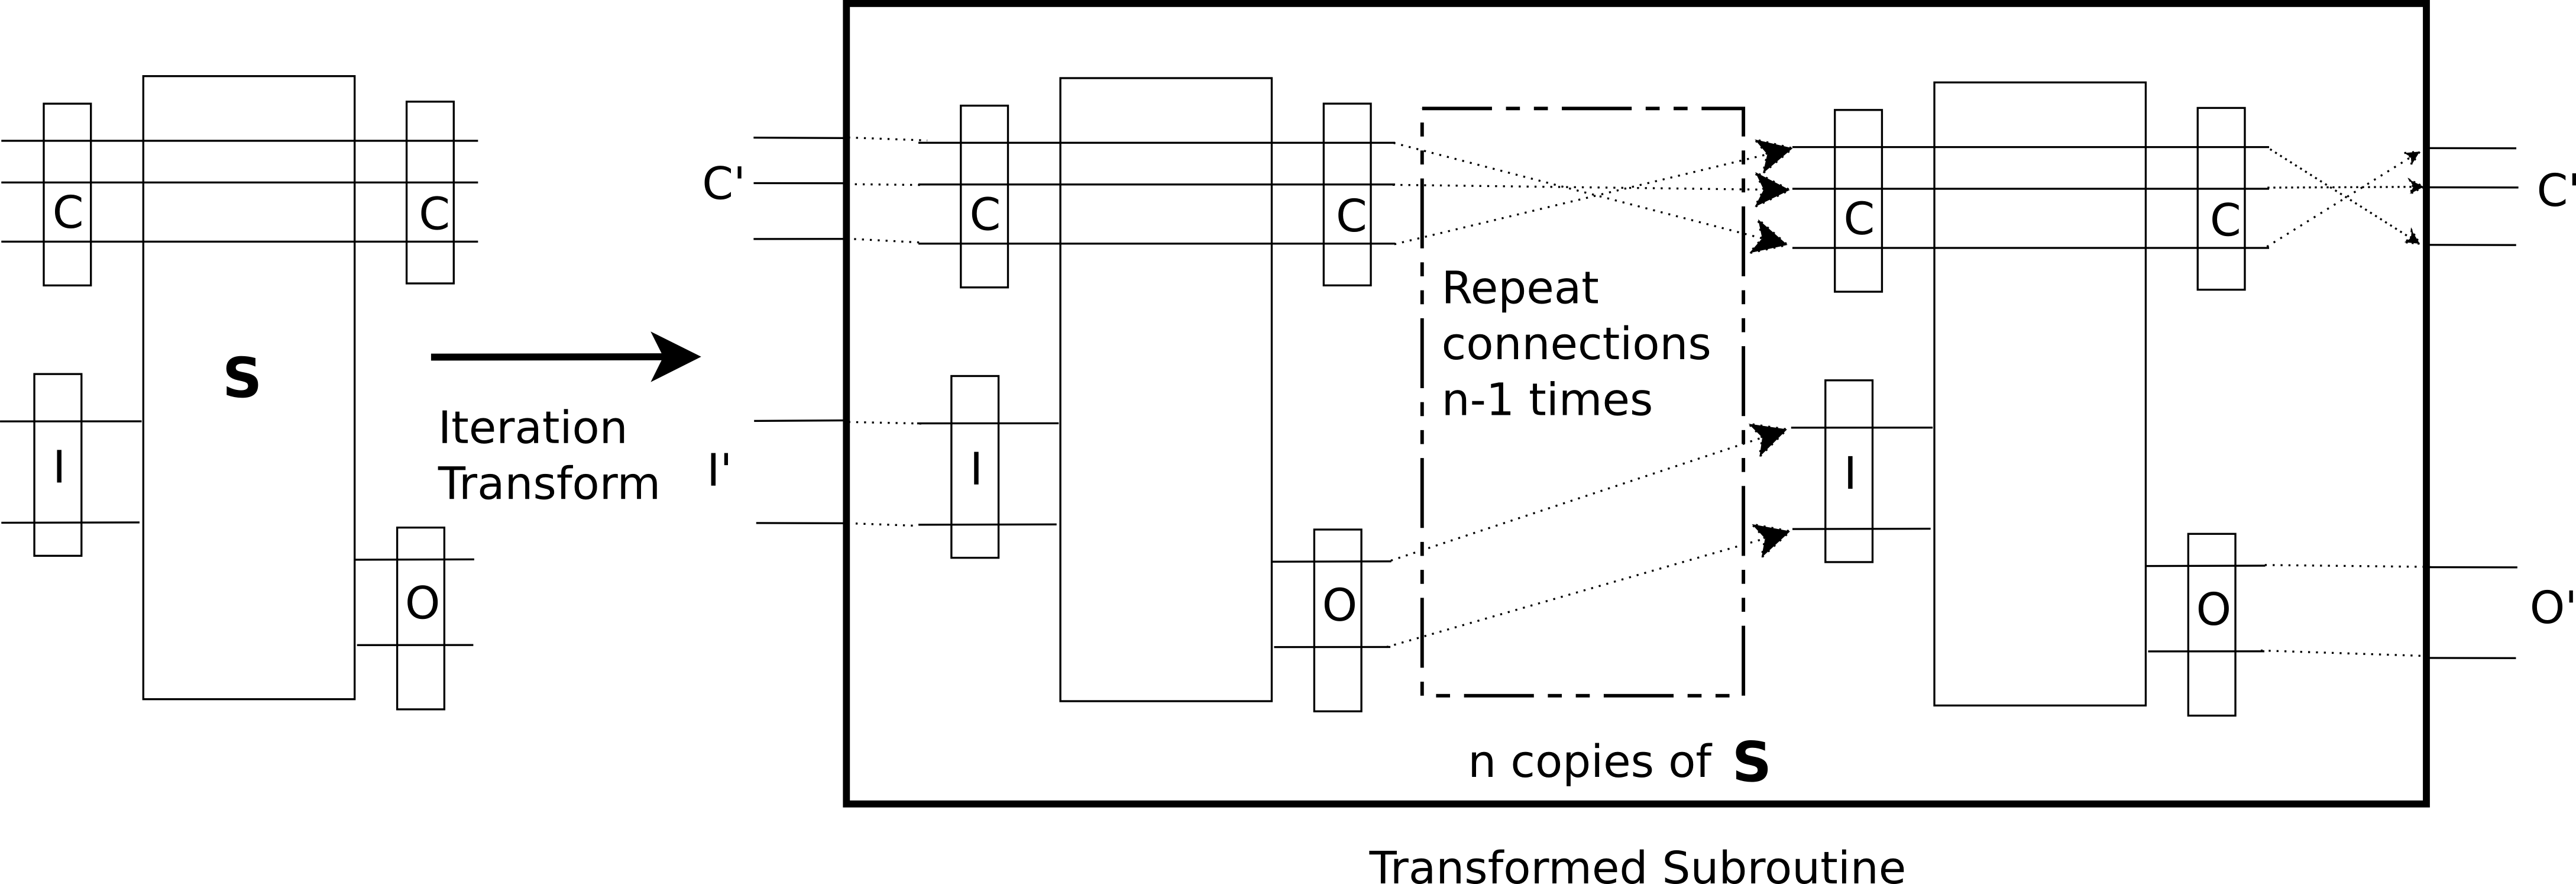
\includegraphics[scale=.4]{diagrams/SubroutineIterationTransform.png}
   \caption{Transforming a subroutine to an iterated subroutine}
   \label{fig:transforming_a_subroutine_to_an_iterated_subroutine}
\end{figure}
% subsection iteration_transformation_of_a_subroutine (end)

\subsection{Folding subroutines} % (fold)
\label{sub:folding_subroutines}

In addition to the concept of iteration the ability to fold
subroutines over data structures could also be useful. A
folded call of a subroutine is similar to an iteration, in
that controls and possibly some of the inputs
and outputs are iterated. The difference occurs in that we
expect to take some of the inputs from a data structure and
return some of the outputs to a data structure. An example of
this would be folding over a list of \qubit{s} where
each qubit is taken as a input for each iteration.

First, we will examine the requirements for a non-linear
safe fold, that is, where no input duplication on the
control wires is allow



\begin{definition}\label{def:linear_only_subroutine_fold}
  Given a subroutine $S=([gate],C,I,O,c,r,n)$, a starting context of
  typed wires $W_1$ and a data structure on wires $D\subset W_1$, a
  \emph{linear-only folded call} of $S$ over $D$ resulting in the context
  of typed wires $W_2$ and the data structure $E\subset W_2$ consists of the
  tuple $(CI_f,CO_f,  g, h, ciof_b, s_{in}, s_{out})$ where
  \begin{itemize}
    \item $CI_f::\type{Arity}, \dom{CI_f} \subset \dom{C}\cup \dom{I}$,
    \item $CO_f::\type{Arity}, \dom{CO_f} \subset \dom{C}\cup \dom{O}$,
    \item $g:\dom{C}\cup\dom I / \dom{CI_f} \to W_1$ and $g$ is injective,
    \item $h:\dom{C}\cup\dom O /\dom{CO_f} \to W_2$ and $h$ is injective
    \item $ciof_b$ is a bijection between $(\dom{C}\cup\dom{O})/\dom{CO_f}$
      and $(\dom{C}\cup\dom{I})/\dom{CI_f}$,
    \item $s_{in}: \dom{CI_f} \to W_1$ (pulls from $D$),
    \item $s_{out}: \dom{CO_f} \to W_2$ (pushes to $E$),
    \item $g + s_{in} \in F(\nothing,I,W_1)$,
    \item $ciof_b^{-1} + s_{in} \in F(\nothing,I,W_1)$,
    \item $ciof_b + s_{out} \in F(\nothing,O,W_2)$,
    \item $h + s_{out} \in F(\nothing,O,W_2)$,
    \item $|\dom{CI_f}| = leafsize(D)$,
    \item $leafsize(E) = |\dom{CO_f}|$.
  \end{itemize}
\end{definition}

\begin{definition}\label{def:structured_linear_folded_call}
  Given the data for an linear-only folded call,
  a \emph{structured linear-only folded call} is a pair of high level
  structures $(i_s,o_s)$ and $(i_{fs},o_{fs})$  and a pair of quantum
  terms $(a,b)$ such that:
  \begin{itemize}
    \item $i_s(a) = g + s_{in}$,
    \item $o_s(h + s_{out}) = b$,
    \item $i_{fs}(a) = s_{in}$, and
    \item $o_{fs}(s_{out}) = b$.
  \end{itemize}

\end{definition}

Discussion points:
\begin{itemize}
  \item Does the structured call get rid of the last two items regarding
  leafsize?  Same issue with non-linear safe call.
  \item For the structured call, it appears to me that there is only
  one pair of terms $a,b$ with two different (de)structuring morphisms.
\end{itemize}

The action on the wires of the calling program will be given by this relation:
\[
s_{out} + h \circ (s_{out} + cio_f + s_{in})^{len(D)}
\circ (g + s_{in})^{-1}.
\]
\begin{example}[Fold over Carry]\label{ex:fold_over_carry}
\end{example}

For this example, we use the carry portion of the addition algorithm found
in \cite{Vedral:1995ga}.

The carry circuit is shown below:
\[\Qcircuit @C=1em @R=.7em {
\lstick{anc} & \ctrl{2} & \qw & \qw & \rstick{anc} \qw \\
\lstick{a}  & \qw & \ctrl{1} & \ctrl{1} & \rstick{a} \qw \\
\lstick{b}  & \ctrl{1} & \targ & \ctrl{1} & \rstick{b} \qw \\
\lstick{c}  & \targ & \qw& \targ & \rstick{c} \qw
}
\]

The intent of this circuit is to compute the final carry when
adding the quregisters $A$ and $B$. The input prepares
the $anc$ in state $\ket{0}$ and an auxiliary register $R$,
the same size as $A$ and $B$ as $\ket{00\ldots0}$. Assume
that $A = [w_1,w_2,w_3], B=[w_4,w_5,w_6], anc=w_7$ and
$R=[w_8,w_9,w_{10}]$. $(A,B,R)$, a tuple of three registers
forms our $D$ --- the input to the fold. Then,
we may perform a folded call of carry as follows:
\begin{itemize}
  \item $\dom{C} = \{anc,a\},\ \dom{I} = \{b,c\} = \dom{O}$;
  \item $\dom{CI_f} = \{a,b,c\}$ and $\dom{CO_f} = \{anc,a,b\}$;
  \item $g = \{anc \mapsto w_{6}\}$, $h=\{c\mapsto w_{10}\}$
  \item $ciof_b = \{c \mapsto anc \}$
  \item $s_{in} = \{a \mapsto D[0], b \mapsto D[1], c \mapsto D[2]\}$
  \item $s_{out} = \{anc \mapsto E[2], a \mapsto E[0], b \mapsto E[1]\}$.
\end{itemize}
From the mapping $s_{out}$, we set $E = (A,B,R')$ where $R'=[w_7,w_8,w_9]$.

Discussion points:
\begin{itemize}
  \item Is there a non-linear safe use case? Carry seemed quite simple,
    but it required linear safe inputs when folded.
  \item Each fold iteration input might be multiple \qubit{s},
  combined into a single data structure, as in 
    \vref{ex:fold_over_carry}.
  \item The number of inputs and outputs no longer need
    to agree as they did in iteration.  An example would be a subroutine that
    applied a two \qubit gate and then discarded one of the \qubits.
    The fold would be expected to convert a list of pairs  of \qubit{s}
    to a list of \qubit{s}. (Note this subroutine would not be reversible
    or controllable).
  \item The shape of the foldable in and out as well as the number of \qubits
    at each leaf would need to be known.
  \item The $F(C,K,W)$ permissible functions are not quite right for
    linear-only folds --- we do not want to allow duplication of any of
    the inputs, so $F(C,K,W)$ becomes $F(\nothing,C+K,W)$.
\end{itemize}

\begin{definition}\label{def:subroutine_fold}
  Given a subroutine $S=([gate],C,I,O,c,r,n)$, a starting context of
  typed wires $W_1$ and a data structure on wires $D\subset W_1$, a
  \emph{folded call} of $S$ over $D$ resulting in the context of typed wires
  $W_2$ and the data structure $E\subset W_2$ consists of the tuple
  $(I_f,O_f, f_{in}, f_{out}, g, h, c_b, iof_b, s_{in}, s_{out} )$ where
  \begin{itemize}
    \item $I_f::\type{Arity}, \dom{I_f} \subset \dom{I}$,
    \item $O_f::\type{Arity}, \dom{O_f} \subset \dom{O}$,
    \item $f_{in}:\dom C \to W_1\cup W_2$
    \item $f_{out}:\dom C \to W_1\cup W_2$
    \item $g:\dom I / \dom{I_f} \to W_1$
    \item $h:\dom O /\dom{O_f} \to W_2$
    \item $c_b$ is a bijection (permutation) of $C$,
    \item $iof_b$ is a bijection between $\dom{O}/\dom{O_f}$
      and $\dom{I}/\dom{I_f}$,
    \item $s_{in}: \dom{I_f} \to W_1$ (pulls from $D$)
    \item $s_{out}: \dom{O_f} \to W_2$ (pushes to $E$)
    \item $f_{in}+ g+ s_{in} \in F(C,I,W_1)$,
    \item $f_{out}+ h + s_{out} \in F(C,O,W_2)$,
    \item $iof_b + s_{in} \in F(\nothing,I,W_1)$,
    \item $iof_b + s_{out} \in F(\nothing,O,W_2)$,
    \item $|\dom{I_f}| = leafsize(D)$
    \item $leafsize(E) = |\dom{O_f}|$
  \end{itemize}

\end{definition}

\begin{definition}\label{def:structured_folded_call}
  Given the data for an folded call,
  a \emph{structured folded call} is a pair of high level structures
  $(i_s,o_s)$ and $(i_{fs},o_{fs})$  and a pair of quantum
  terms $(a,b)$ such that:
  \begin{itemize}
    \item $i_s(a) = f_{in}+g + s_{in}$,
    \item $o_s(f_{out} + h + s_{out}) = b$,
    \item $i_{fs}(a) = s_{in}$, and
    \item $o_{fs}(s_{out}) = b$.
  \end{itemize}

\end{definition}

% subsection folding_subroutines (end)

\subsection{Subroutine to folded subroutine transform} % (fold)
\label{sub:subroutine_to_folded_subroutine_transform}

In order to transform a given subroutine, we require the following data:
\begin{itemize}
  \item A bijection from some subset of the control and output wires to some
  subset of the control and input wires;
  \item a count of the number of iterations.
\end{itemize}

This allows us to derive a new $C,I,O$ for the fold subroutine. We proceed
with the formal definition.
\begin{definition}\label{def:fold_transform_of_a_subroutine}
  The \emph{fold transform} of a subroutine is a function $S_f$ with
  parameters $(n,b_{cio})$ which takes the subroutine $(gates,C,I,O,r,c,n)$
  to the subroutine $(gates',C',I',O',r,c,n)$.
  The parameters have the following types:
  \begin{align*}
    n&::\type{Int}, n>0;\\
    b_{cio}&::\type{bijection(CI \leftrightarrow CO)} \\
      &\text{where }CI\subseteq C\cup I\text{ and }\subseteq C\cup O.
  \end{align*}
\end{definition}

Note that $b_{cio}$ may be defined as a set of ordered pairs
\begin{equation}
  \{(f,t)|f\in C\cup I, t \in C\cup O,\text{ and } f,t \text{ appear at most once}\}.
  \label{eq:defintion_of_bcio}
\end{equation}
The data we need to create for the end result are the set of control wires,
the input and output wires and the new gates sequence. We proceed with
presenting the algorithm for the control wires.

When considering which inputs (and hence outputs) are control wires in the
transformed subroutine, we must follow the path of a control input. A control
input to the base subroutine will remain a control input to the transformed
subroutine only if its full folded path contains only control wires before
exiting. Depending upon the structure of $b_{cio}$ it is possible all, none
or some finite subset of specific control wires become controls for the
transformed routine.

To determine if a wire is a control, we will calculate a characteristic of the
wire and show that it requires at most $k$ iterations to calculate, where
$k$ is the number of control wires of the original subroutine.

First, define:
\begin{align*}
  \Omega &:: C \to C \cup \{*,@\}\\
  \Omega(c) &=
    \begin{cases}
      c'&\text{if }b_{cio}(c) = c'\text{ and }c'\in C,\\
      *&\text{if $c$ is not the first element of any pair in }b_{cio},\\
      @&\text{if }b_{cio}(c) = j\text{ and }j\in I.
    \end{cases}
\end{align*}
Then, noting that $k = |C|$, define:
\begin{align*}
  \Gamma &:: C \to \nat \cup \{\infty\}\\
  \Gamma(c) &=
  \begin{cases}
    \infty & \Omega(c) = *,\\
    0 & \Omega(c) = @,\\
    1 + \Gamma(\Omega(c)) & \Gamma(\Omega(c)) < k,\\
    \infty & \Gamma(\Omega(c)) \ge k.
  \end{cases}
\end{align*}

Dually, we may define functions  $\Theta(c)$ and $\Delta(c)$:
\begin{align*}
\Theta &:: C \to C \cup \{*,@\}\\
\Theta(c) &=
  \begin{cases}
    c'&\text{if }b_{cio}(c') = c\text{ and }c'\in C,\\
    *&\text{if $c$ is not the second element of any pair in }b_{cio},\\
    @&\text{if }b_{cio}(o) = c\text{ and }o\in O.
  \end{cases}\\
  \Delta &:: C \to \nat \cup \{\infty\}\\
  \Delta(c) &=
  \begin{cases}
    \infty & \Theta(c) = *,\\
    0 & \Theta(c) = @,\\
    1 + \Delta(\Theta(c)) & \Delta(\Theta(c)) < k,\\
    \infty & \Delta(\Theta(c)) \ge k.
  \end{cases}
\end{align*}

Note that in the case of cycles among control wires, the cycle \emph{must} be
of size $k$ or less. As such, at most $k$ iterations of $\Gamma$ are required
before confirming a value for $\Gamma(c)$. The same argument applies to
computing $\Theta$.

Assuming that $C$ is ordered, the data for $b_{cio}$ may be stored such that
computing $b_{cio}(c)$ and therefore $\Omega(c)$ is of $\BigO{\log k}$.
Therefore, $\Gamma$ is of complexity $\BigO{k\log k}$ and computing
$\Gamma$ for all of $C$ will then be of $\BigO{k^2 \log k}$. Computing
$\Delta$ will have the same complexity.

We may now describe the  algorithm for determining control wires, $C'$
input wires, $I'$ and output wires, $O'$ of the transformed subroutine.
In the algorithm, $n$ is the number of iterations, $k$ is the cardinality
of $C$. Additionally, we compute a \emph{rank} of each $c$ in $C'$. The
\emph{rank} of $c$ is the number of iterations that $c$ will go through.
\begin{enumerate}
  \item Add all members of $I$ to $I'$, subscripting with $1$.
  \item For all $i\in I$ where $i \nin \rng b_{cio}$, add
    $i_2,i_3,\ldots,i_n$ to $I'$.
  \item Add all members of $O$ to $O'$, subscripting with $n$.
  \item For all $o\in O$ where $o \nin \dom b_{cio}$, add
    $o_1,o_2,\ldots,o_{n-1}$ to $O'$.
  \item Partition $C$ into four subsets:
  \begin{align*}
    C_*    &= \{c|c\nin \dom b_{cio}\text{ and }c\nin \rng b_{cio}\},\\
    C_d    &= \{c|c\in \dom b_{cio}\text{ and }c\nin \rng b_{cio}\},\\
    C_r    &= \{c|c\nin \dom b_{cio}\text{ and }c\in \rng b_{cio}\},\\
    C_{dr} &= \{c|c\in \dom b_{cio}\text{ and }c\in \rng b_{cio}\}.
  \end{align*}
  \item For each $c\in C_*$, add $c_1,c_2,\ldots,c_n$ to $C'$. Set the
    rank of each of these to $0$.
  \item For each $c\in C_d$, compute $j=\Gamma(c)$. If $j \ge n$, add
    $c_1,c_2,\ldots,c_n$ to $C'$. If not, then:
    \begin{itemize}
      \item Add $c_{n-j},c_{n-j+1},\ldots,c_n$ to $C'$, setting the
        rank of $c_\ell$ to $n-\ell$.
      \item Add $c_1,c_2,\ldots,c_{n-j-1}$ to $I'$.
    \end{itemize}
  \item For each $c\in C_r$, compute $m=\Delta(c)$. If $m \ge n$, add
    $c_1,c_2,\ldots,c_n$ to $C'$, setting each item to rank $0$.
    If not, then:
    \begin{itemize}
      \item Add $c_1,c_2,\ldots,c_{j+1}$ to $C'$, setting each rank to $0$.
      \item Add $c_{j+2},c_{j+3},\ldots,c_{n}$ to $I'$.
    \end{itemize}
  \item For each $c\in C_{dr}$, compute $j=\Gamma(c), m=\Delta(c)$. Then
    if $j>n-1$, add $c_1$ to $C'$, setting its rank to $n-1$, otherwise
    add it to $I'$. Conversely, if $m>n-1$, add $c_n$ to $C'$, setting its
    rank to $0$, otherwise add it to $O'$. In the case
    where both $c_1$ and $c_n$ are added to $C'$, we have actually added
    one too many items to $C'$ as there will be a duplication. This is
    addressed in the final step, where the in-out names of the control
    wires are reconciled.
  \item Reconcile the $C'$ names: For each $c_h\in C'$, compute
    $x=b_{cio}^{Rank(c)}(c)$. In $C'$, replace $x_n$ with $c_h$. After
    completing this computation, remove any duplicates.
\end{enumerate}

% The above algorithm will compute the correct $C'$ and $I'$ for the transformed
% subroutine. Additionally, we must also compute the matching of the control
% wires on input and output. To do this, we must essentially trace the path
% of each of the wires in $C'$ and determine what is the final output. There
% are three cases to consider for each $c$:
% \begin{itemize}
%   \item $\Gamma(c_m) = j>0$. This means that $c_m$ is an input with $j$ or
%     fewer iterations remaining. Compute $c' = \Omega^{rank(c_m)}(c)$. The name
%     matched with $c_m$ is then $c'_{m+rank(c_m)}$.
%   \item $\Gamma(c) = \infty, \Omega(c)=*$. $c$ is an immediate in/out control
%     wire.
%   \item $\Gamma(c) = \infty, \Omega(c)=c'$. This case occurs when $c$ is part
%     of a cycle. As noted above, the cycle must be of length $j \le k$. Hence,
%     compute $c_{\ell}=\Omega^{\ell}(c)$ where $\ell=n-1 \mod j$. Then
%     $c_\ell$ is the name of the output matched with $c$.
% \end{itemize}


% subsection subroutine_to_folded_subroutine_transform (end)
\subsection{Examples of folding} % (fold)
\label{sub:examples_of_folding}

\begin{example}\label{exmpl:fold_example_with_three_mixed_in_out}
  Consider $S=(\_,\{a,b\},\{c\},\{d\},\_,\_,\_)$ and $b_{cio}=\{(a,c),(b,a)\}$
  and an iteration count of $3$. See 
  \vref{fig:Fold_with_extra_in_out}.
\end{example}
\begin{figure}[htbp]
  \centering
    \[
\Qcircuit{
 & \dqw& \dqw &\dqw &\dqw &\dqw\ar@{.} [dddr]&\\
 & \dqw& \dqw\ar@{.}[ddr]\\
 & \multigate{3}{S_1}_{a_1} & \qw  \ar@{.}[dddr] &  & \multigate{3}{S_2}_{a_2}&\qw\ar@{.}[dddr]&  & \multigate{3}{S_3}_{a_3}&\qw\\
 & \ghost{S_1}_{b_1} & \qw \ar@{.}[ur]& &\ghost{S_2}_{b_2}&\qw\ar@{.}[ur]& &\ghost{S_3}_{b_3}&\qw\\
 &  & & & & & & & & & &\\
 & \ghost{S_1}_{c_1}& \qw_{d_1} \ar@{.}[ddr]& &\ghost{S_2}_{c_2}&\qw_{d_2}\ar@{.}[dr]& &\ghost{S_3}_{c_3}&\qw_{d_3}\\
 &            &                & &            &              & &\dqw&\dqw\\
 &            &                & & \dqw      &\dqw           &\dqw&\dqw&\dqw
}
\]
  \caption{Fold with extra in/out}
  \label{fig:Fold_with_extra_in_out}
\end{figure}

From the data, we compute:
\begin{align*}
  \Omega(a) &= @\text{ and }\Omega(b) = a,\\
  \Gamma(a) &=0\text{ and }\Gamma(b) = 1,\\
  \Theta(b) &=*\text{ and }\Delta(b)=\infty,\\
  \Theta(a)=b\text{ and } \Delta(a)=\infty.
\end{align*}

Now, following the steps of the algorithm,
\begin{enumerate}
  \item $I' \mapsto \{c_1\}$.
  \item No change to $I'$.
  \item $O' \mapsto \{d_3\}$.
  \item $O' \mapsto \{d_1,d_2,d_3\}$.
  \item $C_*=\nothing, C_d=\{b\}, C_r =\nothing, C_{dr}=\{a\}$.
  \item For $C_d$, As $\Gamma(b)=1$, we have $C' \mapsto \{b_2,b_3\}$ and
    $I' \mapsto \{c_1,b_1\}$. The rank of $b_2$ is 1 and the rank of $b_3$
    is 0.
  \item For $C_{dr}=\{a\}$, $\Gamma(a)=0$ and $\Delta(a)=\infty$, therefore
    we add $a_1$ to $I'$ and $a_3$ to $C'$. The rank of $a_3$ is zero.
    At this stage, we now have
    $I'=\{c_1,b_1,a_1\}, O'=\{d_1,d_2,d_3\}$ and $C'=\{b_2,b_3,a_3\}$.
  \item Reconcile $C'$: $b_{cio}(b)=a$ and $b_{cio}(a)=c$, therefore
    $b_{cio}^1(b_2)=a_3$, $b_{cio}^0(b_3)=b_3$, and $b_{cio}^0(a_3)=a_3$.
    Following our replacement scheme, $C'=\{b_2,b_3\}$.
\end{enumerate}

Hence our final result is:
\begin{align*}
  I'&=\{c_1,b_1,a_1\},\\
  O'&=\{d_1,d_2,d_3\}\text{ and}\\
  C'&=\{b_2,b_3\}.
\end{align*}

\begin{example}\label{exmpl:fold_example_with_partial_bcio}
  Consider $S=(\_,\{a,b\},\{c\},\{d\},\_,\_,\_)$ as in 
  \vref{exmpl:fold_example_with_three_mixed_in_out} and
  $b_{cio}=\{(a,c),(b,a),(d,b)\}$ and an iteration count of $3$. See 
  \vref{fig:Fold_with_three_iterations}.
\end{example}
\begin{figure}[htbp]
  \centering
    \[
\Qcircuit{
 & \multigate{3}{S_1}_{a_1} & \qw  \ar@{.}[dddr] &  & \multigate{3}{S_2}_{a_2}&\qw\ar@{.}[dddr]&  & \multigate{3}{S_3}_{a_3}&\qw\\
 & \ghost{S_1}_{b_1} & \qw \ar@{.}[ur]& &\ghost{S_2}_{b_2}&\qw\ar@{.}[ur]& &\ghost{S_3}_{b_3}&\qw\\
 &  & & & & & & & & & &\\
 & \ghost{S_1}_{c_1}& \qw_{d_1} \ar@{.}[uur]& &\ghost{S_2}_{c_2}&\qw_{d_2}\ar@{.}[uur]& &\ghost{S_3}_{c_3}&\qw_{d_3}\\
}
\]
\caption{Fold with three iterations}
  \label{fig:Fold_with_three_iterations}
\end{figure}

From the data, we have:
\begin{align*}
  \Omega(a) &= @\text{ and }&\Gamma(a)=0,\\
  \Omega(b) &= a\text{ and }&\Gamma(b) = 1,\\
  \Theta(b)&=@\text{ and }&\Delta(b)=0,\\
  \Theta(a)&=b\text{ and }&\Delta(a)=1.
\end{align*}

Now, following the steps of the algorithm,
\begin{enumerate}
  \item $I' \mapsto \{c_1\}$.
  \item No change to $I'$.
  \item $O' \mapsto \{d_3\}$.
  \item All $o$ are in the range of $b_{cio}$, therefore no further
    change to $O'$.
  \item $C_*=C_d=C_r = \nothing, C_{dr}=\{a,b\}$.
  \item As $n-1=2 > \Gamma(a),\Gamma(b)$, we have $I'
    \mapsto \{c_1,a_1,b_1\}$. Similarly, since $n-1=2 > \Delta(a),\Delta(b)$,
    $O'\mapsto \{a_3,b_3,d_3\}$
  \item With $C'$ empty, there are no further steps.
\end{enumerate}
Hence our final result is:
\begin{align*}
  I'&=\{c_1,b_1,a_1\},\\
  O'&=\{a_3,b_3,d_3\}\text{ and}\\
  C'&=\nothing.
\end{align*}

\begin{example}\label{exmpl:fold_transform_example_of_carry}
  Consider $C=(\_,\{r,a\},\{b,c\},\{d,e\},\_,\_,\_)$,
  $b_{cio}=\{(e,r)\}$ and an iteration count of $4$. See 
  \vref{fig:fold_carry_transformed}.
\end{example}
\begin{figure}[htbp]
  \centering
    \[
\xymatrix @R=7pt @*=<0em>{
 & \multigate{3}{C}_{r_1} & \qw& \qw & \qw & \qw & \qw & \qw & \qw\\
 & \ghost{C}_{a_1} & \qw       & \qw & \qw & \qw & \qw & \qw & \qw\\
 & \ghost{C}_{b_1} & \qw_{d_1} & \qw & \qw & \qw & \qw & \qw & \qw\\
 & \ghost{C}_{c_1} & \qw_{e_1} & \multigate{3}{C}_{r_2} & \qw & \qw & \qw & \qw  & \qw\\
 & \qw_{a_2}       & \qw       & \ghost{C} & \qw        & \qw & \qw & \qw & \qw\\
 & \qw_{b_2}       & \qw       & \ghost{C} & \qw_{d_2}  & \qw & \qw & \qw & \qw \\
 & \qw_{c_2}       & \qw       & \ghost{C} & \qw_{e_2}  & \multigate{3}{C}_{r_3} &\qw& \qw & \qw\\
 & \qw_{a_3}       & \qw       & \qw       & \qw        & \ghost{C} &\qw      & \qw & \qw \\
 & \qw_{b_3}       & \qw       & \qw       & \qw        & \ghost{C} &\qw_{d_3}& \qw & \qw\\
 & \qw_{c_3}       & \qw       & \qw       & \qw        & \ghost{C} &\qw_{e_3}& \multigate{3}{C}_{r_4} &\qw\\
 & \qw_{a_4}       & \qw       & \qw       & \qw        & \qw       & \qw     & \ghost{C} &\qw\\
 & \qw_{b_4}       & \qw       & \qw       & \qw        & \qw       & \qw     & \ghost{C} &\qw_{d_4}\\
 & \qw_{c_4}       & \qw       & \qw       & \qw        & \qw       & \qw     & \ghost{C} &\qw_{e_4}\\
}
\]
  \caption{Fold of Carry}
  \label{fig:fold_carry_transformed}
\end{figure}

From the data, we have:
\begin{align*}
  \Omega(r) &= *\text{ and }&\Omega(a) = *,\\
  \Gamma(r)&=\infty\text{ and }&\Gamma(a) = \infty,\\
  \Theta(r)&=@\text{ and }&\Delta(r)=0,\\
  \Theta(a)=*\text{ and } &\Delta(a)=\infty.
\end{align*}

Now, following the steps of the algorithm,
\begin{enumerate}
  \item $I' \mapsto \{b_1,c_1\}$.
  \item No element of $I$ appears in $b_{cio}$, therefore we now have
    $I' \mapsto \{b_1,c_1,b_2,c_2,b_3,c_3,b_4,c_4\}$
  \item $O' \mapsto \{d_4,e_4\}$.
  \item Only $e$ is in the range of $b_{cio}$, therefore we add
  $d_1,d_2,d_3$ to  $O'$, giving us $\{d_1,d_2,d_3,d_4,e_4\}$.
  \item $C_*=\{a\},C_d=\nothing, C_r = \{r\},\ C_{dr}=\nothing$.
  \item Considering $C_*$, we add $\{a_1,a_2,a_3,a_4\}$ to $C'$, each with
    rank 0.
  \item Next considering $C_r$, as $\Delta(r)=0$, we add $r_1$ to $C'$ with
    rank 0 and then add $r_2,r_3,r_4$ to $O'$.
  \item As each element of $C'$ is of rank 0, there is no changes
    to the names.
\end{enumerate}

Hence our final result is:
\begin{align*}
  I'&=\{b_1,c_1,b_2,c_2,b_3,c_3,b_4,c_4\},\\
  O'&=\{d_1,d_2,d_3,d_4,e_4,r_2,r_3,r_4\}\text{ and}\\
  C'&=\{r_1,a_1,a_2,a_3,a_4\}.
\end{align*}

% subsection examples_of_folding (end)
% section subroutine_calls_and_transformers (end)

% section diagram_of_folded_carry (end)
\section{Alternate Algorithm for Fold Transformation} % (fold)
\label{sec:alternate_algorithm_for_fold_transformation}
In  this section, we present an alternate algorithm for calculating the
type and names of control, input and output wires for a folded
subroutine.  The starting point is 
\vref{def:fold_transform_of_a_subroutine}
and the ordered pairs of $b_{cio}$: A set of ordered pairs
$\{(f,t)|f\in C\cup I, t \in C\cup O\}$.

To implement the algorithm of calculating the folded subroutines $C,I$ and
$O$, we need the following:
\begin{itemize}
  \item $I\cap O = \nothing$, which may be accomplished by renaming if needed.
  \item We create the sets $C_j,I_j,O_j$ for $j=1\ldots n$ where the members
    of $X_j$ are the elements of $X$ together with the subscript $j$ where
    $X$ is one of $C,I,O$.
\end{itemize}

The algorithm proceeds by creating a set of ``type'' constraints for each of
the elements of the new sets, based upon $b_{cio}$ and membership in a $C,I$
or $O$ set.

The algorithm steps are:
\begin{enumerate}
  \item Create a set $\mathcal{C}$ of pairs $(a_j,b_{j+1})$ for $j$
  ranging from $0$ to $n-1$ based upon the bijection $b_{cio}$.
  \item For each $j=0\ldots n-1$,
  \begin{enumerate}
    \item For all $c\in C_j$, if $(c,\_)\notin\mathcal{C}$,
      add the pair $(c,\nothing)$
    \item For all $c\in C_j$, if $(\_,c)\notin\mathcal{C}$,
      add the pair $(\nothing,c)$
    \item For all $o\in O_j$, if $(o,\_)\notin\mathcal{C}$,
      add the pair $(o,\nothing)$
    \item For all $i\in I_j$, if $(\_,i)\notin\mathcal{C}$,
      add the pair $(\nothing,i)$
  \end{enumerate}
  \item Convert the pairs in $\mathcal{C}$ to equations and constraints as
    follows for each pair $(a,b)$:
  \begin{enumerate}
    \item $a=\nothing\implies \begin{cases}
      b::(b,C)&\text{when }b\in C_j\text{for some }j,\\
      b::(b,I)&\text{when }b\in I_j\text{for some }j.
    \end{cases}$
    \item $a\in C_{j-1}\implies \begin{cases}
      b=a&\text{when }b\in C_j,\\
      b=a, b::I&\text{when }b\in I_j,\\
      a::(C,a)&\text{when }b=\nothing.
    \end{cases}$
    \item $a\in O_{j-1}\implies \begin{cases}
      b=a, b::O&\text{when }b\in C_j,\\
      \text{no equation}&\text{when }b\in I_j,\\
      a::(O,a)&\text{when }b=\nothing.
    \end{cases}$
  \end{enumerate}
  \item Solve the equations with the constraints, with the assumption that
    \[\xymatrix{
      &C\ar[dl]\ar[dr] \ar[d] & \\
      I \ar[dd]&(C,b)\ar[dr] \ar[d]&O\ar[d] \\
      &(b,C)\ar[dl]& (O,b) \\
      (b,I)& & }
    \]
  For example,
  \begin{itemize}
    \item $a::O, a::C$ is solvable with $a::O$;
    \item $a=b,b::(b,C),a::I$ is solved by $b,a::(b,I)$;
    \item $a=b, b=d, a::(a,C), d::(C,d)$ is solved by $a,b,d::(a,C)$.
  \end{itemize}
  \item For the folded subroutine, $X$ will be all items of ``type'' $X$,
    where $X$ is any of $C,I,O$, the names of each entry will be the companion
    name with the ``type''.
\end{enumerate}
\note{The algorithm above works correctly, but likely has too high of a
complexity, depending on the number of iterations. Need to revise in the
next version to see if we can make the complexity proportional to the number
of wires in/out.}
\subsection{Examples of folding with Alternate Algorithm} % (fold)
\label{sub:examples_of_folding_with_alternate_algorithm}
\begin{example}\label{exmpl:alternate_fold_example_with_three_mixed_in_out}
  We repeat \vref{exmpl:fold_example_with_three_mixed_in_out}, that is,
  $S=(\_,\{a,b\},\{c\},\{d\},\_,\_,\_)$ and $b_{cio}=\{(a,c),(b,a),(d,b)\}$
  and an iteration count of $3$. See 
  \vref{fig:Fold_with_three_iterations}.
\end{example}
There are two control wires $a,b$, an input wire $d$ and one output
wire $d$. We  will do three iterations. Our set $\mathcal{C}$ of pairs
becomes:
\begin{align*}
  \{ & (\nothing,a),\ (\nothing,b),\ (\nothing,c),\\
  & (b,a_1),\ (d,b_1),\ (a,c_1),\\
  & (b_1,a_2),\ (d_1,b_2),\ (a_1,c_2),\\
  & (a_2,\nothing),\ (b_2,\nothing),\ (c_2,\nothing)\}.\\
\end{align*}
Translating each of these to equations and constraints, we get:
\begin{align*}
  &a::(a,C), b::(b,C), c::(c,I)\\
  &b=a_1, b_1=d\ b_1::O, a=c_1\ c_1::I\\
  &b_1=a_2, b_2=d_1\ b_2::O, a_1=c_2\ c_2::I\\
  &a_2::(C,a_2), b_2::(C,b_2), d_2::(O,d_2)
\end{align*}
As we have three wires in and three wires out, we expect to see six separate
groupings in the solution to the above equations. We will proceed by starting
from the top left.
\begin{align*}
  \text{start: }a &\quad a=c_1, ::I, ::(a,C) &\implies a::(a,I)\\
  \text{start: }b &\quad  b=a_1,a_1=c_2, ::I, ::(b,C) &\implies b::(b,I)\\
  \text{start: }c &\quad  ::(c,I) &\implies c::(c,I)\\
  \text{start: }b_1 &\quad  b_1=d, b_1=a_2, ::O, ::(C,a_2) &\implies
    a_2::(O,a_2)\\
  \text{start: }b_2 &\quad  b_2=d_1, ::O, ::(C,b_2) &\implies b_2::(O,b_2)\\
  \text{start: }d_2 &\quad  ::(O,d_2) &\implies d_2::(O,d_2)
\end{align*}
% subsection examples_of_folding (end)
% section alternate_algorithm_for_fold_transformation (end)


%!TEX root = /Users/gilesb/UofC/thesis/phd-thesis/phd-thesis.tex
\chapter{Synthesis of quantum operations} % (fold)
\label{cha:synthesis_of_quantum_operations}

\section{Introduction to synthesis} % (fold)
\label{sec:introduction_to_synthesis}
An important problem in quantum information theory is the decomposition of arbitrary unitary
operators into gates from some fixed universal set {\cite{neilsen2000:QuantumComputationAndInfo}}.
Depending on the operator to be decomposed, this may either be done exactly or to within some given
accuracy $\epsilon$; the former problem is known as {\em exact synthesis} and the latter as {\em
approximate synthesis} {\cite{Kliuchnikov-et-al}}.

% section introduction_to_synthesis (end)

\section{Exact synthesis of single qubit operators} % (fold)
\label{sec:exact_synthesis_of_single_qubit_operators}


Matsumoto and Amano {\cite{MA08}} showed that every single-qubit Clifford+$T$ operator can be
uniquely written in the following form, which we call the {\em Matsumoto-Amano normal form:}
\begin{equation}\label{eqn-ma}
 (T\mid\emptyseq)\,(HT\mid SHT)^*\,{\cC}.
\end{equation}
Here, we have used the syntax of regular expressions {\cite{regexp}} to denote a set of sequences
of operators. The symbol $\varepsilon$ denotes the empty sequence (more precisely, the singleton
set containing just the empty sequence); if $\cL$ and $\cK$ are two sets of sequences, then
$\cL\mid \cK$ denotes their union; $\cL \cK$ denotes the set $\s{st\mid s\in\cL, t\in\cK}$; $\cL^*$
denotes the set $\s{s_1\ldots s_n \mid n\geq 0; s_1,\ldots,s_n\in\cL}$; and $\cC$ denotes any
Clifford operator. In words, the Matsumoto-Amano representation of an operator consists of a
Clifford operator, followed by any number of {\em syllables} of the form $HT$ or $SHT$, followed by
an optional syllable $T$. (We follow the usual convention of multiplying operators right-to-left,
so when we say one operator ``follows'' another, we mean that it appears to its left).

The most important properties of the Matsumoto-Amano decomposition are:
\begin{itemize}
  \item Existence: every single-qubit Clifford+$T$ operator can be written in Matsumoto-Amano
    normal form (moreover, there is an efficient algorithm for converting the operator to normal
    form);

  \item Uniqueness: no operator can be written in Matsumoto-Amano normal form in more than one way;

  \item $T$-optimality: of all the possible exact decompositions of a given operator into the
    Clifford+$T$ set of gates, the Matsumoto-Amano normal form contains the smallest possible number
    of $T$-gates.
\end{itemize}
It is perhaps less well-known that the uniqueness proof given by Matsumoto and Amano yields an
efficient {\em algorithm} for $T$-optimal exact single-qubit synthesis. One may contrast this, for
example, with the recent algorithm by Kliuchnikov et al.~{\cite{Kliuchnikov-et-al}}, which is
efficient, but only asymptotically $T$-optimal. The purpose of this note is to give a detailed
presentation of the algorithmic content of Matsumoto and Amano's result. Along the way, we also
simplify Matsumoto and Amano's proofs, and we give an intrinsic characterization of the
Clifford+$T$ subgroup of $SO(3)$.

\subsection{Existence} % (fold)
\label{sub:existence}
In the following, we will often speak of sequences of operators. For our purposes, a sequence is
just an $n$-tuple. We write $st$ for the operation of concatenating two sequences, and we write
$\emptyseq$ for the empty sequence. We identify a 1-tuple $(A)$ with the operator $A$ itself. If
$s=\tuple{A_1,\ldots,A_n}$ is a sequence of operators, we write $\sem{s}=A_1\cdots A_n$ for the
product of the operators in the sequence; naturally, $\sem{\emptyseq}=I$. Note that the notation is
ambiguous; for example, depending on the context, $SHT$ may denote either the sequence
$\tuple{S,H,T}$ of 3 operators, or their product, which is a single operator. To alleviate the
ambiguity, we assume that everything is a sequence by default, and we write $s\seqeq t$ if two
sequences are equal as tuples, and $s=t$ if they are equal as operators, i.e., if $\sem{s}=\sem{t}$.

\begin{remark}
  Consider any operator $A$ in Matsumoto-Amano normal form. If $\lambda$ is any unit scalar, then
  $\lambda A$ can clearly also be written in Matsumoto-Amano normal form with the same $T$-count,
  namely by multiplying $\lambda$ into the rightmost Clifford operator. Moreover, if $A$ can be
  {\em uniquely} written in Matsumoto-Amano normal form, then the same is true for $\lambda A$.
  Therefore, nothing is added or lost to the Matsumoto-Amano normal form whether one allows
  arbitrary global phases, a suitable discrete set of global phases (for example, powers of
  $e^{i\pi/4}$), or whether one works modulo global phase. Since it is convenient to work modulo
  global phase, we do so in the remainder; however, this does not restrict the generality of the
  results.
\end{remark}

\begin{definition}
  Let $\sC$ denote the Clifford group on one qubit, modulo global phases. This group has 24
  elements. Let $\sS$ be the 8-element subgroup spanned by $S$ and $X$. Let $\sCp = \sC\sm\sS$. Let
  $\sH = \s{I,H,SH}$ and $\sHp = \s{H,SH}$.
\end{definition}

\begin{lemma}\label{lem-SH}
  The following hold:
  \begin{align}
    \sC ~&=~ \sH\sS,\label{eqn-CHS}\\
    \sCp ~&=~ \sHp\sS,\label{eqn-CSHS}\\
    \sS\sHp ~&\seq~ \sHp\sS,\label{eqn-SHHS}\\
    \sS T ~&=~ T \sS,\label{eqn-STTS}\\
    T \sS T ~&=~ \sS.\label{eqn-TSTS}
  \end{align}
\end{lemma}

\begin{proof}
  Since $\sS$ is an 8-element subgroup of $\sC$, it has three left cosets. They are $\sS$, $H\sS$,
  and $SH\sS$. Since $\sC$ is the disjoint union of these cosets, (\ref{eqn-CHS}) and
  (\ref{eqn-CSHS}) immediately follow. For (\ref{eqn-SHHS}), first notice that $\sS S=\sS$, and
  therefore $\sS\sHp = \sS H\cup \sS SH = \sS H$. Since $\sS H$ is a non-trivial right coset of
  $\sS$, it follows that $\sS H \seq \sC\sm\sS = \sCp$. Combining these facts with
  (\ref{eqn-CSHS}), we have (\ref{eqn-SHHS}). Finally, the equations (\ref{eqn-STTS}) and
  (\ref{eqn-TSTS}) are trivial consequences of the equations $ST=TS$, $XT=TXS$, and $TT=S$.
\end{proof}

\begin{proposition}[Matsumoto and Amano {\cite{MA08}}]\label{prop-ma}
  Every single-qubit Clifford+$T$ operator can be written in Matsumoto-Amano normal form.
\end{proposition}

\begin{proof}
  Let $M$ be a single-qubit Clifford+$T$ operator. Clearly, $M$ can be written as
  \begin{equation}\label{eqn-M}
    M = C_n\;T\;C_{n-1}\;\cdots\;C_1\;T\;C_0,
  \end{equation}
  for some $n\geq 0$, where $C_0,\ldots,C_n\in\sC$. First note that if $C_i\in\sS$ for any
  $i\in\s{1,\ldots,n-1}$, then we can immediately use (\ref{eqn-TSTS}) to replace $TC_iT$ by a
  single Clifford operator. This yields a shorter expression of the form (\ref{eqn-M}) for $M$. We
  may therefore assume without loss of generality that $C_i\not\in\sS$ for $i=1,\ldots,n-1$. If
  $n=0$, then $M$ is a Clifford operator, and there is nothing to show. Otherwise, we have
  \begin{align}
    M ~&\in~ \sC\;T\;\sCp\;\cdots\;\sCp\;T\;\sC &&\mbox{ by (\ref{eqn-M})}\\
    &=~ \sH\sS\;T\;\sHp\sS\;\cdots\;\sHp\sS\;T\;\sC &&\mbox{ by
      (\ref{eqn-CHS}) and (\ref{eqn-CSHS})}\\
    &\seq~ \sH\;T\;\sHp\;\cdots\;\sHp\;T\;\sC &&\mbox{ by
      (\ref{eqn-SHHS}) and (\ref{eqn-STTS}).}\label{eqn-HTHpTC}
  \end{align}
  Note how, in the last step, the relations (\ref{eqn-SHHS}) and (\ref{eqn-STTS}) were used to move
  all occurrences of $\sS$ to the right, where they were absorbed into the final $\sC$. It is now
  trivial to see that every element of (\ref{eqn-HTHpTC}) can be written in Matsumoto-Amano normal
  form, finishing the proof.
\end{proof}

\begin{corollary}\label{cor-efficient}
  There exists a linear-time algorithm for symbolically reducing any sequence of Clifford+$T$
  operators to Matsumoto-Amano normal form. More precisely, this algorithm runs in time at most
  $O(n)$, where $n$ is the length of the input sequence.
\end{corollary}

\begin{proof}
  The proof of Proposition~\ref{prop-ma} already contains an algorithm for reducing any sequence of
  Clifford+$T$ operators to Matsumoto-Amano normal form. However, in the stated form, it is perhaps
  not obvious that the algorithm runs in linear time. Indeed, a naive implementation of the first
  step would require up to $n$ searches of the entire sequence for a term of the form $T\sS T$,
  which can take time $O(n^2)$.

  One obtains a linear time algorithm from the following observation: if $M$ is already in
  Matsumoto-Amano normal form, and $A$ is either a Clifford operator or $T$, then $MA$ can be
  reduced to Matsumoto-Amano normal form in constant time. This is trivial when $A$ is a Clifford
  operator, because it will simply be absorbed into the rightmost Clifford operator of $M$. In the
  case where $A=T$, a simple case distinction shows that at most the rightmost 5 elements of $MA$
  need to be updated. The normal form of a sequence of operators $A_1A_2\ldots A_n$ can now be
  computed by starting with $M=I$ and repeatedly right-multiplying by $A_1,\ldots,A_n$, reducing to
  normal form after each step.
\end{proof}

% subsection existence (end)

\subsection{$T$-Optimality} % (fold)
\label{sub:_t_optimality}
\begin{corollary}
  Let $M$ be an operator in the Clifford+$T$ group, and assume that $M$ can be written with
  $T$-count $n$. Then there exists a Matsumoto-Amano normal form for $M$ with $T$-count at most $n$.
\end{corollary}

\begin{proof}
  This is an immediately consequence of the proof of Proposition~\ref{prop-ma}, because the
  reduction from (\ref{eqn-M}) to (\ref{eqn-HTHpTC}) does not increase the $T$-count.
\end{proof}

% subsection _t_optimality (end)

\subsection{Uniqueness} % (fold)
\label{sub:uniqueness}
\begin{theorem}[Matsumoto and Amano {\cite{MA08}}]\label{thm-ma}
  If $M$ and $N$ are two different Matsumoto-Amano normal forms, then they describe different
  operators.
\end{theorem}

Recall that each single-qubit unitary operator (modulo global phase) can be uniquely represented as
a rotation on the Bloch sphere, or equivalently, as an element of $SO(3)$, the real orthogonal
$3\times 3$ matrices with determinant 1. The relationship between an operator $U\in U(2)$ and its
Bloch sphere representation $\hat U\in SO(3)$ is given by
\begin{equation}\label{eqn-bloch-conversion}
  \hat U\zmatrix{c}{x\\y\\z} ~=~ \zmatrix{c}{x'\\y'\\z'}
  \quad\Longleftrightarrow\quad
  U\,(xX+yY+zZ)\;U\da ~=~ x'X + y'Y + z'Z,
\end{equation}
where $X$, $Y$, and $Z$ are the Pauli operators. The Bloch sphere representations of the operators
$H$, $S$, and $T$ are:
\begin{equation}\label{bloch-generators}
  \hat H = \zmatrix{ccc}{0&0&1\\0&-1&0\\1&0&0}, \quad
  \hat S = \zmatrix{ccc}{0&-1&0\\1&0&0\\0&0&1}, \quad
  \hat T = \frac{1}{\sqrt{2}}\zmatrix{ccc}{1&-1&0\\1&1&0\\0&0&\sqrt{2}}.
\end{equation}
\begin{remark}\label{rem-bloch}
  The Bloch sphere representation of any scalar is the identity matrix. The Bloch sphere
  representations of the 24 Clifford operators (modulo phase) are precisely those elements of
  $SO(3)$ that can be written with matrix entries in $\s{-1,0,1}$; these are exactly the 24
  symmetries of the cube $\s{(x,y,z)\mid -1\leq x,y,z\leq 1}$.
\end{remark}

\begin{definition}
  Recall that $\N$ denotes the natural numbers including 0; $\Z$ denotes the integers; and $\Z_2$
  denotes the integers modulo 2. We define three subrings of the real numbers:
  \begin{itemize}
    \item $\D = \Z[\frac12] = \s{\frac{a}{2^n}\mid a\in\Z,
        n\in\N}$. This is the ring of {\em dyadic fractions}.
    \item $\Zs = \s{a+b\sqrt 2 \mid a,b\in\Z}$. This is the ring of {\em
        quadratic integers} with radicand 2.
    \item $\Ds = \Z[\frac1{\sqrt2}] = \s{r+s\sqrt 2 \mid r,s\in\D}$.
  \end{itemize}
  We will also need a fourth ring, which is not a subring of the real numbers.
  \begin{itemize}
    \item $\Zss = \s{a+b\sqrt 2 \mid a,b\in\Z_2}$.
  \end{itemize}
  Note that the ring $\Zss$ has only 4 elements; they are residue classes modulo 2 of the ring
  $\Z[\sqrt 2]$. For brevity, we refer to the elements of $\Zss$ as {\em residues}.
\end{definition}


\begin{definition}[Residue\footnote{I don't think we need residue here,
  which is good as it will then be used only in section 7, the $U(2)$ case}
  and parity]
  Consider the unique ring homomorphism $\Z\to\Z_2$, mapping $a\in\Z$ to $\bar a\in\Z_2$, where
  $\bar a=0$ if $a$ is even and $\bar a=1$ if $a$ is odd. This induces a surjective ring
  homomorphism $\rho:\Zs\to\Zss$, defined by $\rho(a+b\sqrt{2}) = \bar a + \bar b\sqrt{2}$. For any
  given $x\in\Zs$, we refer to $\rho(x)$ as the {\em residue of $x$}.

  Moreover, consider the ring homomorphism $p:\Zs\to\Z_2$ given by $p(a+b\sqrt{2}) = \bar a$. We
  refer to $p(x)$ as the {\em parity} of $x$.
\end{definition}

\begin{definition}[Denominator exponent]
  For every element $q\in\Ds$, there exists some natural number $k\geq 0$ such that
  $\sqrt{2}^kq\in\Zs$, or equivalently, such that $q$ can be written as $\frac{x}{\sqrt{2}^k}$, for
  some quadratic integer $x$. Such $k$ is called a {\em denominator exponent} for $q$. The least
  such $k$ is called the {\em least denominator exponent} of $q$.

  More generally, we say that $k$ is a denominator exponent for a vector or matrix if it is a
  denominator exponent for all of its entries. The least denominator exponent for a vector or
  matrix is therefore the least $k$ that is a denominator exponent for all of its entries.
\end{definition}

\begin{definition}[$k$-parity]
  Let $k$ be a denominator exponent for $q\in\Ds$. We define the {\em $k$-residue} of $q$, in
  symbols $\rho_k(q)\in \Zss$, and the {\em $k$-parity} of $q$, in symbols $p_k(q)\in\Z_2$, by
  \[
    \rho_k(q) = \rho(\sqrt{2}^k q),
    \hspace{0.5in}
    p_k(q) = p(\sqrt{2}^k q).
  \]
  The $k$-residue and $k$-parity of a vector or matrix are defined componentwise.
\end{definition}

% ......................................................................
\begin{figure}
  \[
  \xymatrix{
    *+{\makebox[0in][r]{Start:~}\zmatrix{ccc}{1&0&0 \\ 0&1&0 \\ 0&0&1}}
    \ar[d]^<>(.5){\displaystyle T}_<>(.5){k\pp}
    \ar@<1.5ex>@(dr,r)[]+R_<>(.53){\displaystyle \sC}
    \\
    *+{\zmatrix{ccc}{1&1&0 \\ 1&1&0 \\ 0&0&0}}
    \ar@<-0.5ex>@/_/[d]_<>(.5){\displaystyle H}
    \\
    *+{\zmatrix{ccc}{0&0&0 \\ 1&1&0 \\ 1&1&0}}
    \ar[r]_<>(.5){\displaystyle S}
    \ar@<-0.5ex>@/_/[u]_<>(.6){\displaystyle T}_<>(.25){k\pp}
    &
    *+{\zmatrix{ccc}{1&1&0 \\ 0&0&0 \\ 1&1&0}}
    \ar@<-2ex>@/_4ex/[ul]_<>(.5){\displaystyle T}^<>(.5){k\pp}
  }
  \]
  \caption{The action of Matsumoto-Amano normal forms on
    $k$-parities. All matrices are written modulo the right action
    of the Clifford group, i.e., modulo a permutation of the
    columns.}\label{fig-so3-action}
\end{figure}
% ......................................................................

\begin{remark}
  Let $C$ be any Clifford operator, and $\hat C$ its Bloch sphere representation. As noted above,
  the matrix entries of $\hat C$ are in $\s{-1,0,1}$; it follows that $\hat C$ has denominator
  exponent 0. In particular, it follows that multiplication by $\hat C$ is a well-defined operation
  on parity matrices: for any $3\times 3$-matrix $U$ with entries in $\Zss$, we define $U\bullet C
  := U\cdot p(\hat C)$. This defines a right action of the Clifford group on the set of parity
  matrices.
\end{remark}

\begin{definition}\label{def-simg}
  If $G$ is any subgroup of the Clifford group, we define $\sim_G$ the be the equivalence relation
  induced by this right action, i.e., for parity matrices $U,V$, we write $U\sim_G V$ if there
  exists some $C\in G$ such that $V=U\bullet G$. In case $G=\sC$ is the entire Clifford group,
  $U\sim_{\sC} V$ holds if and only if $U$ and $V$ differ by a permutation of columns.
\end{definition}

\begin{lemma}\label{lem-ma}
  Let $M$ be a Matsumoto-Amano normal form, and $\hat M\in SO(3)$ the Bloch sphere operator of $M$.
  Let $k$ be the least denominator exponent of $\hat M$. Then exactly one of the following holds:\rm
  \begin{itemize}
    \item $k=0$, and $M$ is a Clifford operator.
    \item $k>0$, $p_k(\hat M)\sim_{\sC} \zmatrix{ccc}{1&1&0 \\ 1&1&0 \\
        0&0&0}$, and the leftmost syllable in $M$ is $T$.
    \item $k>0$, $p_k(\hat M)\sim_{\sC} \zmatrix{ccc}{0&0&0 \\ 1&1&0 \\ 1&1&0}$, and the
      leftmost syllable in $M$ is $HT$.
    \item $k>0$, $p_k(\hat M)\sim_{\sC} \zmatrix{ccc}{1&1&0 \\ 0&0&0 \\
        1&1&0}$, and the leftmost syllable in $M$ is $SHT$.
  \end{itemize}
  Moreover, the $T$-count of $M$ is equal to $k$.
\end{lemma}

\begin{proof}
  By induction on the length of the Matsumoto-Amano normal form $M$. Figure~\ref{fig-so3-action}
  shows the action of Matsumoto-Amano operators on parity matrices. Each vertex represents a
  $\sim_{\sC}$-equivalence class of $k$-parities. The vertex labelled ``Start'' represents the
  empty Matsumoto-Amano normal form, i.e., the identity operator. Each arrow represents left
  multiplication by the relevant operator, i.e., a Clifford operator, $T$, $H$, or $S$. Thus, each
  Matsumoto-Amano normal form, read from right to left, gives rise to a unique path in the graph of
  Figure~\ref{fig-so3-action}. The label $k\pp$ on an arrow indicates that the least denominator
  exponent increases by $1$. The claims of the lemma then immediately follow from
  Figure~\ref{fig-so3-action}.
\end{proof}

\begin{proof}[Proof of Theorem~\ref{thm-ma}]
  This is an immediate consequence of Lemma~\ref{lem-ma}. Indeed, suppose that $M$ and $N$ are two
  Matsumoto-Amano normal forms describing the same Bloch sphere operator $U$. We show that $M=N$ by
  induction on the length of $M$. Let $k$ be the least denominator exponent of $U$. If $k=0$, then
  by Lemma~\ref{lem-ma}, both $M$ and $N$ are Clifford operators; since they describe the same
  Bloch sphere operator, they differ only by a phase.\footnote{Todo: fix the treatment of phases}
  If $k>0$, then by Lemma~\ref{lem-ma}, the Matsumoto-Amano normal forms $M$ and $N$ have the same
  leftmost operator (either $T$, $H$, or $S$), and the claim follows by induction hypothesis.
\end{proof}

% subsection uniqueness (end)

\subsection{The Matsumoto-Amano decomposition algorithm} % (fold)
\label{sub:the_matsumoto_amano_decomposition_algorithm}
As an immediate consequence of Lemma~\ref{lem-ma}, we can an efficient algorithm for calculating
the Matsumoto-Amano normal form of any Clifford+$T$ operator, given as a matrix.

\begin{theorem}\label{thm:ma-decomposition}
  Let $U\in SO(3)$ be the Bloch sphere representation of some Clifford+$T$ operator. Let $k$ be the
  least denominator exponent of $U$. Then the Matsumoto-Amano normal form $M$ of $U$ can be
  efficiently computed with $O(k)$ arithmetic operations.
\end{theorem}

\begin{proof}
  By assumption, $U$ is the Bloch sphere representation of some Clifford+$T$ operator. Let $M$ be
  the unique Matsumoto-Amano normal form of this operator\footnote{Todo: treat phase correctly}.
  Note that, by Lemma~\ref{lem-ma}, the $T$-count of $M$ is $k$. We compute $M$ recursively. If
  $k=0$, then by Lemma~\ref{lem-ma}, $M$ is a Clifford operator; it can be determined from the
  matrix $U$ in constant time. If $k>0$, we compute $p_k(U)$, which must be one of the three cases
  listed in Lemma~\ref{lem-ma}. This determines whether the leftmost syllable of $M$ is $T$, $HT$,
  or $SHT$. Let $N$ be this syllable, so that $M=NM'$, for some Matsumoto-Amano normal form $M'$.
  Then $M'$ can be recursively computed as the Matsumoto-Amano normal form of $U'=\hat N\inverse U$;
  moreover, since $M'$ has $T$-count $k-1$, the recursion terminates after $k$ steps. Since each
  induction step only requires a constant number of arithmetic operations, the total number of
  operations is $O(k)$.
\end{proof}

% subsection the_matsumoto_amano_decomposition_algorithm (end)

\subsection{A characterization of Clifford+$T$ on the Bloch sphere} % (fold)
\label{sub:a_characterization_of_clifford_t_on_the_bloch_sphere}
\begin{lemma}\label{lem:dot_product_is_simpler_in_ds}
  Let $U\in SO(3)$ be an orthogonal matrix with entries in $\Ds$. Let $k$ be a denominator exponent
  of $U$, and let $v_1,v_2,v_3$ be the columns of $U$, with
  \[v_\jay = \frac{1}{\sqrt{2}^k}\left(\begin{matrix}
      a_\jay+b_\jay\sqrt{2} \\
      c_\jay+d_\jay\sqrt{2} \\
      e_\jay+f_\jay\sqrt{2}
    \end{matrix}\right),\]
  for $a_\jay,\ldots,f_\jay\in\Z$.
  Then for all $\jay,\ell\in\s{1,2,3}$,
  \begin{equation}\label{eqn-abba}
    a_\jay b_\ell+b_\jay a_\ell+                             
            c_\jay d_\ell+d_\jay c_\ell+e_\jay f_\ell+f_\jay e_\ell = 0
  \end{equation}
  and
  \begin{equation}\label{eqn-aacc}
    a_\jay a_\ell+c_\jay c_\ell+e_\jay e_\ell+
    2(b_\jay b_\ell+d_\jay d_\ell+f_\jay f_\ell) 
    = 2^k\<v_\jay,v_\ell\>. 
  \end{equation}
  In particular, we have, for all $\jay\in\s{1,2,3}$,
  \begin{equation}\label{eqn-abcd}
    a_\jay b_\jay+                             
    c_\jay d_\jay+e_\jay f_\jay = 0
  \end{equation}    
  and
  \begin{equation}\label{eqn-a2c2}
    a_\jay^2 + c_\jay^2 + e_\jay^2 + 2(b_\jay^2 + d_\jay^2 + f_\jay^2) = 2^k.
  \end{equation}
\end{lemma}

\begin{proof}
  Computing the inner product, we have
  \begin{equation}  \label{eqn-dotprod_of_vl_and_vj}
    \<v_\jay,v_\ell\> =
    \frac{1}{2^k}
    \left(
      a_\jay a_\ell+c_\jay c_\ell+e_\jay e_\ell+
      2(b_\jay b_\ell+d_\jay d_\ell+f_\jay f_\ell)
      +\sqrt{2}(a_\jay b_\ell+b_\jay a_\ell+
      c_\jay d_\ell+d_\jay c_\ell+e_\jay f_\ell+f_\jay e_\ell)
    \right).
  \end{equation}
  Since $U\da U=I$, we have $\<v_\jay,v_\jay\>=1$, and $\<v_\jay,v_\ell\> = 0$ when $\ell \ne
  \jay$. Therefore, the coefficient of $\sqrt{2}$ in equation \eqref{eqn-dotprod_of_vl_and_vj} must
  be zero, proving \eqref{eqn-abba} and \eqref{eqn-aacc}. Equations {\eqref{eqn-abcd}} and
  {\eqref{eqn-a2c2}} immediately follow by letting $\jay=\ell$.
\end{proof}

\begin{remark}
  In Lemma~\ref{lem:dot_product_is_simpler_in_ds}, we have worked with columns $v_\jay$ of the
  matrix $U$. But since $U$ is orthogonal, the analogous properties also hold for the rows of $U$.
\end{remark}

\begin{lemma}\label{lem:k0-clifford}
  Let $U\in SO(3)$ be an orthogonal matrix with entries in $\Ds$, and with least denominator
  exponent $k=0$. Then $U$ the Bloch sphere representation of some Clifford operator.
\end{lemma}

\begin{proof}
  Let $v_j$ be any column of $U$, with the notation of
  Lemma~\ref{lem:dot_product_is_simpler_in_ds}. By {\eqref{eqn-a2c2}}, we have
  $a_\jay^2+c_\jay^2+e_\jay^2+2(b_\jay^2+d_\jay^2+f_\jay^2)=1$. Since each summand is a positive
  integer, we must have $b_\jay,d_\jay,f_\jay = 0$, and exactly one of $a_\jay$, $c_\jay$ or
  $e_\jay=\pm1$, for each $\jay=1,2,3$. Therefore, all the matrix entries are in $\s{-1,0,1}$, and
  the claim follows by Remark~\ref{rem-bloch}.
\end{proof}

\begin{lemma}\label{lem:parity_u_gives_a_row_in_the_algorithm}
  Let $U\in SO(3)$ be an orthogonal matrix with entries in $\Ds$, and let $k$ be the least
  denominator exponent of $U$. If $k=0$, then $p_k(U)\sim_{\sC} M_1$. If $k>0$, then
  $p_k(U)\sim_{\sC} M$ for some $M\in\s{M_T,M_H,M_S}$, where
  \[
     M_1 = \zmatrix{ccc}{1&0&0 \\ 0&1&0 \\ 0&0&1},\quad
     M_T = \zmatrix{ccc}{1&1&0 \\ 1&1&0 \\ 0&0&0},\quad
     M_H = \zmatrix{ccc}{0&0&0 \\ 1&1&0 \\ 1&1&0},\quad
     M_S = \zmatrix{ccc}{1&1&0 \\ 0&0&0 \\ 1&1&0}.
  \]
\end{lemma}
\begin{proof}
  First consider the case $k=0$. Let $v_\jay$ be any column of $U$, with the notation of
  Lemma~\ref{lem:dot_product_is_simpler_in_ds}. By {\eqref{eqn-a2c2}}, we have
  $a_\jay^2+c_\jay^2+e_\jay^2+2(b_\jay^2+d_\jay^2+f_\jay^2)=1$. Since each summand is a positive
  integer, we must have $b_\jay,d_\jay,f_\jay = 0$, and exactly one of $a_\jay$, $c_\jay$ or
  $e_\jay=\pm1$, for each $\jay=1,2,3$. Noting that the columns of $U$ are orthogonal, we see that
  $p_k(U)\sim_{\sC}M_1$.

  Now consider the case $k>0$. Let $v_\jay$ be any row or column of $U$, with the notation of
  Lemma~\ref{lem:dot_product_is_simpler_in_ds}. By {\eqref{eqn-a2c2}}, it follows that $a_\jay^2 +
  c_\jay^2 + e_\jay^2$ is even, and therefore an even number of $a_\jay$, $c_\jay$, and $e_\jay$
  have parity $1$. Therefore, each row or column of $p_k(U)$ has an even number of $1$'s. Moreover,
  since $k$ is the least denominator exponent of $U$, $p_k(U)$ has at least one non-zero entry.
  Modulo a permutation of columns, this leaves exactly four possibilities for $p_k(U)$:
  \[ 
    (a)~ \zmatrix{ccc}{1&1&0 \\ 1&1&0 \\ 0&0&0},\quad
    (b)~ \zmatrix{ccc}{0&0&0 \\ 1&1&0 \\ 1&1&0},\quad
    (c)~ \zmatrix{ccc}{1&1&0 \\ 0&0&0 \\ 1&1&0},\quad
    (d)~ \zmatrix{ccc}{1&1&0 \\ 1&0&1 \\ 0&1&1}.
   \]
   In cases (a)--(c), we are done. Case (d) is impossible because it implies that
   $a_1a_2+c_1c_2+e_1e_2$ is odd, contradicing the fact that it is even by {\eqref{eqn-aacc}}.
\end{proof}

\begin{lemma}\label{lem:applying_a_t_symbol_decreases_k}
  Let $U \in SO(3)$ be an orthogonal matrix with entries in $\Ds$, and with least denominator
  exponent $k > 0$. Then there exists $N\in\s{T, HT, SHT}$ such that the least denominator exponent
  of $\hat N\inverse U$ is $k-1$.
\end{lemma}

\begin{proof}
  By Lemma~\ref{lem:parity_u_gives_a_row_in_the_algorithm}, we know that $p_k(U)\sim_{\sC} M$, for
  some $M\in\{M_T, M_H, M_S\}$. We consider each of these cases.
  \begin{enumerate}
    \item \label{lemparitycase:applyt}$p_k(U) \sim_{\sC} M_T$.
      By assumption, $U$ has two columns $v$ with $p_k(v) = (1,1,0)^T$.
      Let
      \[ v =
      \frac{1}{\sqrt{2}^k}\zmatrix{c}{a+b\sqrt{2}\\c+d\sqrt{2}\\e+f\sqrt{2}}
      \]
      be any such column. By {\eqref{eqn-abcd}},
      we have $ab+cd+ef = 0$. Since $\bar e = 0$, we have
      $\bar a \bar b+ \bar c \bar d = 0$. Since $\bar a = \bar c = 1$,
      we can conclude $\bar b+\bar d = 0$.
      Applying $\hat{T}^{-1}$ to $v$, we compute:
      \[
        \hat{T}^{-1}v = \frac{1}{\sqrt{2}^{k+1}}
        \begin{bmatrix}
          c+a &+& (d+b)\sqrt{2} \\
          c-a &+& (d-b)\sqrt{2} \\
          e\sqrt{2} &+& 2f
        \end{bmatrix}
        = \frac{1}{\sqrt{2}^{k-1}}
        \begin{bmatrix}
          \frac{c+a}{2} &+& \frac{d+b}{\sqrt{2}} \\
          \frac{c-a}{2} &+& \frac{d-b}{\sqrt{2}} \\
          \frac{e}{\sqrt{2}} &+& f
        \end{bmatrix}
        = \frac{1}{\sqrt{2}^{k-1}}
        \begin{bmatrix}
          a' &+& b'{\sqrt{2}} \\
          c' &+& d'{\sqrt{2}} \\
          f &+ & e'{\sqrt{2}}
        \end{bmatrix}
      \]
      where $a' = \frac{c+a}{2}, b' = \frac{d+b}{2}, c' =
      \frac{c-a}{2}, d' = \frac{d-b}{2}$ and $e' = \frac{e}{2}$ are
      all integers. Hence, $k-1$ is a denominator exponent of
      $\hat{T}^{-1}v$. Moreover, since $a'+c'=c$ is odd, one of $a'$
      and $c'$ is odd, proving that $k-1$ is the least denominator
      exponent of $\hat{T}^{-1}v$. 

      Now consider the third column $w$ of $U$, where $p_k(w) =
      (0,0,0)^T$. Then $k-1$ is a denominator exponent of $w$, so that
      $k$ is a denominator exponent for $\hat{T}^{-1}w$. Let
      \[
        p_k(\hat{T}^{-1}w) = \zmatrix{c}{x\\y\\z}.
      \]
      As the least denominator exponent of the other two column of
      $p_k(\hat{T}^{-1}U)$ is $k-1$, we have
      \[
        p_k(\hat{T}^{-1}U) \sim_{\sC}
        \begin{bmatrix} 0&0&x \\0&0&y \\0&0&z\end{bmatrix}.
      \]
      But $\hat{T}^{-1}U$ is orthogonal, so by {\eqref{eqn-a2c2}},
      applied to each row of $\hat{T}^{-1}U$, we conclude that
      $x=y=z=0$. It follows that the least denominator exponent of
      $\hat{T}^{-1}U$ is $k-1$. 
    \item \label{lemparitycase:applyh}$p_k(U) \sim_{\sC} M_H$.
      In this case, $p_k(\hat{H}^{-1}U) \sim_{\sC} p(\hat{H}^{-1}M_H) = M_T$.
      We then continue as in case \ref{lemparitycase:applyt}.
    \item \label{lemparitycase:applys}$p_k(U) \sim_{\sC} M_S$.
      In this case, $p_k(\hat{H}\inverse\hat{S}^{-1}U) \sim_{\sC} p(\hat{H}\inverse\hat{S}^{-1}M_S) = M_T$.
      We then continue as in case \ref{lemparitycase:applyt}.\qedhere
  \end{enumerate}
\end{proof}

Combining Lemmas~\ref{lem:k0-clifford} and
{\ref{lem:parity_u_gives_a_row_in_the_algorithm}}, we easily get the
following result:

\begin{theorem}\label{thm:completness_of_algorithm}
  Let $U \in SO(3)$ be an orthogonal matrix. Then $U$ is the Bloch
  sphere representation of some Clifford+$T$ operator $M$ if and only
  if the entries of $U$ are in the ring $\Ds$.
\end{theorem}

\begin{proof}
  The ``only if'' direction is trivial, since all the generators of
  the Clifford+$T$ group have this property (see
  {\eqref{bloch-generators}}). To prove the ``if'' direction, let $k$
  be the least denominator exponent of $U$. We proceed by induction on
  $k$. If $k=0$, by Lemma~\ref{lem:k0-clifford}, $U$ is the Bloch
  sphere representation of some Clifford operator, and therefore a
  Clifford+$T$ operator. If $k>0$, then by
  Lemma~\ref{lem:parity_u_gives_a_row_in_the_algorithm}, we can write
  $U=\hat NU'$, where $N\in\s{T,HT,SHT}$ and $U'$ has least
  denominator exponent $k-1$. By induction hypothesis, $U'$ is a
  Clifford+$T$ operator, and therefore so is $U$.   
\end{proof}

\begin{remark}
  Combining this result with the algorithm of Theorem~\ref{thm:ma-decomposition}, we have a
  linear-time algorithm for computing the Matsumoto-Amano normal form of any unitary operator $U\in
  SO(3)$ with entries in $\Ds$.
\end{remark}

\begin{corollary}[Kliuchnikov et al. {\cite{Kliuchnikov-et-al}}]\label{cor-u2}
  Let $U\in U(2)$ be a unitary matrix. Then $U$ is a Clifford+$T$ operator if and only if the
  matrix entries of $U$ are in the ring $\D[\sqrt{2},i]$.
\end{corollary}

\begin{proof}
  Again, the ``only if'' direction is trivial, as it is true for the generators. For the ``if''
  direction, it suffices to note that, by {\eqref{eqn-bloch-conversion}}, whenever $U$ takes its
  entries in $\D[\sqrt{2},i]$, then $\hat U$ takes its entries in $\Ds$.\footnote{Todo: treat phase
  correctly; also introduce the ring $\D[\sqrt{2},i]$ at some appropriate time}
\end{proof}

Corollary~\ref{cor-u2} was first proved by Kliuchnikov et al.~{\cite{Kliuchnikov-et-al}}, using a direct method
(i.e., not going via the Bloch sphere representation). It is interesting to note that
Theorem~\ref{thm:completness_of_algorithm} is stronger than Corollary~\ref{cor-u2}, in the sense
that the Theorem obviously implies the Corollary, whereas it is not a priori obvious that the
Corollary implies the Theorem.
% subsection a_characterization_of_clifford_t_on_the_bloch_sphere (end)
\subsection{Alternative normal forms} % (fold)
\label{sub:alternative_normal_forms}

With the exception of the left-most and right-most gates, the Matsumoto-Amano normal form uses
syllables of the form $HT$ and $SHT$. It is of course possible to use different sets of syllables
instead.

\subsubsection{$E$-$T$ normal form} % (fold)
\label{ssub:_e_t_normal_form}
Consider the Clifford operator
\[
  E = HS^3\omega^3 = \frac{1}{2}\zmatrix{cc}{-1+i & 1+i \\ -1+i & -1-i}.
\]
It has the following properties:
\[
  E^3 = I,
  \quad EXE\inverse = Y, 
  \quad EYE\inverse = Z, 
  \quad EZE\inverse = X.
\]
The operator $E$ serves as a convenient operator for switching between the $X$-, $Y$-, and
$Z$-bases. On the Bloch sphere, it represents a rotation by 120 degrees about the axis $(1,1,1)^T$:
\[
  \hat E = \zmatrix{ccc}{0&0&1\\1&0&0\\0&1&0}.
\]

The operators $E$ and $E^2$ have properties analogous to $H$ and $SH$. Specifically, if we let $\sH
= \s{I,E,E^2}$ and $\sHp = \s{E,E^2}$, then the properties of Lemma~\ref{lem-SH} are satisfied. The
proofs of Proposition~\ref{prop-ma} and Corollary~\ref{cor-efficient} only depend on these
properties, and the uniqueness proof (Theorem~\ref{thm-ma}) also goes through without significant
changes. We therefore have:

\begin{proposition}[$E$-$T$ normal form]
  Every single-qubit Clifford+$T$ operator can be uniquely written in the form
  \begin{equation}\label{eqn-et}
    (T\mid\emptyseq)\,(ET\mid E^2T)^*\,{\cC}.
  \end{equation}
  Moreover, this normal form has minimal $T$-count, and there exists a linear-time algorithm for
  symbolically reducing any sequence of Clifford+$T$ operators to this normal form.
\end{proposition}

% subsubsection _e_t_normal_form (end)

\subsubsection{$T_x$-$T_y$-$T_z$ normal form} % (fold)
\label{ssub:_t_x_t_y_t_z_normal_form}
It is plain to see that every syllable of the $E$-$T$ normal form (except perhaps the first or last
one) consists of a 45 degree $z$-rotation, followed by a basis change that rotates either the $x$-
or $y$-axis into the $z$-position. Abstracting away from these basis changes, the entire normal
form can therefore be regarded as a sequence of 45-degree rotations about the $x$-, $y$-, and
$z$-axes. More precisely, let us define variants of the $T$-gate that rotate about the three
different axes:
\[
 \begin{array}{l}
    T_x = ETE^2, \\
    T_y = E^2TE, \\
    T_z = T.
  \end{array}
\]
Using the commutativities $ET_x = T_yE$, $ET_y = T_zE$, and $ET_z = T_xE$, it is then clear that
every expression of the form (\ref{eqn-et}) can be uniquely rewritten as a sequence of $T_x$,
$T_y$, and $T_z$ rotations, with no repeated symbol, followed by a Clifford operator. This can be
easily proved by induction, but is best seen in an example:
\[
  \begin{array}{rcl}
    TETETE^2TEC
    &=& T_zET_zET_zE^2T_zEC \\
    &\rightarrow& T_zT_xE^2T_zE^2T_zEC \\
    &\rightarrow& T_zT_xT_yE^4T_zEC \\
    &\rightarrow& T_zT_xT_yET_zEC \\
    &\rightarrow& T_zT_xT_yT_xE^2C \\
    &\rightarrow& T_zT_xT_yT_xC'. \\
  \end{array}
\]
We have:
\begin{proposition}[$T_x$-$T_y$-$T_z$ normal form]
  Every single-qubit Clifford+$T$ operator can be uniquely written in the form
  \[
    T_{r_1}T_{r_2}\ldots T_{r_n} C,
  \]
  where $n\geq 0$, $r_1,\ldots,r_n\in\s{x,y,z}$, and $r_i\neq r_{i+1}$ for all $i\leq n-1$. We
  define the $T$-count of such an expression to be $n$; then this normal form has minimal
  $T$-count. Moreover, there exists a linear-time algorithm for symbolically reducing any sequence
  of Clifford+$T$ operators to this normal form.
\end{proposition}

The $T_x$-$T_y$-$T_z$ normal form is, in a sense, the most ``canonical'' one of the normal forms
considered here; it also explains why $T$-count is an appropriate measure of the size of a
Clifford+$T$ operator. In a physical quantum computer with error correction, there is in general no
reason to expect the $T_z$ gate to be more privileged than the $T_x$ or $T_y$ gates; one may
imagine that it would be efficient for a quantum computer to provide all three $T$-gates as
primitive logical operations.
% subsubsection _t_x_t_y_t_z_normal_form (end)

\subsubsection{Bocharov-Svore normal form} % (fold)
\label{ssub:bocharov_svore_normal_form}
Bocharov and Svore {\cite[Prop.1]{BS}} consider the following normal form for single-qubit
Clifford+$T$ circuits:
\begin{equation}\label{eqn-bs1}
  (H\mid\emptyseq)\,(TH\mid SHTH)^*\,{\cC}.
\end{equation}
This normal form is not unique; for example, $H.H$ and $I$ are two different normal forms denoting
the same operator, as are $SHTH.Z$ and $H.SHTH$. (Here we have used a dot to delimit syllables;
this is for readability only). Recall that two regular expressions are {\em equivalent} if they
define the same set of strings. Using laws of regular expressions, we can equivalently rewrite
(\ref{eqn-bs1}) as
\begin{equation}\label{eqn-bs2}
  ((\epsilon\mid T\mid SHT) (HT\mid HSHT)^*\,H{\cC}) ~\mid~ \cC.
\end{equation}
Since $H\cC$ is just a redundant way to write a Clifford operator, we can simplify it to $\cC$;
moreover, in this case, $\epsilon\cC$ and $\cC$ are the same, so (\ref{eqn-bs2}) simplifies to
\begin{equation}\label{eqn-bs3}
    (\epsilon\mid T\mid SHT) (HT\mid HSHT)^*\,{\cC}.
\end{equation}
Moreover, since $SHT=HSHT.X$, any expression starting with $SHT$ can be rewritten as one starting
with $HSHT$, so the $SHT$ syllable is redundant and we can eliminate it:
\begin{equation}\label{eqn-bs4}
    (\epsilon\mid T) (HT\mid HSHT)^*\,{\cC}.
\end{equation}
Let us say that an operator is in {\em Bocharov-Svore normal form} if it is written in the form
(\ref{eqn-bs4}). This version of the Bocharov-Svore normal form is indeed unique; note that it is
almost the same as the Matsumoto-Amano normal form, except that the syllable $SHT$ has been
replaced by $HSHT$. Since the set $\sH=\s{I,H,HSH}$ satisfies Lemma~\ref{lem-SH}, existence,
uniqueness, $T$-optimality, and efficiency are proved in the same way as for the Matsumoto-Amano
and $E$-$T$ normal forms.

Bocharov and Svore {\cite[Prop.2]{BS}} also consider a second normal form, which has Clifford
operators on both sides, but the first four interior syllables restricted to $TH$:
\begin{equation}
  \cC\,(\epsilon\mid TH\mid (TH)^2 \mid (TH)^3 \mid (TH)^4(TH\mid SHTH)^*)\,\cC
\end{equation}
However, this normal form is not at all unique; for instance, $Z.TH$ and $TH.X$ denote the same
operator, as do $YS.TH.TH$ and $TH.TH.X\omega$.

% subsubsection bocharov_svore_normal_form (end)
% subsection alternative_normal_forms (end)

\subsection{Matsumoto-Amano normal forms and U(2)} % (fold)
\label{sub:matsumoto_amano_normal_forms_and_u_2_}
We first introduce some notation and terminology, following {\cite{Kliuchnikov-et-al}} where
possible. Recall that $\N$ is the set of natural numbers including 0, and $\Z$ is the ring of
integers. We write $\Zb=\Z/2\Z$ for the ring of integers modulo 2. Let $\D$ be the ring of {\em
dyadic fractions}, defined as $\D = \Z[\frac12] = \s{\frac{a}{2^n}\mid a\in\Z, n\in\N}$.

Let $\omega = e^{i\pi/4} = (1+i)/\sqrt{2}$. Note that $\omega$ is an 8th root of unity satisfying
$\omega^2=i$ and $\omega^4=-1$. We will consider three different rings related to $\omega$:

\begin{definition}
  Consider the following rings. Note that the first two are subrings of the complex numbers, and
  the third one is not:
  \begin{itemize}
  \item $\Dw = \s{a\omega^3+b\omega^2+c\omega+d \mid a,b,c,d\in\D}$.
  \item $\Zw = \s{a\omega^3+b\omega^2+c\omega+d \mid a,b,c,d\in\Z}$.
  \item $\Zbw = \s{p\omega^3+q\omega^2+r\omega+s \mid p,q,r,s\in\Zb}$.
  \end{itemize}
  Note that the ring $\Zbw$ only has 16 elements. The laws of addition and multiplication are
  uniquely determined by the ring axioms and the property $\omega^4=1\ (\mod 2)$. We call the
  elements of $\Zbw$ {\em residues} (more precisely, residue classes of $\Zw$ modulo 2).
\end{definition}

\begin{remark}
  The ring $\Dw$ is the same as the ring $\Z[\frac1{\sqrt{2}},i]$. However, as already pointed out
  in {\cite{Kliuchnikov-et-al}}, the formulation in terms of $\omega$ is far more convenient
  algebraically.
\end{remark}

\begin{remark}
  The ring $\Zw$ is also called the {\em ring of algebraic integers} of $\Dw$. It has an intrinsic
  definition, i.e., one that is independent of the particular presentation of $\Dw$. Namely, a
  complex number is called an {\em algebraic integer} if it is the root of some polynomial with
  integer coefficients and leading coefficient 1. It follows that $\omega$, $i$, and $\sqrt{2}$ are
  algebraic integers, whereas, for example, $1/\sqrt{2}$ is not. The ring $\Zw$ then consists of
  precisely those elements of $\Dw$ that are algebraic integers.
\end{remark}
\subsubsection{Conjugate and norm} % (fold)
\label{ssub:conjugate_and_norm}

\begin{remark}[Complex conjugate and norm]
  Since $\Dw$ and $\Zw$ are subrings of the complex numbers, they inherit the usual notion of
  complex conjugation. We note that $\omega\da = -\omega^3$. This yields the following formula:
  \begin{equation}\label{eqn-adjoint}
    (a\omega^3+b\omega^2+c\omega+d)\da = -c\omega^3-b\omega^2-a\omega+d.
  \end{equation}
  Similarly, the sets $\Dw$ and $\Zw$ inherit the usual norm from the complex numbers. It is given
  by the following explicit formula, for $t=a\omega^3+b\omega^2+c\omega+d$:
  \begin{equation}\label{eqn-cplx-norm}
    \snorm{t}^2 = t\da t = (a^2+b^2+c^2+d^2) + (cd+bc+ab-da) \sqrt{2}.
  \end{equation}
\end{remark}

We extend the definition of norm to vectors in the obvious way: For $u = (u_\jay)_\jay$, we define
\[ 
  \norm{u}^2 = \sum_\jay\norm{u_\jay}^2\quad.
\]

% subsubsection conjugate_and_norm (end)

\subsubsection{Denominator exponents} % (fold)
\label{ssub:denominator_exponents}

\begin{definition}
  Let $t\in\Dw$. A natural number $k\in\N$ is called a {\em denominator exponent} for $t$ if
  $\sqrt{2}^k t \in \Zw$. It is obvious that such $k$ always exists. The least such $k$ is called
  the {\em least denominator exponent} of $t$.

  More generally, we say that $k$ is a denominator exponent for a vector or matrix if it is a
  denominator exponent for all of its entries. The least denominator exponent for a vector or
  matrix is therefore the least $k$ that is a denominator exponent for all of its entries.
\end{definition}

\begin{remark}
  Our notion of least denominator exponent is almost the same as the ``smallest denominator
  exponent'' of {\cite{Kliuchnikov-et-al}}, except that we do not permit $k<0$.
\end{remark}
% subsubsection denominator_exponents (end)

\subsubsection{Residues} % (fold)
\label{ssub:residues}
\begin{remark}
  The ring $\Zbw$ is not a subring of the complex numbers; rather, it is a quotient of the ring
  $\Zw$. Indeed, consider the {\em parity function} $\parity{()}:\Z\to\Zb$, which is the unique
  ring homomorphism. It satisfies $\parity{a}=0$ if $a$ is even and $\parity{a}=1$ if $a$ is odd.
  The parity map induces a surjective ring homomorphism $\rho:\Zw\to\Zbw$, defined by
  \[
    \rho(a\omega^3+b\omega^2+c\omega+d) =
    \parity{a}\omega^3+\parity{b}\omega^2+\parity{c}\omega+\parity{d}.
  \]
  We call $\rho$ the {\em residue map}, and we call $\rho(t)$ the {\em residue} of $t$.
\end{remark}

\begin{convention}
  Since residues will be important for the constructions of this paper, we introduce a shortcut
  notation, writing each residue $p\omega^3+q\omega^2+r\omega+s$ as a string of binary digits
  $pqrs$.
\end{convention}

What makes residues useful for our purposes is that many important operations on $\Zw$ are
well-defined on residues. Here, we say that an operation $f:\Zw\to\Zw$ is {\em well-defined on
residues} if for all $t,s$, $\rho(t)=\rho(s)$ implies $\rho(f(t))=\rho(f(s))$.

For example, two operations that are obviously well-defined on residues are complex conjugation,
which takes the form $(pqrs)\da = rqps$ by (\ref{eqn-adjoint}), and multiplication by $\omega$,
which is just a cyclic shift $\omega(pqrs)=qrsp$. Table~\ref{tab-residue} shows two other important
operations on residues, namely multiplication by $\sqrt{2}$ and the squared norm.
%TODO - add column of a+a^t / \sqrt(2) or just make a remark that generators follow this
\begin{table}
  \[ \begin{array}{c|c|c} \rho(t) & \rho(\sqrt{2}\,t) & \rho(t\da t)\\\hline
    0000 & 0000 & 0000 \\
    0001 & 1010 & 0001 \\
    0010 & 0101 & 0001 \\
    0011 & 1111 & 1010 \\

    0100 & 1010 & 0001 \\
    0101 & 0000 & 0000 \\
    0110 & 1111 & 1010 \\
    0111 & 0101 & 0001 \\
  \end{array}\qquad
  \begin{array}{c|c|c} \rho(t) & \rho(\sqrt{2}\,t) & \rho(t\da t)\\\hline
    1000 & 0101 & 0001 \\
    1001 & 1111 & 1010 \\
    1010 & 0000 & 0000 \\
    1011 & 1010 & 0001 \\

    1100 & 1111 & 1010 \\
    1101 & 0101 & 0001 \\
    1110 & 1010 & 0001 \\
    1111 & 0000 & 0000 \\
  \end{array}
  \]
  \caption{Some operations on residues}\label{tab-residue}
\end{table}

\begin{definition}[$k$-Residue]
  Let $t\in\Dw$ and let $k$ be a (not necessarily least) denominator exponent for $t$. The {\em
  $k$-residue of $t$}, in symbols $\rho_k(t)$, is defined to be
  \[ 
    \rho_k(t) = \rho(\sqrt{2}^k t).
  \]
\end{definition}

\begin{definition}[Reducibility]
  We say that a residue $x\in\Zbw$ is {\em reducible} if it is of the form $\sqrt{2}\,y$, for some
  $y\in\Zbw$. Moreover, we say that $x\in\Zbw$ is {\em twice reducible} if it is of the form $2y$,
  for some $y\in\Zbw$.
\end{definition}

\begin{lemma}\label{lem-reducible}
  For a residue $x$, the following are equivalent:
  \begin{enumerate}\alphalabels
  \item $x$ is reducible;
  \item $x\in\s{0000,0101,1010,1111}$;
  \item $\sqrt{2}\,x = 0000$;
  \item $x\da x=0000$.
  \end{enumerate}
  Moreover, $x$ is twice reducible iff $x=0000$.
\end{lemma}

\begin{proof}
  By inspection of Table~\ref{tab-residue}.
\end{proof}

\begin{lemma}\label{lem-reducible2}
  Let $t\in\Zw$. Then $t/2\in\Zw$ if and only if $\rho(t)$ is twice reducible, and
  $t/\sqrt{2}\in\Zw$ if and only if $\rho(t)$ is reducible.
\end{lemma}

\begin{proof}
  The first claim is trivial, as $\rho(t)=0000$ if and only if all components of $t$ are even. For
  the second claim, the left-to-right implication is also trivial: assume $t'=t/\sqrt{2}\in\Zw$.
  Then $\rho(t) = \rho(\sqrt{2}\,t')$, which is reducible by definition. Conversely, let $t\in\Zw$
  and assume that $\rho(t)$ is reducible. Then $\rho(t)\in\s{0000, 0101, 1010, 1111}$, and it can
  be seen from Table~\ref{tab-residue} that $\rho(\sqrt{2}\,t)=0000$. Therefore, $\sqrt{2}\,t$ is
  twice reducible by the first claim; hence $t$ is reducible.
\end{proof}

\begin{corollary}\label{cor-reducible3}
  Let $t\in\Dw$ and let $k>0$ be a denominator exponent for $t$. Then $k$ is the least denominator
  exponent for $t$ if and only if $\rho_k(t)$ is irreducible.
\end{corollary}

\begin{proof}
  Since $k$ is a denominator exponent for $t$, we have $\sqrt{2}^k t \in \Zw$. Moreover, $k$ is
  least if and only if $\sqrt{2}^{k-1} t\not\in\Zw$. By Lemma~\ref{lem-reducible2}, this is the
  case if and only if $\rho(\sqrt{2}^k t)=\rho_k(t)$ is irreducible.
\end{proof}

\begin{lemma}\label{lem-divisiblebyroot2}
  For all $a$ in $\Zw$, $a+a^t$ is divisible by $\sqrt{2}$ in $\Zw$.
\end{lemma}
\begin{proof}
  It is sufficient to show this on the generators $\{1,\omega,\omega^2,\omega^3\}$.
  \begin{enumerate}
    \item $1+1 = 2$ and $\frac{2}{\sqrt{2}} = \sqrt{2} = \omega-\omega^3$.
    \item $\omega+\omega^t = \omega-\omega^3 = \sqrt{2}$.
    \item $\omega^2+(\omega^2)^t = \omega^2 - \omega^2 = 0$.
    \item $\omega^3+(\omega^3)^t = \omega^3 - \omega = -\sqrt{2}$.
  \end{enumerate}
\end{proof}

\begin{definition}
  The notions of residue, $k$-residue, reducibility, and twice-reducibility all extend in an
  obvious componentwise way to vectors and matrices. Thus, the residue $\rho(u)$ of a vector or
  matrix $u$ is obtained by taking the residue of each of its entries, and similar for
  $k$-residues. Also, we say that a vector or matrix is reducible if each of its entries is
  reducible, and similarly for twice-reducibility.
\end{definition}


\begin{example}\label{exa-k-residue}
  Consider the matrix
  \[ U \,{=}\, \frac{\scriptstyle 1}{\scriptstyle \sqrt{2}^3}\!\scriptscriptstyle\zmatrix{cc}{
    \omega^2+\omega         & -2\omega^3+\omega^2+\omega \\
     \omega^3 -2\omega^2-1  & -\omega^3+1
    }.
  \]
  It has least denominator exponent $3$. Its $3$-, $4$-, and
  $5$-residues are:
  \begin{equation*}
    \rho_3(U) = \zmatrix{cc}{
      0110 & 0110\\
      1001 & 1001
    },\quad
    \rho_4(U) = \zmatrix{cc}{
      1111 & 1111\\
      1111 & 1111
    },\quad
    \rho_5(U) = 0.
  \end{equation*}
\end{example}

% subsubsection residues (end)

\begin{figure}
  \begin{tikzpicture}[node distance=1cm and 1.6cm]
    \node (filler) {};

    \node (r1c1) [right=of filler]
          {\umatrix{0001}{0000}{0000}{0001}};

    \node [xshift=-4mm,yshift=-1.5mm] at (r1c1.west) {Start:};

    \draw [->] ([xshift=-7mm] r1c1.north) arc[start angle=0, end angle=270, x radius=4mm, y radius=4mm];
    \node at ([xshift=.15cm, yshift=.55cm] r1c1.north west) {$\scriptscriptstyle \omega,S,X$};

    \node [xshift=-.3cm] at (r1c1.south east) {$\scriptscriptstyle H=T=2k=0$};

    \node (r2c1) [below=of r1c1]
          {\umatrix{0001}{0001}{0001}{0001}}
          \leftrightfrom{H}{k++}{r1c1};
    \node [xshift=-.2cm] at (r2c1.south east) {$\scriptscriptstyle H+1=T+2=2k=2$};

    \node (r2c2) [right=of r2c1]
          {\umatrix{0001}{0001}{0100}{0100}}
          edge [<-] node[above] {$\scriptstyle S$} (r2c1);
    \node [xshift=-.2cm] at (r2c2.south east) {$\scriptscriptstyle H+1=T+2=2k=2$};

    \node (r2c3) [right=of r2c2]
          {\umatrix{0001}{0010}{0001}{0010}};
    \node [xshift=-.2cm] at (r2c3.south east) {$\scriptscriptstyle H+1=T+1=2k=2$};

    \node (r2c4) [right=of r2c3]
          {\umatrix{0001}{0010}{0100}{1000}}
          edge [<-] node[above] {$\scriptstyle S$} (r2c3);
    \node [xshift=-.2cm] at (r2c4.south east) {$\scriptscriptstyle H+1=T+1=2k=2$};

    \node (r1c3) [above=of r2c3]
          {\umatrix{0001}{0000}{0000}{0010}}
          edge [<-] node[above ]{$\scriptstyle T$} (r1c1)
          \leftrightto{H}{k++}{r2c3};
    \node [xshift=-.3cm] at (r1c3.south east) {$\scriptscriptstyle H=T-1=2k=0$};

    \node (r3c1) [below=of r2c1]
          {\umatrix{0001}{0001}{0010}{0010}}
          edge [<-] node[left] {$\scriptstyle T$} (r2c1);
    \node [xshift=-.2cm] at (r3c1.south east) {$\scriptscriptstyle H+1=T+1=2k=2$};

    \node (r3c2) [right=of r3c1]
          {\umatrix{0001}{0001}{1000}{1000}}
          edge [<-] node[left] {$\scriptstyle T$} (r2c2);
    \node [xshift=-.2cm] at (r3c2.south east) {$\scriptscriptstyle H+1=T+1=2k=2$};

    \node (r3c3) [right=of r3c2]
          {\umatrix{0001}{0010}{0010}{0100}}
          edge [<-] node[left] {$\scriptstyle T$} (r2c3);
    \node [xshift=-.2cm] at (r3c3.south east) {$\scriptscriptstyle H+1=T=2k=2$};

    \node (r3c4) [right=of r3c3]
          {\umatrix{0001}{0010}{1000}{0001}}
          edge [<-] node[left] {$\scriptstyle T$} (r2c4);
    \node [xshift=-.2cm] at (r3c4.south east) {$\scriptscriptstyle H+1=T=2k=2$};

    \node (r4c1) [below=of r3c1]
          {\umatrix{0011}{0011}{0011}{0011}}
          \leftrightfrom{H}{k++}{r3c1}
          \starportfrom{H}{k++}{r3c2};
    \node [xshift=-.2cm] at (r4c1.south east) {$\scriptscriptstyle H+2=T+3=2k\ge4$};

    \node (r4c2) [right=of r4c1]
          {\umatrix{0011}{0011}{1100}{1100}}
          edge [<-] node[above] {$\scriptstyle S$} (r4c1);
    \node [xshift=-.2cm] at (r4c2.south east) {$\scriptscriptstyle H+2=T+3=2k\ge4$};

    \node (r4c3) [right=of r4c2]
          {\umatrix{0011}{0110}{0011}{0110}}
          \leftrightfrom{H}{k++}{r3c3}
          \starportfrom{H}{k++}{r3c4};
    \node [xshift=-.2cm] at (r4c3.south east) {$\scriptscriptstyle H+2=T+2=2k\ge4$};

    \node (r4c4) [right=of r4c3]
          {\umatrix{0011}{0110}{1100}{1001}}
          edge [<-] node[above] {$\scriptstyle S$} (r4c3);
    \node [xshift=-.2cm] at (r4c4.south east) {$\scriptscriptstyle H+2=T+2=2k\ge4$};

    \node (r5c1) [below=of r4c1]
          {\umatrix{0011}{0011}{0110}{0110}}
          edge [<-] node[left] {$\scriptstyle T$} (r4c1);
    \node [xshift=-.2cm] at (r5c1.south east) {$\scriptscriptstyle H+2=T+2=2k\ge4$};

    \node (r5c2) [right=of r5c1]
          {\umatrix{0011}{0011}{1001}{1001}}
          edge [<-] node[left] {$\scriptstyle T$} (r4c2);
    \node [xshift=-.2cm] at (r5c2.south east) {$\scriptscriptstyle H+2=T+2=2k\ge4$};

    \node (r5c3) [right=of r5c2]
          {\umatrix{0011}{0110}{0110}{1100}}
          edge [<-] node[left] {$\scriptstyle T$} (r4c3);
    \node [xshift=-.2cm] at (r5c3.south east) {$\scriptscriptstyle H+2=T+1=2k\ge4$};

    \node (r5c4) [right=of r5c3]
          {\umatrix{0011}{0110}{1001}{0011}}
          edge [<-] node[left] {$\scriptstyle T$} (r4c4);
    \node [xshift=-.2cm] at (r5c4.south east) {$\scriptscriptstyle H+2=T+1=2k\ge4$};

    \node (r6c1) [below=of r5c1]
          {\umatrix{0101}{0101}{0101}{0101}}
          \leftrightfrom{H}{k++}{r5c1}
          \starportfrom{H}{k++}{r5c2};
    \node [xshift=-.2cm] at (r6c1.south east) {$\scriptscriptstyle H+3=T+4=2k\ge6$};


    \node (r6c3) [below=of r5c3]
          {\umatrix{0101}{1010}{0101}{1010}}
          \leftrightfrom{H}{k++}{r5c3}
          \starportfrom{H}{k++}{r5c4};
    \node [xshift=-.2cm] at (r6c3.south east) {$\scriptscriptstyle H+3=T+3=2k\ge6$};

    \node (r7c1) [below=of r6c1]
          {\umatrix{0001}{1110}{1110}{0001}}
          edge [<-] node[left] {\footnotesize Reduce}  node[right] {$\scriptstyle k--$} (r6c1);
    \node [xshift=-.2cm] at (r7c1.south east) {$\scriptscriptstyle H+1=T+2=2k\ge4$};

    \node (r7c2) [right=of r7c1]
          {\umatrix{0001}{1110}{1011}{0100}}
          edge [<-] node[above] {$\scriptstyle S$} (r7c1);
    \node [xshift=-.2cm] at (r7c2.south east) {$\scriptscriptstyle H+1=T+2=2k\ge4$};

    \node (r7c3) [right=of r7c2]
          {\umatrix{0001}{1101}{1110}{0010}}
          edge [<-] node[left] {\footnotesize Reduce}  node[right] {$\scriptstyle k--$} (r6c3);
    \node [xshift=-.2cm] at (r7c3.south east) {$\scriptscriptstyle H+1=T+1=2k\ge4$};

    \node (r7c4) [right=of r7c3]
          {\umatrix{0001}{1101}{1011}{1000}}
          edge [<-] node[above] {$\scriptstyle S$} (r7c3);
    \node [xshift=-.2cm] at (r7c4.south east) {$\scriptscriptstyle H+1=T+1=2k\ge4$};


    \node (r8c1) [below=of r7c1]
          {\umatrix{0001}{1110}{1101}{0010}}
          edge [<-] node[left] {$\scriptstyle T$} (r7c1);
    \node [xshift=-.2cm] at (r8c1.south east) {$\scriptscriptstyle H+1=T+1=2k\ge4$};

    \node (r8c2) [right=of r8c1]
          {\umatrix{0001}{1110}{0111}{1000}}
          edge [<-] node[left] {$\scriptstyle T$} (r7c2);
    \node [xshift=-.2cm] at (r8c2.south east) {$\scriptscriptstyle H+1=T+1=2k\ge4$};

    \node (r8c3) [right=of r8c2]
          {\umatrix{0001}{1101}{1101}{0100}}
          edge [<-] node[left] {$\scriptstyle T$} (r7c3);
    \node [xshift=-.2cm] at (r8c3.south east) {$\scriptscriptstyle H+1=T=2k\ge4$};

    \node (r8c4) [right=of r8c3]
          {\umatrix{0001}{1101}{0111}{0001}}
          edge [<-] node[left] {$\scriptstyle T$} (r7c4);
    \node [xshift=-.2cm] at (r8c4.south east) {$\scriptscriptstyle H+1=T=2k\ge4$};

    \node (r9c1) [below=of r8c1]
          {\umatrix{0011}{0011}{0011}{0011}}
          \leftrightfrom{H}{k++}{r8c1}
          \starportfrom{H}{k++}{r8c2};
    \node [xshift=-.2cm] at (r9c1.south east) {$\scriptscriptstyle H+2=T+3=2k\ge6$};

    \draw [->, thick, double] ([xshift=.2cm] r9c1.west) to
            [out=180,in=270] ([xshift=-1.6cm,yshift=.5cm]  r9c1) to
            ([xshift=-1.6cm,yshift=-.5cm]  r4c1) to
            [out=90,in=180] ([xshift=.2cm]  r4c1.west);

    \node (r9c3) [below=of r8c3]
          {\umatrix{0011}{0110}{0011}{0110}}
          \leftrightfrom{H}{k++}{r8c3}
          \starportfrom{H}{k++}{r8c4};
    \node [xshift=-.2cm] at (r9c3.south east) {$\scriptscriptstyle H+2=T+2=2k\ge6$};

    \draw [->, thick, double] ([xshift=.2cm] r9c3.west) to
            [out=180,in=270] ([xshift=-1.6cm,yshift=.5cm]  r9c3) to
            ([xshift=-1.6cm,yshift=-.5cm]  r4c3) to
            [out=90,in=180] ([xshift=.2cm]  r4c3.west);
  \end{tikzpicture}
  \caption{Transitions of residue matrices in U2 when applying the
  Matsumoto-Amano algorithm}
  \label{fig:u2-transitions}
\end{figure}

\begin{definition}
  Let $\sW$ be the 64-element subgroup of the Clifford group in U(2) spanned by $S, X$ and
  $\omega$. Then $\sim_\sW$ defined by right multiplication by $\sW$ is an equivalence relation on
  the residue matrices of operators in the Clifford+$T$ group.
\end{definition}
\begin{remark}
  The equivalence relation $\sim_\sW$ is characterized by the following operations:
  \begin{enumerate}
    \item ``Rotating'' all of the entries in the matrix by 1,2 or 3 positions. This corresponds to
      multiplication by a power of $\omega$.
    \item Swapping the two columns. The corresponds to the right action of $X$.
    \item ``Rotating'' the entries of the second column by two positions. This corresponds to the
      right action of $S$.
  \end{enumerate}
\end{remark}
\begin{remark}
  The residue matrices in figure \ref{fig:u2-transitions} are modulo $\sim_\sW$.
\end{remark}
\begin{lemma}\label{lem-columncannotbe1s}
  Let $k\ge2$ and $b,d \in \Zw$. Then $\frac{1}{\sqrt{2}^k}\begin{pmatrix}1+2b\\1+2d\end{pmatrix}$
  is not a unit vector.
\end{lemma}
\begin{proof}
  Suppose otherwise, then
  \begin{align*}
    2^k = &1+2(b+b^t) +4bb^t +\\
          &1+2(d+d^t) +4dd^t,
  \end{align*}
  so $2 = 2^k - 2(b+b^t) - 2(d+d^t) - 4(bb^t + dd^t)$. By lemma \ref{lem-divisiblebyroot2}, the
  right hand side of this is divisible in $\Zw$ by $2 \sqrt{2}$, while the left hand side is not.
  Thus we have a contradiction.
\end{proof}
\begin{lemma}\label{lem-reduction}
  Given a unitary matrix $U \in \Dw^{2\times2}$ with least denominator exponent $k\ge2$, such that:
  \begin{enumerate}
    \item $\rho_{k+1}(U) = \umatrix{0101}{0101}{0101}{0101}$ and
    \item $\rho_k(H U) = \umatrix{0011}{0011}{0110}{0110}$,
  \end{enumerate}
  then, $\rho_k(U) = \umatrix{0010}{1101}{1101}{0010}$
\end{lemma}
\begin{proof}
  Referencing Table \ref{tab-residue}, we see the first condition limits the possible choices for
  the entries of $\rho_k(U)$ to the set $\{0010, 0111, 1000, 1101\}$. The second condition implies
  that $\rho_{k+1}(H U)$ is reducible and in fact that each entry is $1111$. This means each column
  of $U$ must be either $[0010, 1101]^t, [1101, 0010]^t, [0111,1000]^t$ or $[1000,0111]^t$. As we
  are considering equivalence classes, we can assume without loss of generality, that the columns
  are in $\{[0010, 1101]^t, [1101, 0010]^t\}$. But by Lemma \ref{lem-columncannotbe1s}, we can not
  have a row like $[0010, 0010]$, therefore $U = \umatrix{0010}{1101}{1101}{0010}$.
\end{proof}
\begin{corollary}
  In Figure \ref{fig:u2-transitions}, the transitions labelled with ``Reduce'' are correct.
\end{corollary}
\begin{proof}
  For the left most reduce, we directly apply Lemma \ref{lem-reduction} and then note that
  \[\umatrix{0001}{1110}{1110}{0001}\sim_\sW\umatrix{0010}{1101}{1101}{0010}.\] For the rightmost
  reduce, the same argument as shown in Lemma \ref{lem-reduction} can be applied to the
  preconditions of this reduce, giving us a similar result.
\end{proof}


% subsection matsumoto_amano_normal_forms_and_u_2_ (end)
% section exact_synthesis_of_single_qubit_operators (end)


\section{Exact synthesis of multi-qubit operators} % (fold)
\label{sec:exact_synthesis_of_multi_qubit_operators}
Here, we focus on the problem of exact synthesis for $n$-qubit operators, using the Clifford+$T$
universal gate set. Recall that the Clifford group on $n$ qubits is generated by the Hadamard gate
$H$, the phase gate $S$, the controlled-not gate, and the scalar $\omega=e^{i\pi/4}$ (one may allow
arbitrary unit scalars, but it is not convenient for our purposes to do so). It is well-known that
one obtains a universal gate set by adding the non-Clifford operator $T$
{\cite{neilsen2000:QuantumComputationAndInfo}}.

\begin{equation}\label{eqn-generators}
  \begin{array}{c}
  \displaystyle
  \omega = e^{i\pi/4},\quad
  H = \frac{1}{\sqrt{2}}\zmatrix{cc}{1&1\\1&-1},\quad 
  S = \zmatrix{cc}{1&0\\0&i},\\\\[-1.5ex]
  \displaystyle
  {\it CNOT} = \zmatrix{cccc}{1&0&0&0\\0&1&0&0\\0&0&0&1\\0&0&1&0},\quad
  T = \zmatrix{cc}{1&0\\0&e^{i\pi/4}}.
\end{array}
\end{equation}

In addition to the Clifford+$T$ group on $n$ qubits, as defined above, we also consider the
slightly larger group of Clifford+$T$ operators ``with ancillas''. We say that an $n$-qubit
operator $U$ is a Clifford+$T$ operator {\em with ancillas} if there exists $m\geq 0$ and a
Clifford+$T$ operator $U'$ on $n+m$ qubits, such that $U'(\ket{\phi}\otimes\ket{0})=
(U\ket{\phi})\otimes\ket{0}$ for all $n$-qubit states $\ket{\phi}$.

Kliuchnikov, Maslov, and Mosca {\cite{Kliuchnikov-et-al}} showed that a single-qubit operator $U$
is in the Clifford+$T$ group if and only if all of its matrix entries belong to the ring
$\Z[\frac1{\sqrt{2}},i]$. They also showed that the Clifford+$T$ groups ``with ancillas'' and
``without ancillas'' coincide for $n=1$, but not for $n\geq 2$. Moreover, Kliuchnikov et
al.~conjectured that for all $n$, an $n$-qubit operator $U$ is in the Clifford+$T$ group with
ancillas if and only if its matrix entries belong to $\Z[\frac1{\sqrt{2}},i]$. They also
conjectured that a single ancilla qubit is always sufficient in the representation of a
Clifford+$T$ operator with ancillas. This section of the thesis will prove these conjectures. In
particular, this yields an algorithm for exact Clifford+$T$ synthesis of $n$-qubit operators. We
also obtain a characterization of the Clifford+$T$ group on $n$ qubits without ancillas.

It is important to note that, unlike in the single-qubit case, the circuit synthesized here are not
in any sense canonical, and very far from optimal. Thus, the question of {\em efficient} synthesis
is not addressed here.

\subsection{Algebraic background} % (fold)
\label{sub:algebraic_background}
We first introduce some notation and terminology, following {\cite{Kliuchnikov-et-al}} where
possible. Recall that $\N$ is the set of natural numbers including 0, and $\Z$ is the ring of
\linebreak integers. We write $\Zb=\Z/2\Z$ for the ring of integers modulo 2. Let $\D$ be the ring
of {\em dyadic fractions}, defined as $\D = \Z[\frac12] = \s{\frac{a}{2^n}\mid a\in\Z, n\in\N}$.

Let $\omega = e^{i\pi/4} = (1+i)/\sqrt{2}$. Note that $\omega$ is an 8th root of unity satisfying
$\omega^2=i$ and $\omega^4=-1$. We will consider three different rings related to $\omega$:

\begin{definition}
  Consider the following rings. Note that the first two are subrings of the complex numbers, and
  the third one is not:
  \begin{itemize}
    \item $\Dw = \s{a\omega^3+b\omega^2+c\omega+d \mid a,b,c,d\in\D}$.
    \item $\Zw = \s{a\omega^3+b\omega^2+c\omega+d \mid a,b,c,d\in\Z}$.
    \item $\Zbw = \s{p\omega^3+q\omega^2+r\omega+s \mid p,q,r,s\in\Zb}$.
  \end{itemize}
  Note that the ring $\Zbw$ only has 16 elements. The laws of addition and multiplication are
  uniquely determined by the ring axioms and the property $\omega^4=1\ (\mod 2)$. We call the
  elements of $\Zbw$ {\em residues} (more precisely, residue classes of $\Zw$ modulo 2).
\end{definition}

\begin{remark}
  The ring $\Dw$ is the same as the ring $\Z[\frac1{\sqrt{2}},i]$ mentioned in the statement of
  Theorem~\ref{thm-main}. However, as already pointed out in {\cite{Kliuchnikov-et-al}}, the
  formulation in terms of $\omega$ is far more convenient algebraically.
\end{remark}

\begin{remark}
  The ring $\Zw$ is also called the {\em ring of algebraic integers} of $\Dw$. It has an intrinsic
  definition, i.e., one that is independent of the particular presentation of $\Dw$. Namely, a
  complex number is called an {\em algebraic integer} if it is the root of some polynomial with
  integer coefficients and leading coefficient 1. It follows that $\omega$, $i$, and $\sqrt{2}$ are
  algebraic integers, whereas, for example, $1/\sqrt{2}$ is not. The ring $\Zw$ then consists of
  precisely those elements of $\Dw$ that are algebraic integers.
\end{remark}

\subsubsection{Conjugate and norm} % (fold)
\label{ssub:conjugate_and_norm}
\begin{remark}[Complex conjugate and norm]
  Since $\Dw$ and $\Zw$ are subrings of the complex numbers, they inherit the usual notion of
  complex conjugation. We note that $\omega\da = -\omega^3$. This yields the following formula:
  \begin{equation}\label{eqn-adjoint}
    (a\omega^3+b\omega^2+c\omega+d)\da = -c\omega^3-b\omega^2-a\omega+d.
  \end{equation}
  Similarly, the sets $\Dw$ and $\Zw$ inherit the usual norm from the complex numbers. It is given
  by the following explicit formula, for $t=a\omega^3+b\omega^2+c\omega+d$:
  \begin{equation}\label{eqn-cplx-norm}
    \snorm{t}^2 = t\da t = (a^2+b^2+c^2+d^2) + (cd+bc+ab-da) \sqrt{2}.
  \end{equation}
\end{remark}

\begin{definition}[Weight]
  For $t\in\Dw$ or $t\in\Zw$, the {\em weight} of $t$ is denoted $\sweight{t}$, and is given by:
  \begin{equation}\label{eqn-weight}
    \sweight{t}^2 = a^2+b^2+c^2+d^2.
  \end{equation}
\end{definition}

Note that the square of the norm is valued in $\D[\sqrt{2}]$, whereas the square of the weight is
valued in $\D$. We also extend the definition of norm and weight to vectors in the obvious way: For
$u = (u_\jay)_\jay$, we define
\[
  \norm{u}^2 = \sum_\jay\norm{u_\jay}^2
  \quad\mbox{and}\quad
  \weight{u}^2 = \sum_\jay\weight{u_\jay}^2.
\]

\begin{lemma}\label{lem-ring-norm}
  Consider a vector $u\in\Dw^n$. If $\norm{u}^2$ is an integer, then $\weight{u}^2=\norm{u}^2$.
\end{lemma}

\begin{proof}
  Any $t\in\D[\sqrt{2}]$ can be uniquely written as $t=a+b\sqrt{2}$, where $a,b\in\D$. We can call
  $a$ the {\em dyadic part} of $t$. Now the claim is obvious, because $\weight{u}^2$ is exactly the
  dyadic part of $\norm{u}^2$.
\end{proof}

% subsubsection conjugate_and_norm (end)

\subsubsection{Denominator exponents} % (fold)
\label{ssub:denominator_exponents}
\begin{definition}
  Let $t\in\Dw$. A natural number $k\in\N$ is called a {\em denominator exponent} for $t$ if
  $\sqrt{2}^k t \in \Zw$. It is obvious that such $k$ always exists. The least such $k$ is called
  the {\em least denominator exponent} of $t$.

  More generally, we say that $k$ is a denominator exponent for a vector or matrix if it is a
  denominator exponent for all of its entries. The least denominator exponent for a vector or
  matrix is therefore the least $k$ that is a denominator exponent for all of its entries.
\end{definition}

\begin{remark}
  Our notion of least denominator exponent is almost the same as the ``smallest denominator
  exponent'' of {\cite{Kliuchnikov-et-al}}, except that we do not permit $k<0$.
\end{remark}

% subsubsection denominator_exponents (end)

\subsubsection{Residues} % (fold)
\label{ssub:residues}
\begin{remark}
  The ring $\Zbw$ is not a subring of the complex numbers; rather, it is a quotient of the ring
  $\Zw$. Indeed, consider the {\em parity function} $\parity{()}:\Z\to\Zb$, which is the unique
  ring homomorphism. It satisfies $\parity{a}=0$ if $a$ is even and $\parity{a}=1$ if $a$ is odd.
  The parity map induces a surjective ring homomorphism $\rho:\Zw\to\Zbw$, defined by
  \[ 
    \rho(a\omega^3+b\omega^2+c\omega+d) =
    \parity{a}\omega^3+\parity{b}\omega^2+\parity{c}\omega+\parity{d}.
  \]
  We call $\rho$ the {\em residue map}, and we call $\rho(t)$ the {\em residue} of $t$.
\end{remark}

\begin{convention}
  Since residues will be important for the constructions of this paper, we introduce a shortcut
  notation, writing each residue $p\omega^3+q\omega^2+r\omega+s$ as a string of binary digits
  $pqrs$.
\end{convention}

What makes residues useful for our purposes is that many important operations on $\Zw$ are
well-defined on residues. Here, we say that an operation $f:\Zw\to\Zw$ is {\em well-defined on
residues} if for all $t,s$, $\rho(t)=\rho(s)$ implies $\rho(f(t))=\rho(f(s))$.

For example, two operations that are obviously well-defined on residues are complex conjugation,
which takes the form $(pqrs)\da = rqps$ by (\ref{eqn-adjoint}), and multiplication by $\omega$,
which is just a cyclic shift $\omega(pqrs)=qrsp$. Table~\ref{tab-residue} shows two other important
operations on residues, namely multiplication by $\sqrt{2}$ and the squared norm.

\begin{table}
  \[ \begin{array}{c|c|c} \rho(t) & \rho(\sqrt{2}\,t) & \rho(t\da t)\\\hline
    0000 & 0000 & 0000 \\
    0001 & 1010 & 0001 \\
    0010 & 0101 & 0001 \\
    0011 & 1111 & 1010 \\

    0100 & 1010 & 0001 \\
    0101 & 0000 & 0000 \\
    0110 & 1111 & 1010 \\
    0111 & 0101 & 0001 \\
  \end{array}\qquad
  \begin{array}{c|c|c} \rho(t) & \rho(\sqrt{2}\,t) & \rho(t\da t)\\\hline
    1000 & 0101 & 0001 \\
    1001 & 1111 & 1010 \\
    1010 & 0000 & 0000 \\
    1011 & 1010 & 0001 \\

    1100 & 1111 & 1010 \\
    1101 & 0101 & 0001 \\
    1110 & 1010 & 0001 \\
    1111 & 0000 & 0000 \\
  \end{array}
  \]
  \caption{Some operations on residues}\label{tab-residue}
\end{table}

\begin{definition}[$k$-Residue]
  Let $t\in\Dw$ and let $k$ be a (not necessarily least) denominator exponent for $t$. The {\em
  $k$-residue of $t$}, in symbols $\rho_k(t)$, is defined to be
  \[ 
    \rho_k(t) = \rho(\sqrt{2}^k t).
  \]
\end{definition}

\begin{definition}[Reducibility]
  We say that a residue $x\in\Zbw$ is {\em reducible} if it is of the form $\sqrt{2}\,y$, for some
  $y\in\Zbw$. Moreover, we say that $x\in\Zbw$ is {\em twice reducible} if it is of the form $2y$,
  for some $y\in\Zbw$.
\end{definition}

\begin{lemma}\label{lem-reducible}
  For a residue $x$, the following are equivalent:
  \begin{enumerate}\alphalabels
    \item $x$ is reducible;
    \item $x\in\s{0000,0101,1010,1111}$;
    \item $\sqrt{2}\,x = 0000$;
    \item $x\da x=0000$.
  \end{enumerate}
  Moreover, $x$ is twice reducible iff $x=0000$.
\end{lemma}

\begin{proof}
  By inspection of Table~\ref{tab-residue}.
\end{proof}

\begin{lemma}\label{lem-reducible2}
  Let $t\in\Zw$. Then $t/2\in\Zw$ if and only if $\rho(t)$ is twice reducible, and
  $t/\sqrt{2}\in\Zw$ if and only if $\rho(t)$ is reducible.
\end{lemma}

\begin{proof}
  The first claim is trivial, as $\rho(t)=0000$ if and only if all components of $t$ are even. For
  the second claim, the left-to-right implication is also trivial: assume $t'=t/\sqrt{2}\in\Zw$.
  Then $\rho(t) = \rho(\sqrt{2}\,t')$, which is reducible by definition. Conversely, let $t\in\Zw$
  and assume that $\rho(t)$ is reducible. Then $\rho(t)\in\s{0000, 0101, 1010, 1111}$, and it can
  be seen from Table~\ref{tab-residue} that $\rho(\sqrt{2}\,t)=0000$. Therefore, $\sqrt{2}\,t$ is
  twice reducible by the first claim; hence $t$ is reducible.
\end{proof}

\begin{corollary}\label{cor-reducible3}
  Let $t\in\Dw$ and let $k>0$ be a denominator exponent for $t$. Then $k$ is the least denominator
  exponent for $t$ if and only if $\rho_k(t)$ is irreducible.
\end{corollary}

\begin{proof}
  Since $k$ is a denominator exponent for $t$, we have $\sqrt{2}^k t \in \Zw$. Moreover, $k$ is
  least if and only if $\sqrt{2}^{k-1} t\not\in\Zw$. By Lemma~\ref{lem-reducible2}, this is the
  case if and only if $\rho(\sqrt{2}^k t)=\rho_k(t)$ is irreducible.
\end{proof}

\begin{definition}
  The notions of residue, $k$-residue, reducibility, and twice-reducibility all extend in an
  obvious componentwise way to vectors and matrices. Thus, the residue $\rho(u)$ of a vector or
  matrix $u$ is obtained by taking the residue of each of its entries, and similar for
  $k$-residues. Also, we say that a vector or matrix is reducible if each of its entries is
  reducible, and similarly for twice-reducibility.
\end{definition}


\begin{example}\label{exa-k-residue}
  Consider the matrix
  \[ \small U \,{=}\, \frac{\small 1}{\small \sqrt{2}^3}\!\footnotesize\zmatrix{cccc}{
    -\omega^3+\omega -1          
			& \omega^2+\omega+1 
				& \omega^2 
					& -\omega\\
    \omega^2+\omega 
			& -\omega^3+\omega^2 
				& -\omega^2-1
					& \omega^3+\omega \\
    \omega^3+\omega^2
			& -\omega^3-1
				& 2\omega^2 
					&0 \\
    -1
			& \omega
				& 1 
					& -\omega^3+2\omega
    }.
  \]
  It has least denominator exponent $3$. Its $3$-, $4$-, and $5$-residues are:
  \[ 
    \begin{split}
    &
    \rho_3(U) = \zmatrix{cccc}{
      1011 & 0111 & 0100 & 0010\\
      0110 & 1100 & 0101 & 1010\\
      1100 & 1001 & 0000 & 0000\\
      0001 & 0010 & 0001 & 1000
    },
    \\&
    \rho_4(U) = \zmatrix{cccc}{
      1010 & 0101 & 1010 & 0101\\
      1111 & 1111 & 0000 & 0000\\
      1111 & 1111 & 0000 & 0000\\
      1010 & 0101 & 1010 & 0101
    },\quad
    \rho_5(U) = 0.\end{split}
  \]
\end{example}

% subsubsection residues (end)


% subsection algebraic_background (end)

\subsection{Decomposition into two-level matrices} % (fold)
\label{sub:decomposition_into_two_level_matrices}
Recall that a {\em two-level matrix} is an $n\times n$-matrix that acts non-trivially on at most
two vector components {\cite{neilsen2000:QuantumComputationAndInfo}}. If
\[
  U=\zmatrix{cc}{a&b\\c&d}
\]
is a $2\times 2$-matrix and $\jay\neq\ell$, we write $U\level{\jay,\ell}$ for the two-level
$n\times n$-matrix defined by
\[
  U\level{\jay,\ell}=\begin{blockarray}{cccccc}
    &\matindex{\cdots}& \matindex{\jay} &\matindex{\cdots}& \matindex{\ell} &\matindex{\cdots} \\
    \begin{block}{c(c|c|c|c|c)}
      \matindex{\vdots} & \bigI &&&& \\\cline{2-6}
      \matindex{\jay} & & a && b \\\cline{2-6}
      \matindex{\vdots} & && \bigI && \\\cline{2-6}
      \matindex{\ell} & & c && d &  \\\cline{2-6}
      \matindex{\vdots} &&&&& \bigI \\
    \end{block}
  \end{blockarray}\,,
\]
and we say that $U\level{\jay,\ell}$ is a two-level matrix {\em of type $U$}. Similarly, if $a$ is
a scalar, we write $a\level{\jay}$ for the one-level matrix
\[
  a\level{\jay} = \begin{blockarray}{cccc}
    &\matindex{\cdots}& \matindex{\jay} &\matindex{\cdots} \\
    \begin{block}{c(c|c|c)}
      \matindex{\vdots} & \bigI && \\\cline{2-4}
      \matindex{\jay} & & a & \\\cline{2-4}
      \matindex{\vdots} & && \bigI\\
    \end{block}
  \end{blockarray}\,,
\]
and we say that $a\level{\jay}$  is a one-level matrix {\em of type $a$}.

\begin{lemma}[Row operation]\label{lem-row}
  Let $u=(u_1,u_2)^T\in\Dw^2$ be a vector with denominator exponent $k>0$ and $k$-residue
  $\rho_k(u)=(x_1,x_2)$, such that $x_1\da x_1 = x_2\da x_2$. Then there exists a sequence of
  matrices $U_1,\ldots,U_h$, each of which is $H$ or $T$, such that $v=U_1\cdots U_hu$ has
  denominator exponent $k-1$, or equivalently, $\rho_k(v)$ is defined and reducible.
\end{lemma}

\begin{proof}
  It can be seen from Table~\ref{tab-residue} that $x_1\da x_1$ is either $0000$, $1010$, or $0001$.
  \begin{itemize}
  \item Case 1: $x_1\da x_1 = x_2\da x_2 = 0000$. In this case, $\rho_k(u)$ is already reducible,
    and there is nothing to show.
  \item Case 2: $x_1\da x_1 = x_2\da x_2 = 1010$. In this case, we know from
    Table~\ref{tab-residue} that $x_1,x_2\in\s{0011, 0110, 1100, 1001}$. In particular, $x_1$ is a
    cyclic permutation of $x_2$, say, $x_1=\omega^m x_2$. Let $v=HT^mu$. Then
    \[
      \begin{split}
        \rho_k(\sqrt{2}\,v) &=
        \rho_k(\zmatrix{cc}{1&1\\1&-1}\zmatrix{cc}{1&0\\0&\omega^m}\zmatrix{c}{u_1\\u_2})
        \\&= \rho_k\zmatrix{c}{u_1+\omega^m u_2\\ u_1-\omega^m u_2} \\&=
        \zmatrix{c}{x_1+\omega^m x_2\\x_1-\omega^m x_2} =
        \zmatrix{c}{0000\\0000}.
      \end{split}
    \]
    This shows that $\rho_k(\sqrt{2}\,v)$ is twice reducible; therefore, $\rho_k(v)$ is defined and
    reducible as claimed.
  \item Case 3: $x_1\da x_1 = x_2\da x_2 = 0001$. In this case, we know from Table~\ref{tab-residue}
    that $x_1,x_2\in\s{0001,0010,0100,1000}\cup\s{0111,1110,1101,1011}$. If both $x_1,x_2$ are in
    the first set, or both are in the second set, then $x_1$ and $x_2$ are cyclic permutations of
    each other, and we proceed as in case 2. The only remaining cases are that $x_1$ is a cyclic
    permutation of $0001$ and $x_2$ is a cyclic permutation of $0111$, or vice versa. But then
    there exists some $m$ such that $x_1+\omega^mx_2=1111$. Letting $u'=HT^mu$, we have
    \[
      \begin{split}
        \rho_k(\sqrt{2}\,u') &=
        \rho_k(\zmatrix{cc}{1&1\\1&-1}\zmatrix{cc}{1&0\\0&\omega^m}\zmatrix{c}{u_1\\u_2})
        \\&= \rho_k\zmatrix{c}{u_1+\omega^m u_2\\ u_1-\omega^m u_2} \\&=
        \zmatrix{c}{x_1+\omega^m x_2\\x_1-\omega^m x_2} =
        \zmatrix{c}{1111\\1111}.
      \end{split}
    \]
    Since this is reducible, $u'$ has denominator exponent $k$. Let $\rho_k(u')=(y_1,y_2)$. Because
    $\sqrt{2}\,y_1=\sqrt{2}\,y_2=1111$, we see from Table~\ref{tab-residue} that
    $y_1,y_2\in\s{0011,0110,1100,1001}$ and $y_1\da y_1=y_2\da y_2=1010$. Therefore, $u'$ satisfies
    the condition of case 2 above. Proceeding as in case 2, we find $m'$ such that $v=HT^{m'}
    u'=HT^{m'} HT^mu$ has denominator exponent $k-1$. This finishes the proof.\qedhere
  \end{itemize}
\end{proof}

\begin{lemma}[Column lemma]\label{lem-column}
  Consider a unit vector $u\in\Dw^n$, i.e., an $n$-dimensional column vector of norm 1 with entries
  from the ring $\Dw$. Then there exist a sequence $U_1,\ldots,U_h$ of one- and two-level unitary
  matrices of types $X$, $H$, $T$, and $\omega$ such that $U_1\cdots U_hu = e_1$, the first
  standard basis vector.
\end{lemma}

\begin{proof}
  The proof is by induction on $k$, the least denominator exponent of $u$. Let
  $u=(u_1,\ldots,u_n)^T$.
  \begin{itemize}
  \item Base case. Suppose $k=0$. Then $u\in\Zw^n$. Since by assumption $\norm{u}^2=1$, it follows 
    by Lemma~\ref{lem-ring-norm} that $\weight{u}^2=1$. Since $u_1,\ldots,u_n$ are elements of
    $\Zw$, their weights are non-negative integers. It follows that there is precisely one $\jay$
    with $\weight{u_\jay}=1$, and $\weight{u_\ell}=0$ for all $\ell\neq \jay$. Let
    $u'=X\level{1,\jay}u$ if $\jay\neq 1$, and $u'=u$ otherwise. Now $u'_1$ is of the form
    $\omega^{-m}$, for some $m\in\s{0,\ldots,7}$, and $u'_\ell=0$ for all $\ell\neq 1$. We have
    $\omega^m\level{1}u'=e_1$, as desired.
  \item Induction step. Suppose $k>0$. Let $v=\sqrt{2}^ku\in\Zw^n$, and let $x=\rho_k(u) =
    \rho(v)$. From $\norm{u}^2=1$, it follows that $\norm{v}^2 = v_1\da v_1+\ldots+v_n\da v_n = 2^k$.
    Taking residues of the last equation, we have
    \begin{equation}
      x_1\da x_1+\ldots+x_n\da x_n = 0000.
    \end{equation}
    It can be seen from Table~\ref{tab-residue} that each summand $x_\jay\da x_\jay$ is either
    $0000$, $0001$, or $1010$. Since their sum is $0000$, it follows that there is an even number
    of $\jay$ such that $x_\jay\da x_\jay=0001$, and an even number of $\jay$ such that $x_\jay\da
    x_\jay=1010$.

    We do an inner induction on the number of irreducible components of $x$. If $x$ is reducible,
    then $u$ has denominator exponent $k-1$ by Corollary~\ref{cor-reducible3}, and we can apply the
    outer induction hypothesis. Now suppose there is some $\jay$ such that $x_\jay$ is irreducible;
    then $x_\jay\da x_\jay\neq 0000$ by Lemma~\ref{lem-reducible}. Because of the evenness property
    noted above, there must exist some $\ell\neq \jay$ such that $x_\jay\da x_\jay=x_\ell\da
    x_\ell$. Applying Lemma~\ref{lem-row} to $u'=(u_\jay,u_\ell)^T$, we find a sequence $\vec U$ of
    row operations of types $H$ and $T$, making $\rho_k(\vec Uu')$ reducible. We can lift this to a
    two-level operation $\vec U\level{\jay,\ell}$ acting on $u$; thus $\rho_k(\vec
    U\level{\jay,\ell}u)$ has fewer irreducible components than $x=\rho_k(u)$, and the inner
    induction hypothesis applies.\qedhere
  \end{itemize}
\end{proof}

\begin{lemma}[Matrix decomposition]\label{lem-matrix-decomposition}
  Let $U$ be a unitary $n\times n$-matrix with entries in $\Dw$. Then there exists a sequence
  $U_1,\ldots,U_h$ of one- and two-level unitary matrices of types $X$, $H$, $T$, and $\omega$ such
  that $U=U_1\cdots U_h$.
\end{lemma}

\begin{proof}
  Equivalently, it suffices to show that there exist one- and two-level unitary matrices
  $V_1,\ldots,V_h$ of types $X$, $H$, $T$, and $\omega$ such that $V_h\cdots V_1U=I$. This is an
  easy consequence of the column lemma, exactly as in e.g. {\cite[Sec.~4.5.1]{neilsen2000:QuantumComputationAndInfo}}.
  Specifically, first use the column lemma to find suitable one- and two-level row operations
  $V_1,\ldots,V_{h_1}$ such that the leftmost column of $V_{h_1}\cdots V_1 U$ is $e_1$. Because
  $V_{h_1}\cdots V_1 U$ is unitary, it is of the form
  \[ 
    \zmatrix{c|c}{1&0\\\hline \rule{0mm}{2.1ex}0&U'}.
  \]
  Now recursively find row operations to reduce $U'$ to the identity matrix.
\end{proof}

\begin{example}\label{exa-decomp}
  We will decompose the matrix $U$ from Example~\ref{exa-k-residue}. We start with the first column
  $u$ of $U$:
	\[
    \begin{array}{c}
    \displaystyle
    u=\frac{1}{\sqrt{2}^3}\zmatrix{c}{
    -\omega^3+\omega -1\\
    \omega^2+\omega \\
    \omega^3+\omega^2\\
    -1
    }, \\\\[-1.5ex]
    \rho_3(u) = \zmatrix{c}{
    1011\\
    0110\\
    1100\\
    0001
    },\quad \rho_3(u_\jay\da u_\jay) = \zmatrix{c}{
    0001\\
    1010 \\
    1010\\
    0001
    }.
    \end{array}
  \]
	Rows 2 and 3 satisfy case 2 of Lemma~\ref{lem-row}. As they are not aligned, first apply
  $T_{[2,3]}^3$ and then $H_{[2,3]}$. Rows 1 and 4 satisfy case 3. Applying $H_{[1,4]} T_{[1,4]}^2$,
  the residues become $\rho_3(u'_1)=0011$ and $\rho_3(u'_4)=1001$, which requires applying $H_{[1,4]}
  T_{[1,4]}$. We now have
	\[
    \begin{array}{@{}c@{}}
      \displaystyle 
      H_{[1,4]} T_{[1,4]} H_{[1,4]} T_{[1,4]}^2 H_{[2,3]} T_{[2,3]}^3 u=
  	  v=\frac{1}{\footnotesize\sqrt{2}^2}\small\zmatrix{c}{
      0 \\
  		0 \\
      \omega^2{+}\omega  \\
      -\omega {+}1 
      }, \\\\[-1.5ex]
      \rho_2(v) = \zmatrix{c}{
      0000\\
      0000\\
      0110\\
      0011
      },\quad \rho_2(v_\jay\da v_\jay) = \zmatrix{c}{
      0000\\
      0000\\
      1010\\
      1010
      }.
    \end{array}
  \]
	Rows 3 and 4 satisfy case 2, while rows 1 and 2 are already reduced. We reduce rows 3 and 4 by
  applying $H_{[3,4]} T_{[3,4]}$. Continuing, the first column is completely reduced to $e_1$ by
  further applying $\omega_{[1]}^7 X_{[1,4]} H_{[3,4]} T_{[3,4]}^3$. The complete decomposition of
  $u$ is therefore given by
	\[
    \begin{split}
      W_1={}&\omega_{[1]}^7  X_{[1,4]} H_{[3,4]} T_{[3,4]}^3H_{[3,4]} T_{[3,4]}\\&
      H_{[1,4]} T_{[1,4]} H_{[1,4]} T_{[1,4]}^2 H_{[2,3]} T_{[2,3]}^3.
    \end{split}
    \]
	Applying this to the original matrix $U$, we have $W_1U=$
	\[
    \small \frac{\small 1}{\small\sqrt{2}^3}\footnotesize\zmatrix{cccc}{
    \sqrt{2}^3             & 0      & 0                           & 0\\
    0 & \omega^3{-}\omega^2{+}\omega{+}1  & {-}\omega^2{-}\omega{-}1          & \omega^2\\
    0 & 0                           & \omega^3{+}\omega^2{-}\omega{+}1  & \omega^3{+}\omega^2{-}\omega{-}1\\
    0 & \omega^3{+}\omega^2{+}\omega{+}1 & \omega^2                    & \omega^3{-}\omega^2{+}1
    }.
  \]
  Continuing with the rest of the columns, we find $W_2 = \omega_{[2]}^6 H_{[2,4]} T_{[2,4]}^3
  H_{[2,4]} T_{[2,4]}$, $W_3 = \omega_{[3]}^4 H_{[3,4]} T_{[3,4]}^3 H_{[3,4]}$, and
  $W_4=\omega_{[4]}^5$. We then have $U = W_1\da\, W_2\da\, W_3\da\, W_4\da$, or explicitly:
  \[
    \begin{split} 
      U ={}&  T_{[2,3]}^5 H_{[2,3]} T_{[1,4]}^6 H_{[1,4]} T_{[1,4]}^7 H_{[1,4]}\\&
    					T_{[3,4]}^7 H_{[3,4]} 
    					T_{[3,4]}^5 H_{[3,4]}
                                            X_{[1,4]} \omega_{[1]}\\&
      T_{[2,4]}^7 H_{[2,4]} T_{[2,4]}^5 H_{[2,4]} \omega_{[2]}^2
      H_{[3,4]} T_{[3,4]}^5 H_{[3,4]} \omega_{[3]}^4
      \omega_{[4]}^3.
    \end{split}
  \]
\end{example}


% subsection decomposition_into_two_level_matrices (end)

\subsection{Main result} % (fold)
\label{sub:main_result}
Consider the ring $\Z[\frac1{\sqrt{2}},i]$, consisting of complex numbers of the form
\[
  \frac{1}{2^n} (a + bi + c\sqrt{2} + di\sqrt{2}),
\]
where $n\in\N$ and $a,b,c,d\in\Z$. Our goal is to prove the following theorem, which was
conjectured by Kliuchnikov et al.~{\cite{Kliuchnikov-et-al}}:
\begin{theorem}\label{thm-main}
  Let $U$ be a unitary $2^n\times 2^n$ matrix. Then the following are equivalent:
\begin{enumerate}\alphalabels
  \item[(a)] $U$ can be exactly represented by a quantum circuit over the Clifford+$T$ gate set,
    possibly using some finite number of ancillas that are initialized and finalized in state $\ket0$.
  \item[(b)] The entries of $U$ belong to the ring $\Z[\frac1{\sqrt{2}},i]$.
\end{enumerate}
Moreover, in (a), a single ancilla is always sufficient.
\end{theorem}
\begin{proof}
  First note that, since all the elementary Clifford+$T$ gates, as shown in (\ref{eqn-generators}),
  take their matrix entries in $\Dw=\Z[\frac1{\sqrt{2}},i]$, the implication (a) $\implies$ (b) is
  trivial. For the converse, let $U$ be a unitary $2^n\times 2^n$ matrix with entries from $\Dw$.
  By Lemma~\ref{lem-matrix-decomposition}, $U$ can be decomposed into one- and two-level matrices
  of types $X$, $H$, $T$, and $\omega$. It is well-known that each such matrix can be further
  decomposed into controlled-not gates and multiply-controlled $X$, $H$, $T$, and $\omega$-gates,
  for example using Gray codes {\cite[Sec.~4.5.2]{neilsen2000:QuantumComputationAndInfo}}. But all of these gates have
  well-known exact representations in Clifford+$T$ with ancillas, see e.g. {\cite[Fig.~4(a) and
  Fig.~9]{AMMR12}} (and noting that a controlled-$\omega$ gate is the same as a $T$-gate). This
  finishes the proof of (b) $\implies$ (a).
  
  The final claim that needs to be proved is that a circuit for $U$ can always be found using at
  most one ancilla. It is already known that for $n>1$, an ancilla is sometimes necessary
  {\cite{Kliuchnikov-et-al}}. To show that a single ancilla is sufficient, in light of the above
  decomposition, it is enough to show that the following can be implemented with one ancilla:
  \begin{enumerate}\alphalabels
  \item a multiply-controlled $X$-gate;
  \item a multiply-controlled $H$-gate;
  \item a multiply-controlled $T$-gate.
  \end{enumerate}
    We first recall from {\cite[Fig.~4(a)]{AMMR12}} that a
    singly-controlled Hadamard gate can be decomposed into Clifford+$T$
    gates with no ancillas:
  \[ 
    \m{\begin{tikzqcircuit}[scale=0.5] 
      \grid{2}{0,1};
      \controlled{\tqgate{$H$}}{1,0}{1};
    \end{tikzqcircuit}}
  =\!\!\!
    \m{\begin{tikzqcircuit}[scale=0.5]
      \grid{11}{0,1};
      \tqgate{$S$}{1,0};
      \tqgate{$H$}{2.5,0};
      \tqgate{$T$}{4,0};
      \controlled{\notgate}{5.5,0}{1};
      \widegate{$T\da$}{.55}{7,0};
      \tqgate{$H$}{8.5,0};
      \widegate{$S\da$}{.55}{10,0};
    \end{tikzqcircuit}.}
  \]
  We also recall that an $n$-fold controlled $iX$-gate can be represented using $O(n)$ Clifford+$T$
  gates with no ancillas. Namely, for $n=1$, we have
  \[
    \m{\begin{tikzqcircuit}[scale=0.5]
        \grid{2}{1,2};
        \controlled{\widegate{$iX$}{.65}}{1,1}{2};
      \end{tikzqcircuit}}
      =\!\!\!
      \m{\begin{tikzqcircuit}[scale=0.5]
        \grid{3.5}{1,2};
        \tqgate{$S$}{1,2};
        \controlled{\notgate}{2.5,1}{2};
      \end{tikzqcircuit},}
  \]
  and for $n\geq 2$, we can use
  \[
      \m{\begin{tikzqcircuit}[scale=0.5]
      \grid{2}{1,2,3,4,5};
      \draw(0.4,2.7) node[anchor=center]{$\vdots$};
      \draw(0.4,4.7) node[anchor=center]{$\vdots$};
      \controlled{\widegate{$iX$}{.65}}{1,1}{2,3,4,5};
      \draw(1.6,2.7) node[anchor=center]{$\vdots$};
      \draw(1.6,4.7) node[anchor=center]{$\vdots$};
    \end{tikzqcircuit}}
    =\!\!\!
    \m{\begin{tikzqcircuit}[scale=0.5]
      \gridx{0.1}{13.5}{1,2,3,4,5};
      \tqgate{$H$}{1.1,1};
      \widegate{$T\da$}{.55}{2.5,1};
      \controlled{\notgate}{3.75,1}{2,3};
      \tqgate{$T$}{5,1};
      \controlled{\notgate}{6.25,1}{4,5};
      \widegate{$T\da$}{.55}{7.5,1};
      \controlled{\notgate}{8.75,1}{2,3};
      \tqgate{$T$}{10,1};
      \controlled{\notgate}{11.25,1}{4,5};
      \tqgate{$H$}{12.5,1};
      \draw(3.25,2.7) node[anchor=center]{$\vdots$};
      \draw(4.25,2.7) node[anchor=center]{$\vdots$};
      \draw(5.75,4.7) node[anchor=center]{$\vdots$};
      \draw(6.75,4.7) node[anchor=center]{$\vdots$};
      \draw(8.25,2.7) node[anchor=center]{$\vdots$};
      \draw(9.25,2.7) node[anchor=center]{$\vdots$};
      \draw(10.75,4.7) node[anchor=center]{$\vdots$};
      \draw(11.75,4.7) node[anchor=center]{$\vdots$};
    \end{tikzqcircuit},}
  \]
  with further decompositions of the multiply-controlled not-gates as in
  {\cite[Lem.~7.2]{Barenco-etal-1995}} and {\cite[Fig.~4.9]{neilsen2000:QuantumComputationAndInfo}}. 
  We then obtain the following representations for (a)--(c), using only one ancilla:
  \[
  (a)
    \m{\begin{tikzqcircuit}[scale=0.47]
      \grid{2}{0.5,2,3};
      \draw(0.4,2.7) node[anchor=center]{$\vdots$};
      \controlled{\tqgate{$X$}}{1,0.5}{2,3};
      \draw(1.6,2.7) node[anchor=center]{$\vdots$};
    \end{tikzqcircuit}}
    =\!\!
    \m{\begin{tikzqcircuit}[scale=0.47]
      \grid{8.5}{0,2,3};
      \gridx{1}{7.5}{1};
      \draw(1,2.7) node[anchor=center]{$\vdots$};
      \init{$0$}{1,1};
      \controlled{\widegate{$iX$}{.75}}{2.5,1}{2,3};
      \controlled{\tqgate{$X$}}{4.25,0}{1};
      \controlled{\widegate{$-iX$}{.75}}{6,1}{2,3};
      \term{$0$}{7.5,1};
      \draw(7.5,2.7) node[anchor=center]{$\vdots$};
    \end{tikzqcircuit}}
  \]\[
  (b)
    \m{\begin{tikzqcircuit}[scale=0.47]
      \grid{2}{0.5,2,3};
      \draw(0.4,2.7) node[anchor=center]{$\vdots$};
      \controlled{\tqgate{$H$}}{1,0.5}{2,3};
      \draw(1.6,2.7) node[anchor=center]{$\vdots$};
    \end{tikzqcircuit}}
    =\!\!
    \m{\begin{tikzqcircuit}[scale=0.47]
      \grid{8.5}{0,2,3};
      \gridx{1}{7.5}{1};
      \draw(1,2.7) node[anchor=center]{$\vdots$};
      \init{$0$}{1,1};
      \controlled{\widegate{$iX$}{.75}}{2.5,1}{2,3};
      \controlled{\tqgate{$H$}}{4.25,0}{1};
      \controlled{\widegate{$-iX$}{.75}}{6,1}{2,3};
      \term{$0$}{7.5,1};
      \draw(7.5,2.7) node[anchor=center]{$\vdots$};
    \end{tikzqcircuit}}
  \]\[
  (c)
    \m{\begin{tikzqcircuit}[scale=0.47]
      \grid{2}{0.5,2,3};
      \draw(0.4,2.7) node[anchor=center]{$\vdots$};
      \controlled{\tqgate{$T$}}{1,0.5}{2,3};
      \draw(1.6,2.7) node[anchor=center]{$\vdots$};
    \end{tikzqcircuit}}
    =\!\!\!
    \m{\begin{tikzqcircuit}[scale=0.47]
      \grid{8.5}{1,2,3};
      \gridx{1}{7.5}{0};
      \draw(1,2.7) node[anchor=center]{$\vdots$};
      \init{$0$}{1,0};
      \controlled{\widegate{$iX$}{.75}}{2.5,0}{1,2,3};
      \tqgate{$T$}{4.25,0}{1};
      \controlled{\widegate{$-iX$}{.75}}{6,0}{1,2,3};
      \term{$0$.}{7.5,0};
      \draw(7.5,2.7) node[anchor=center]{$\vdots$};
    \end{tikzqcircuit}}
  \]
\end{proof}

\begin{remark}
  The fact that one ancilla is always sufficient in Theorem~\ref{thm-main} is primarily of
  theoretical interest. In practice, one may assume that on most quantum computing architectures,
  ancillas are relatively cheap. Moreover, the use of additional ancillas can significantly reduce
  the size and depth of the generated circuits (see e.g.~\cite{Selinger-toffoli}).
\end{remark}

% subsection main_result (end)

\subsection{The no-ancilla case} % (fold)
\label{sub:the_no_ancilla_case}
\begin{lemma}\label{lem-det1}
  Under the hypotheses of Theorem~\ref{thm-main}, assume that $\det U=1$. Then $U$ can be exactly
  represented by a Clifford+$T$ circuit with no ancillas.
\end{lemma}

\begin{proof}
  This requires only minor modifications to the proof of Theorem~\ref{thm-main}. First observe that
  whenever an operator of the form $HT^m$ was used in the proof of Lemma~\ref{lem-row}, we can
  instead use $T^{-m}(iH)T^m$ without altering the rest of the argument. In the base case of
  Lemma~\ref{lem-column}, the operator $X\level{1,\jay}$ can be replaced by $iX\level{1,\jay}$.
  Also, in the base case of Lemma~\ref{lem-column}, whenever $n\geq 2$, the operator
  $\omega\level{1}$ can be replaced by $W\level{1,2}$, where
  \[ 
    W = \zmatrix{cc}{\omega&0\\0&\omega^{-1}}.
  \]
  Therefore, the decomposition of Lemma~\ref{lem-matrix-decomposition} can be performed so as to
  yield only two-level matrices of types
  \begin{equation}\label{eqn-det1}
    iX,\quad T^{-m}(iH)T^m,\quad \mbox{and}\ W,
  \end{equation}
  plus at most one one-level matrix of type $\omega^m$. But since all two-level matrices of types
  (\ref{eqn-det1}), as well as $U$ itself, have determinant 1, it follows that $\omega^m = 1$. We
  finish the proof by observing that the multiply-controlled operators of types (\ref{eqn-det1})
  possess ancilla-free Clifford+$T$ representations, with the latter two given by
  \[
    \m{\begin{tikzqcircuit}[scale=0.47]
        \grid{5}{1,2,3};
        \draw(1,2.7) node[anchor=center]{$\vdots$};
        \controlled{\widegate{$T^{-m}(iH)T^m$}{2}}{2.5,1}{2,3};
        \draw(4,2.7) node[anchor=center]{$\vdots$};
      \end{tikzqcircuit}}
    =\!\!
    \m{\begin{tikzqcircuit}[scale=0.47]
        \grid{14.9}{1,2,3};
        \draw(1,2.7) node[anchor=center]{$\vdots$};
        \widegate{$T^m$}{.55}{1,1};
        \tqgate{$S$}{2.5,1};
        \tqgate{$H$}{4,1};
        \tqgate{$T$}{5.5,1};
        \controlled{\widegate{$iX$}{.75}}{7.25,1}{2,3};
        \widegate{$T\da$}{.55}{9,1};
        \tqgate{$H$}{10.5,1};
        \widegate{$S\da$}{.55}{12,1};
        \widegate{$T^{-m}$}{.75}{13.75,1};
        \draw(13.9,2.7) node[anchor=center]{$\vdots$};
      \end{tikzqcircuit}}
  \]\[
  \m{\begin{tikzqcircuit}[scale=0.47]
      \grid{2}{1,2,3};
      \draw(0.4,2.7) node[anchor=center]{$\vdots$};
      \controlled{\widegate{$W$}{.6}}{1,1}{2,3};
      \draw(1.6,2.7) node[anchor=center]{$\vdots$};
    \end{tikzqcircuit}}
  =\!\!
  \m{\begin{tikzqcircuit}[scale=0.47]
      \grid{7.5}{1,2,3};
      \draw(0.4,2.7) node[anchor=center]{$\vdots$};
      \controlled{\widegate{$iX$}{.75}}{1.25,1}{2,3};
      \tqgate{$T$}{3,1};
      \controlled{\widegate{$-iX$}{.75}}{4.75,1}{2,3};
      \widegate{$T\da$}{.55}{6.5,1};
      \draw(7.1,2.7) node[anchor=center]{$\vdots$};
    \end{tikzqcircuit}}
  \]
\end{proof}

As a corollary, we obtain a characterization of the $n$-qubit Clifford+$T$ group (with no ancillas)
for all $n$:
  
\begin{corollary}\label{cor-noancilla}
  Let $U$ be a unitary $2^n\times 2^n$ matrix. Then the following are equivalent:
\begin{enumerate}\alphalabels
\item[(a)] $U$ can be exactly represented by a quantum
  circuit over the Clifford+$T$ gate set on $n$ qubits with no ancillas.
\item[(b)] The entries of $U$ belong to the ring
  $\Z[\frac1{\sqrt{2}},i]$, and:
  \begin{itemize}
    \item $\det U=1$, if $n\geq 4$;
    \item $\det U\in\s{-1,1}$, if $n=3$;
    \item $\det U\in\s{i,-1,-i,1}$, if $n=2$;
    \item $\det U\in\s{\omega,i,\omega^3,-1,\omega^5,-i,\omega^7,1}$,
      if $n\leq 1$.
    \end{itemize}
  \end{enumerate}
\end{corollary}

\begin{proof}
  For (a) $\implies$ (b), it suffices to note that each of the generators of the Clifford+$T$ group,
  regarded as an operation on $n$ qubits, satisfies the conditions in (b). For (b) $\implies$ (a), let
  us define for convenience $d_0=d_1=\omega$, $d_2=i$, $d_3=-1$, and $d_n=1$ for $n\geq 4$. First
  note that for all $n$, the Clifford+$T$ group on $n$ qubits (without ancillas) contains an
  element $D_n$ whose determinant is $d_n$, namely $D_n=I$ for $n\geq 4$, $D_3=T\otimes I\otimes
  I$, $D_2=T\otimes I$, $D_1=T$, and $D_0=\omega$. Now consider some $U$ satisfying (b). By
  assumption, $\det U=d_n^m$ for some $m$. Let $U'=UD_n^{-m}$, then $\det U'=1$. By
  Lemma~\ref{lem-det1}, $U'$, and therefore $U$, is in the Clifford+$T$ group with no ancillas.
\end{proof}

\begin{remark}
  Note that the last condition in Corollary~\ref{cor-noancilla}, namely that $\det U$ is a power of
  $\omega$ for $n\leq 1$, is of course redundant, as this already follows from $\det
  U\in\Z[\frac1{\sqrt{2}},i]$ and $|\det U|=1$. We stated the condition for consistency with the
  case $n\geq 2$.
\end{remark}

\begin{remark}
  The situation of Theorem~\ref{thm-main} and Corollary~\ref{cor-noancilla} is analogous to the
  case of classical reversible circuits. It is well-known that the not-gate, controlled-not gate,
  and Toffoli gate generate all classical reversible functions on $n\leq 3$ bits. For $n\geq 4$
  bits, they generate exactly those reversible boolean functions that define an {\em even
  permutation} of their inputs (or equivalently, those that have determinant 1 when viewed in
  matrix form) {\cite{Musset97}}; the addition of a single ancilla suffices to recover all boolean
  functions.
\end{remark}

% subsection the_no_ancilla_case (end)

\subsection{Complexity} % (fold)
\label{sub:complexity}
The proof of Theorem~\ref{thm-main} immediately yields an algorithm, albeit not a very efficient
one, for synthesizing a Clifford+$T$ circuit with ancillas from a given operator $U$. We estimate
the size of the generated circuits.

We first estimate the number of (one- and two-level) operations generated by the matrix
decomposition of Lemma~\ref{lem-matrix-decomposition}. The row operation from Lemma~\ref{lem-row}
requires only a constant number of operations. Reducing a single $n$-dimensional column from
denominator exponent $k$ to $k-1$, as in the induction step of Lemma~\ref{lem-column}, requires
$O(n)$ operations; therefore, the number of operations required to reduce the column completely is
$O(nk)$.

Now consider applying Lemma~\ref{lem-matrix-decomposition} to an $n\times n$-matrix with least
denominator exponent $k$. Reducing the first column requires $O(nk)$ operations, but unfortunately,
it may {\em increase} the least denominator exponent of the rest of the matrix, in the worst case,
to $3k$. Namely, each row operation of Lemma~\ref{lem-row} potentially increases the denominator
exponent by $2$, and any given row may be subject to up to $k$ row operations, resulting in a
worst-case increase of its denominator exponent from $k$ to $3k$ during the reduction of the first
column. It follows that reducing the second column requires up to $O(3(n-1)k)$ operations, reducing
the third column requires up to $O(9(n-2)k)$ operations, and so on. Using the identity
$\sum_{j=0}^{n-1}3^j(n-j) = (3^{n+1}-2n-3)/4$, this results in a total of $O(3^nk)$ one- and
two-level operations for Lemma~\ref{lem-matrix-decomposition}.

In the context of Theorem~\ref{thm-main}, we are dealing with $n$ qubits, i.e., a $2^n\times
2^n$-operator, which therefore decomposes into $O(3^{2^n}k)$ two-level operations. Using one
ancilla, each two-level operation can be decomposed into $O(n)$ Clifford+$T$ gates, resulting in a
total gate count of $O(3^{2^n}\!nk)$ elementary Clifford+$T$ gates.

% subsection complexity (end)

% section exact_synthesis_of_multi_qubit_operators (end)
% chapter synthesis_of_quantum_operations (end)

%!TEX root = /Users/gilesb/UofC/thesis/phd-thesis/phd-thesis.tex
\chapter{Conclusions and future work} % (fold)
\label{cha:conclusions_and_future_work}

This thesis has studied inverse categories \cite{cockett2002:restcategories1}, providing conditions
for a tensor to act like a product --- the inverse product --- and similarly for a second
tensor to behave like a sum --- the inverse sum.

The following are the main results of this thesis.

\begin{enumerate}
\item \textbf{Inverse Categories}

We showed in Proposition~\ref{prop:an_inverse_category_with_products_is_a_restriction_preorder} that
an inverse category with restriction products is a restriction pre-order. Similarly, in
Proposition~\ref{prop:inverse_category_with_coproducts_is_pre-order}, an inverse category with
coproducts is a pre-order.

\item \textbf{Discrete Inverse Categories}

We introduced the inverse product, Definition~\ref{def:inverse_product} and showed that this
provided meets for the inverse category in
Proposition~\ref{prop:discrete_inverse_category_has_meets}. We showed that the inverse sub-category
of a discrete Cartesian restriction category is a Discrete Inverse Category in
Lemma~\ref{lem:inv_x_is_a_discrete_inverse_category}. Commutative Frobenius Algebras are given as an
example of a discrete inverse category.

We then provided an equivalence relation on the maps of a discrete inverse category \X in
Definition~\ref{defn:xequivalence}. This allowed us to introduce the category $\Xt$ constructed from
$\X$ by using the equivalence relation to generate more maps between each object in
Definition~\ref{def:xt}. In Lemmas~\ref{lem:xt_is_a_category} and
\ref{lem:xt_is_a_restriction_category} we showed $\Xt$ is a restriction category and in
Theorem~\ref{thm:xt_is_a_discrete_crc_when_x_is_an_inverse_category} we showed it is in fact a
discrete Cartesian restriction category.

Finally, in
Theorem~\ref{thm:discrete_inverse_categories_are_equivalent_to_discrete_restriction_categories} we
provided an equivalence functor between the categories of discrete inverse categories and discrete
Cartesian restriction categories.

\item \textbf{Disjointness Relations and Disjoint Joins}

In Definition~\ref{def:disjointness_relation} we defined what a disjointness relation is in an
inverse category, followed by Definition~\ref{def:disjointness_in_open_x} which defined disjointness
on the restriction idempotents of the inverse
category. Theorem~\ref{thm:open_disjointness_is_disjointness} shows that these two definitions are
equivalent, allowing us to define disjointness in whichever way is most convenient.

Disjoint joins are introduced with Definition~\ref{def:disjoint_join}, providing a correspondence to
joins in a restriction category.

In Section~\ref{sec:tensors_for_disjointness} we explore the properties a symmetric monoidal tensor
on an inverse category requires in order to generate a disjointness relation and a disjoint
join. These are referred to as disjoint join tensors.

We show that in the category of commutative Frobenius algebras that $\Delta(f\* g)\inv{Delta} = 0$
gives a disjointness relation.

\item \textbf{Inverse Sum Categories}

Inverse sum categories are given by inverse categories that have a disjoint join tensor. We define
$\imatx$, a matrix category over the inverse sum category \X in
Definition~\ref{def:inverse_matrix_category} and show that it is an inverse sum category in
Theorem~\ref{thm:imatx_is_an_inverse_sum_category}. Furthermore, we show
that an inverse sum category \X is equivalent to a $\imatx$ in
Proposition~\ref{pro:x_and_imatx_are_equivalent}.


\item \textbf{Distributive Inverse Categories}

We define distributive inverse categories in Definition~\ref{def:distributive_inverse_category} and
show that distributivity of the inverse product over the disjoint join is equivalent to distributing
over an inverse sum tensor in Lemma~\ref{lem:distributive_means_distribute_over_join}.

Then, in Theorem~\ref{thm:x_tilde_has_coproducts_if_x_is_inverse_distributive_category} we show that
the $\wtf$ construction of Section~\ref{sub:the_restriction_category_hypxt} lifts an inverse sum
tensor into a coproduct. From this we conclude that $\Xt$ is a distributive restriction category in
Corollary~\ref{cor:xt_is_a_distributive_restriction_category}.
\end{enumerate}

\section{Whither next?}
\label{sec:whither-next}

The obvious next step is to apply these results to existing reversible languages such as
\textbf{Inv} \cite{muetal04:injreversible}, and the pair $\Pi^0$, \cite{james2013isomorphic} and $\Pi$,
\cite{james2012information}. In each case, there do not appear to be any issues in doing this work,
it simply requires careful attention to the language definitions.

A more interesting direction, in my opinion, would be to further investigate the work on reversible
CCS as in \cite{danos2004reversible} and \cite{phillips2006operational}. This could be combined with
the work of Chakraborty on MPL \cite{chakraborty2014} to describe the communication of multiple
processes and generalize that to a series of reversible processes.

A third direction would be to formalize types in reversible languages using the results of this
thesis as a basis. The obvious correspondences are from product types to the inverse product and
between sum types and the inverse sum. From there, one would study the trace and explore infinite
and recursive types. Note that some of this work would follow naturally from exploring the semantics
of $\Pi^0$ and $\Pi$ from \cite{james2013isomorphic,james2012information}.


% chapter conclusions_and_future_work (end)

%%% Local Variables:
%%% mode: latex
%%% TeX-master: "../phd-thesis"
%%% End:


\begin{singlespace}
\bibliography{bibentries-phd}
\bibliographystyle{plain}
\end{singlespace}
\appendix
%%\fancyhead[RO,LE]{\thepage}
%\fancyfoot{} 

\chapter{First Appendix}

%Start the body text
Lorem ipson dolor sic amet sec in consetum epsom nunc ad valorem. Lorem ipson dolor sic amet
sec in consetum nunc ad valorem. Lorem epsom ipson dolor sic amet sec in consetum nunc ad valorem. 
Lorem ipson dolor sic amet sec in consetum nunc ad valorem. Lorem ipson dolor sic amet
sec in consetum nunc ad valorem. Lorem ipson dolor sic amet sec in epsom consetum nunc ad valorem.

Lorem ipson dolor sic amet sec in consetum epsom nunc ad valorem. Lorem ipson dolor sic amet
sec in consetum nunc ad valorem. Lorem epsom ipson dolor sic amet sec in consetum nunc ad valorem. 
Lorem ipson dolor sic amet sec in consetum nunc ad valorem. Lorem ipson dolor sic amet
sec in consetum nunc ad valorem. Lorem ipson dolor sic amet sec in epsom consetum nunc ad valorem.
Lorem ipson dolor sic amet sec in consetum epsom nunc ad valorem. Lorem ipson dolor sic amet
sec in consetum nunc ad valorem. Lorem epsom ipson dolor sic amet sec in consetum nunc ad valorem. 
Lorem ipson dolor sic amet sec in consetum nunc ad valorem. Lorem ipson dolor sic amet
sec in consetum nunc ad valorem. Lorem ipson dolor sic amet sec in epsom consetum nunc ad valorem.
Lorem ipson dolor sic amet sec in consetum epsom nunc ad valorem. Lorem ipson dolor sic amet
sec in consetum nunc ad valorem. Lorem epsom ipson dolor sic amet sec in consetum nunc ad valorem. 
Lorem ipson dolor sic amet sec in consetum nunc ad valorem. Lorem ipson dolor sic amet
sec in consetum nunc ad valorem. Lorem ipson dolor sic amet sec in epsom consetum nunc ad valorem.

Lorem ipson dolor sic amet sec in consetum epsom nunc ad valorem. Lorem ipson dolor sic amet
sec in consetum nunc ad valorem. Lorem epsom ipson dolor sic amet sec in consetum nunc ad valorem. 
Lorem ipson dolor sic amet sec in consetum nunc ad valorem. Lorem ipson dolor sic amet
sec in consetum nunc ad valorem. Lorem ipson dolor sic amet sec in epsom consetum nunc ad valorem.
Lorem ipson dolor sic amet sec in consetum epsom nunc ad valorem. Lorem ipson dolor sic amet
sec in consetum nunc ad valorem. Lorem epsom ipson dolor sic amet sec in consetum nunc ad valorem. 
Lorem ipson dolor sic amet sec in consetum nunc ad valorem. Lorem ipson dolor sic amet
sec in consetum nunc ad valorem. Lorem ipson dolor sic amet sec in epsom consetum nunc ad valorem.
\begin{figure}
Place the figure here
\caption{Figure in the appendix}
\end{figure}

Lorem ipson dolor sic amet sec in consetum epsom nunc ad valorem. Lorem ipson dolor sic amet
sec in consetum nunc ad valorem. Lorem epsom ipson dolor sic amet sec in consetum nunc ad valorem. 
Lorem ipson dolor sic amet sec in consetum nunc ad valorem. Lorem ipson dolor sic amet
sec in consetum nunc ad valorem. Lorem ipson dolor sic amet sec in epsom consetum nunc ad valorem.
Lorem ipson dolor sic amet sec in consetum epsom nunc ad valorem. Lorem ipson dolor sic amet
sec in consetum nunc ad valorem. Lorem epsom ipson dolor sic amet sec in consetum nunc ad valorem. 
Lorem ipson dolor sic amet sec in consetum nunc ad valorem. Lorem ipson dolor sic amet
sec in consetum nunc ad valorem. Lorem ipson dolor sic amet sec in epsom consetum nunc ad valorem.

Lorem ipson dolor sic amet sec in consetum epsom nunc ad valorem. Lorem ipson dolor sic amet
sec in consetum nunc ad valorem. Lorem epsom ipson dolor sic amet sec in consetum nunc ad valorem. 
Lorem ipson dolor sic amet sec in consetum nunc ad valorem. Lorem ipson dolor sic amet
sec in consetum nunc ad valorem. Lorem ipson dolor sic amet sec in epsom consetum nunc ad valorem.
Lorem ipson dolor sic amet sec in consetum epsom nunc ad valorem. Lorem ipson dolor sic amet
sec in consetum nunc ad valorem. Lorem epsom ipson dolor sic amet sec in consetum nunc ad valorem. 
Lorem ipson dolor sic amet sec in consetum nunc ad valorem. Lorem ipson dolor sic amet
sec in consetum nunc ad valorem. Lorem ipson dolor sic amet sec in epsom consetum nunc ad valorem.

Lorem ipson dolor sic amet sec in consetum epsom nunc ad valorem. Lorem ipson dolor sic amet
sec in consetum nunc ad valorem. Lorem epsom ipson dolor sic amet sec in consetum nunc ad valorem. 
Lorem ipson dolor sic amet sec in consetum nunc ad valorem. Lorem ipson dolor sic amet
sec in consetum nunc ad valorem. Lorem ipson dolor sic amet sec in epsom consetum nunc ad valorem.
Lorem ipson dolor sic amet sec in consetum epsom nunc ad valorem. Lorem ipson dolor sic amet
sec in consetum nunc ad valorem. Lorem epsom ipson dolor sic amet sec in consetum nunc ad valorem. 
Lorem ipson dolor sic amet sec in consetum nunc ad valorem. Lorem ipson dolor sic amet
sec in consetum nunc ad valorem. Lorem ipson dolor sic amet sec in epsom consetum nunc ad valorem.
\begin{table}
Place the table here
\caption{Table in the appendix}
\end{table}
Lorem ipson dolor sic amet sec in consetum epsom nunc ad valorem. Lorem ipson dolor sic amet
sec in consetum nunc ad valorem. Lorem epsom ipson dolor sic amet sec in consetum nunc ad valorem. 
Lorem ipson dolor sic amet sec in consetum nunc ad valorem. Lorem ipson dolor sic amet
sec in consetum nunc ad valorem. Lorem ipson dolor sic amet sec in epsom consetum nunc ad valorem.
Lorem ipson dolor sic amet sec in consetum epsom nunc ad valorem. Lorem ipson dolor sic amet
sec in consetum nunc ad valorem. Lorem epsom ipson dolor sic amet sec in consetum nunc ad valorem. 
Lorem ipson dolor sic amet sec in consetum nunc ad valorem. Lorem ipson dolor sic amet
sec in consetum nunc ad valorem. Lorem ipson dolor sic amet sec in epsom consetum nunc ad valorem.

Lorem ipson dolor sic amet sec in consetum epsom nunc ad valorem. Lorem ipson dolor sic amet
sec in consetum nunc ad valorem. Lorem epsom ipson dolor sic amet sec in consetum nunc ad valorem. 
Lorem ipson dolor sic amet sec in consetum nunc ad valorem. Lorem ipson dolor sic amet
sec in consetum nunc ad valorem. Lorem ipson dolor sic amet sec in epsom consetum nunc ad valorem.
Lorem ipson dolor sic amet sec in consetum epsom nunc ad valorem. Lorem ipson dolor sic amet
sec in consetum nunc ad valorem. Lorem epsom ipson dolor sic amet sec in consetum nunc ad valorem. 
Lorem ipson dolor sic amet sec in consetum nunc ad valorem. Lorem ipson dolor sic amet
sec in consetum nunc ad valorem. Lorem ipson dolor sic amet sec in epsom consetum nunc ad valorem.


Lorem ipson dolor sic amet sec in consetum epsom nunc ad valorem. Lorem ipson dolor sic amet
sec in consetum nunc ad valorem. Lorem epsom ipson dolor sic amet sec in consetum nunc ad valorem. 
Lorem ipson dolor sic amet sec in consetum nunc ad valorem. Lorem ipson dolor sic amet
sec in consetum nunc ad valorem. Lorem ipson dolor sic amet sec in epsom consetum nunc ad valorem.
Lorem ipson dolor sic amet sec in consetum epsom nunc ad valorem. Lorem ipson dolor sic amet
sec in consetum nunc ad valorem. Lorem epsom ipson dolor sic amet sec in consetum nunc ad valorem. 
Lorem ipson dolor sic amet sec in consetum nunc ad valorem. Lorem ipson dolor sic amet
sec in consetum nunc ad valorem. Lorem ipson dolor sic amet sec in epsom consetum nunc ad valorem.



\end{document}
